\documentclass[12pt, oneside, a4paper]{book}

% ----------------------------------------------------------------------------
% Preamble
% ----------------------------------------------------------------------------

% Package to manage page layout
\usepackage[a4paper, top=25.4mm, bottom=25.4mm, right=25.4mm, left=40mm]{geometry}

% Line spacing: single=1 one-and-a-half=1.3 double=1.6
\linespread{1.3}

\usepackage[export]{adjustbox}


% long tables
\usepackage{longtable}

% Package to manage appendix
\usepackage[toc]{appendix}

% Package to insert empty lines between paragraphs
\usepackage[parfill]{parskip}

% Package to manage headers and footers
\usepackage{fancyhdr}

% define two header-footer styles
% 'normal' for most pages
\fancypagestyle{normal}{
\fancyhf{}
\fancyhead[L]{\slshape \leftmark} %chapter
\fancyhead[R]{\thepage} %footer
\renewcommand{\headrulewidth}{1pt}
}
% 'chapterstyle' for start of chapters (no chapter in header)
\fancypagestyle{chapterstyle}{
    \fancyhf{}
    \fancyhead[R]{\thepage}
    \renewcommand{\headrulewidth}{0pt}% Line at the header invisible
}

% Package to automatically change headerfooter style at start of chapters
\usepackage{etoolbox}
\patchcmd{\chapter}{\thispagestyle{plain}}{\thispagestyle{chapterstyle}}{}{}

% Package to get hyperrlinks
\usepackage{hyperref}

% For code illustration
\usepackage{listing}
\usepackage{minted}

% colouring of code
\usepackage{xcolor}
\definecolor{LightGray}{gray}{0.95}
\definecolor{LightBlue}{rgb}{0.98,0.98,0.92}

\usemintedstyle{pastie}

%New colors defined below
\definecolor{codegreen}{rgb}{0,0.6,0}
\definecolor{codegray}{rgb}{0.5,0.5,0.5}
\definecolor{codepurple}{rgb}{0.58,0,0.82}
\definecolor{backcolour}{rgb}{0.95,0.95,0.92}

% Mathematics packages
\usepackage{amsmath}
\usepackage{amssymb}
\usepackage{mathtools}

% A package to include graphics files (jpg, png, eps, pdf etc...)
\usepackage{graphicx}
\graphicspath{ {../img/} }

% A package that gives more control for bibliographies than the default
\usepackage[backend=biber, backref=true, firstinits=true, url=true, isbn=true]{biblatex}
\addbibresource{bibliography.bib}

% Package for mutli column list
\usepackage{multicol}

% Package to add features for tables
\usepackage{multirow}
\usepackage{booktabs}
\setlength{\heavyrulewidth}{1.5pt}
\setlength{\abovetopsep}{4pt}

% Package to allow sub-figures
\usepackage{subcaption}


% A package to generate latin. You do not need this: I am just using it to get
% random text.
\usepackage{lipsum}

% A package for vector graphics
\usepackage{tikz}
\usetikzlibrary{graphs,graphs.standard}
%for lattice
\usetikzlibrary{matrix, calc}
% for flowcharts
\usetikzlibrary{shapes.geometric, arrows}
\usepackage{varwidth}
\usetikzlibrary{positioning}
% A package for algorithms
\usepackage{algorithm}
\usepackage[noend]{algpseudocode}

% A package for th, nd and rd
\usepackage{xspace}

\newcommand\st{\textsuperscript{st}\xspace}
\newcommand\nd{\textsuperscript{nd}\xspace}
\newcommand\rd{\textsuperscript{rd}\xspace}
\newcommand\nth{\textsuperscript{th}\xspace} %\th is taken already

\makeatletter
\def\BState{\State\hskip-\ALG@thistlm}
\makeatother

% A package for algorithms
\usepackage{algorithm}
\usepackage[noend]{algpseudocode}

\makeatletter
\def\BState{\State\hskip-\ALG@thistlm}
\makeatother

% A package to insert pdf files
\usepackage{pdfpages}
% ----------------------------------------------------------------------------
% The actual report
% ----------------------------------------------------------------------------

\begin{document}

\newgeometry{a4paper, top=25.4mm, bottom=25.4mm, right=25.4mm, left=25.4mm}
\begin{titlepage}
	\begin{center}
		\vspace*{1cm}
		
\includegraphics[width=3.2cm]{cardiff_logo.jpg}

		\vspace{60pt}

		\Huge
		The Iterated Prisoner's Dilemma

		\vspace{2cm}

		\Large
		Nikoleta Evdokia Glynatsi

		\vspace{2cm}
		\large
		September 2016

		\vspace{2cm}

		School of Mathematics,\\Cardiff University

		\vfill

		\normalsize
		A dissertation submitted in partial fulfilment of the\\ requirements for MSc (in
		Operational Research\\ and Applied Statistics) by taught programme.

	\end{center}
\end{titlepage}

\restoregeometry

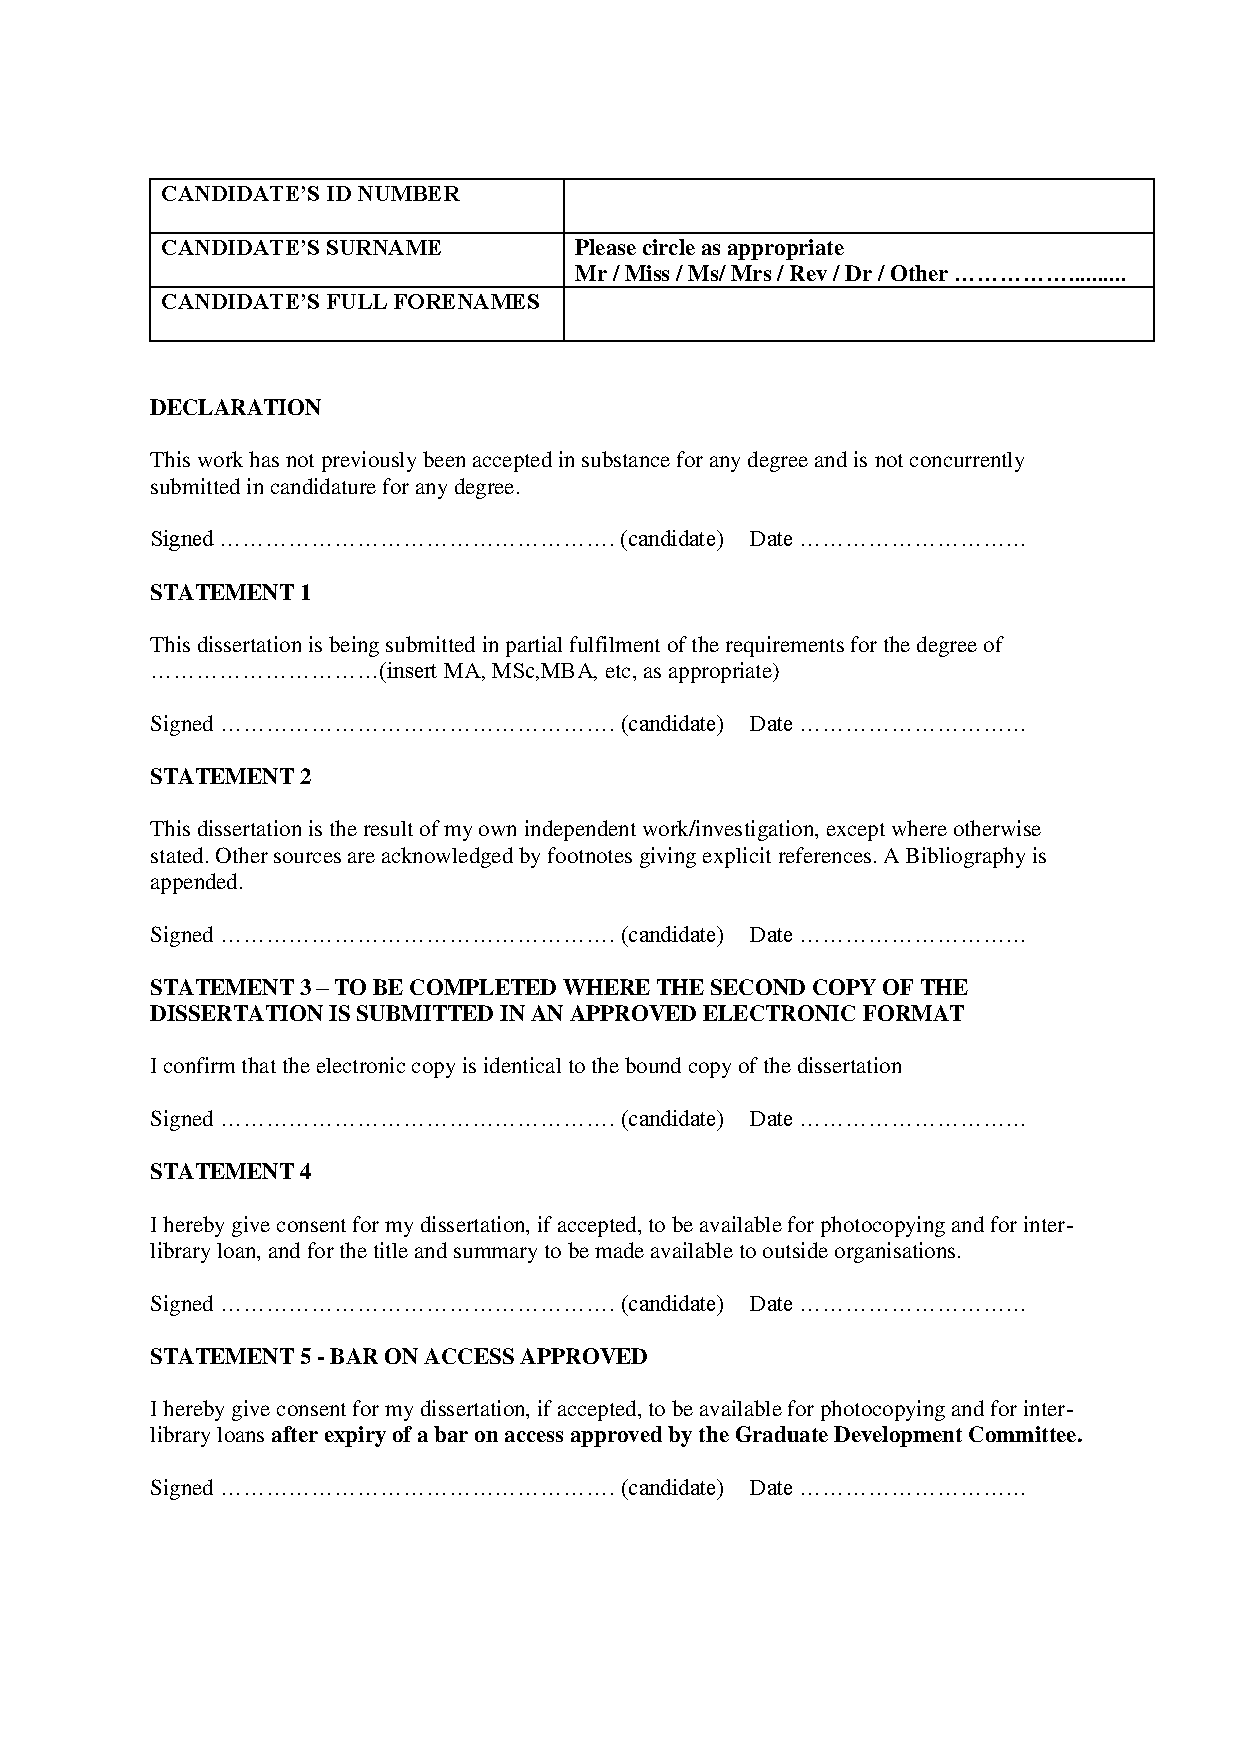
\includepdf[pages={1}]{Dissertation_Declaration_Page.pdf}

\frontmatter
\pagestyle{chapterstyle} %set header-footer style for front matter
\chapter{Executive Summary}

\lipsum[1-9]
\chapter{Acknowledgements}
There have been various people that work in Cardiff University that I would
like to thank for their support during this intense year.


I would like to thank all the lectures of Cardiff University that taught at
the MSc taught program, for enlighten me and my colleges through their teachings.
Also for their continuous support and guidance through the year.
I would like to extend a special thank you to Mrs Joanna Emery for making this
entire year possible for me. Finally, I would like to express my sincere gratitude
to my academic supervisor Dr Vince Knight, for his support, advice and constant
ideas. To whom I lied once during this dissertation; yes the tables were being
overwritten.


\tableofcontents
\listoffigures
\listoftables
\chapter{Summary}

Ever since 1980, when a simple Iterated Prisoner's Dilemma(IPD) computer
tournament was conducted with 13 participants, IPD tournaments and strategies
have been constantly under development. This has inspired scientists to develop
an open source Python library, for reproducing all the research done on the topic
of the IPD. The library is called Axelrod-Python library and alongside various
capabilities, it continuously performs an IPD tournament with the, currently 132,
implemented strategies.

Axelrod-Python library, soon became a powerful tool for the Game Theory society.
Even so, the library was lacking the ability of creating tournaments of a different
topology of that of a round robin one. During this dissertation, the ability to
produce tournaments of a network topology; spatial tournament, was materialized.
Instantly, new questions were raised;such as what are the effects of the topology?

For addressing this questions the following approach was chosen. Identify the
effects of the topology on the performance of the strategies of the library and
does any of this strategies perform well in different tournaments of different
topologies. Thus throughly the research experiments have been conducted. In these
experiments simple and complex networks respectively have been used as topologies
to generate numerous of spatial tournaments. Furthermore, non of the
Axelrod-Python library strategies was characterized as an overall satisfactory
strategy through the experiments. For this reason an new strategy has been trained
using an evolutionary approach.


\mainmatter
\pagestyle{normal} %set header-footer style rest of report


\chapter{Some features of \LaTeX}

\section{Referencing}
We can make make in text citations automatically.
In the `author-year' style we can do this as:
\begin{itemize}
    \item A noun e.g. \textcite{Gillard2014}
    \item In parentheses e.g. \parencite{Gillard2014}
\end{itemize}

\section{Tables}
We can make nicer looking tables in \LaTeX~ using the `booktabs' package.
An example of this can be seen in Table.~\ref{fig:exampletable}.
\begin{table}[h]
\centering
\caption{An example table using the `booktabs' package}
\label{fig:exampletable}
\begin{tabular}{cccccccccc}
\toprule
& \multicolumn{3}{c}{\textbf{ABC}} & \multicolumn{3}{c}{\textbf{ABC}} & \multicolumn{3}{c}{\textbf{ABC}} \\
\cmidrule(lr){2-4}\cmidrule(lr){5-7}\cmidrule(lr){8-10}
\textbf{Example}      & \textbf{A}       & \textbf{B}       & \textbf{C}      & \textbf{A}           & \textbf{B}           & \textbf{C}          & \textbf{A}           & \textbf{B}           & \textbf{C}          \\
\cmidrule(lr){1-1}\cmidrule(lr){2-4}\cmidrule(lr){5-7}\cmidrule(lr){8-10}
0         & 1234      & 1234     & 1234     & 1234          & 1234         & 1234         & 1234        & 1234         & 1234         \\
1         & 1234      & 1234     & 1234     & 1234          & 1234         & 1234         & 1234          & 1234         & 1234         \\
2         & 1234      & 1234     & 1234     & 1234          & 1234         & 1234         & 1234        & 1234         & 1234        \\
3         & 1234      & 1234     & 1234     & 1234          & 1234         & 1234         & 1234        & 1234         & 1234         \\ \bottomrule
\end{tabular}
\end{table}

\section{Footnotes}
We can make footnotes\footnote{This is a footnote} easily.

\section{Sub-figures}
Using the subcaption package we can make side by side figures.
For example see Fig.~\ref{fig:subfigureexample}.

\begin{figure}[h]
\centering
    \begin{subfigure}[t]{0.45\textwidth}
    \centering
        
\includegraphics[width=\linewidth]{image1.png}
    \caption{First sub-figure}
    \end{subfigure}
\hfill
    \begin{subfigure}[t]{0.45\textwidth}\centering
    \centering
        
\includegraphics[width=\linewidth]{image1.png}
    \caption{Second sub-figure}
    \end{subfigure}
~
\caption{Example of using subfigures}
\label{fig:subfigureexample}
\end{figure}


\chapter{Literature Review}
\label{chap:Two}

Following the initial work done by Axelrod, there are many other papers that
have tried to tackle the PD and make their conclusions on cooperation in both a
theoretical and real life setting. In this chapter a review of some of this work
done in the IPD competitions, in spatial and evolutionary game theory will be
carried out.

\section{Tournaments}

In order to identify the condition under which cooperation could emerge
in the game of the Prisoner's Dilemma better, Robert Axelrod held a tournament
in 1980. He invited a number of well-known game theorists to submit strategies
for a computer tournament.  Each strategy has to specify whether to cooperate or
defect based on the history of previous moves made by both players.
Strategies played again
each other as well as a further Random strategy, that would randomly choose
between C and D and with its own twin (same strategy). The tournament was a
round robin with the payoff matrix~\ref{fig:pd_payoff}. All entries knew the
exact length (200 moves) of each game. To improve the reliability of the scores
the entire round robin tournament was repeated five times. Fourteen strategies were
submitted and by the end Tit for Tat was announced the winner. Surprisingly in
the second tournament held where 64 strategies competed and all submitters had
full knowledge of what have happened in the first tournament, Tit for Tat
managed to get first place again\cite{Axelrod1980a}.

As explained in \cite{Axelrod1980b}, Tit for Tat, a simple strategy was
able to beat sophisticated and more complex strategies thanks to three
specific characteristics of the strategy:

\begin{itemize}
  \item Niceness:  A strategy is categorized as nice if it was not the
                    first to defect, or at least, it will not do this until
                    the last few moves.
  \item Forgiveness: The propensity to cooperate in the moves after the
                     opponent defected.
  \item Clarity: After opponents identified that they were playing Tit for Tat
                 choose to cooperate for the rest of the game.
\end{itemize}

The first tournaments were an innovation in combining computer modeling and Game
Theory and in providing insights in the behavior emerging from simple dynamics.
Moreover, Axelrod was the first to speak about niceness, forgiveness and gave an
illustration that cooperation can be a victorious and advantageous strategy.

Another concept that had been developed was the Evolutionary Game Theory (EGT).
EGT is an application of game theory to biological contexts, arising from the
realization that frequency dependent fitness introduces a strategic aspect to
evolution. In 1973, Maynard and Price introduced the concept of Evolutionary
Stable Strategy (ESS), which is an extension of a Nash Equilibrium. If a
population of the same strategies cannot be invaded by any alternative strategy
that is initially rare then that strategy is an ESS. In his third tournament
Axelrod \cite{Axelrod1981} using the same set of strategies (63),
the tournaments introduced a dynamical rule that mimics Darwinian selection.
In this evolutionary computer tournament after a round robin game the score for
each player was evaluated, and the strategies with high score would be adapted
while the lowest ones ones would diminish. In most of these simulations, the
success of Tit-for-Tat was confirmed because the population would end up with
some mutually cooperating strategies prevailed by Tit-for-Tat.

There have been other tournaments, based off of Axelrod’s, exploring different
environments and submitting new strategies. Boyd \& Lorderbaum \cite{Lorberbaum1994}
state that no pure
strategy is evolutionary stable because each can be invaded by the joint effect
of two invading strategies when long term interaction occurs in th repeated game
and future moves are discounted. In 1991 Bendor, Kramer and Stout \cite{The2016}
introduced noise to the IPD. Where noisy randomly flip the choice made by a
strategy. The results of their tournament was that the strategies that were more
generous, cooperated more than their opponents did, were more effective than Tit
for Tat. Moreover, Kerts 2011 conducted a tournament where the payoff matrix was
altered though satisfying the conditions \ref{firstassum}, \ref{secondassum}.

Furthermore, two more notable tournaments took place in 2005 and 2012.
In the 2005 IPD competition a team from the University of Southampton participated
using a group of strategies which won the top three propositions. These strategies
were designed in such why that thought a predetermined sequence of five to ten
moves would recognize each other. Once the two Southampton players recognized
each other they would take up the roles of a ruler and a slave. The ruler
would always cooperate where the slave would defect in order to maximize the
payoff of the ruler. If the opponent was recognized to not being one of the team
then the Southampton player would always choose to defect to minimize the score
of the opponent \cite{Li2011}. Lastly, the Stewart- Plotkin \cite{Stewart2012}
tournament which
consisted of nineteen strategies, including a new set of strategies; the Zero-
determinant(ZD) strategies. The ZD are strategies for the stochastic iterated
prisoner's dilemma, discovered by Press and Dyson in 2012 \cite{Press2012a}.
The ZD apply a linear relationship between their own payoff and that of the opponent.
Some review tournaments are listed on the Table~\ref{tab:tournaments}:

\begin{table}[!hbtp]
    \begin{center}
        \begin{tabular}{ccccc}
            \toprule
            Year     & Reference                  & Number of Strategies & Type     \\
            \midrule
            1979     & \cite{Axelrod1980a}        & 13                   & Standard  \\
            1979     & \cite{Axelrod1980b}        & 64                   & Standard  \\
            1984     & \cite{Axelrod1981}         & 64                   & Evolutionary\\
            1991     & \cite{The2016}          & 13                   & Noisy     \\
            2005     & \cite{Chong2004} & 223                  & Varied    \\
            2012     & \cite{Stewart2012}         & 13                   & Standard   \\
            \bottomrule
        \end{tabular}
    \end{center}
    \caption{An overview of a selection of published tournaments.}\label{tab:tournaments}
\end{table}

In this section the work done for tournaments in the IPD has been cited and analyzed.
Starting with the the work of Axelrod, the reasons the tournaments where organized
and what where the fundings. Moreover, some research that has been generated the following
years are stated. Below, a specialized case of these research will be studied. That
case is that of the spatial structure tournaments.

\section{Spatial Structure Tournaments}

Further research was spawn in 1992 as to how the Prisoner's Dilemma could shade
some insight into physics and biology. Where Nowak and May believed exist potential
dynamics of spatially extended systems. Their tournament was a simple and purely
deterministic spatial version of the PD in a two dimensional lattice. With
players having no memory of the previous rounds and no strategical elaboration.
Thus, the players could either always cooperate or defect. In each round each
player interact with the immediate neighbor. \footnote{In Nowak's and May's
experiment, the result's hold for all three cases that  the player interacts with
4, 6 and 8 neighbors.} They used an evolution rule that after each round
round the nodes with the lowest score in their neighborhood would copy the
strategy of the player with the highest score. This was done to study which
behavior, defection or cooperation , would last. The conclusion was that co-operational
behavior is possible in the PD by using a spatial topology. Nowak produced more
work on the topic on papers of his such as \cite{Nowak1993} (Nowak 1994).
In his subsequent papers Nowak et al. (1994a,b)  different spatial structures
where studied. Including triangular and cubic lattices and a random grid.
It turned out that cooperation can be maintained in spatial models even
for some randomness.

On the other hand,  in \cite{Lindgren1994} players were allowed to have
memory and therefore added complex strategies to the tournament such as Tit for
Tat and  Anti Tit for Tat. This was followed  by the work of
\cite{Brauchli1999} which introduced even more complex strategies. Brauchli et
all compares the spatial model with a randomly mixed model.
A more complex strategy that they have tested was PAVLOV. A win-stay,
lose-switch strategy.  According to their
fundings, there is more cooperative behavior in a spatial structure tournament
and evolution is more less chaotic than in unstructured populations. Also as
stated, generous variants of PAVLOV are found to be very successful
strategies in playing the Iterated Prisoner's Dilemma.

Spatial topology has been defined by most scholars as a square lattice where
the nodes - players only interact with their neighborhoods. Including connections
between four or eight nearest neighbor sites, Neuman's or Moore's, according to
Figure~\ref{fig:neighborhood}. A square lattice is a graph and one could argue
that a round robin tournament itself is the complete graph on all players
\cite{Bela}. But in the above papers
no authors defined the topology as a graph, apart from \cite{Meng2015}.

In \cite{Meng2015}, an interesting approach was used. They presented a new
spatial prisoner's dilemma game model in which the neighborhood size was
increased onto two interdependent lattices. They implement the utility by
integrating the payoff correlations between two lattices. A player would mimic a
random player in his next move, base on a function that consider the utility of
the player. It was characterized as a most realistic scenario.

Real life interactions are more likely to be like any given graph depending on
the industry than a complete graph. Fatha et all \cite{Szabo2007}, have
considered a numerous of graphs, such as :

\begin{itemize}
  \item Lattice, the interaction network is defined by the sites of a lattice.
   the distance between a pair does not exceed a given value.
   The most frequently used structure is the square lattice with von Neumann
   neighborhood and Moore neighborhood.
  \item Small word, a graph that is created from a square lattice by randomly
   rewiring a fraction of connections in a way that conserve the degree for
   each site.
  \item Scale-free graphs, a network that has a power-law degree distribution, regardless of
   any other structure.
  \item Evolving networks, networks that change as a function of time (this will
      not be considered in this dissertation).
\end{itemize}

The major theme of their review was how the graph structure of interactions could
modify long term behavioral patterns emerging in evolutionary games.
These graphs compose only a small fraction of graphs that exist. In this
dissertation we will consider a list of graphs.
 %add list when i actually know

\section{Axelrod Python Library}

The Axelrod library \cite{axelrodproject} is an open source Python package that allows for
reproducible game theoretic research into the Iterated Prisoner's Dilemma
\url{https://github.com/Axelrod-Python}.
For many of the tournaments aforementioned the original source code is almost never
available and in no cases is the available code well-documented, easily modified
or released with significant test suites. Due to that reproducing the results
has not been an easy task.

However, Axelrod library manages to provide such a resource, with facilities for
the design of new strategies and interactions between them, as well as
conducting tournaments and ecological simulations for populations of strategies.

Strategies are implemented as classes which have a single method, \texttt{strategy()}.
It only takes one argument, which is the opponent's previous moves and returns
an action. These actions can be either to cooperate C or to defect D. At thins
moment the Axelrod library consists of 131 strategies.Can be found in the Appendix.
As an example we can see in Listing~\ref{lst:tit_for_tat} the source code for the
famous strategy Tit for Tat.

\begin{listing}[H]
\usemintedstyle{tango}
\begin{minted}
[
frame=lines,
framesep=2mm,
baselinestretch=1.2,
bgcolor=LightBlue,
fontsize=\footnotesize,
linenos
]
{python}

class TitForTat(Player):
    """
    A player starts by cooperating and then mimics
    the previous action of the opponent.

    Note that the code for this strategy is written
    in a fairly verbose way. This is done so that it
    can serve as an example strategy for those who
    might be new to Python.
    """

    # These are various properties for the strategy
    name = 'Tit For Tat'
    classifier = {
        'memory_depth': 1,  # Four-Vector = (1.,0.,1.,0.)
        'stochastic': False,
        'makes_use_of': set(),
        'inspects_source': False,
        'manipulates_source': False,
        'manipulates_state': False
    }

    def strategy(self, opponent):
        """This is the actual strategy"""
        # First move
        if len(self.history) == 0:
            return C
        # React to the opponent's last move
        if opponent.history[-1] == D:
            return D
        return C
\end{minted}
\caption{Tit for Tat source code.}
\label{lst:tit_for_tat}
\end{listing}

Additionally, the tournament class is responsible for coordinating the play of
generated matches. It achieves that by calling a match generator class which
returns all the single match parameters, such as turns, the game and the noise.
Axelrod has the capability to write out the results into a csv file and also out
put plots with the ranks of the strategies.

Furthermore, a basic tournament of 200 turns, 100 repetitions and the 131
strategies that exist in the library is being produced continuously. The current
winner is called PSO gambler and it is a look up strategy. It uses a lookup
table with probability numbers generated using a Particle Swarm Optimisation
(PSO) algorithm, the sourse code can be found here :
 \url{http://axelrod.readthedocs.io/en/latest/_modules/axelrod/strategies/gambler.html?highlight=Gambler})
 and a description of how this strategy was trained is given here:
 \url{https://gist.github.com/GDKO/60c3d0fd423598f3c4e4}.
It uses a 64-key lookup table (keys are 3-tuples consisting of the opponent's
starting actions, the opponent's recent actions, and our recent action) to
decide whether to cooperate (C) or defect (D). The actions for each key were
generated using an evolutionary algorithm.

To reproduce a basic tournament with the 131 strategies using Axelrod :

\begin{listing}[ht]
\begin{minted}
[
frame=lines,
framesep=2mm,
baselinestretch=1.2,
bgcolor=LightGray,
fontsize=\footnotesize,
linenos
]
{python}

>>> import axelrod
>>> strategies = [s() for s in axelrod.ordinary_strategies]
>>> tournament = axelrod.Tournament(strategies)
>>> results = tournament.play()
>>> plot = axelrod.Plot(results)
>>> p = plot.payoff()
>>> p.show()
\end{minted}
\caption{A simple set of commands to create a basic tournament. The
    output is shown in Figure~\ref{fig:axelrodplots}.}
\end{listing}

 Here are illustrated the results of the last tournament :
 \newpage

\begin{figure}[h]
\centering
    \begin{subfigure}[t]{0.7\textwidth}
    \centering
        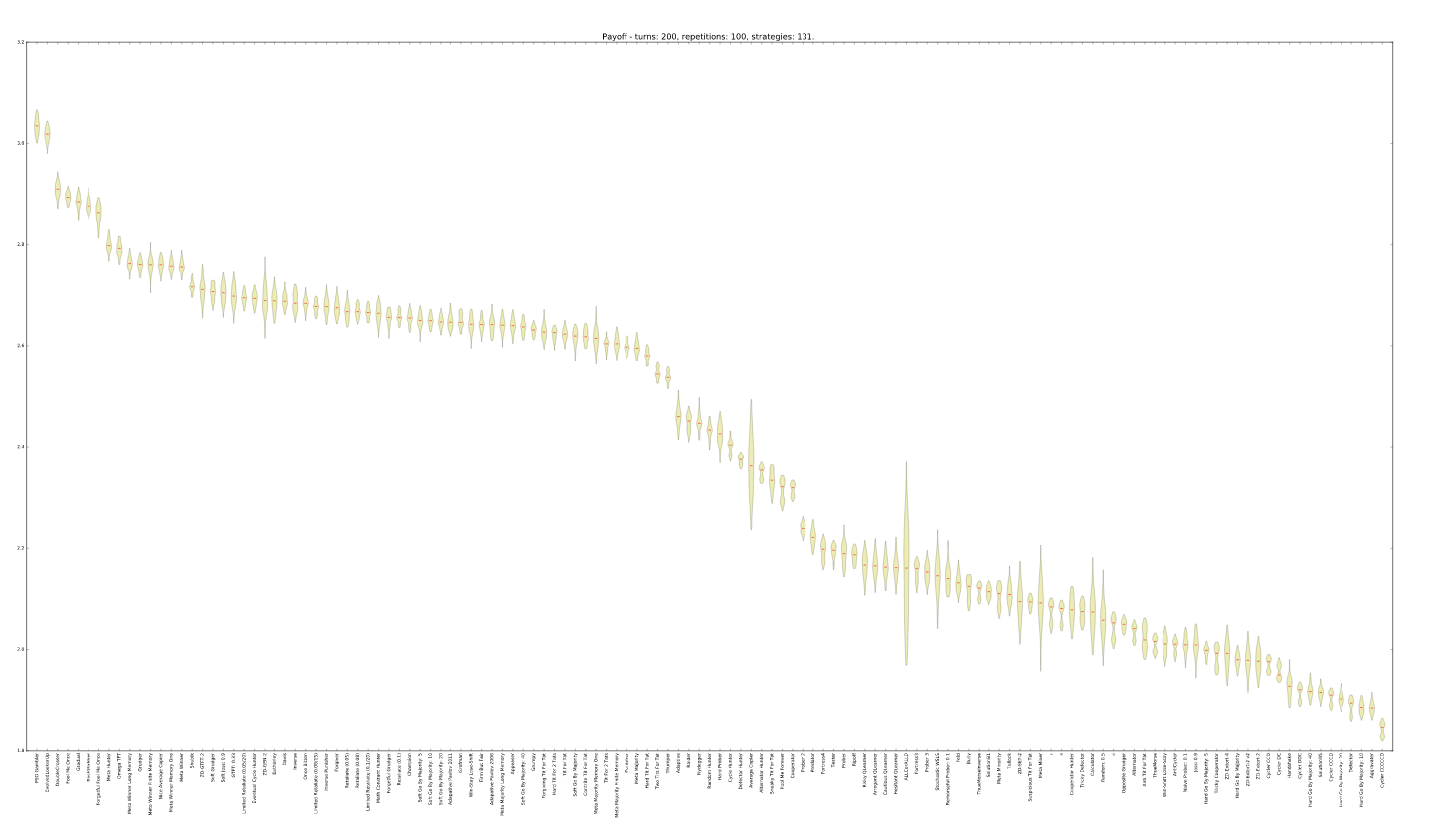
\includegraphics[width=\linewidth]{chapter-two/axl.png}
    \caption{Ranked violin plot}
    \end{subfigure}
\hfill
    \begin{subfigure}[t]{0.70\textwidth}\centering
    \centering
        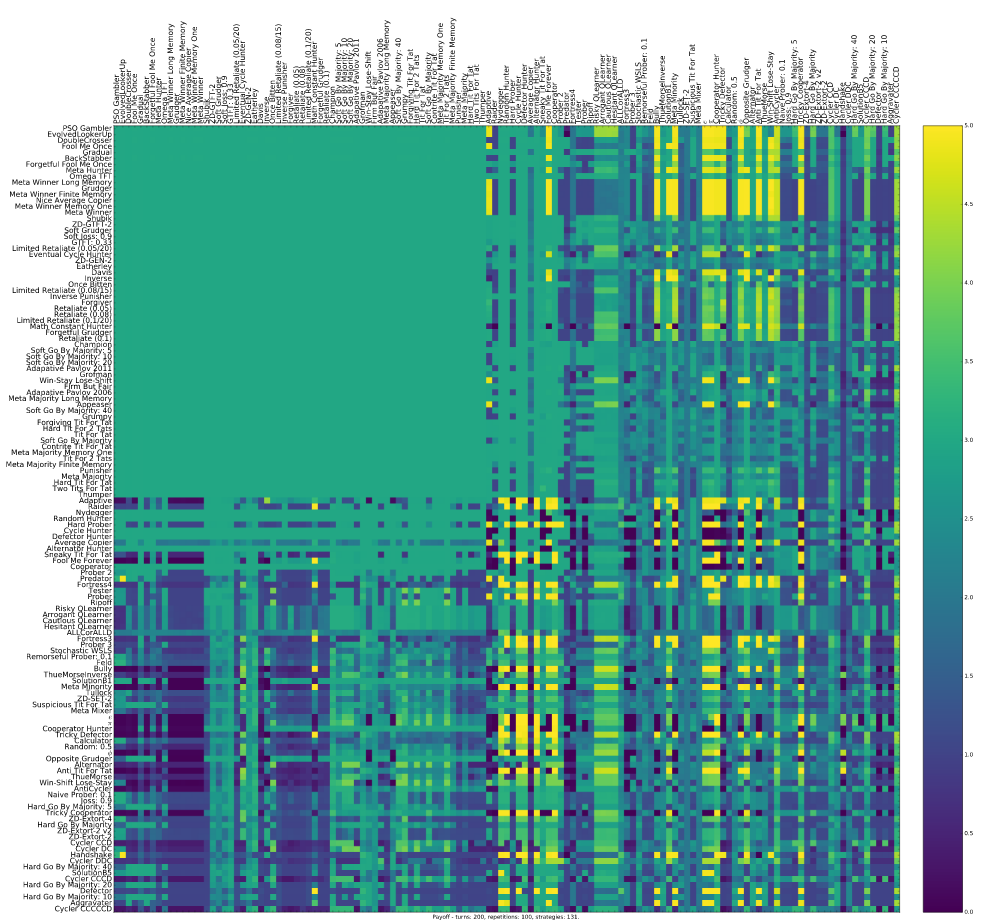
\includegraphics[width=\linewidth]{chapter-two/axl1.png}
    \caption{Payoffs}
    \end{subfigure}
~
\caption{Result Plots. (a) Ranked violin plot, the mean utility of each player.
(b) Payoffs, the pair wise utilities of each player.}
\label{fig:axelrodplots}
\end{figure}

More details for the documentation of the library can be found here :
\url{https://axelrod.readthedocs.io/en/latest/index.html}.
Because is an open source library it makes it easy to contribute to it and
make modifications needed for this dissertation.

\chapter{Implementation of spatial tournaments}
\label{chap:Three}

\section{Introduction}
In this chapter some initial experiments and their results are discussed.
These experiments have been performed using three chosen topologies and two
different sizes of tournaments. Emphasis is given in the analysis of the
results and identification of strategies behaviors. In addition, the source code
committed to the Axelrod-Python library to implement a spatial topology are
discussed, as well as two important aspects of developing
test driven development and version control.

\subsection{Code Discussion}

As analyzed in \autoref{chap:Two}, the Axelrod library uses a
\texttt{Tournament} class to run any given tournament. The \texttt{Tournament}
class itself calls upon another class, the \texttt{Match Generator}, which is
responsible for generating matches.
In the case of a standard round robin, there is a \texttt{RoundRobinTournament} class
and a \texttt{RoundRobinMatches} class that generates matche parameters for each 2 player
tuple. The parameters and the indices of the pair are used
by the \texttt{build\_single\_match} method. A generator that lives within the
match generator class.
For a round robin tournament the structure of the code is illustrated
in~\ref{fig:round_robin_structure}.


\begin{figure}
\centering
    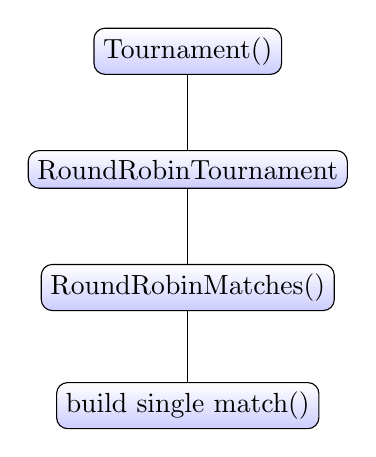
\begin{tikzpicture}[sibling distance=10em,
      every node/.style = {shape=rectangle, rounded corners,
        draw, align=center,
        top color=white, bottom color=blue!20}]]
      \node {Tournament()}
        child { node {RoundRobinTournament}
          child { node {RoundRobinMatches()}
            child { node {build single match()} } }
           };
    \end{tikzpicture}
  \caption{Code structure for a Round Robin tournament.}
  \label{fig:round_robin_structure}
\end{figure}

In order to implement a Spatial topology tournament a similar approach is
needed. Firstly a new \texttt{Match Generator} class was written.  The
\texttt{SpatialMatches} is a class that generates spatially-structured matches.
In these matches, players interact only with their neighbors rather than the
entire population. According to \cite{Archdeacon1996} graphs can be represented
in many different ways, one of which is by lists of edges.  Due to a various
number of python packages that are used for graph manipulation,
a more generalized representation of the edges has be selected. Thus edges
are passed as an argument and \texttt{SpatialMatches} only creates matches
between the
ending nodes of these edges. Finally the class \texttt{SpatialTournament} runs
the spatial tournament. A representation of the code structure now, that the
spatial tournaments have been added, can be seen in
Figure~\ref{fig:spatial_structure}

\begin{figure}
\centering
    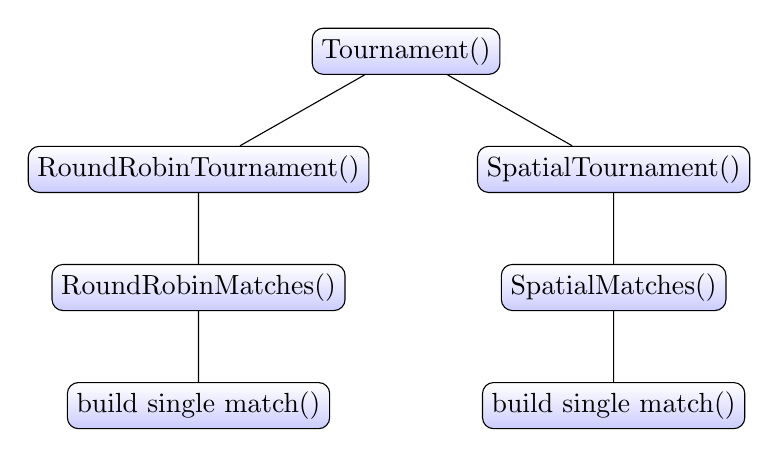
\begin{tikzpicture}[sibling distance=15em,
      every node/.style = {shape=rectangle, rounded corners,
        draw, align=center,
        top color=white, bottom color=blue!20}]]
      \node {Tournament()}
        child { node {RoundRobinTournament()}
          child { node {RoundRobinMatches()}
            child { node {build single match()} } }}
        child { node {SpatialTournament()}
          child { node {SpatialMatches()}
            child { node {build single match()} } }
           };
    \end{tikzpicture}
  \caption{Code structure for when Round Robin and Spatial tournaments are
           implemented.}
  \label{fig:spatial_structure}
\end{figure}

The Axelrod-Python library is developed using a Test Driven Development (TDD) approach.
All the components are automatically tested using a combination of unit,
property and integration tests (using \url{travis-ci.org}).
Once a new feature is added to the library, a corresponding test must also be
written. The tests are used to ensure compatibility and ensure that the expected
results are returned.
In~\cite{Developer} Percival explains from his personal
experiences the importance of TDD and having tests for every single line of code.
For the spatial tournament a
new unit test have been added. Unit tests are used to invoke a unit of work and
check that the behavior is expected. A unit of work can be any single logical
functional use in the system. In summary, unit tests help to write clean and bug
free code~\cite{Developer}. The unit tests for the \texttt{SpatialTournament} can
be found below ~\ref{lst:test_spatial_tournament}.

\begin{listing}[H]
\usemintedstyle{tango}
\begin{minted}
[
frame=lines,
framesep=2mm,
baselinestretch=1.2,
bgcolor=LightBlue,
fontsize=\footnotesize,
linenos
]
{python}
class TestSpatialTournament(unittest.TestCase):

    @classmethod
    def setUpClass(cls):
        cls.game = axelrod.Game()
        cls.players = [s() for s in test_strategies]
        cls.test_name = 'test'
        cls.test_repetitions = test_repetitions
        cls.test_turns = test_turns
        cls.test_edges = test_edges

    def test_init(self):
        tournament = axelrod.SpatialTournament(
            name=self.test_name,
            players=self.players,
            game=self.game,
            turns=self.test_turns,
            edges=self.test_edges,
            noise=0.2)
        self.assertEqual(tournament.match_generator.edges, tournament.edges)
        self.assertEqual(len(tournament.players), len(test_strategies))
        self.assertEqual(tournament.game.score(('C', 'C')), (3, 3))
        self.assertEqual(tournament.turns, 100)
        self.assertEqual(tournament.repetitions, 10)
        self.assertEqual(tournament.name, 'test')
        self.assertTrue(tournament._with_morality)
        self.assertIsInstance(tournament._logger, logging.Logger)
        self.assertEqual(tournament.noise, 0.2)
        anonymous_tournament = axelrod.Tournament(players=self.players)
        self.assertEqual(anonymous_tournament.name, 'axelrod')
\end{minted}
\caption{Source code for TestSpatialTournament class, which is for testing the
         spatial tournaments.}
\label{lst:test_spatial_complete_tournament}
\end{listing}

\texttt{TestSpatialTournament()} it a simple class for a unittest written for
the spatial tournaments. In~\ref{lst:test_spatial_tournament}, whether
the values of the attributes were passed correctly is being tested. Also whether
the scores are as anticipated. In~\ref{lst:test_spatial_complete_tournament},
another test is shown. Here the results of a spatial tournament on a complete graph
are compared to those of a round robin one.

\begin{listing}[H]
\usemintedstyle{tango}
\begin{minted}
[
frame=lines,
framesep=2mm,
baselinestretch=1.2,
bgcolor=LightBlue,
fontsize=\footnotesize,
linenos
]
{python}
@given(strategies=strategy_lists(strategies=deterministic_strategies,
                                     min_size=2, max_size=2),
           turns=integers(min_value=1, max_value=20))
    def test_complete_tournament(self, strategies, turns):
        """
        A test to check that a spatial tournament on the complete multigraph
        gives the same results as the round robin.
        """
        players = [s() for s in strategies]
        # edges
        edges=[]
        for i in range(0, len(players)) :
            for j in range(i, len(players)) :
                edges.append((i, j))
        # create a round robin tournament
        tournament = axelrod.Tournament(players, turns=turns)
        results = tournament.play()
        # create a complete spatial tournament
        spatial_tournament = axelrod.SpatialTournament(players, turns=turns,
                                                       edges=edges)
        spatial_results =  spatial_tournament.play()
        self.assertEqual(results.ranked_names, spatial_results.ranked_names)
        self.assertEqual(results.nplayers, spatial_results.nplayers)
        self.assertEqual(results.nrepetitions, spatial_results.nrepetitions)
        self.assertEqual(results.payoff_diffs_means,
                                         spatial_results.payoff_diffs_means)
        self.assertEqual(results.payoff_matrix,
                                              spatial_results.payoff_matrix)
        self.assertEqual(results.payoff_stddevs,
                                             spatial_results.payoff_stddevs)
        self.assertEqual(results.payoffs, spatial_results.payoffs)
        self.assertEqual(results.cooperating_rating,
                                         spatial_results.cooperating_rating)
        self.assertEqual(results.cooperation, spatial_results.cooperation)
        self.assertEqual(results.normalised_cooperation,
                                     spatial_results.normalised_cooperation)
        self.assertEqual(results.normalised_scores,
                                          spatial_results.normalised_scores)
        self.assertEqual(results.good_partner_matrix,
                                        spatial_results.good_partner_matrix)
        self.assertEqual(results.good_partner_rating,
                                        spatial_results.good_partner_rating)
\end{minted}
\caption{Source code for testing a complete spatial tournament.}
\label{lst:test_spatial_tournament}
\end{listing}

The source code for the spatial tournaments and the tests can be found
in the Axelrod-Python library. The library is available at
\url{https://github.com/Axelrod-Python},
which is a hosted git repository. This introduces another important aspect
of software development: version control systems (VCS). As stated in \cite{Developer}
TDD and VCS go hand in hand. VCS, is a tool that manages and tracks different
versions of software~\cite{Vogel2014}. Lines of codes are deleted, implementing
errors occur and programmers forget. Thus, having the ability to go back to any
given point can be very important. Git is a specific powerful and famous VCS. It
was invented by Linus Torvalds and span to life in April 2005~\cite{Vogel2014}.

The Axelrod-Python library is a project which includes numerous contributors.
Any given addition to the
library has to be submitted by a pull request. Each submission is then
reviewed by members of the core team. This applies to the spatial tournament as well.
In Figure~\ref{fig:github} a conversation containing comments and corrections
can be seen.

\begin{figure}[H]
\centering
    \begin{subfigure}[H]{0.7\textwidth}
    \centering
        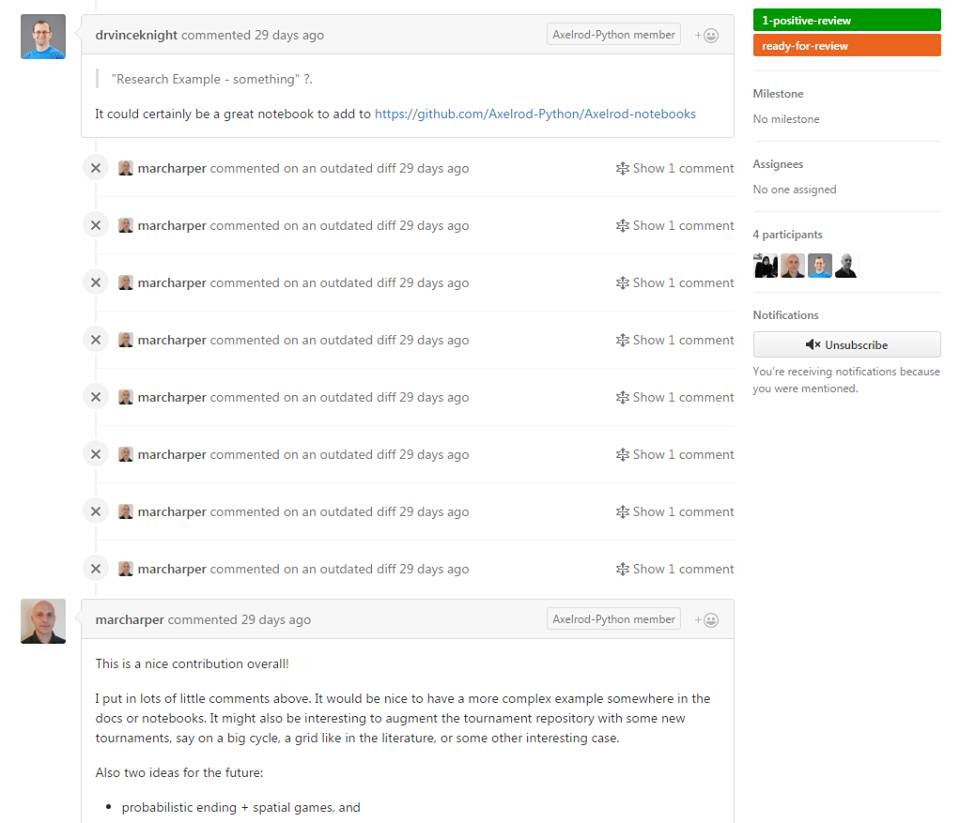
\includegraphics[width=\linewidth]{chapter-three/comments.jpeg}
    \caption{Comments and corrections.}
    \end{subfigure}
\hfill
    \begin{subfigure}[H]{0.7\textwidth}\centering
    \centering
        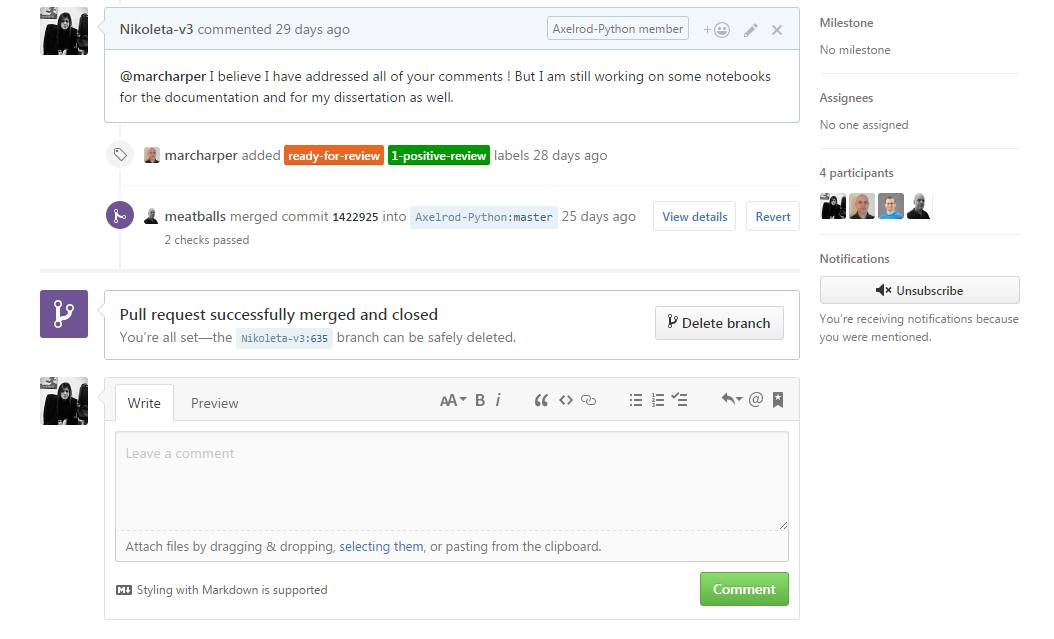
\includegraphics[width=\linewidth]{chapter-three/merging.jpeg}
    \caption{Merging a pull request after reviews.}
    \end{subfigure}
\caption{On line communication and reviews, through GitHub,
         with members of the Axelrod-Python library.}
\label{fig:github}
\end{figure}

O. Campbell and M. Harper are 2 of the 4 core contributors of the library.
Their work, in company to other contributors included myself, had an impact on
the Game Theory society. The project involves various research topics of
the IPD, such as Noise tournaments, Probabilistic ending, Spatial tournaments,
strategies from different works and authors and the capability
of reproducing any of these given tournaments. This led to a publication to be
achieved earlier in 2016~\cite{Knight2016}.

In the next section an overview and a summary of the initial experiments
performed is given.


\subsection{Experiment and the three topologies}

In this chapter three simple spatial topologies are considered, all with
deterministic neighborhood size. These will be used to begin to understand how
topology can affect the outcome of tournaments
and which strategies tend to perform well. The three topologies considered are
well represented in the literature :  %\cite{}:

\begin{itemize}
    \item A cyclic network: the neighbourhood size is 2. % include specific references
    \item A periodic lattice: the neighbourhood size is 4. % include specific references
    \item A complete graph: the neighbourhood size is \(N-1\) (where \(N\) is
        the number of total strategies. This corresponds to a round robin
        tournament. % References
\end{itemize}

Figure~\ref{fig:networks}, shows an example of all the aforementioned topologies.

\begin{figure}[!hbtp]  % http://drvinceknight.blogspot.co.uk/2013/12/explaining-floats-in-latex.html
\centering
    \begin{subfigure}[h]{0.45\textwidth}
    \centering
        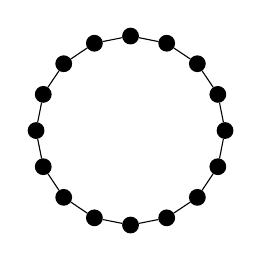
\begin{tikzpicture}[scale=1.2]

   \node (00) [draw, circle, inner sep=2pt,fill] at ( 1.,  0.) {} ;
   \node (01) [draw, circle, inner sep=2pt,fill] at ( 0.92387953,  0.38268343) {} ;
   \node (02) [draw, circle, inner sep=2pt,fill] at ( 0.70710678,  0.70710678) {} ;
   \node (03) [draw, circle, inner sep=2pt,fill] at ( 0.38268343,  0.92387953) {} ;
   \node (04) [draw, circle, inner sep=2pt,fill] at ( 6.12323400e-17,   1.00000000e+00) {} ;
   \node (05) [draw, circle, inner sep=2pt,fill] at (-0.38268343,  0.92387953) {} ;
   \node (06) [draw, circle, inner sep=2pt,fill] at (-0.70710678,  0.70710678) {} ;
   \node (07) [draw, circle, inner sep=2pt,fill] at (-0.92387953,  0.38268343) {} ;
   \node (08) [draw, circle, inner sep=2pt,fill] at (-1.00000000e+00,   1.22464680e-16) {} ;
   \node (09) [draw, circle, inner sep=2pt,fill] at (-0.92387953, -0.38268343) {} ;
   \node (10) [draw, circle, inner sep=2pt,fill] at (-0.70710678, -0.70710678) {};
   \node (11) [draw, circle, inner sep=2pt,fill] at (-0.38268343, -0.92387953) {};
   \node (12) [draw, circle, inner sep=2pt,fill] at (-1.83697020e-16,  -1.00000000e+00) {};
   \node (13) [draw, circle, inner sep=2pt,fill] at ( 0.38268343, -0.92387953) {};
   \node (14) [draw, circle, inner sep=2pt,fill] at ( 0.70710678, -0.70710678) {};
   \node (15) [draw, circle, inner sep=2pt,fill] at ( 0.92387953, -0.38268343) {};

  \draw (15)--(00)--(01)--(02)--(03)--(04)--(05)--(06)--(07)--(08)--(09)--(10)--(11)--(12)--(13)--(14)--(15);
\end{tikzpicture}

    \caption{Cyclic network.}
    \end{subfigure}
\hfill
    \begin{subfigure}[h]{0.52\textwidth}\centering
    \centering
        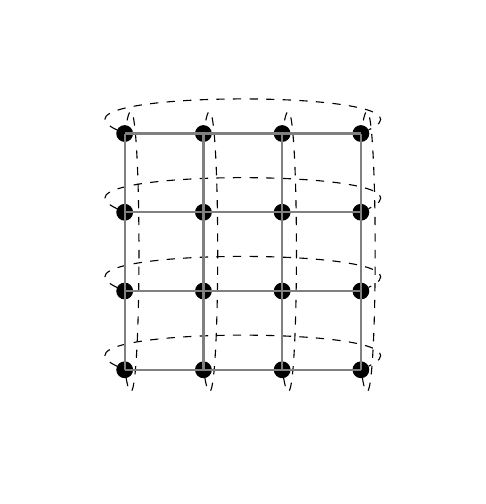
\begin{tikzpicture}

        % First column (tikz has the ability to use loops but I'm drawing it
        % this way so you see how.
        \node (00) [draw, circle, inner sep=2pt,fill] at (0, 0) {};
        \node (01) [draw, circle, inner sep=2pt,fill] at (0, 1) {};
        \node (02) [draw, circle, inner sep=2pt,fill] at (0, 2) {};
        \node (03) [draw, circle, inner sep=2pt,fill] at (0, 3) {};

        % Second column
        \node (10) [draw, circle, inner sep=2pt,fill] at (1, 0) {};
        \node (11) [draw, circle, inner sep=2pt,fill] at (1, 1) {};
        \node (12) [draw, circle, inner sep=2pt,fill] at (1, 2) {};
        \node (13) [draw, circle, inner sep=2pt,fill] at (1, 3) {};

        % Third column
        \node (20) [draw, circle, inner sep=2pt,fill] at (2, 0) {};
        \node (21) [draw, circle, inner sep=2pt,fill] at (2, 1) {};
        \node (22) [draw, circle, inner sep=2pt,fill] at (2, 2) {};
        \node (23) [draw, circle, inner sep=2pt,fill] at (2, 3) {};

        % Fourth column
        \node (30) [draw, circle, inner sep=2pt,fill] at (3, 0) {};
        \node (31) [draw, circle, inner sep=2pt,fill] at (3, 1) {};
        \node (32) [draw, circle, inner sep=2pt,fill] at (3, 2) {};
        \node (33) [draw, circle, inner sep=2pt,fill] at (3, 3) {};


        % I am drawing the periodic boundaries before the rest of the grid
        % so that they appear 'behind' the rest of the images.
        % Draw the period horizontal boundary
        \draw[dashed] (00) to[out=155,in=25 ] (30);
        \draw[dashed] (01) to[out=155,in=25 ] (31);
        \draw[dashed] (02) to[out=155,in=25 ] (32);
        \draw[dashed] (03) to[out=155,in=25 ] (33);

        % Draw the period vertical boundary
        \draw[dashed] (00) to[out=-80,in=80] (03);
        \draw[dashed] (10) to[out=-80,in=80] (13);
        \draw[dashed] (20) to[out=-80,in=80] (23);
        \draw[dashed] (30) to[out=-80,in=80] (33);

        % Draw a grid (this is a tikz shortcut)
        \draw[style=help lines,thick] (0,0) grid  (3,3);
\end{tikzpicture}

    \caption{Periodic lattice with degree 4 network.}
    \end{subfigure}
\hfill
    \begin{subfigure}[h]{0.52\textwidth}\centering
    \centering
    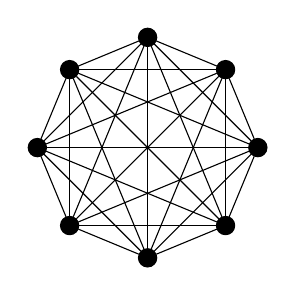
\begin{tikzpicture}
  \graph {subgraph K_n [n=8,clockwise, nodes={draw, circle, fill=black, scale=0.7}, empty nodes,radius=2cm]};
\end{tikzpicture}

    \caption{A complete or round robin network.}
    \end{subfigure}
\caption{Network topologies.}
\label{fig:networks}
\end{figure}


For each topology, a fixed number of strategies out of the 132 of Axelrod-Python
library (1.7.0) are chosen randomly. The number of strategies define the size of the
tournament. In the following experiments, the tournament size can be either
five or fifty. In chapter~\ref{chap:Four} a more expansive tournament size range is
considered for the corresponding analysis. %replace when merge chapter 4

Subsequently, the strategies are allocated on the graph, based
on the topology, and they compete with their neighbors in a IPD tournament.
For the cyclic and lattice topology, once the first game is complete,
the strategies are randomly shuffled and allocated on a graph again. This aims
to ensure that their particular position on the network is taken in to account.
This shuffle is repeated 10 times. The selection of strategies is repeated 100 times
and each tournament of an IPD consists of 200 turns and 10 repetitions.
Algorithm~\ref{simple-experiment-rules} illustrates these rules.

\begin{algorithm}
  \caption{Simple Experiments Rules}\label{simple-experiment-rules}
  \begin{algorithmic}
  \Procedure{Running Experiment}{}
  \BState \emph{loop}:
  \For {$\textit{i} \gets \textit{ 0 to 100}$}
  \State $player \gets \textit{random.strategies}$.
  \For {$i \gets \textit{0 to 10}$}
  \State $G \gets \textit{create.graph}$.
  \State $edges \gets \textit{G.egdes}$
  \State $results \gets \textit{play.tournament}$.
  \emph{loop}.
  \EndFor
  \EndFor
  \EndProcedure
  \end{algorithmic}
\end{algorithm}

% seeds allow us
% reproduce the same players and tournaments.},
% You're going in to to many details here: the reader could potentially have no
% idea what Numpy is. If you write this out with pseudo code you can simply say
% that you're looping over seeds and then include some nice reference/comment
% about why you're doing that.

Due to the high computational cost of the analysis considered, the Cardiff
University's super computer is used. All the scripts and pbs file, for
communicating with Raven, can be found on github :
\url{https://github.com/jobs/Nikoleta-v3}.

For the data preparations and analysis the following libraries have been used:
\begin{multicols}{2}
  \begin{itemize}
    \item Numpy 1.11.1:
    \item Pandas 0.18.1:
    \item Matplotlib 1.5.1:
    \item Statsmodels 0.6.1:
    \item Networkx 1.11:
  \end{itemize}
\end{multicols}

Furthermore, some simple functions for measures such as neighborhood scores
have been written.

% I have to create a repository with all the files for the dissertation and clean
% thing up a little bit. Then I will add the new link here. and a message 'Like my page :D'

% Haha: good idea :) We'll also talk about using something like zenodo.org to
% 'freeze' your data. We should talk about this.

In the next section, preliminary analysis of the experiments aforementioned
is described. Followed by, an intense analysis in section~\ref{sub:analyzing_the_effect_of_the_topologies}.
There, the concept of winning ratio and normalized average score are introduced.
Finally, the results have been summarized in~\ref{sub:summary}, offering further
avenues of research.


\subsection{Initial Analysis}
\label{sub:initial_analysis}
For each of the tournaments run, the following parameters are recorded:

\begin{multicols}{3}
  \begin{itemize}
    \item players list
    \item seed
    \item parameter
    \item player index
    \item player name
    \item cooperating ratio
    \item degree
    \item neighbors
    \item neighborhood size
    \item ranking
    \item scores
    \item normalized scores
    \item average score
    \item R
    \item P
    \item S
    \item T
    \item connectivity
    \item clustering
    \item cliques
    \item neighbors scores
    \item normalized neighbors score
    \item normalized average neighborhood score
  \end{itemize}
\end{multicols}

This section will describe the findings of a basic statistical analysis of these
records.

For the spatial tournaments, for both tournament sizes (5 and 50),
1000 tournaments have been played. Containing 100 different strategy sets, each of
which playing 10 tournaments.

Moreover, for the cyclic experiments as shown in Table~\ref{sum-cicle}, the degree is
and the payoffs are fixed for both tournament sizes. For tournaments of size 5,
the mean average score is 2.45, with a minimum value of 0.0175 and a maximum
value of 4.95. The mean average score of the neighbors score is 980.95 with a
standard deviation of 219.87.
The mean average score does not seem to differ for size equal to 50, which is at
2.39. Though, in the experiment with a size of fifty a strategy
achieved an average score of 0. Additionally the average score of the neighbors ranges
from 19.30 to 1884.5. Concerning the graph measures, as explained in [chapter 2],
clustering coefficient is zero and connectivity fixed to 2.
% Also I forget, but assuming you have described what these things mean in C2,
% you should remind the reader and just point them to C2.

% This table looks good BUT (IMPORTANT) Read these (and then improve all your
% tables)
% - http://www.howtotex.com/packages/improve-your-tables-with-booktabs/
% - https://www.inf.ethz.ch/personal/markusp/teaching/guides/guide-tables.pdf
%   (particularly the before and after slide)
\begin{table}[!hbtp]
\centering
\begin{adjustbox}{width=1\textwidth}
\small
\begin{tabular}{@{}|l|l|l|l|l|l|l|l|l|l|@{}}
\toprule
Cyclic & \multicolumn{3}{c|}{tournament size 5 and 50} & \multicolumn{3}{c|}{tournament size 5} & \multicolumn{3}{c|}{tournament size 50}                             \\\midrule

       & (R,P,S,T) & degree & connectivity & average score & average neighbors score & clustering & average score & average neighbors score & clustering \\\midrule
mean   & (3,1,0,5) & 2.0    & 2.0          & 2.45      & 980.95            & 0.00       & 2.39     & 957.23             & 0.00       \\\midrule
std    & (0,0,0,0) & 0.0    & 0.0          & 0.74      & 219.87             & 0.00       & 0.77    & 231.32              & 0.00       \\\midrule
min    & (3,1,0,5) & 2.0    & 2.0          & 0.01      & 141.55             & 0.00       & 0.00    & 19.30              & 0.00       \\\midrule
max    & (3,1,0,5) & 2.0    & 2.0          & 4.95     & 1756.50             & 0.00       & 5.00    & 1884.50             & 0.00       \\ \bottomrule
\end{tabular}
\end{adjustbox}
\caption{Summary table for topology circle.}
\label{sum-cicle}
\end{table}

For the lattice topologies a table that summarizes the data is shown in Table
~\ref{sum-lattice}. For both size values the payoffs are the same (\(R=3, P=1, S=0, T=5\))
and the degree is fixed at 4. For size 5 the mean average score
varies between 0.018 and 4.97. The average score of the neighbors varies between
832.67 and 2895.42. Much higher than both the cyclic experiments achieved. This
is understood to be based on the fact that the number of neighbors is now doubled.
For size 5 the mean score is 0.57 and the mean average neighbor score 2.45.
The clustering coefficient is 1 and for size 50 is 0.5.
This shows that in the lattice example the strategies tend to create groups.
% What do you mean about 'groups'. I don't disagree, just curious.

\begin{table}[!hbtp]
\centering
\begin{adjustbox}{width=1\textwidth}
\small
\begin{tabular}{@{}|l|l|l|l|l|l|l|l|l|l|@{}}
\toprule
Lattice & \multicolumn{3}{c|}{tournament size 5 and 50} & \multicolumn{3}{c|}{tournament size 5} & \multicolumn{3}{c|}{tournament size 50}                            \\ \midrule
       & (R,P,S,T) & degree & connectivity & average score & average neighbors score & clustering & average score & average neighbors score & clustering \\ \midrule
mean   & (3,1,0,5) & 4.0    & 4.0          & 2.45      & 1958.56           & 1.0        & 2.39      & 1912.74             & 0.5        \\ \midrule
std    & (0,0,0,0) & 0.0    & 0.0          & 0.57      & 287.63            & 0.0        & 0.59      & 268.37              & 0.00       \\ \midrule
min    & (3,1,0,5) & 4.0    & 4.0          & 0.52      & 1059.77           & 1.0        & 0.01      & 832.67              & 0.5        \\ \midrule
max    & (3,1,0,5) & 4.0    & 4.0          & 4.24     & 2518.70            & 1.0        & 4.97      & 2895.42             & 0.5        \\ \bottomrule
\end{tabular}
\end{adjustbox}
\caption{Summary table for the lattice topology.}
\label{sum-lattice}
\end{table}


Finally, for the round robin tournaments, 100 tournaments were performed for both
sizes. Parameters such as neighborhood size and neighbor's score
were not computed for the round robin topology. This is because all players
interact with each other thus there were not any additional information to be
gained. In Table~\ref{sum-rr}, the average score the strategies achieved
in this topology for both sizes is shown. In a tournament of size 50, the mean average
score is 2.39 with a standard deviation of 0.335.

\begin{table}[H]
\centering
\begin{tabular}{|l|l|l|}
\hline
Round Robin & \multicolumn{1}{c|}{tournament size 5} & \multicolumn{1}{c|}{tournament size 50} \\ \hline

            & average score            & average score             \\ \hline
mean        & 2.447105                 & 2.393220                  \\ \hline
std         & 0.576014                 & 0.335552                  \\ \hline
min         & 0.527500                 & 1.523673                  \\ \hline
max         & 4.245000                 & 3.339592                  \\ \hline
\end{tabular}
\caption{Summary table for round robin topology.}
\label{sum-rr}
\end{table}

In this section the structure of the source code for implementing the Spatial
Tournament, by adding to the Axelrod-Python library was analyzed. Furthermore,
using the verified code, various experiments were conducted with different
topologies
and number of players participating in each tournament. An overview of the
data sets produced was done but now in the following sections
some more analysis on the results will be performed that aim to understand
the performance of the strategies.


\section{Analyzing the effect of the topologies}
\label{sub:analyzing_the_effect_of_the_topologies}

In the data all 132 strategies of Axelrod-Python library have participated in at
least one tournament. Not all strategies participated in an equal number of tournaments.
Forcing the strategies to perform in a uniform number is
not an option because the random effect is needed for validation of the
results. For a measure of
performance, instead of using the number of tournaments won, the analysis will
be using the ratio of wins in subsection~\ref{sub:winning-ratio}.
The winning ratio is defined as the number of tournaments a strategy was ranked
first divided by the number of tournaments the strategy competed in.
Additionally, the normalized average score each strategy
achieved will also be studied in subsection~\ref{sub:normalized_av_score}.
Lastly in subsection~\ref{sub:regression}, a regression model is considered to
attempt to identify the important factors relevant to performance in various
topologies.

\subsection{Winning Ratio}
\label{sub:winning-ratio}

In the experiment where the
strategies compete on a cyclic network, 124 strategies out of the 132 have a
winning ratio greater than zero. In other words, 8 strategies won no
tournaments. These strategies are shown in Table~\ref{winning-ratio-zero-cyclic-five} :

\begin{table}[h]
\centering
\begin{adjustbox}{width=1\textwidth}
\small
\begin{tabular}{@{}|l|l|l|l|l|l|l|l|l|l|@{}}
\toprule
\hline
Strategies list & \multicolumn{1}{c|}{Description}                                                                                                                    \\ \hline
ALLCorALLD          & Simply repeats its last move, and so mimics ALLC or ALLD after round one.                                                                           \\ \hline
Tricky Cooperator   & Almost always cooperates, but will try to trick the opponent by defecting.                                                                          \\ \hline
ThueMorseInverse    & Defects or cooperates according to the Thue-Morse sequence (Inverse of ThueMorse).                        \\ \hline
SolutionB5          & A machine learning strategy, which uses all fortress strategies for examination board                                                                                                                                                   \\ \hline
Hard Tit For 2 Tats & A variant of Tit For Two Tats that uses a longer history for retaliation.                                \\ \hline
BackStabber         & Forgives the first 3 defections but on the fourth,will defect forever. Defects on the last 2 rounds unconditionally.                                \\ \hline
Prober              & Plays D, D, C, C initially. Defects forever if opponent cooperated in moves 2 and 3. Otherwise plays TFT. \\ \hline
Cycler DDC          & A player that repeats the sequence DDC indefinitely.                                                                                                \\ \hline
\end{tabular}
\end{adjustbox}
\caption{Strategies with winning ratio 0 in the cyclic experiment with tournament
         size 5.}
\label{winning-ratio-zero-cyclic-five}
\end{table}

In the lattice topology as well, 8 strategies do not have
a non-zero winning ratio. Among them Tricky Cooperator, Cycle DDC and AllCorAllD
again. The rest of the strategies and a simple explanation of them can be found in
Table~\ref{winning-ratio-zero-lattice-five}.

\begin{table}[h]
\centering
\begin{adjustbox}{width=1\textwidth}
\small
\centering
\begin{tabular}{|l|l|}
\hline
Strategies list         & \multicolumn{1}{c|}{Description}                                                                                                                                                                           \\ \hline
Bully                   & A player that behaves opposite to Tit For Tat, including first move.                                                                                                                                       \\ \hline
Fortress4               & A finite state machine player                                                                                                                                                                              \\ \hline
Hard Go By Majority: 5  & \begin{tabular}[c]{@{}l@{}}A player examines the history of the opponent: if the opponent has more defections \\ than cooperations then the player defects. Here the player has a memory of 5.\end{tabular}                                            \\ \hline
Hard Go By Majority: 40 & A Hard Go By Majority player, with memory 40.                                                                                                                                                              \\ \hline
Sneaky Tit For Tat      & Tries defecting once and repents if punished.                                                                                                                                                              \\ \hline
\end{tabular}
\end{adjustbox}
\caption{Strategies with winning ratio 0 in the periodic lattice experiment with
         tournament size 5.}
\label{winning-ratio-zero-lattice-five}
\end{table}

In the round robin tournament 61 strategies ranked a winning ratio of zero.
Among them Cycler CCD, Tricky Cooperator, Fortress4, Bully, and the Majority
strategies.

On the other hand the strategies with the highest winning ratio for each
topology are as follows:

\begin{itemize}
  \item Cyclic topology with a winning ratio of 0.56 ZD-GEN-2, followed by Punisher
        with 0.55 and Soft Grudger with 0.53
  \item Lattice topology with a ratio of 0.45 BackStabber and Meta Majority
        Memory one. Followed by Cycler CCD with 0.44, Limited Retaliate(0.05/20)
        and Stochastic WSLS with 0.43 winning ratio
  \item Round Robin topology with a winning ratio of 1 : Raider, Gradual, Limited
        Retaliate(0.05/20) and BackStabber.
\end{itemize}

In every topology the highest ranking strategy is different.
Only BackStabber seems to be repeated, even so in the cyclic
topology it had a winning ratio of zero. BackStabber is one of highest ranking
strategies in the overall round robin tournament performed by the Axelrod-Python
library. ALLCorALLD, Cycler CCD, Tricky Cooperator and Bully did badly in all
three topologies.

When considering tournaments of size 50 no strategies have a zero ratio
(in any topology). The number of tournaments participated in tournament size 5
ranges from 10 to 90, where in the tournament size 50 from 270 to 570. The higher
the number of tournaments participated the higher probabilities of winning at
least one. This could explain the existence of only non zero winning ratios.

The strategies with the highest winning ratio for each respective topologies are
as follow :

\begin{itemize}
  \item Cyclic topology with a winning ratio of 0.038 Soft Go By Majority:10.
        Followed by Nice Average Copier with 0.037 and \(e\) with 0.036. Raider
        has the fourth higher winning ratio on 0.034
  \item Lattice topology with a winning ratio of 0.037 Adapative Pavlov 2006.
        Followed by Fool Me Once with 0.036 and Raider with 0.035. Inverse
        Punisher had a winning ratio of 0.033, the fourth highest of all
  \item Round Robin topology with a winning ratio of 0.86 PSO Gambler, followed
        by EvolvedLookerUp with 0.60
\end{itemize}

In the cyclic and periodic lattice topology the highest winning ratio achieved
was 0.038. The number is lower than any other experiment due to the range of
tournaments participated. In the round robin experiment the maximum number of
participations was 57, explaining the big difference in the winning ratio between
these experiments. PSO Gambler that achieved the highest ratio is also the current
winner of the Axelrod-Python tournament.

Overall, for the results of all six experiments no similarities stick out.
A more appropriate visualization of the top ranking strategies for both
sizes are shown in Figures~\ref{fig:winning-rankings-five-c-l}~\ref{fig:winning-rankings-five-c-r}
~\ref{fig:winning-rankings-five-l-r} and Figures~\ref{fig:winning-rankings-fifty-c-l}
~\ref{fig:winning-rankings-fifty-c-r}~\ref{fig:winning-rankings-fifty-l-r}.
The line graph shows the rank change for each strategy over two topologies.
This will improve the understanding on the correlation of the top ranking strategies.
For experiments of tournament size 5, 3
pairs for the experiments are illustrated. Overall, the strategies with an
average good ranking in all experiments were Punisher, Raider and BackStabber.
A similarly approach for experiments of size 50.
The overall successful strategies are Nice Average Copier, Raider and Fool Me Once.

Raider is a repeatedly successful strategies for more than one experiment.
It is a finite state machine strategy found in~\cite{DBLP:conf/foci/AshlockTA14}.
For now Raider strategy seems to be a well performed strategy for any
given random situation.

Illustration of the ratios for each experiment in asceding order can be found
in Appendix A, Figure~\ref{fig:winning-fifty} and Figure~\ref{fig:winning-five}.

\begin{figure}[H]
  \centering
      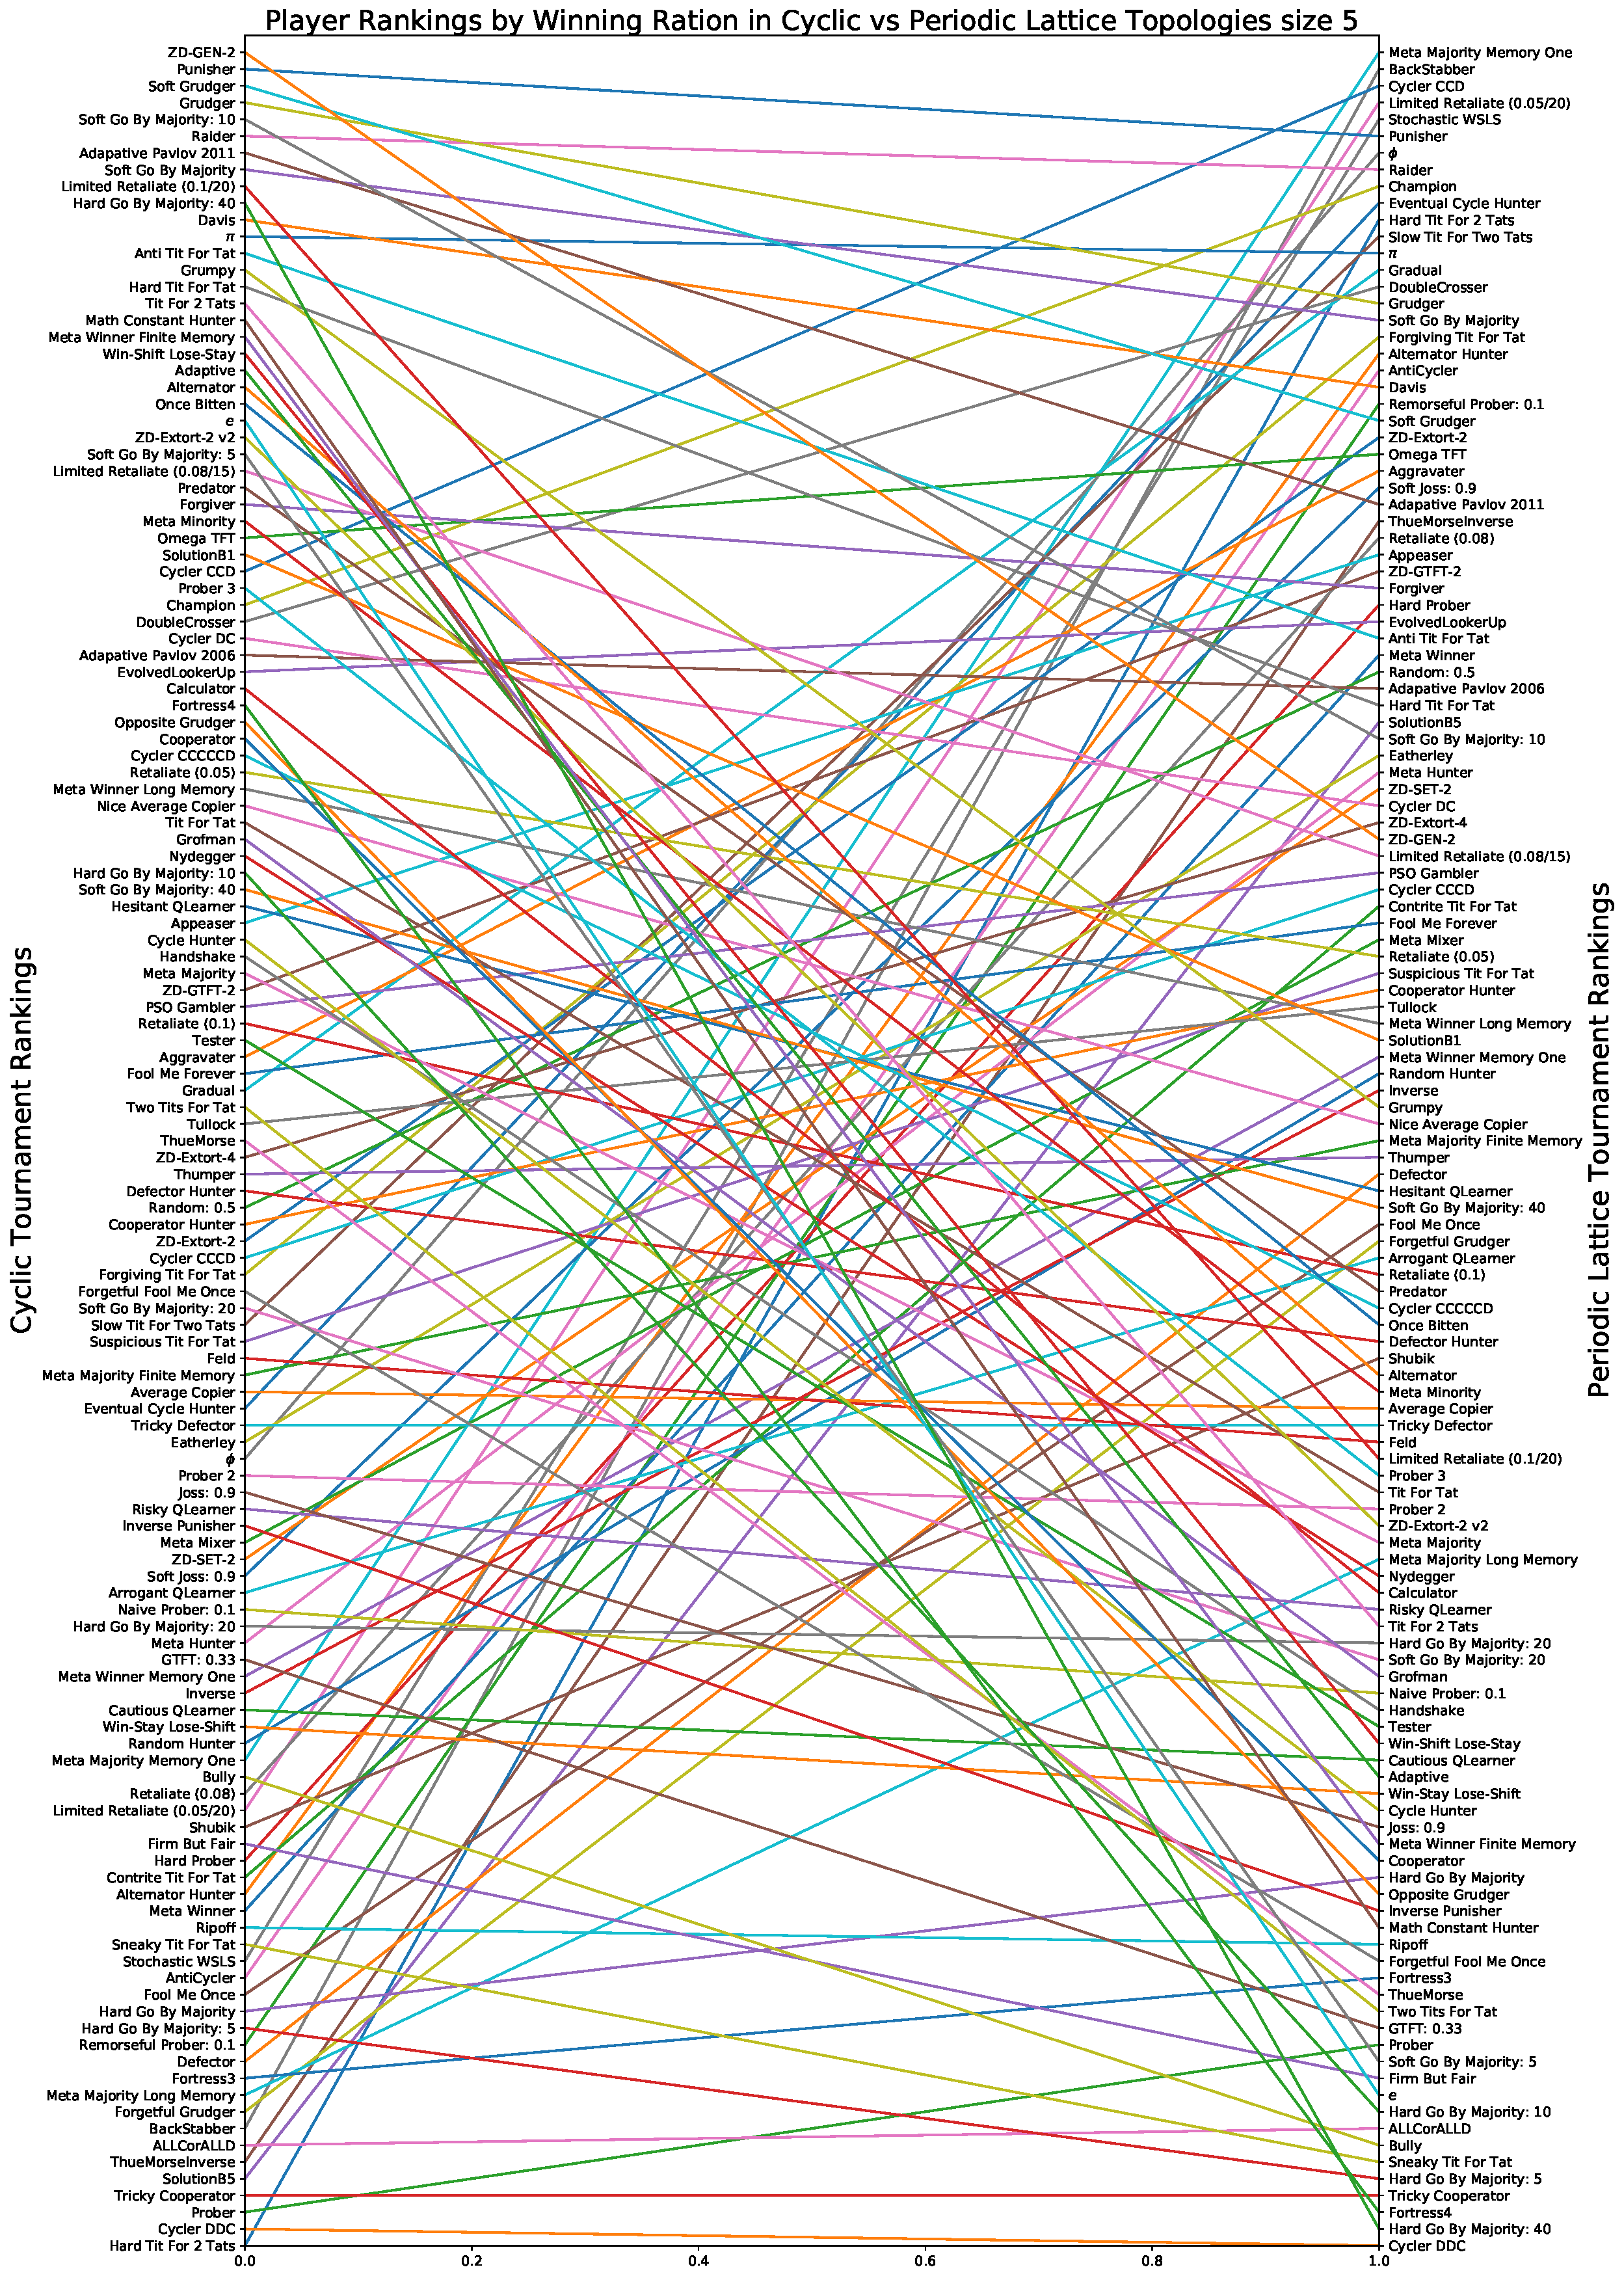
\includegraphics[width=\linewidth]{chapter-three/lines-cyclic-lattice-5.pdf}
  \caption{Cyclic vs Periodic Lattice Topologies Size 5.}
  \label{fig:winning-rankings-five-c-l}
\end{figure}

\begin{figure}[H]
\centering
    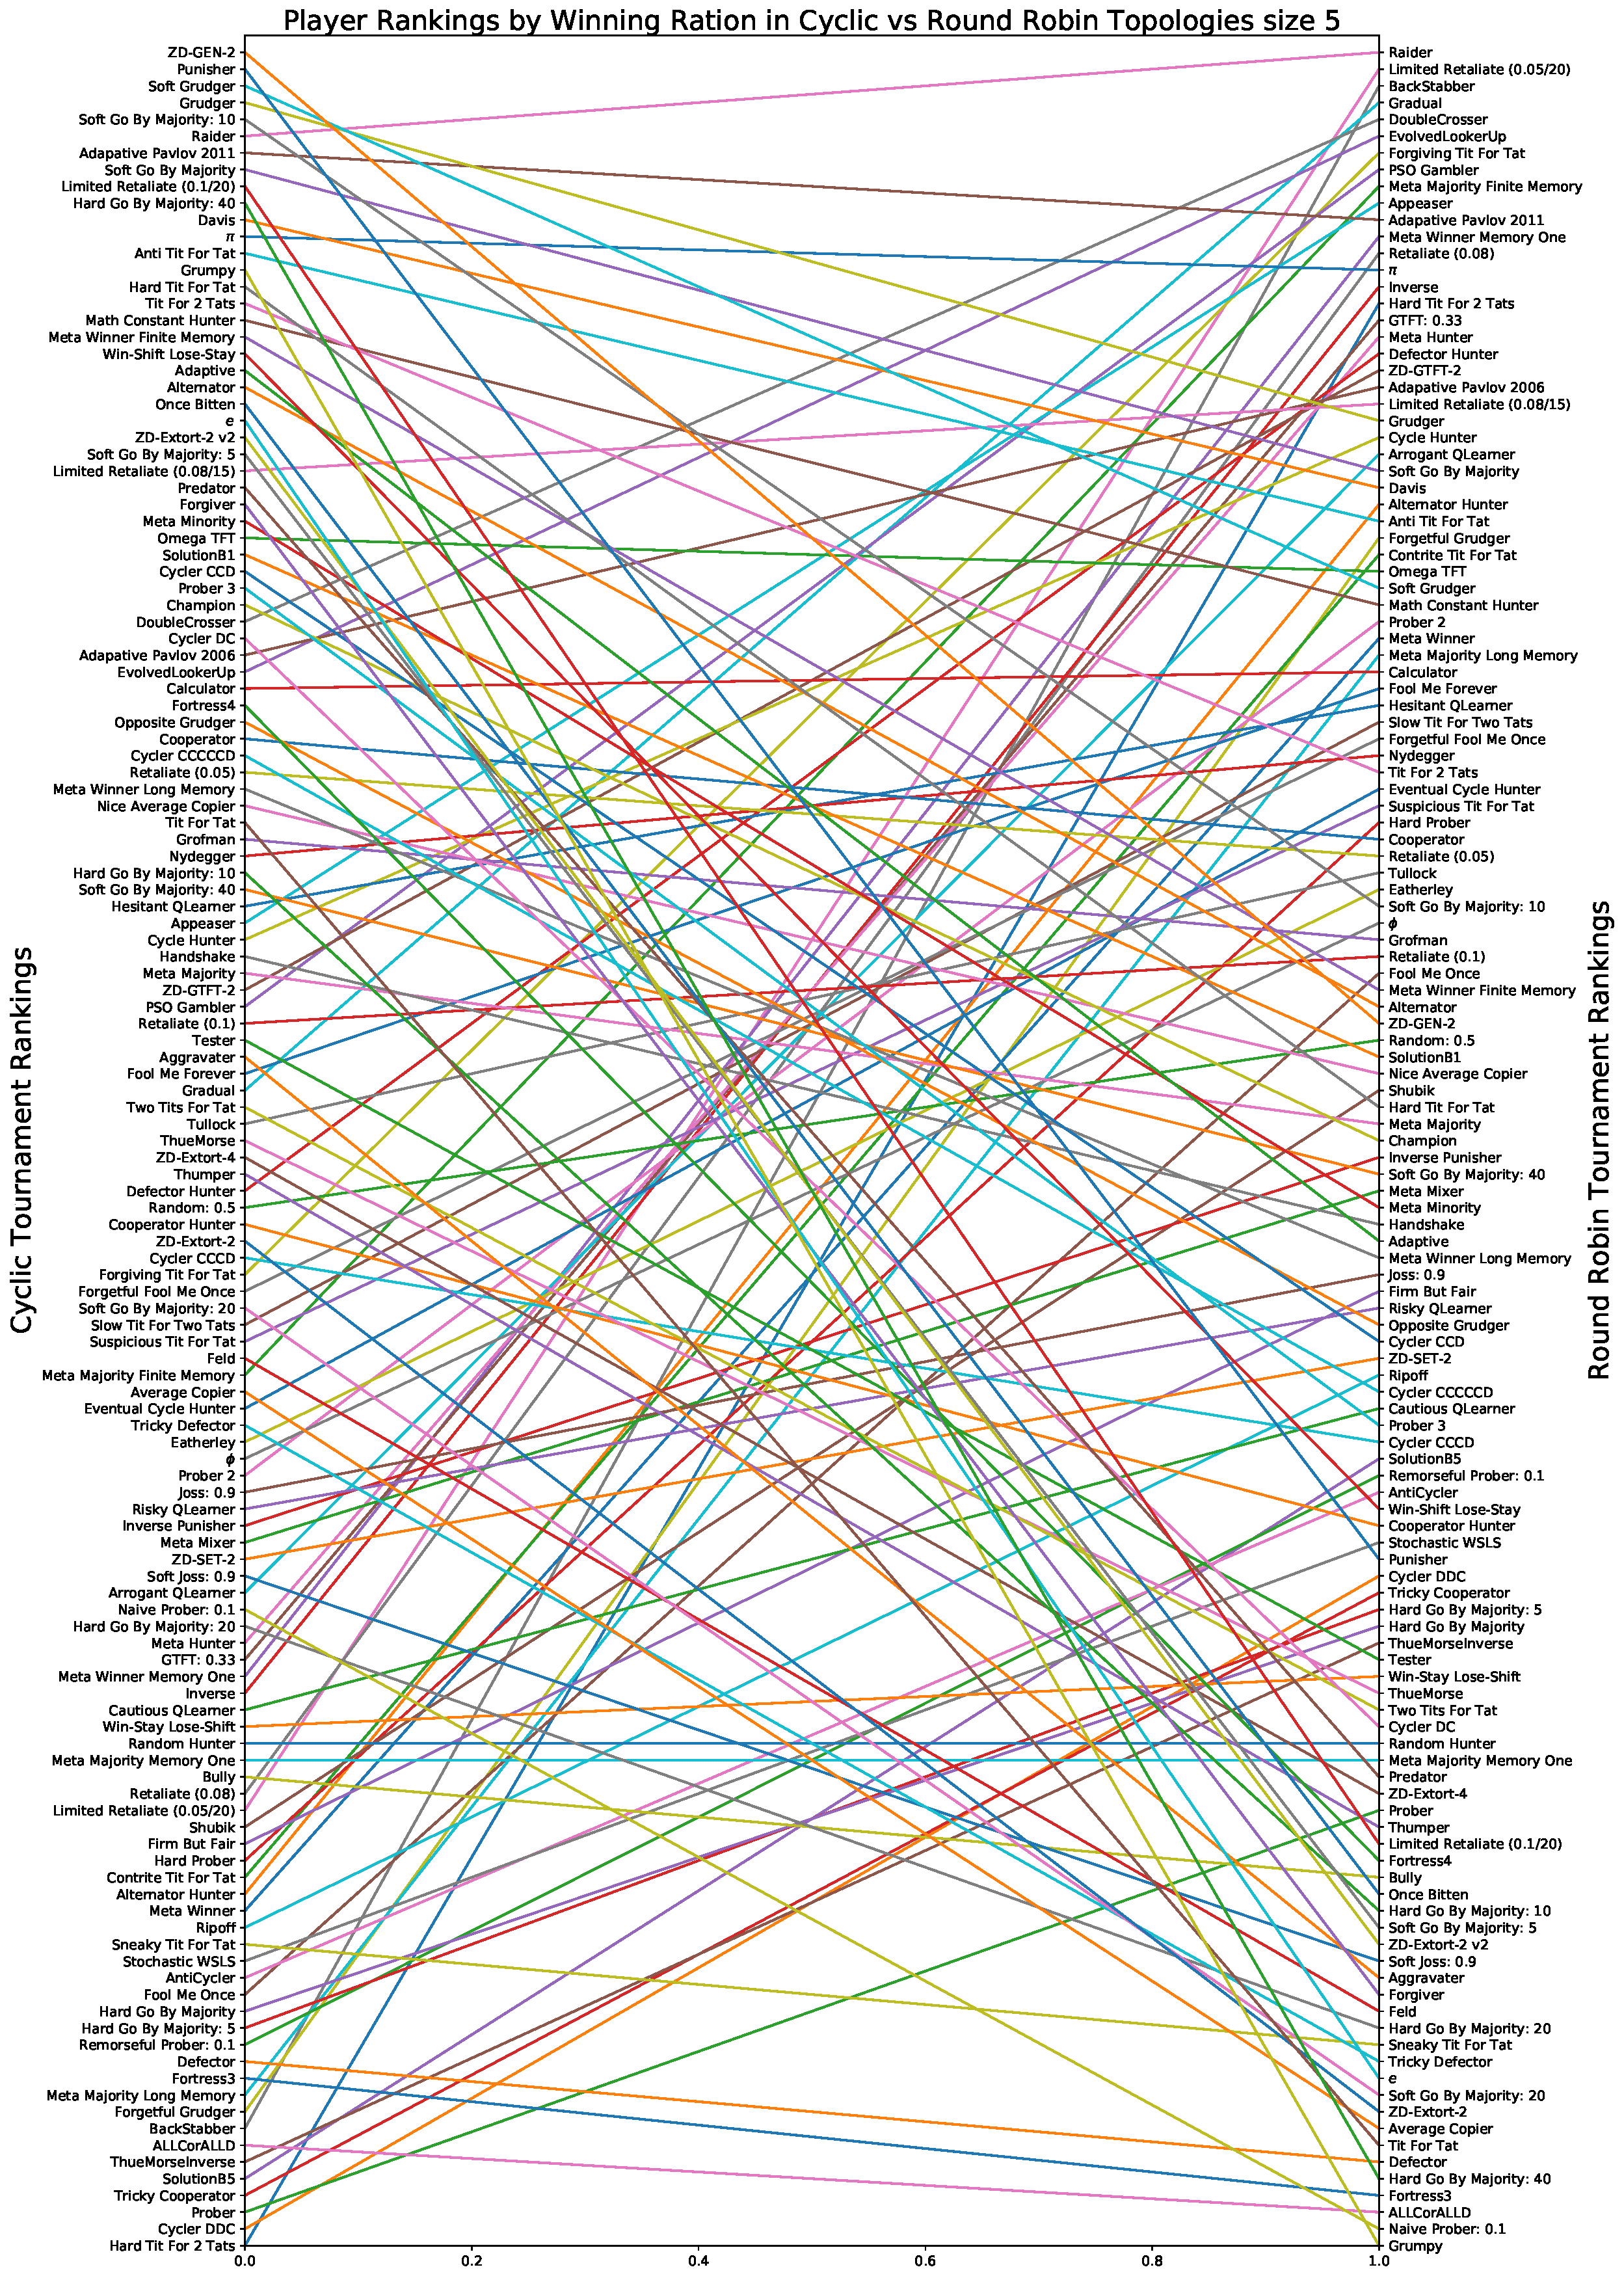
\includegraphics[width=\linewidth]{chapter-three/lines-cyclic-round-robin-5.pdf}\
\caption{Cyclic vs Round Robin Topologies Size 5.}
\label{fig:winning-rankings-five-c-r}
\end{figure}

\begin{figure}[H]
\centering
    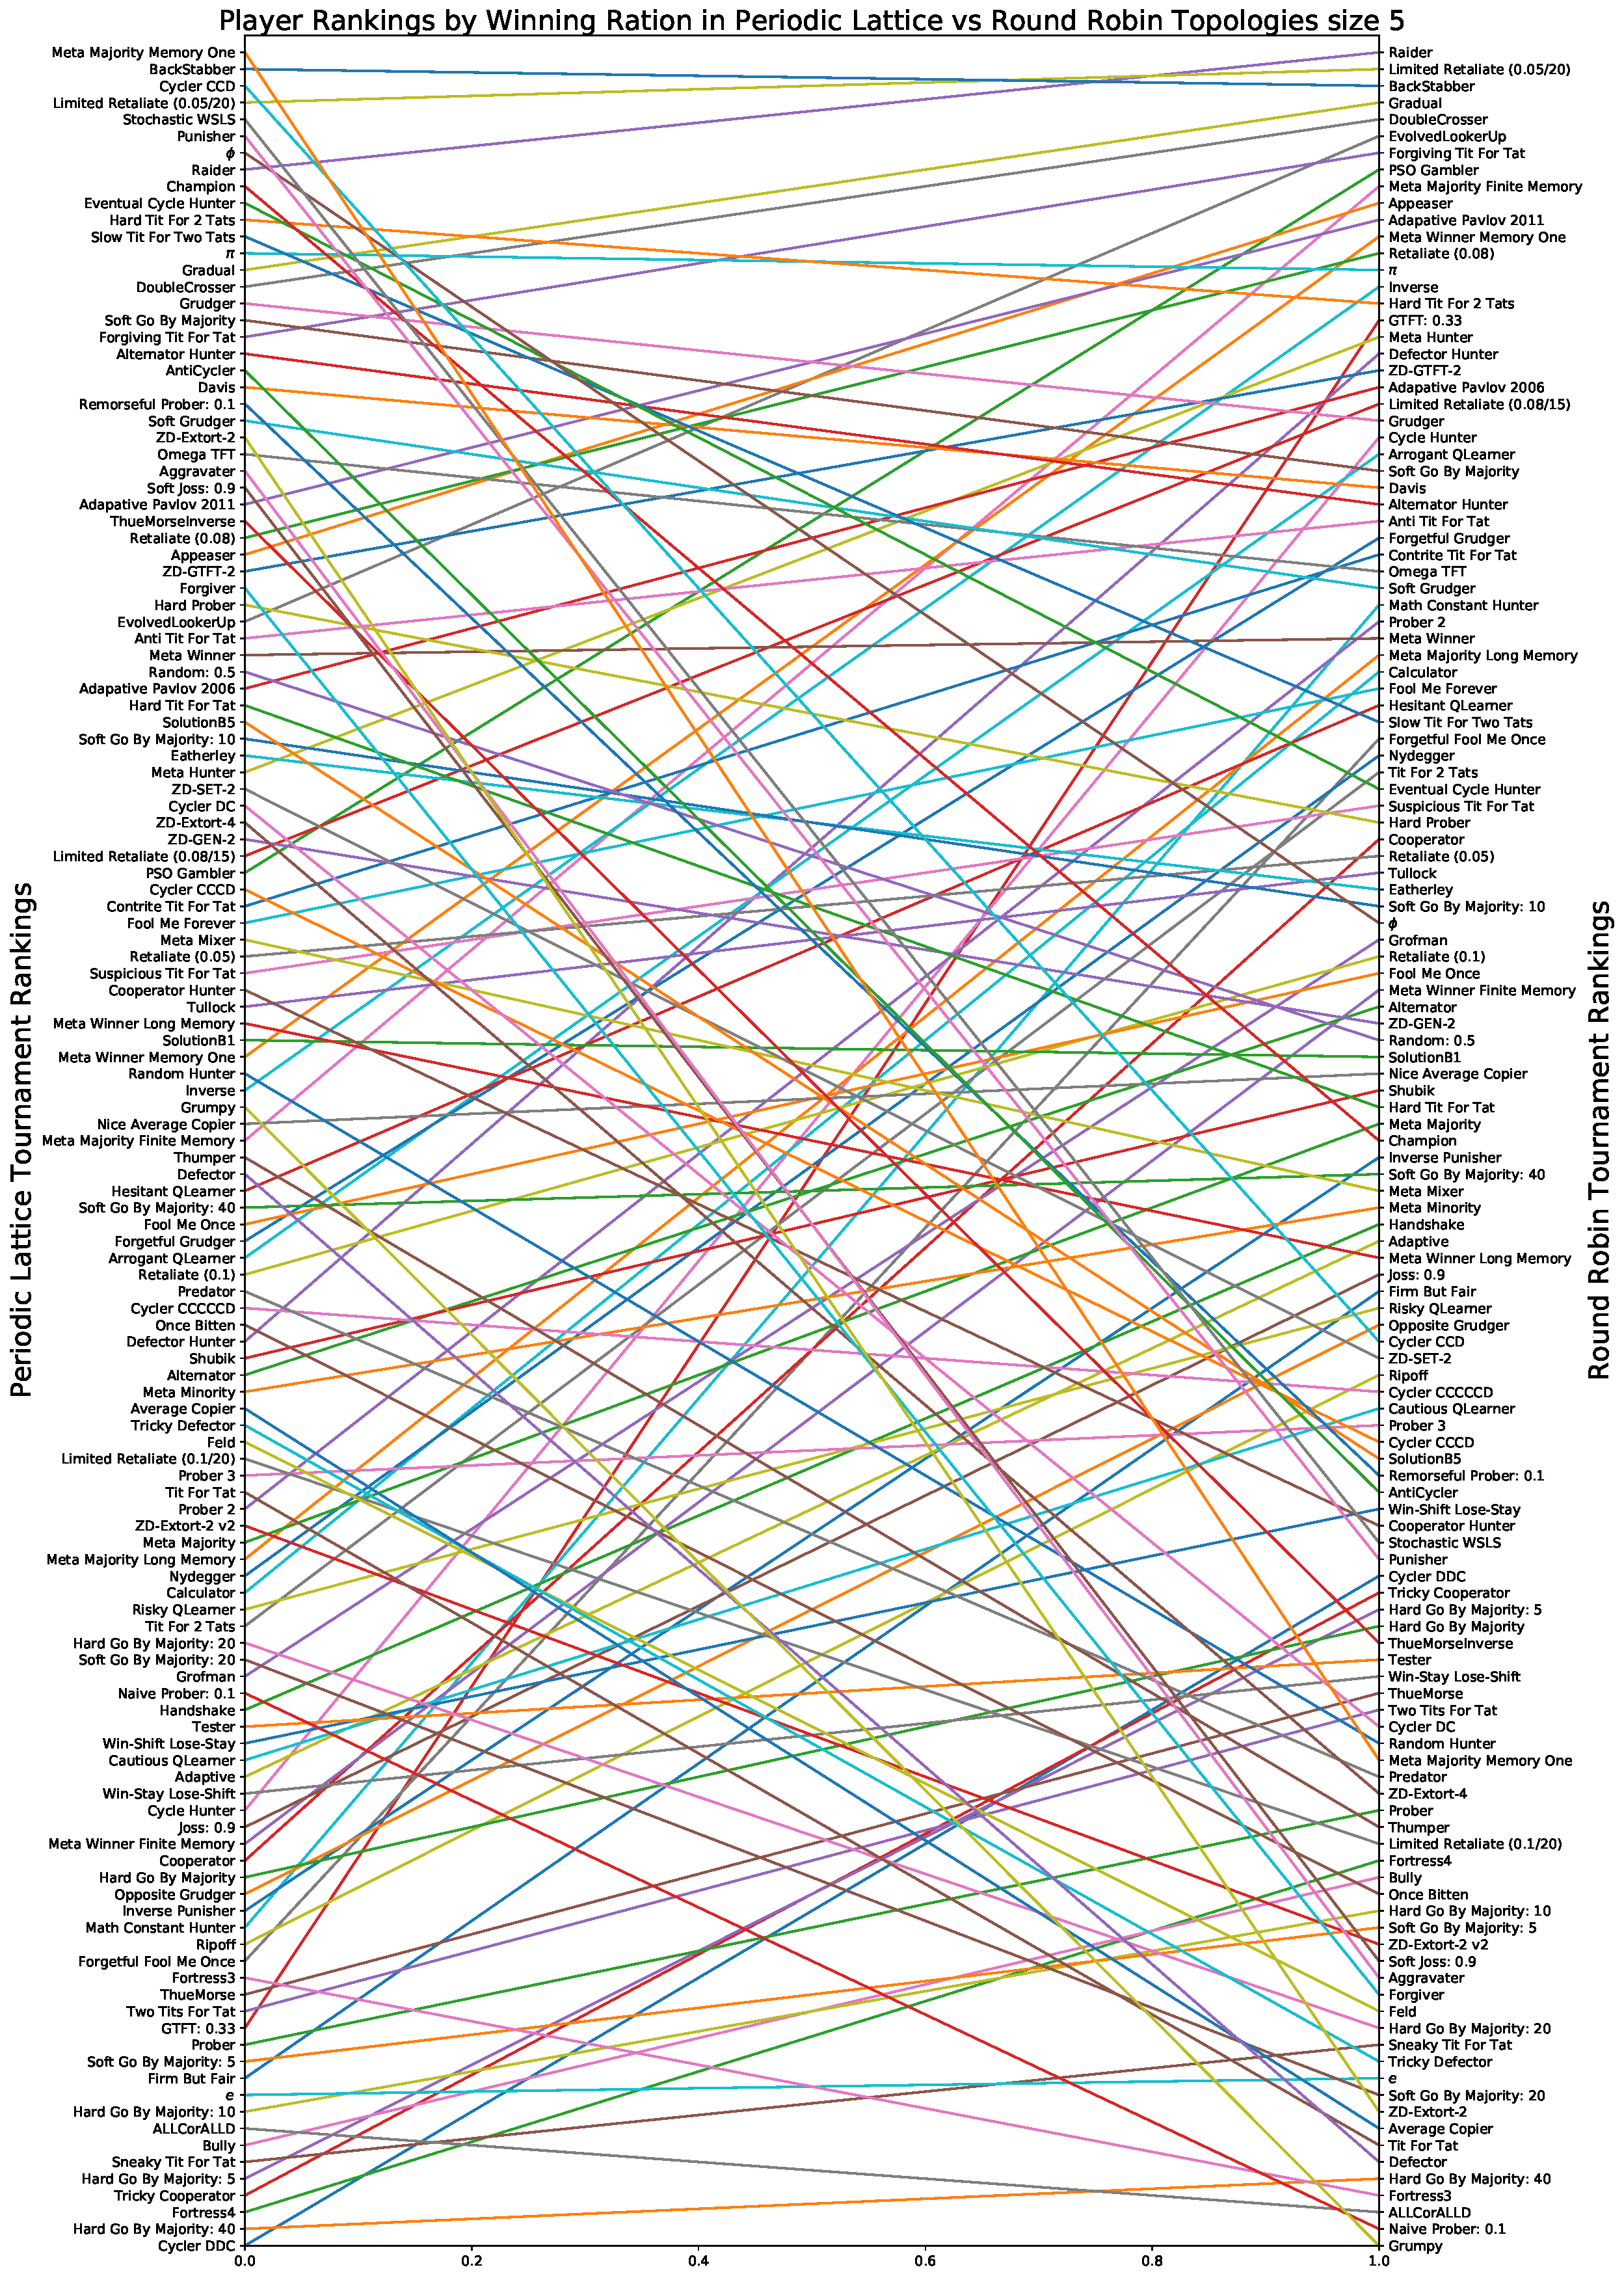
\includegraphics[width=\linewidth]{chapter-three/lines-lattice-round-robin-5.pdf}\
\caption{Periodic Lattice vs Round
         Robin Topologies Size 5.}
\label{fig:winning-rankings-five-l-r}
\end{figure}

\begin{figure}[H]
\centering
    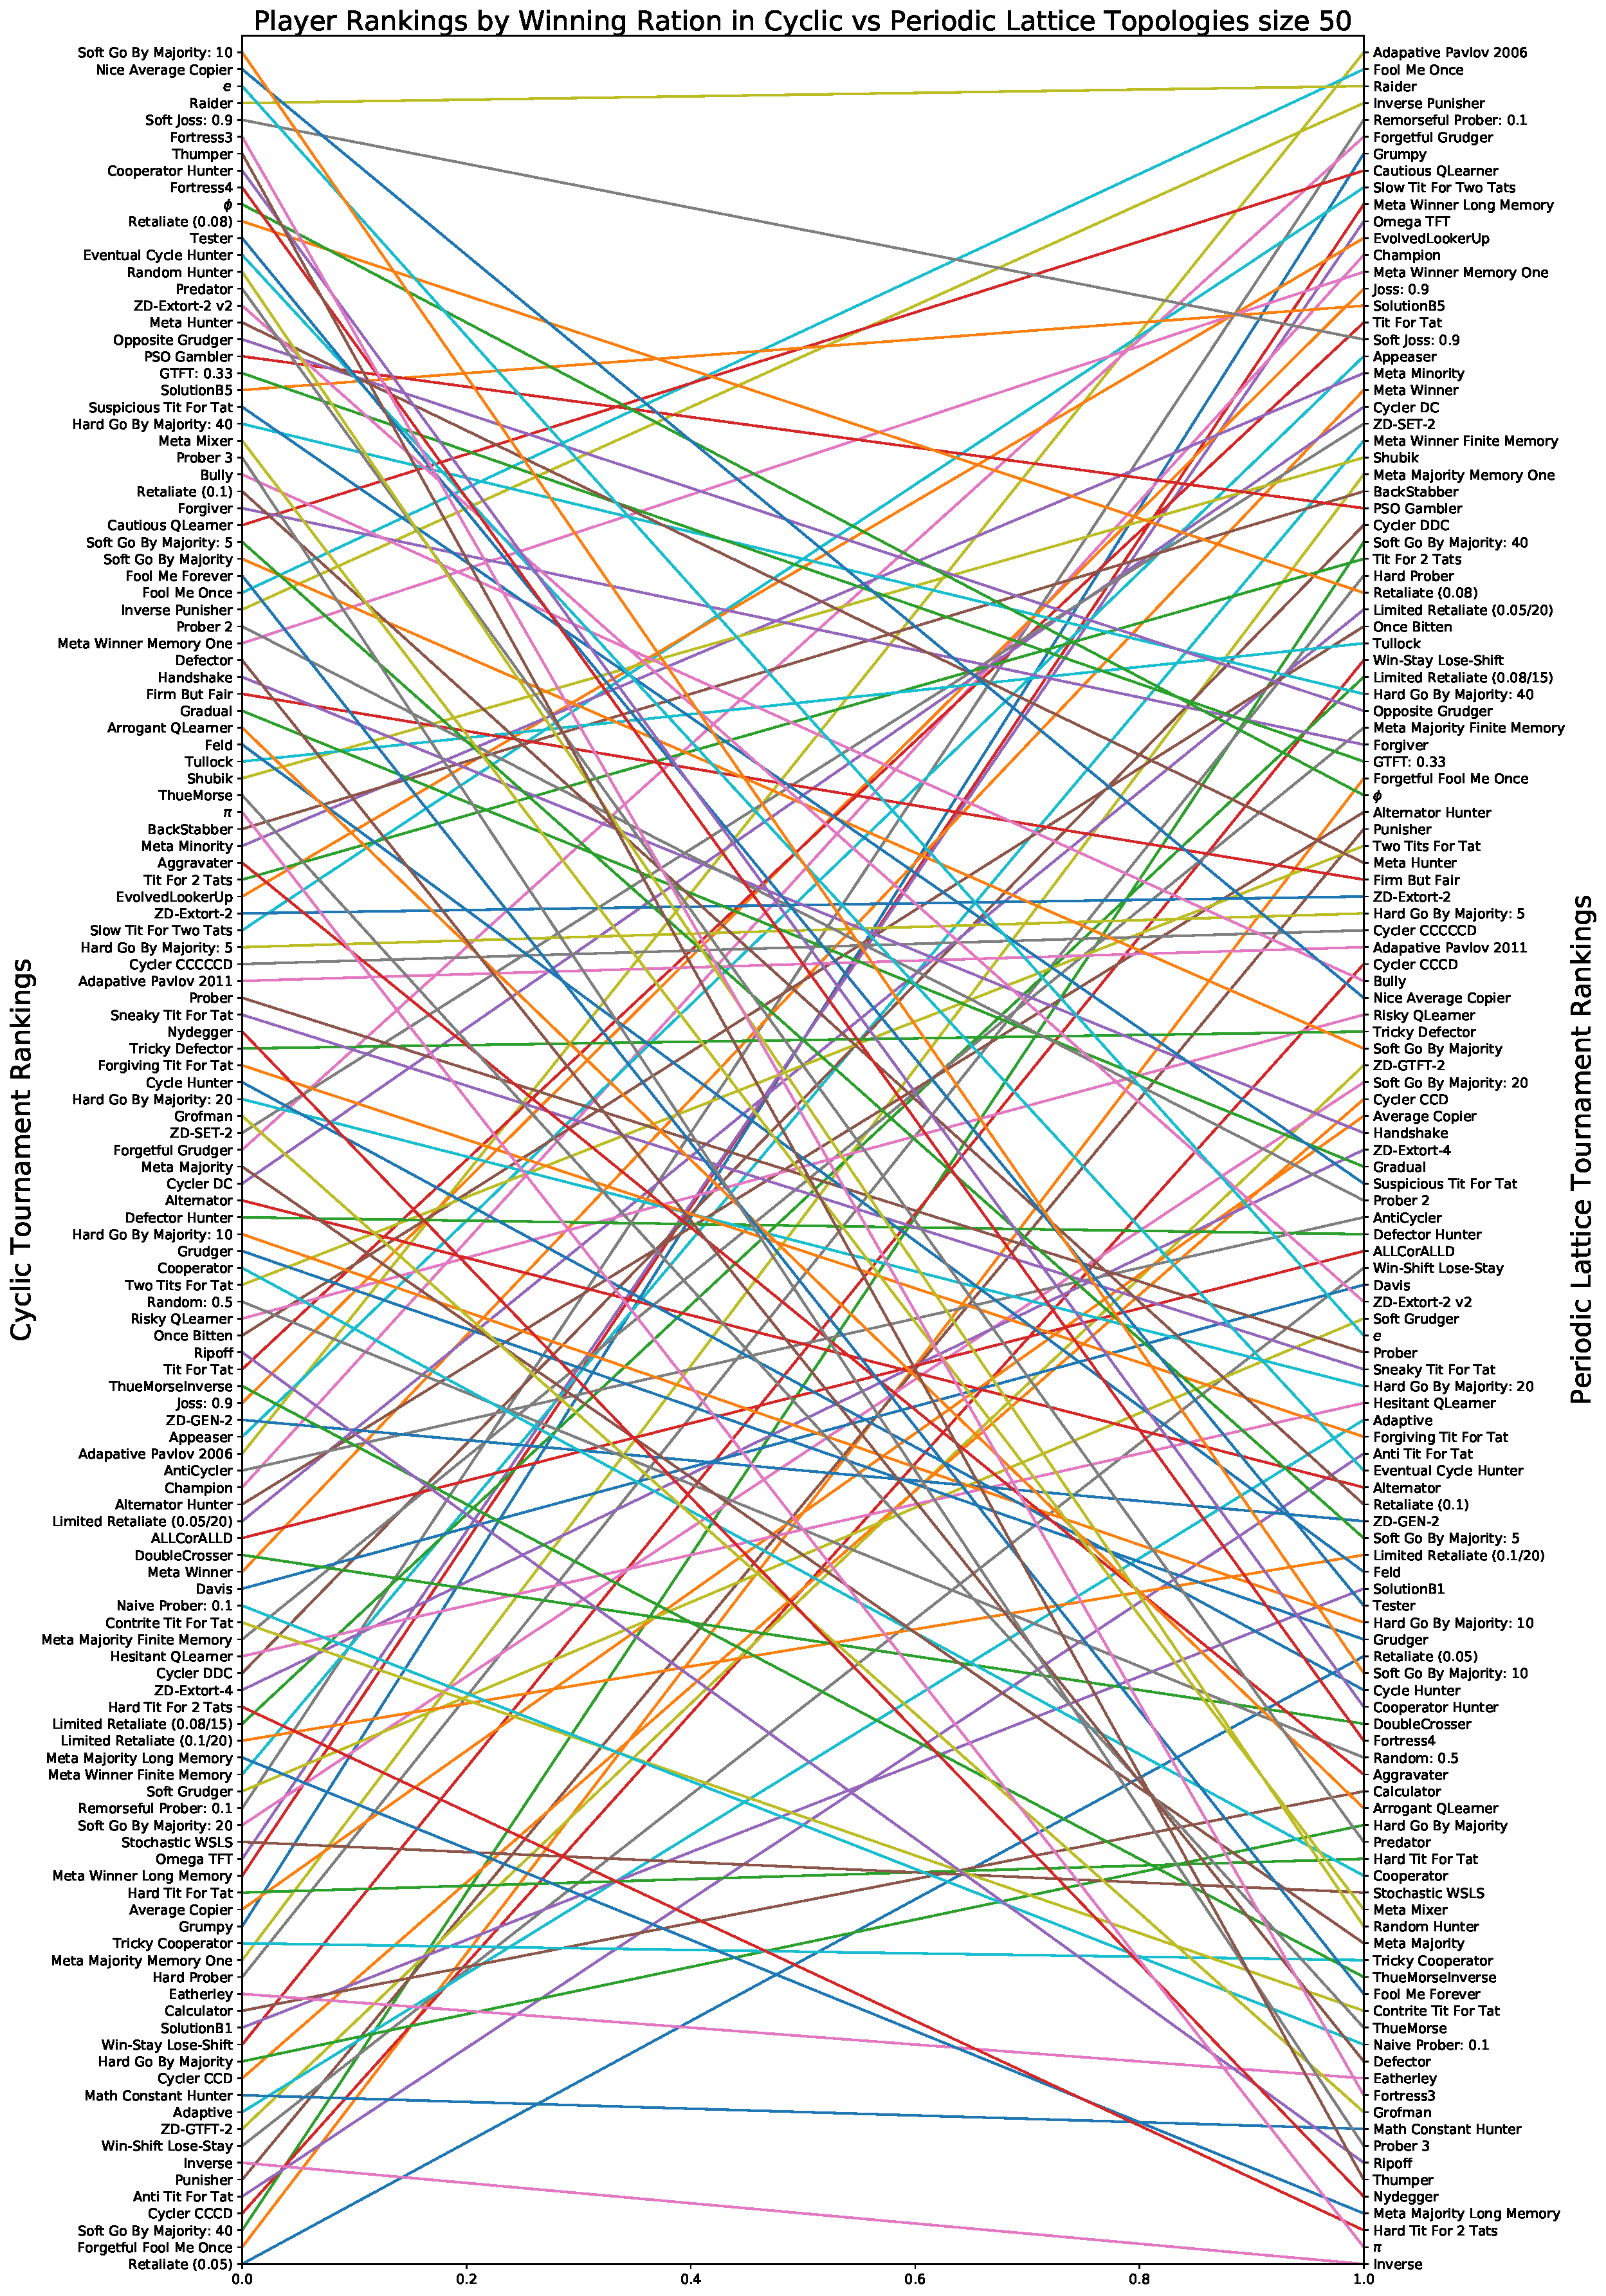
\includegraphics[width=\linewidth]{chapter-three/lines-cyclic-lattice-50.pdf}
\caption{Cyclic vs Periodic Lattice Topologies Size 50.}
\label{fig:winning-rankings-fifty-c-l}
\end{figure}

\begin{figure}[H]
\centering
    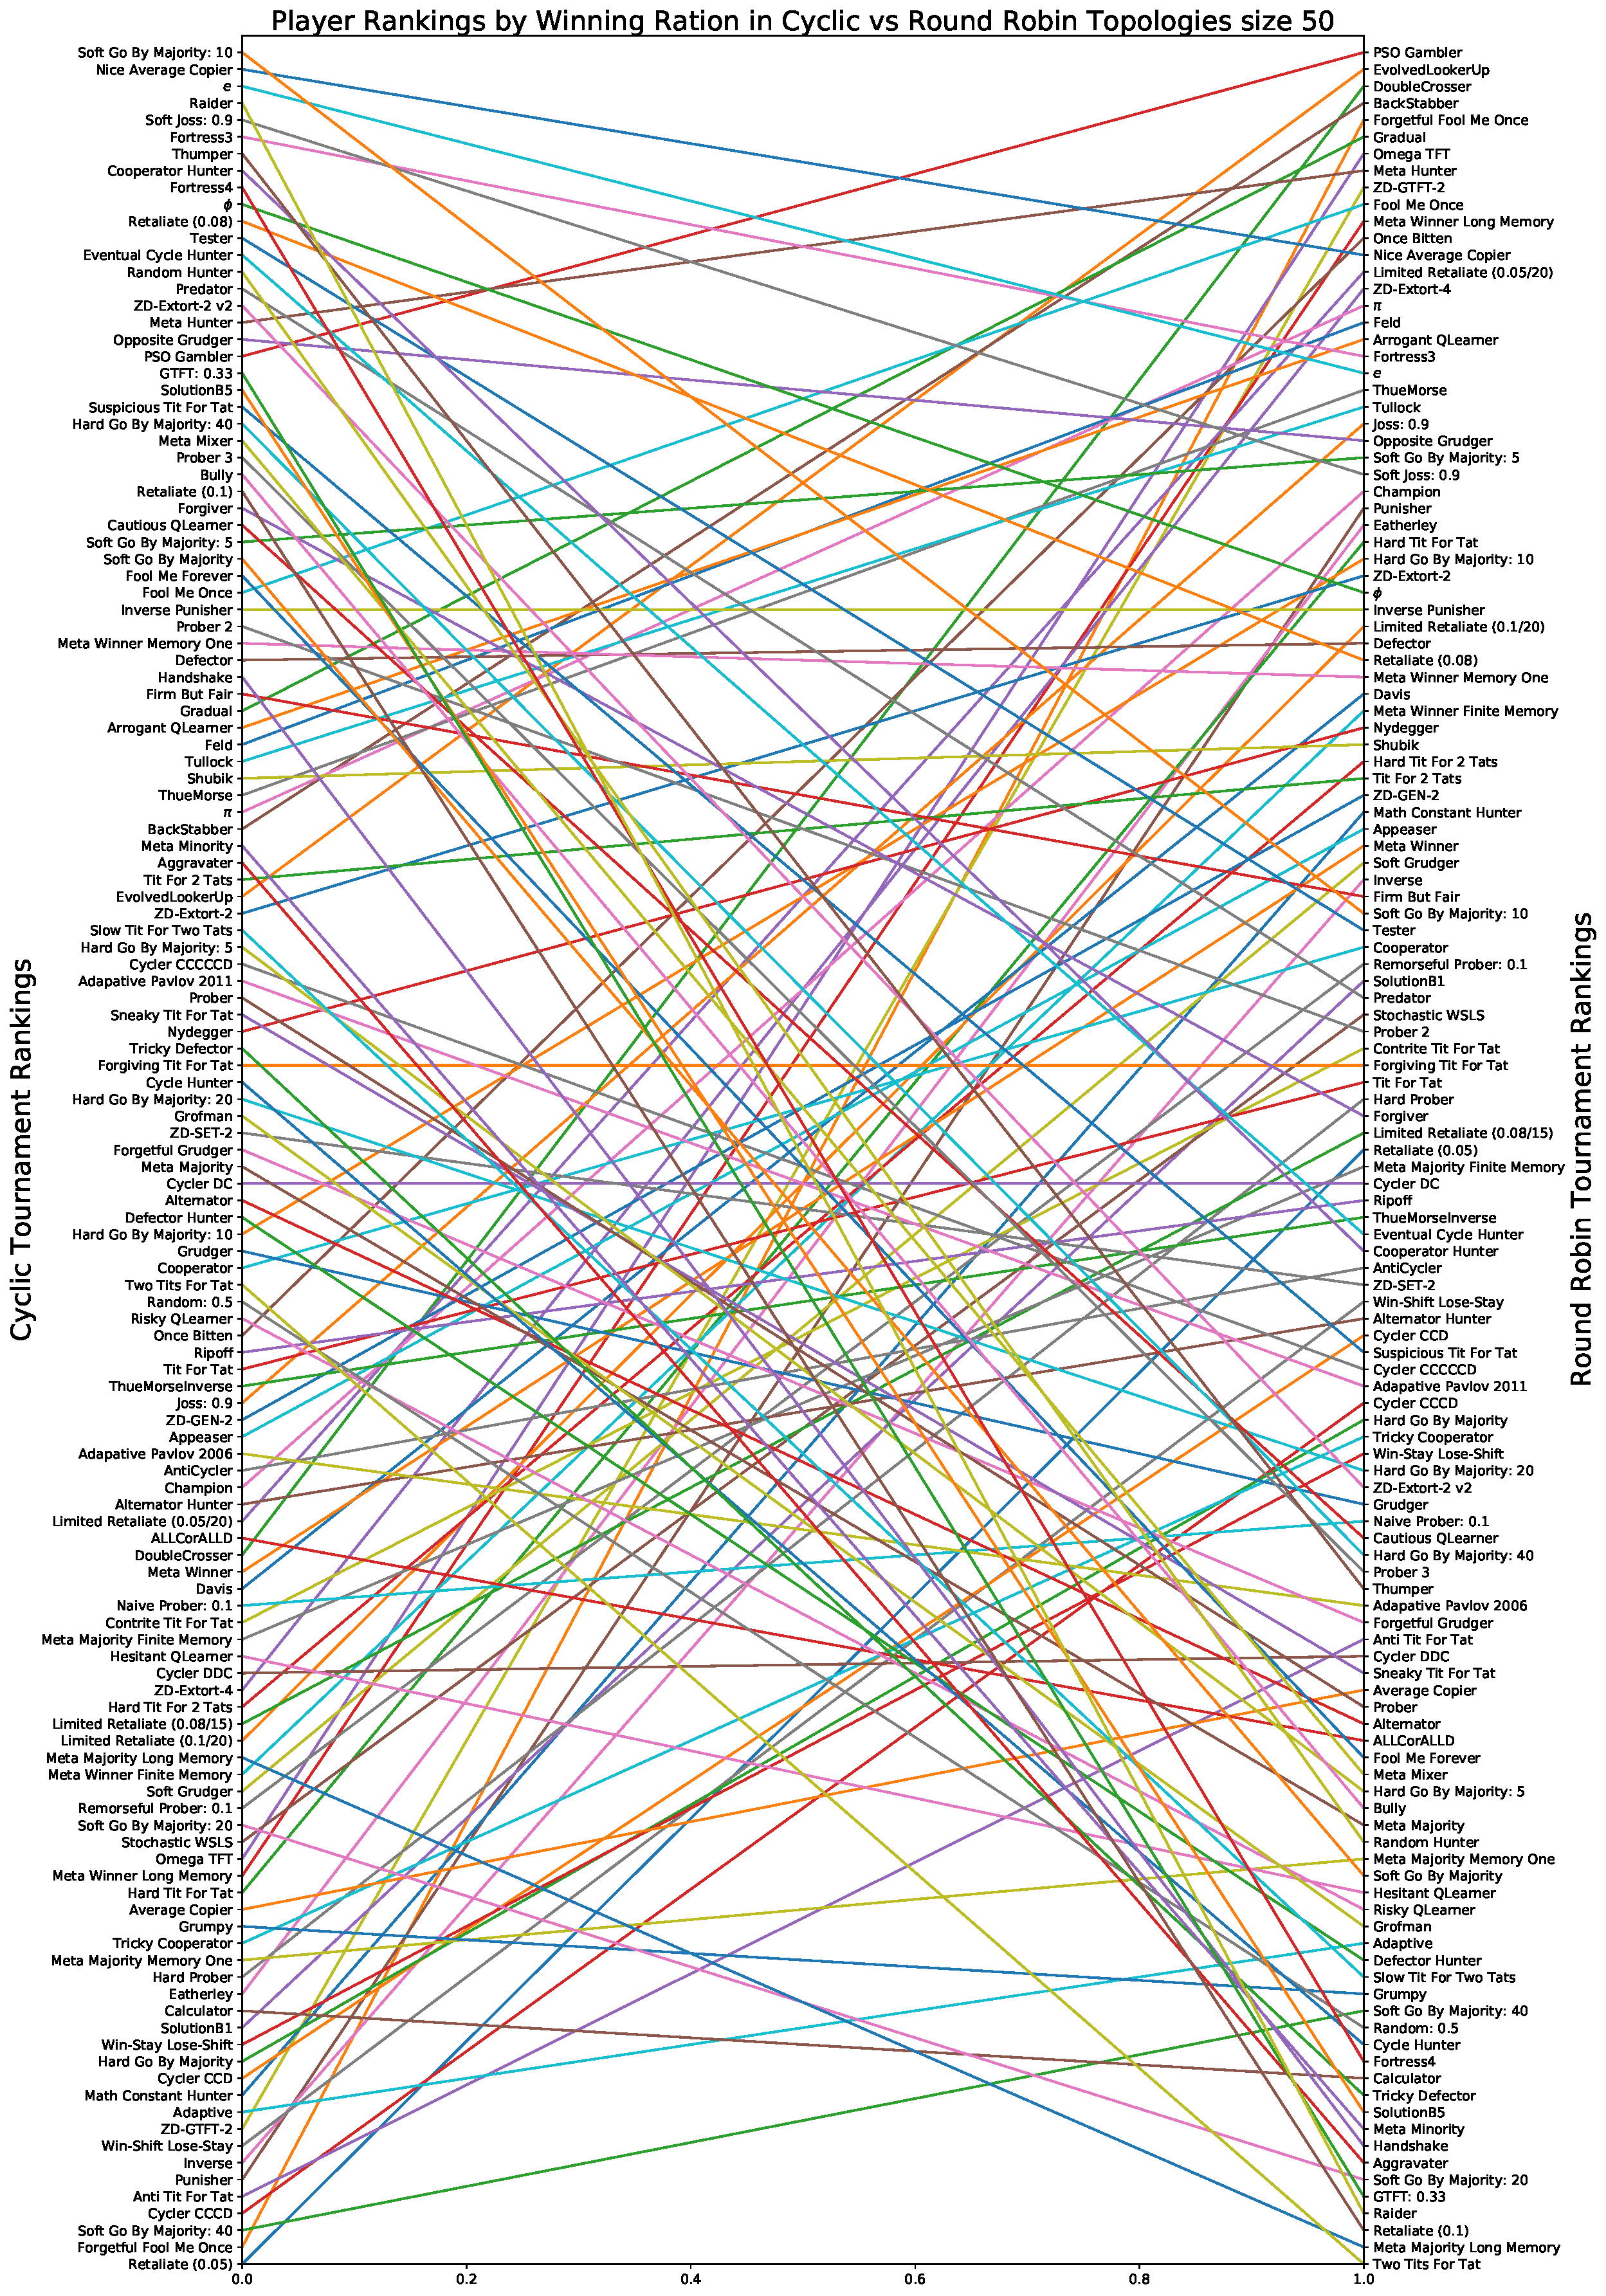
\includegraphics[width=\linewidth]{chapter-three/lines-cyclic-round-robin-50.pdf}
\caption{Cyclic vs Round Robin Topologies Size 50.}
\label{fig:winning-rankings-fifty-c-r}
\end{figure}

\begin{figure}[H]
\centering
    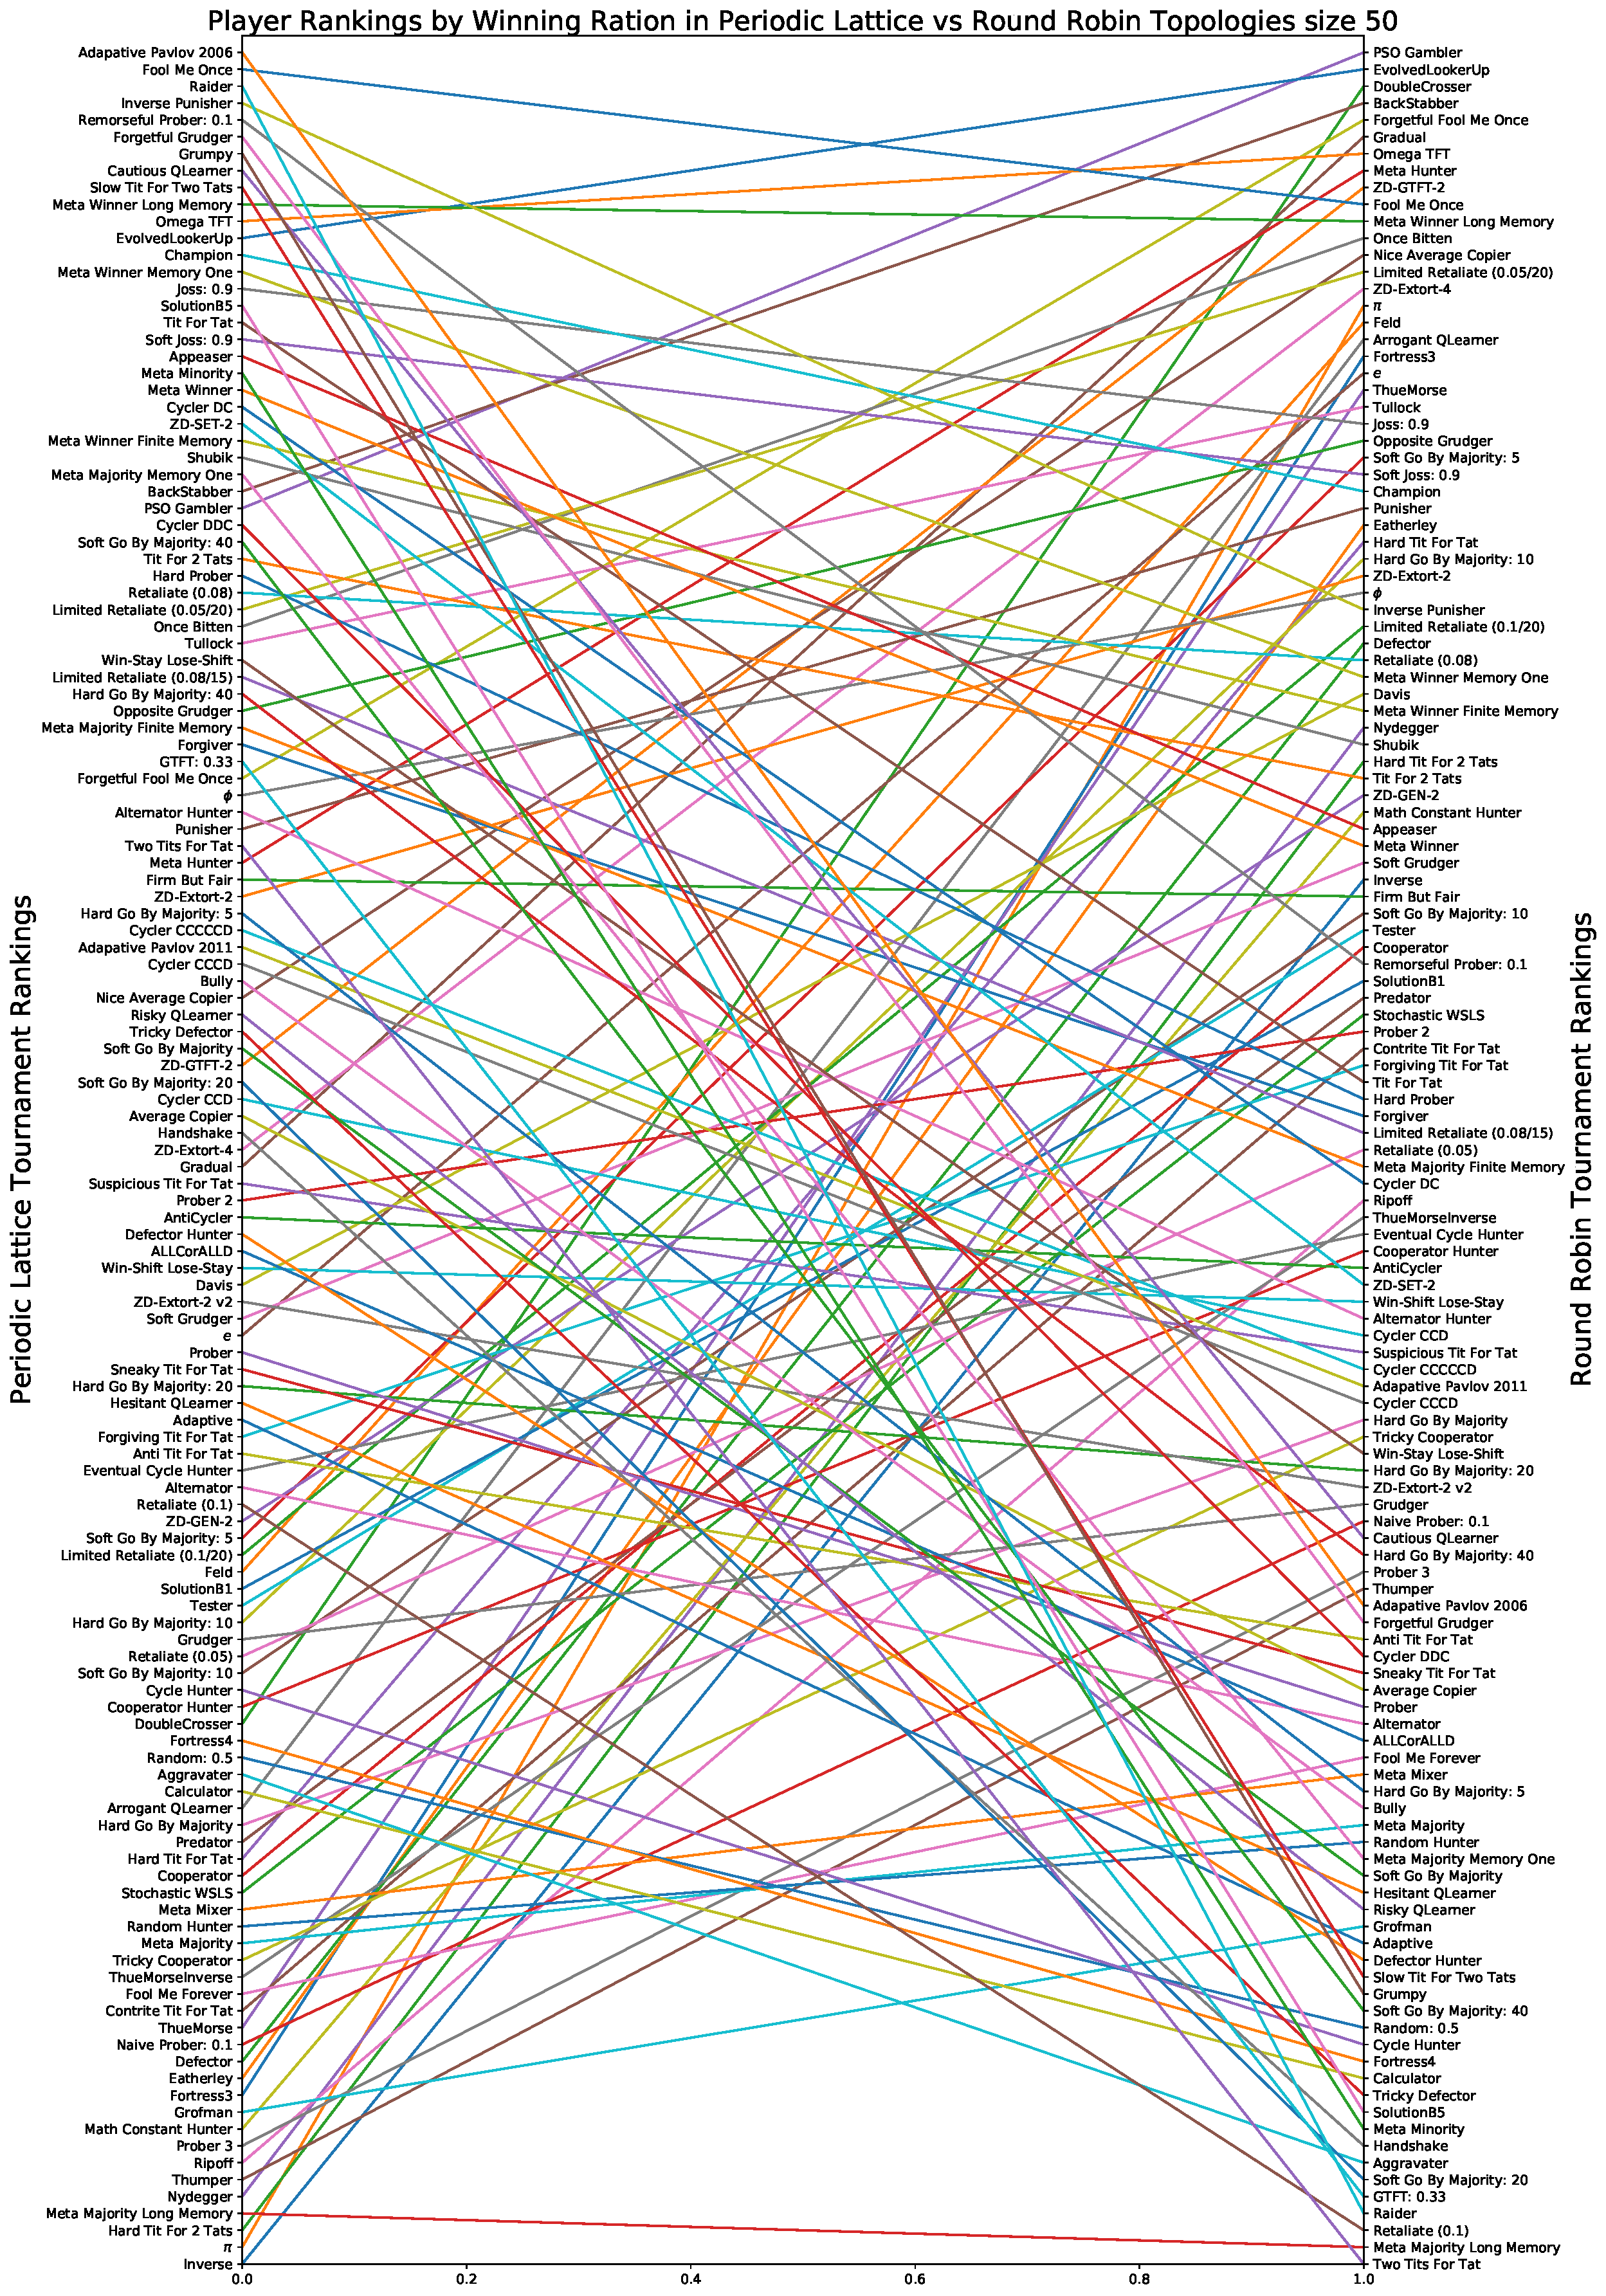
\includegraphics[width=\linewidth]{chapter-three/lines-lattice-round-robin-50.pdf}
\caption{Periodic Lattice vs Round
             Robin Topologies Size 50.}
             \label{fig:winning-rankings-fifty-l-r}
\end{figure}

The strategies can be classified based on the number of tournament
participations. For tournament size 5, 9 classes have been created for
the cyclic and the periodic lattice topologies, [10, 20, 30, 40, 50, 60, 70, 80, 90].
For tournament
size 50, [270, 280, 290, 310, 320, 330, 340, 350, 360, 370, 380, 390, 400, 410,
420, 430, 440, 450, 460, 470, 570]. Round robin topology
experiments were classified as [1, 2, 3, 4, 5, 6, 7, 8, 9] and
[27, 28, 29, 31, 32, 33, 34, 35, 36, 37, 38, 39, 40, 41, 42, 43, 44, 45, 46, 47, 57],
respectively. The winning ratios were plotted against participation number
in Figures~\ref{fig:winning-ratio-participations-five} and~\ref{fig:winning-ratio-participations-fifty}.
An ANOVA analysis was used to analyze the importance of the
differences in the winning ratios among the participating groups.

The anova results, for a tournament of size equal to 5,
indicate that for the topologies cyclic and periodic lattice the difference
of ratios between the participations groups is significant (\(p\) values
are lower that 0.05). Shown in Figure~\ref{fig:winning-ratio-participations-five},
are violin plots of the winning ratio against number of participations. A positive
trend can be spotted for the lattice and cyclic topology. For the round robin
topology, the anova test suggests no correlation between ratio and participating.

Equivalently, in ~\ref{fig:winning-ratio-participations-fifty}, violin plots for
tournament size 50 are displayed.  In the anova results from Table~\ref{anova-size-fifty},
\(p\) values of a round robin and of a cyclic topology are greater that 0.05.
Compared to that of a lattice, where the \(p\) values is below 0.05 and, therefore,
there is a statistically significant difference.
Thus, participating number affects the winning ratios for only two out of the six
experiments. The specific groups that different are not clear.
Post-hoc analysis could be performed but will not be considered here.

\begin{table}[H]
\centering
\begin{adjustbox}{width=0.5\textwidth}
\small
\begin{tabular}{|l|l|l|l|}
\hline
Topology         & \multicolumn{3}{l|}{Anova results tournament size 5} \\ \hline
                 & Sum of Squares      & F ratio     & \(p\) value          \\ \hline
Cyclic           & 0.41                & 33.83       & 6.379416e-09     \\ \hline
Periodic Lattice & 0.04                & 4.24        & 0.039            \\ \hline
Round Robin      & 0.008               & 0.18        & 0.66             \\ \hline
\end{tabular}
\end{adjustbox}
\caption{Anova results tournament size 5}
\label{anova-size-five}
\end{table}

\begin{table}[H]
\centering
\begin{adjustbox}{width=0.5\textwidth}
\small
\begin{tabular}{|l|l|l|l|}
\hline
Topology         & \multicolumn{3}{l|}{Anova results tournament size 5} \\ \hline
                 & Sum of Squares     & F ratio     & \(p\) value           \\ \hline
Cyclic           & 0.000056           & 1.12        & 0.28              \\ \hline
Periodic Lattice & 0.045              & 1110.45     & 7.777650e-241     \\ \hline
Round Robin      & 0.00098            & 0.10        & 0.74              \\ \hline
\end{tabular}
\end{adjustbox}
\caption{Anova results tournament size 50}
\label{anova-size-fifty}
\end{table}

\begin{figure}[H]
\centering

    \begin{subfigure}[t]{0.75\textwidth}
    \centering
        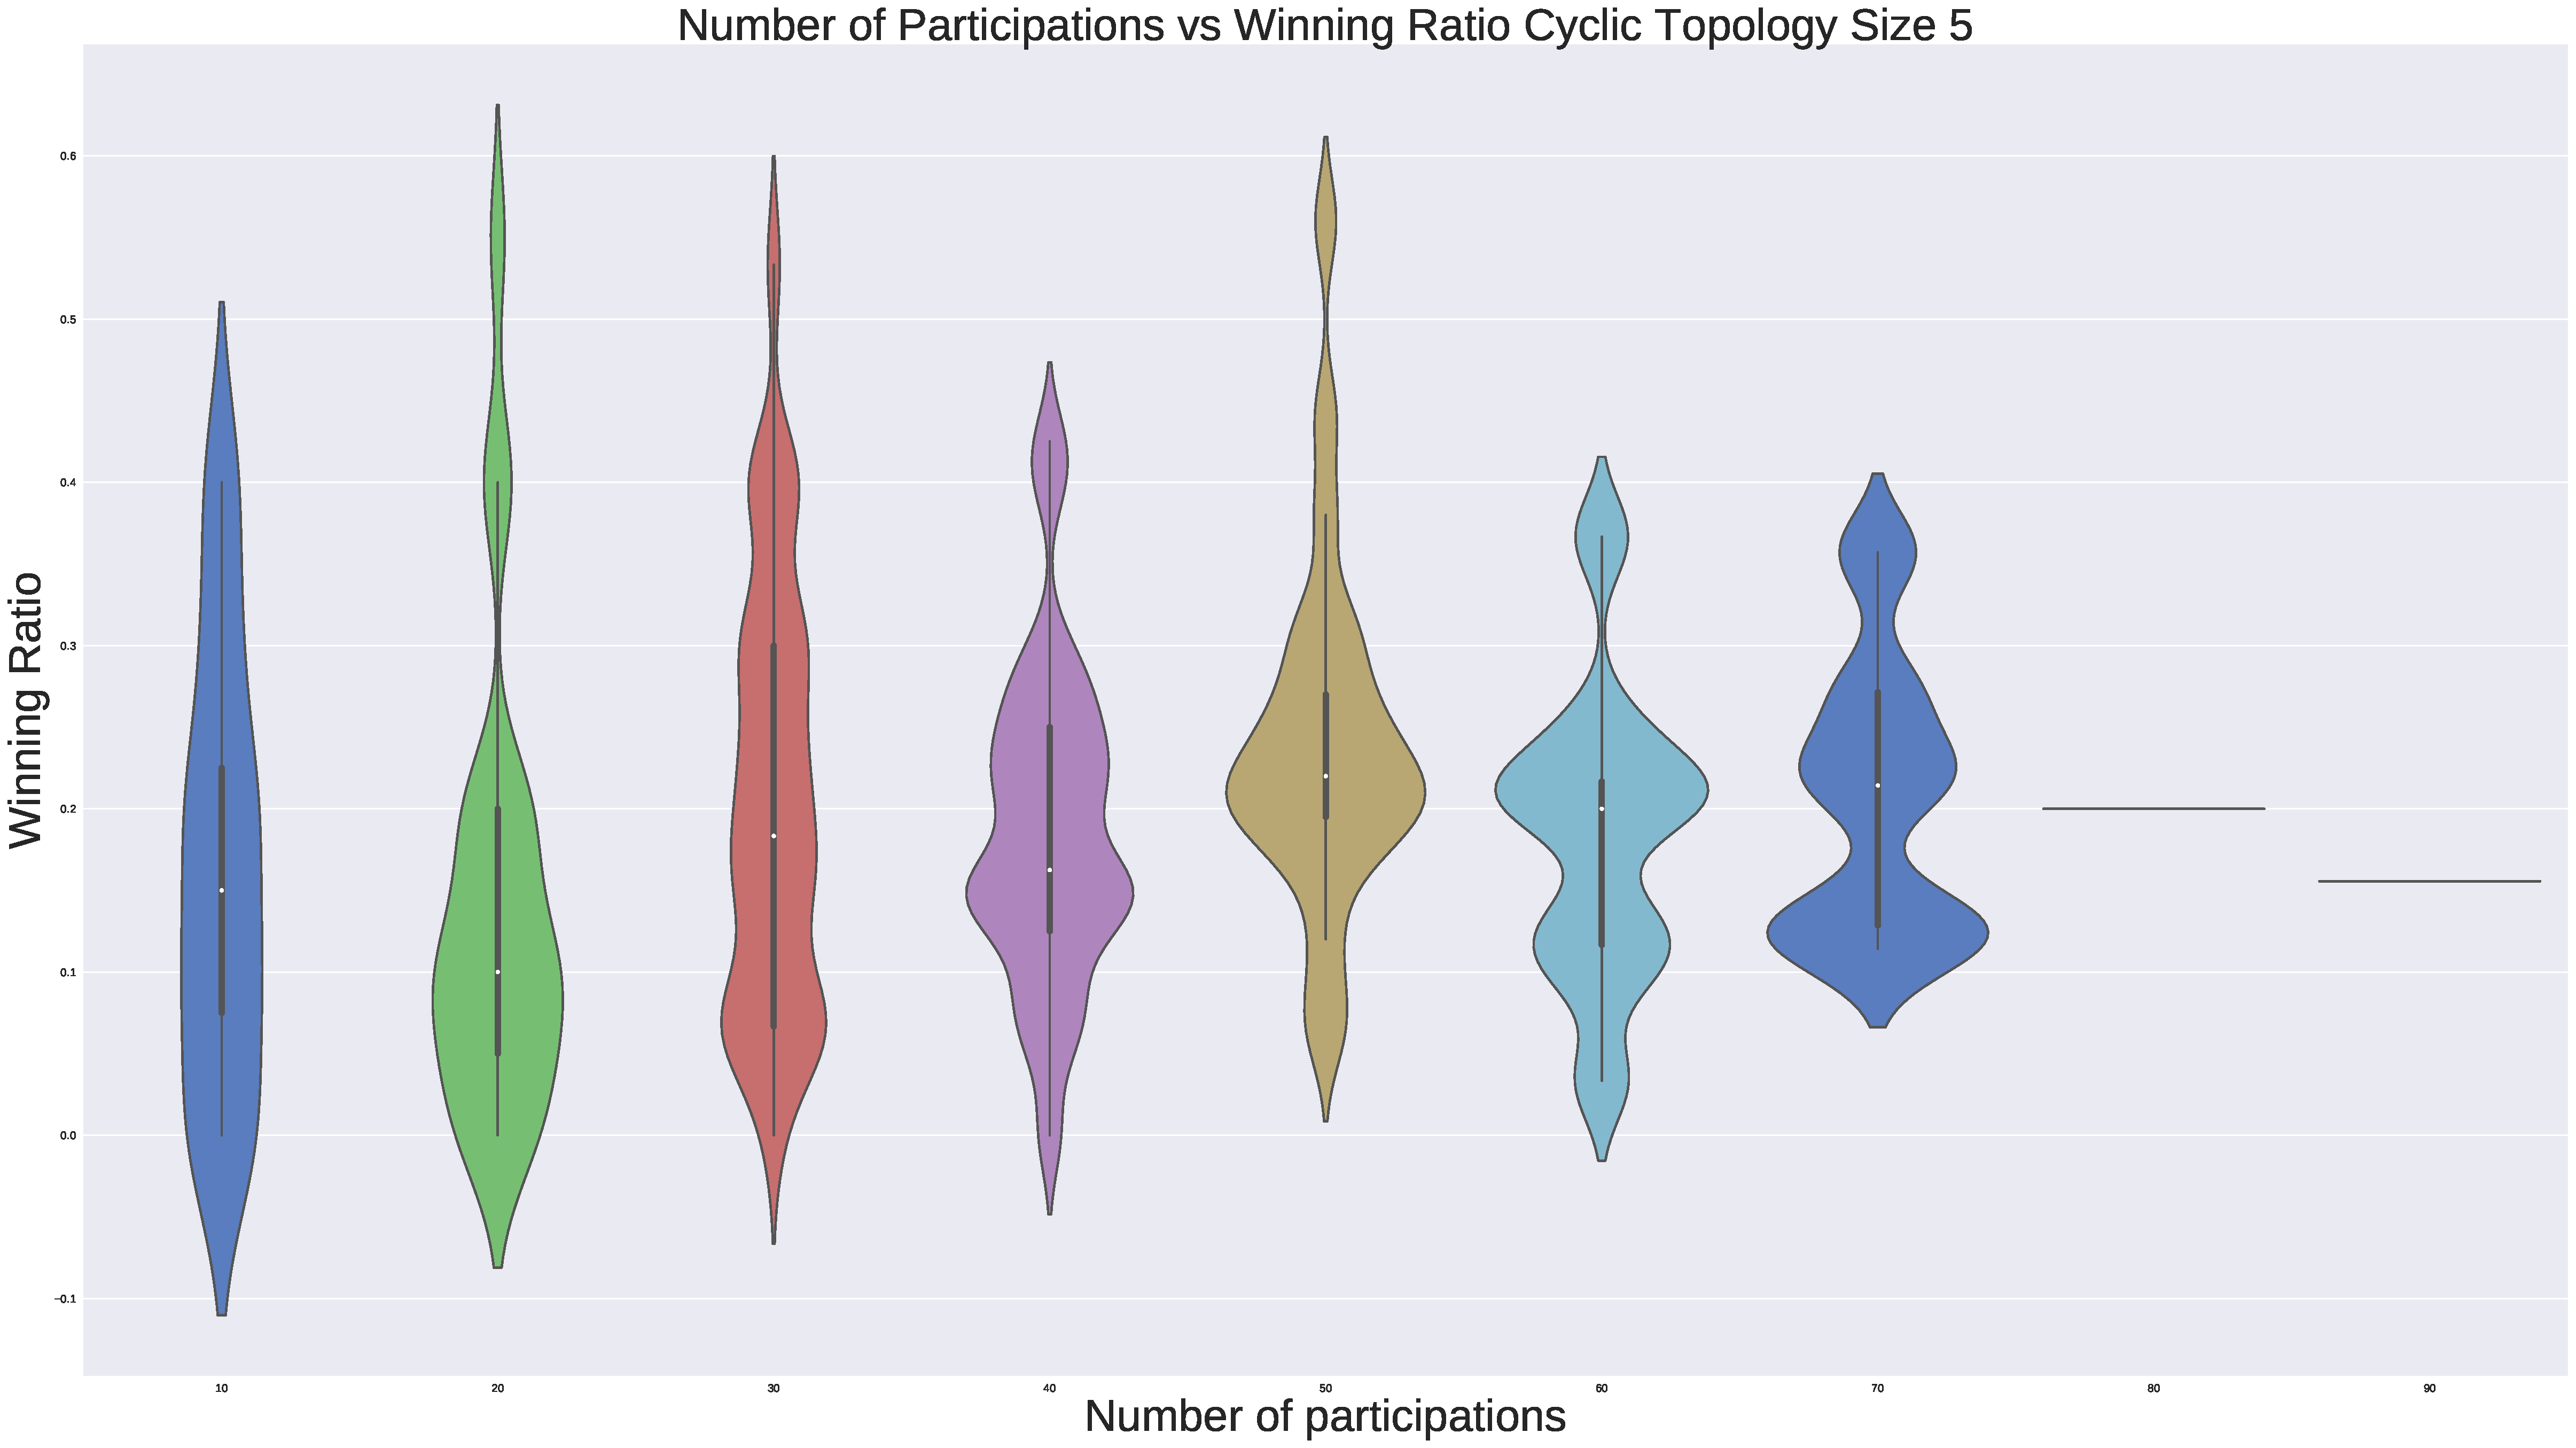
\includegraphics[width=\linewidth]{chapter-three/participation-ratio-violin-Cyclic-5.pdf}
    \caption{Winning Ratio vs Number of Participations Cyclic Tournament Size 5.}
    \end{subfigure}
\hfill
    \begin{subfigure}[t]{0.75\textwidth}\centering
    \centering
        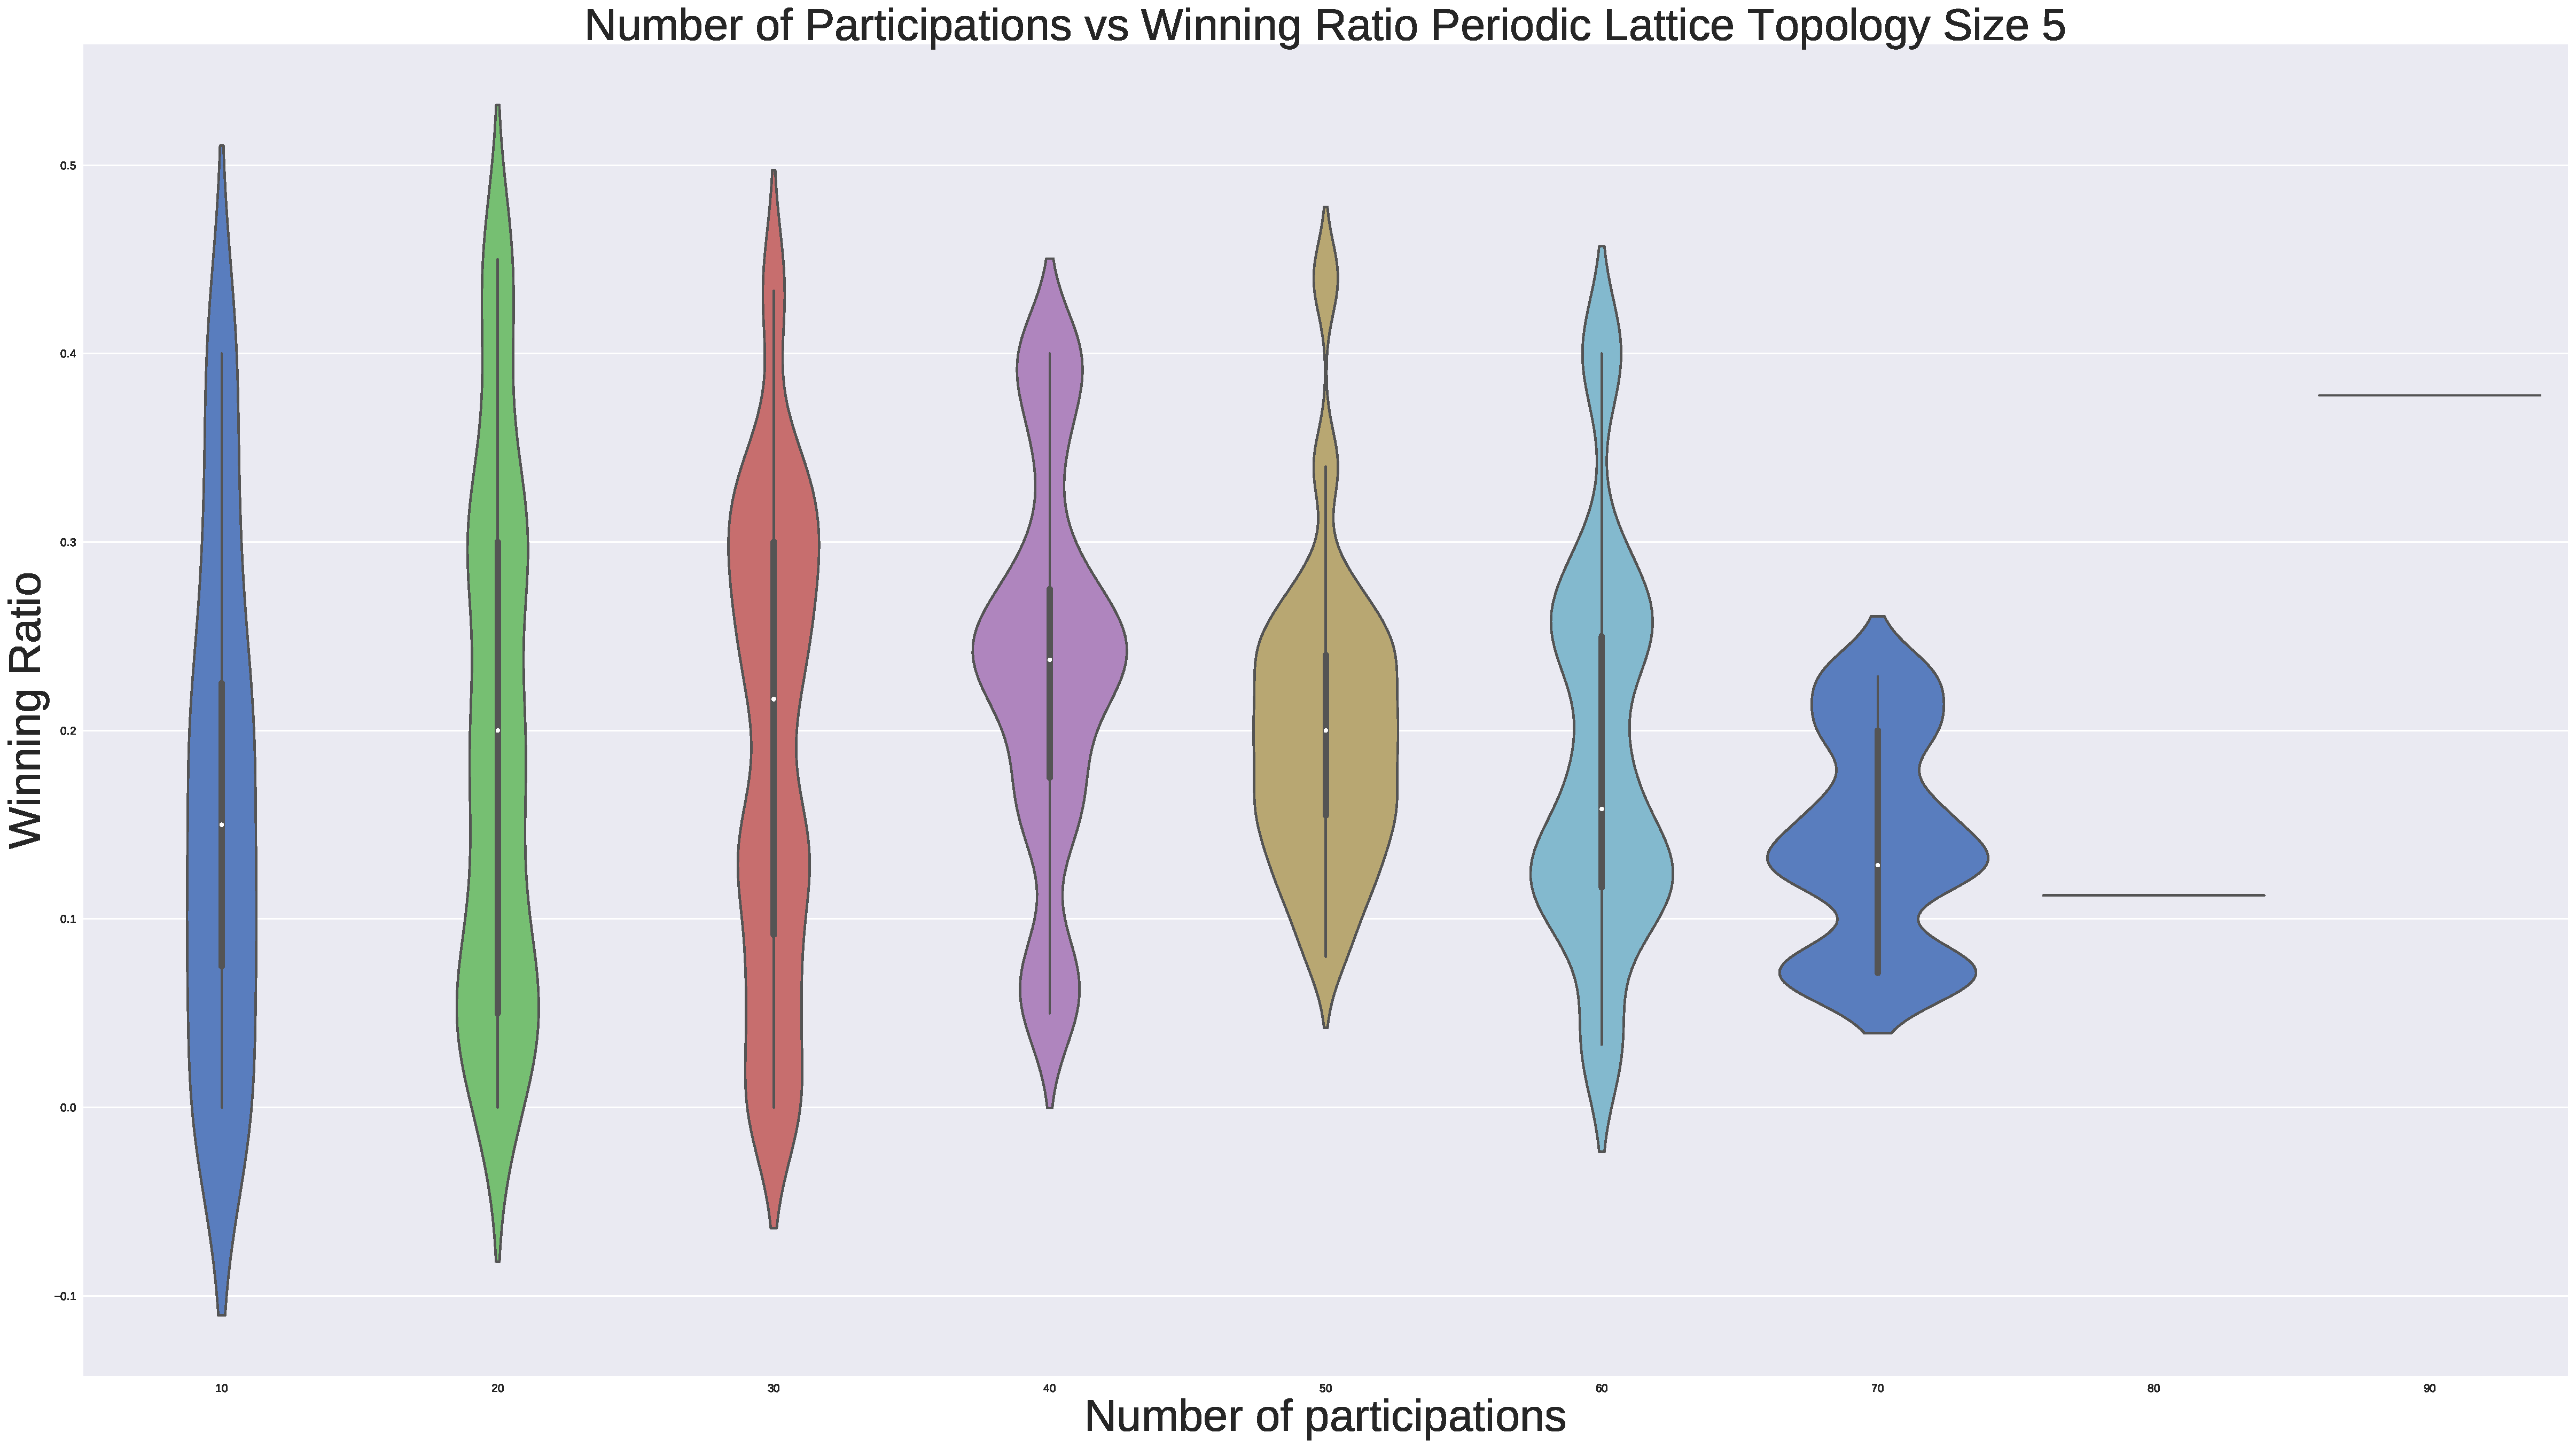
\includegraphics[width=\linewidth]{chapter-three/participation-ratio-violin-Periodic-Lattice-5.pdf}
    \caption{Winning Ratio vs Number of Participations Periodic Lattice Tournament Size 5.}
    \end{subfigure}
\hfill
    \begin{subfigure}[t]{0.75\textwidth}\centering
    \centering
        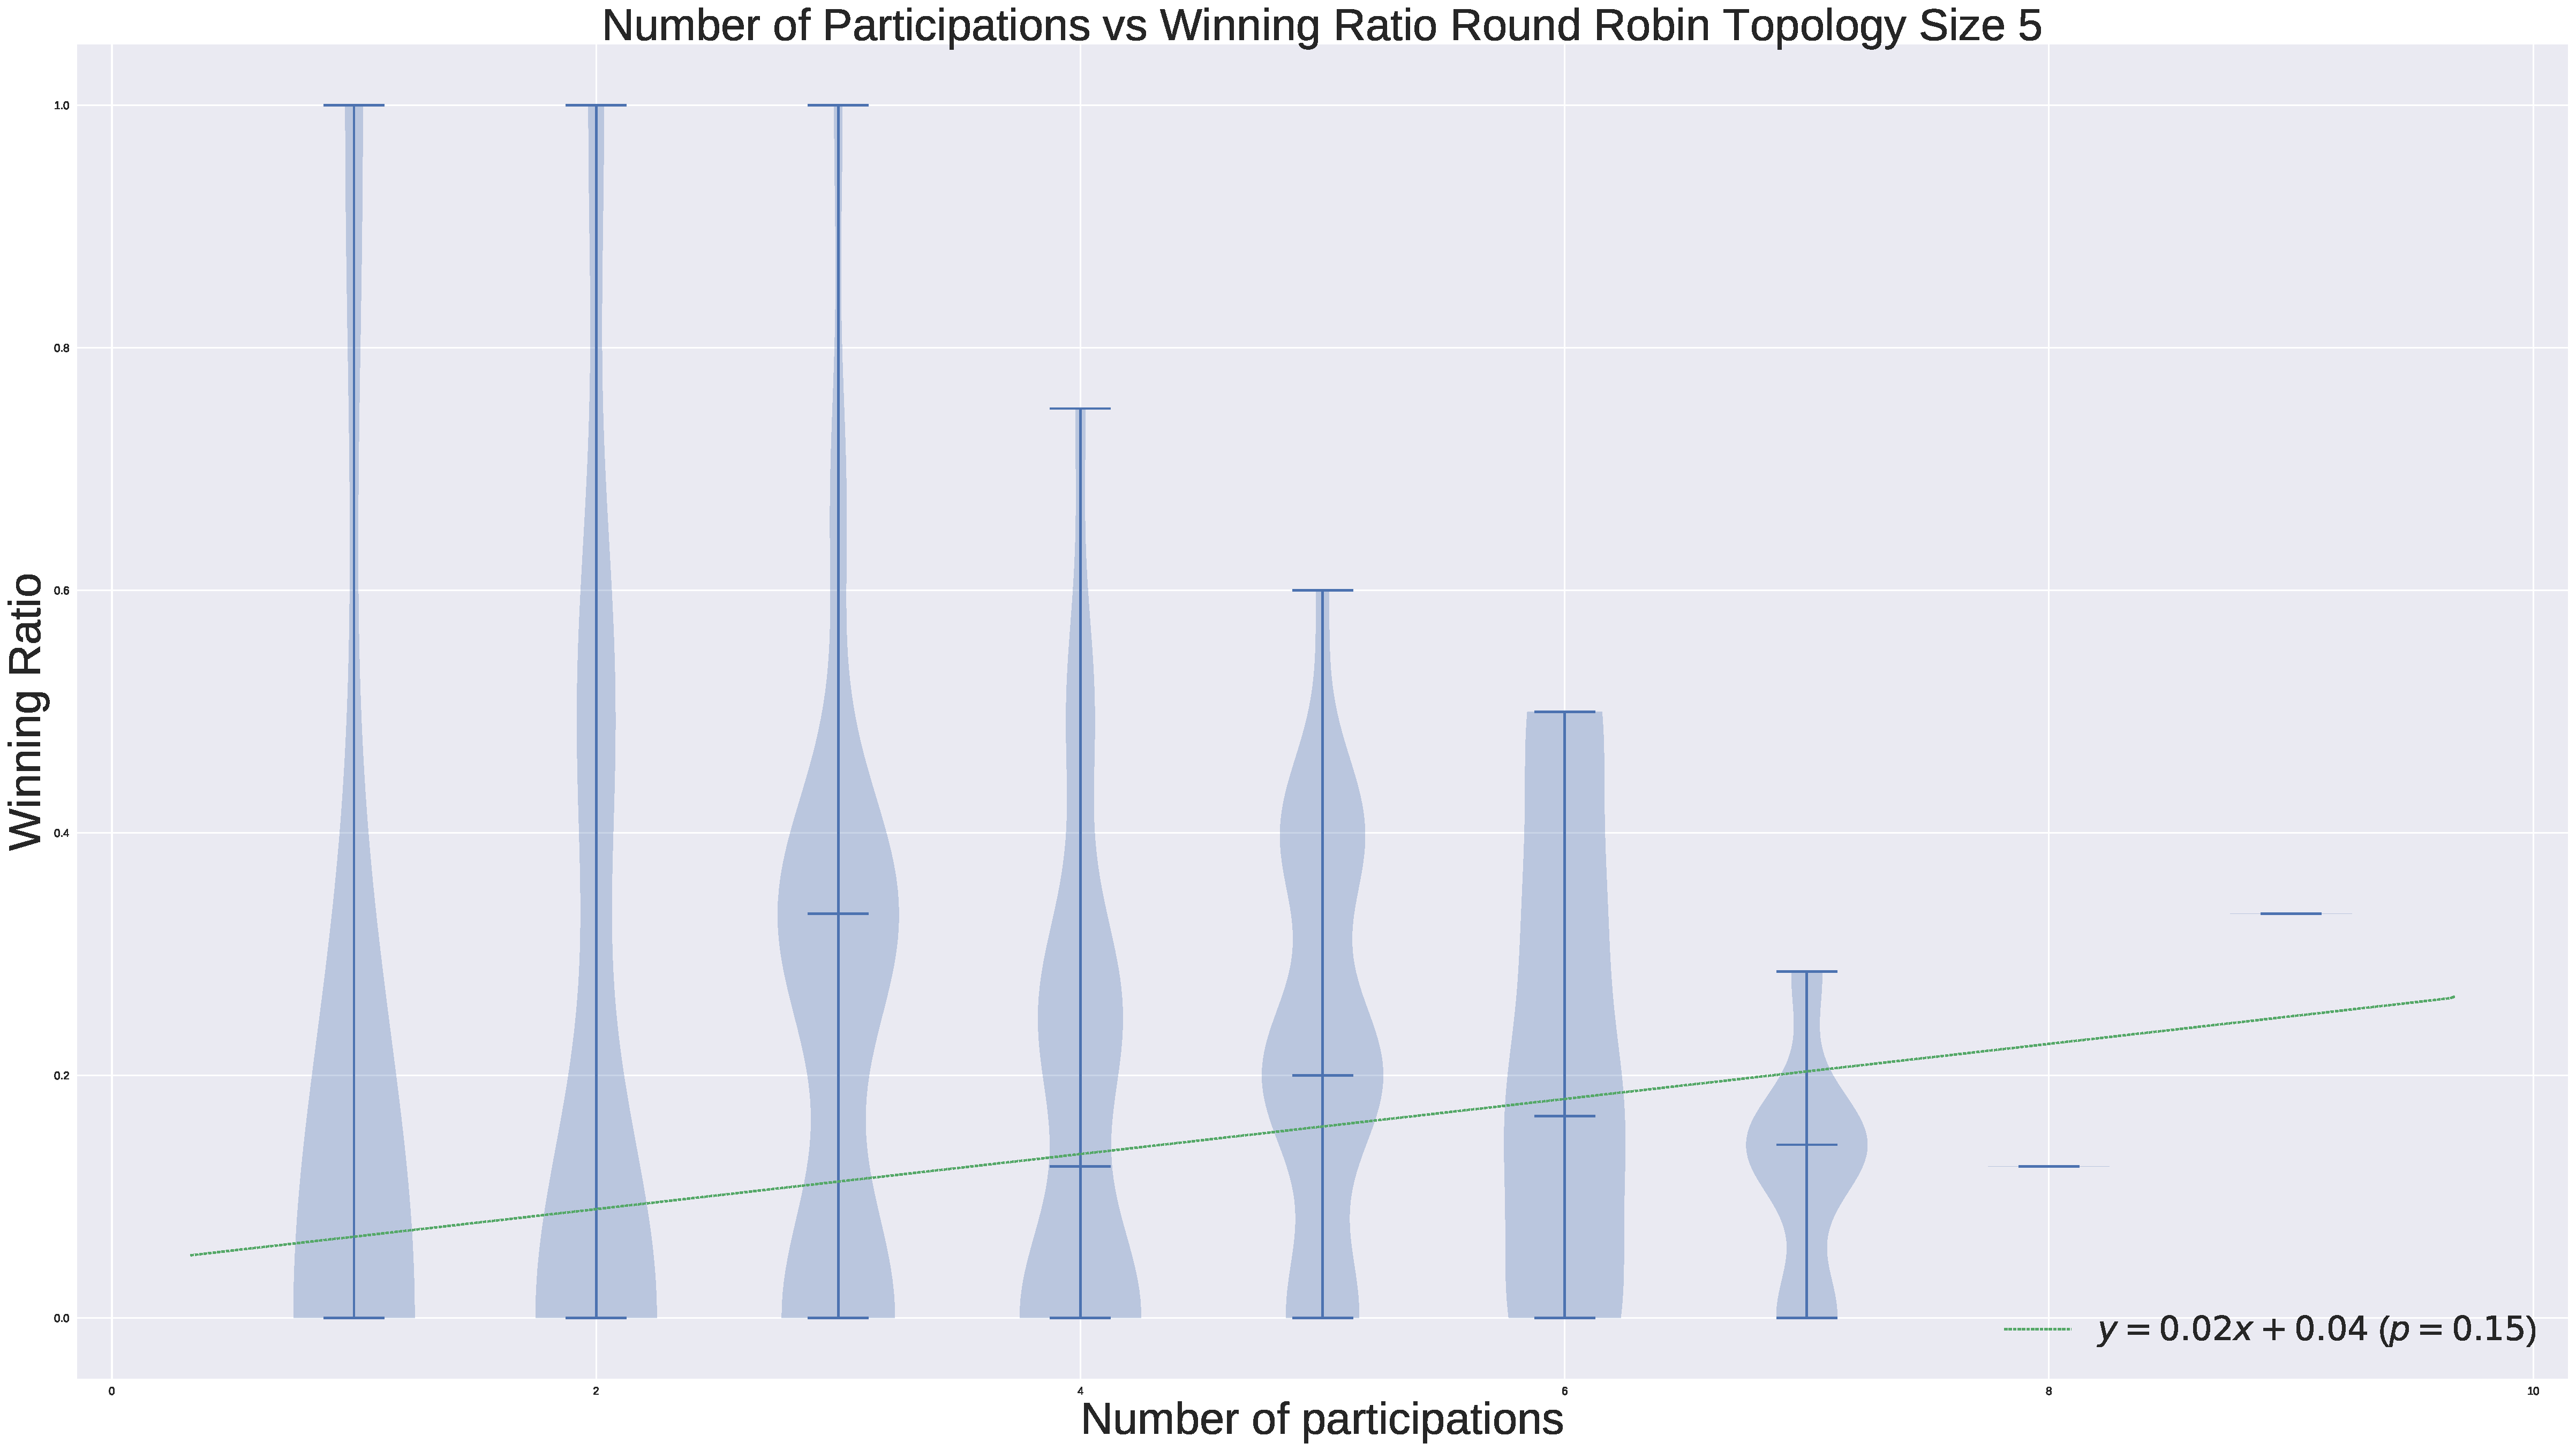
\includegraphics[width=\linewidth]{chapter-three/participation-ratio-violin-Round-Robin-5.pdf}
    \caption{Winning Ratio vs Number of Participations Round Robin Tournament Size 5.}
    \end{subfigure}
\caption{Winning Ratio vs Number of Participations Tournament Size 5.}
\label{fig:winning-ratio-participations-five}
\end{figure}

\begin{figure}[H]
\centering

    \begin{subfigure}[t]{0.75\textwidth}
    \centering
        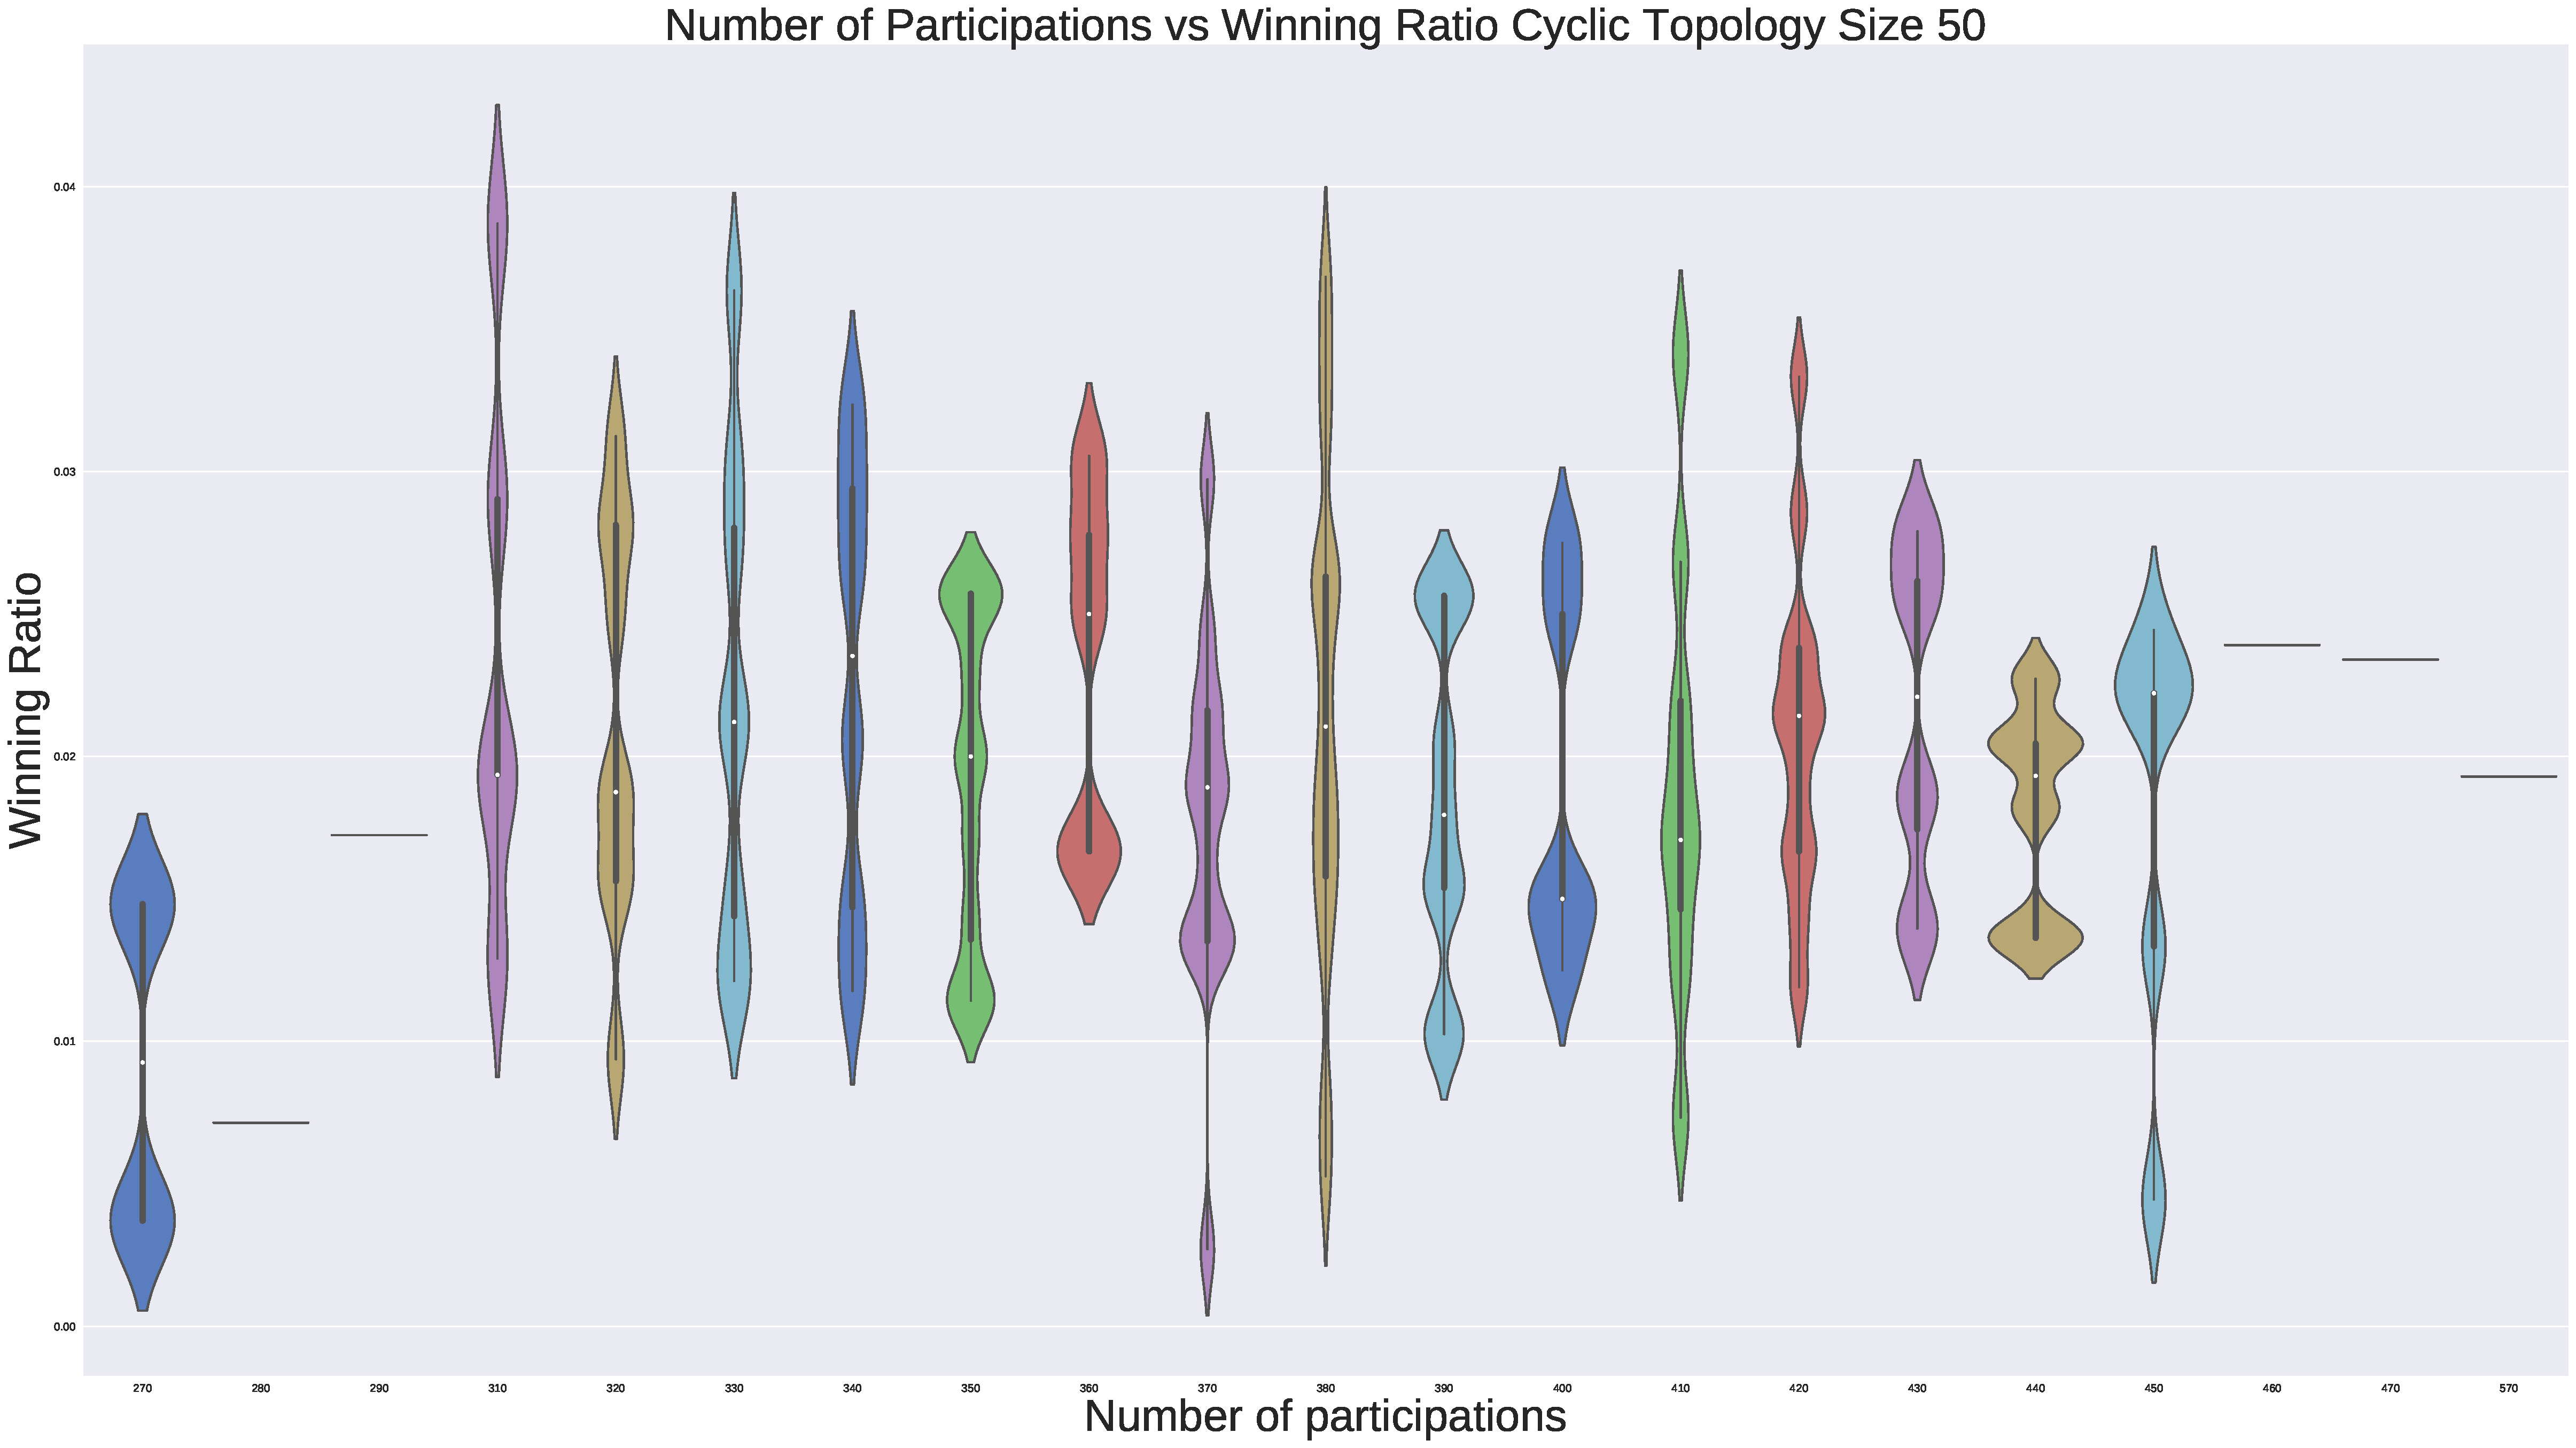
\includegraphics[width=\linewidth]{chapter-three/participation-ratio-violin-Cyclic-50.pdf}
    \caption{Winning Ratio vs Number of Participations Cyclic Tournament Size 50.}
    \end{subfigure}
\hfill
    \begin{subfigure}[t]{0.75\textwidth}\centering
    \centering
        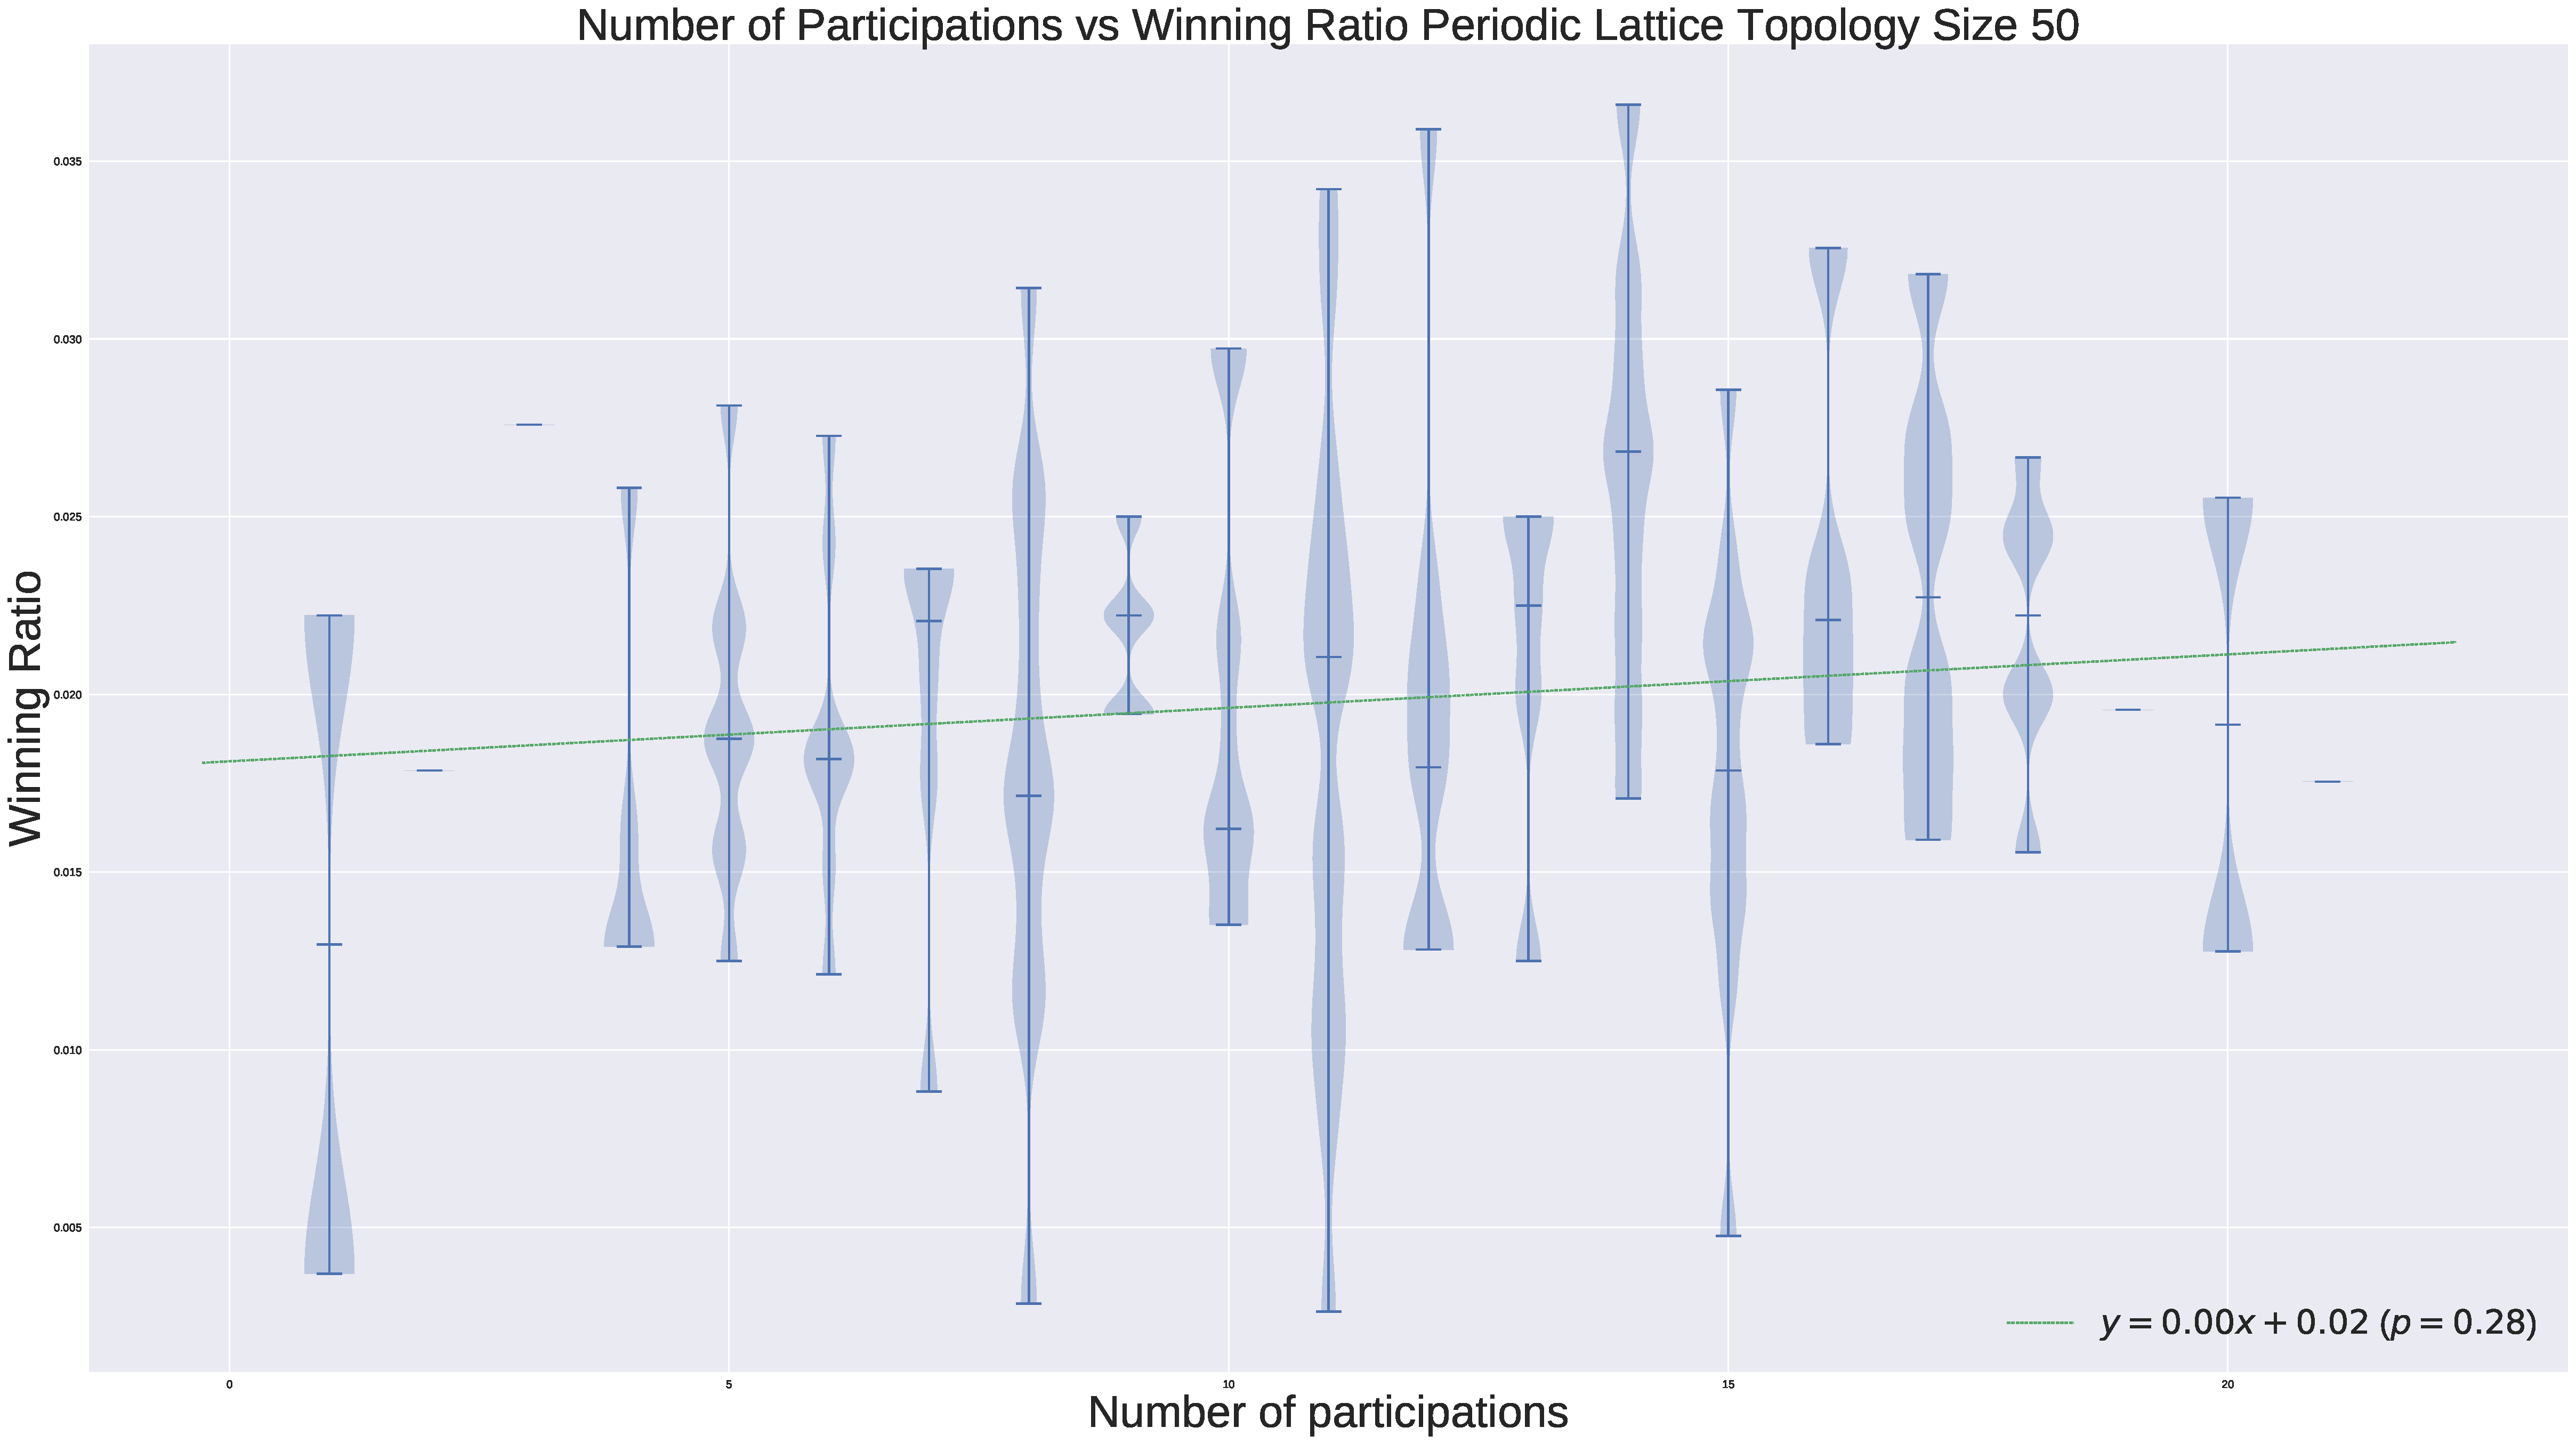
\includegraphics[width=\linewidth]{chapter-three/participation-ratio-violin-Periodic-Lattice-50.pdf}
    \caption{Winning Ratio vs Number of Participations Periodic Lattice Tournament Size 50.}
    \end{subfigure}
\hfill
    \begin{subfigure}[t]{0.75\textwidth}\centering
    \centering
        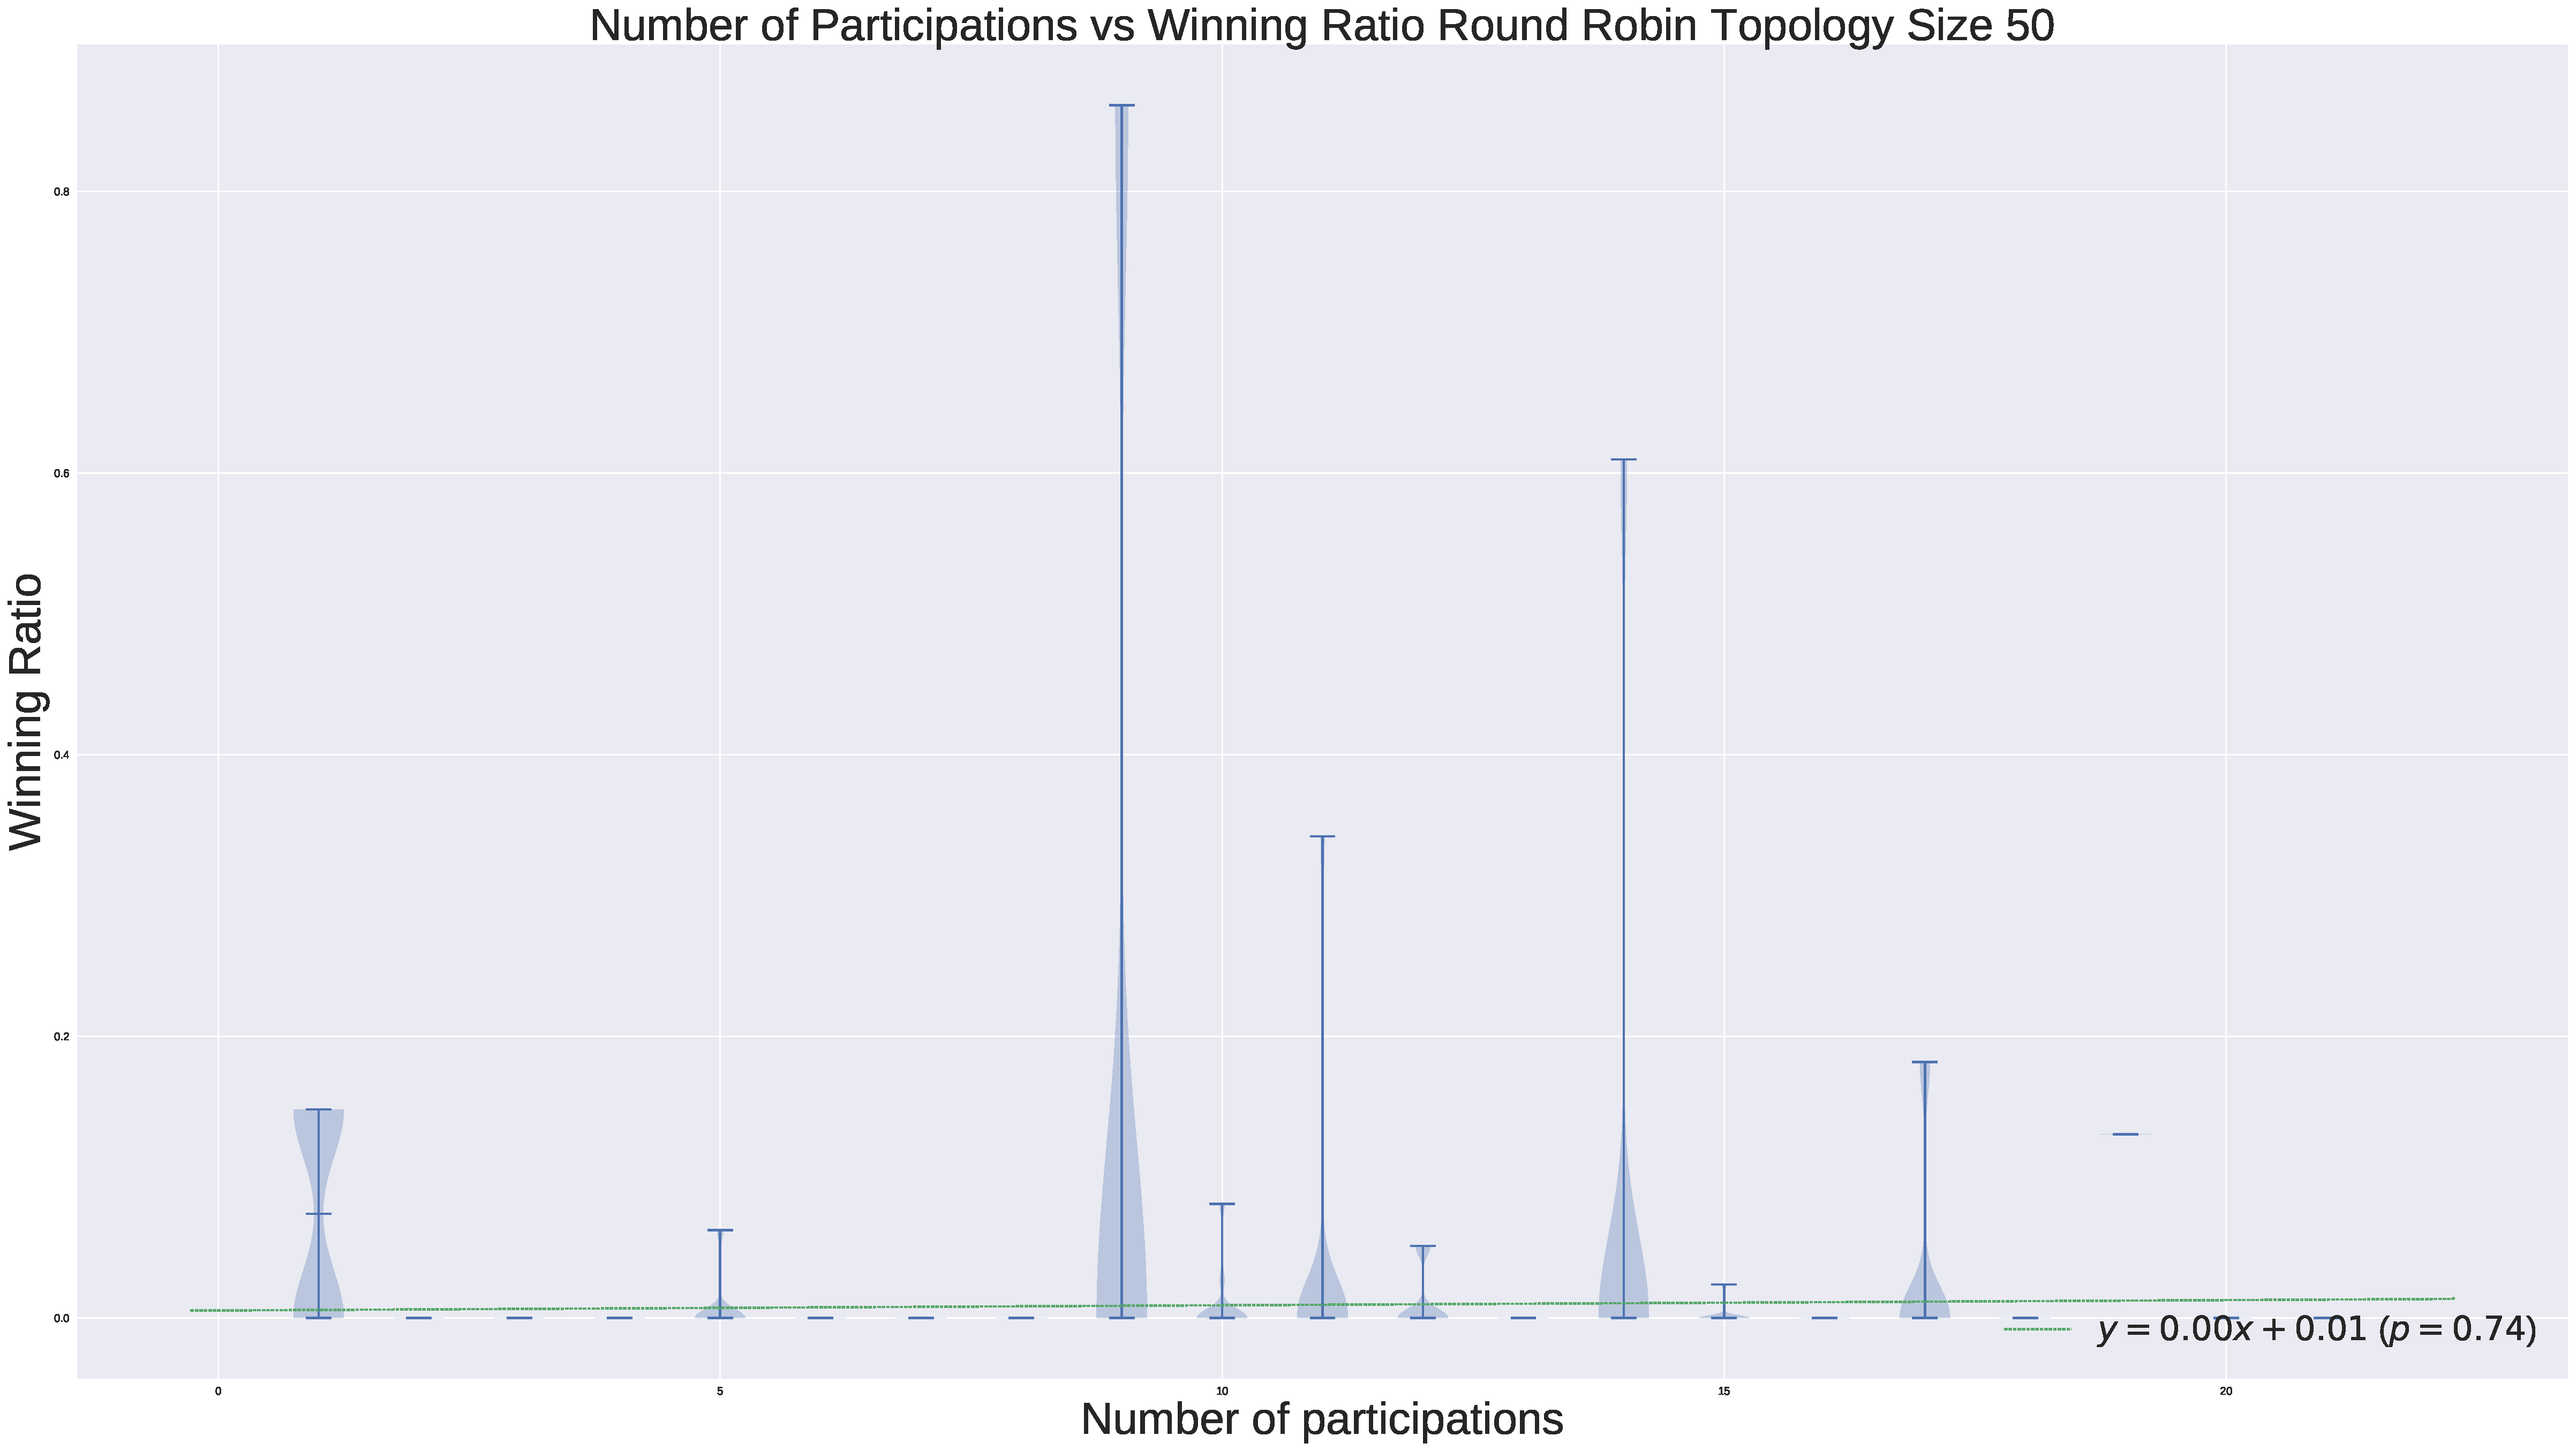
\includegraphics[width=\linewidth]{chapter-three/participation-ratio-violin-Round-Robin-50.pdf}
    \caption{Winning Ratio vs Number of Participations Round Robin Tournament Size 50.}
    \end{subfigure}
\caption{Winning Ratio vs Number of Participations Tournament Size 50.}
\label{fig:winning-ratio-participations-fifty}
\end{figure}

In this subsection the winning ratio has been covered. The strategies were ranked
based on their winning ratio in each of the
six experiments. Line plots that illustrate the devolution in the strategies
rankings, were conducted. Indicating that Raider could be an overall well performed
strategy. Reasons as to why are being investigated. For example the correlation
of the winning ratio and number of participation has been examined. Though
they were not many significant results, connecting winning ratio and participation.
In the next subsection, the Normalized Average Score achieved by the strategies
will be investigated.

\subsection{Normalized Average Scores}
\label{sub:normalized_av_score}

The normalized average score is calculated by dividing the average score per
turn per opponent
of each strategy with their participation counts. Then the average score
is plotted against the strategies. As shown in both
Figures~\ref{fig:average-score-five} and~\ref{fig:average-score-fifty}.

For all six experiments the normalized average score seems to have a lot
of variation. Which indicates each strategy performed differently at given
points of the same experiment. These could be because of the opponent or the
whole neighborhood.

\begin{figure}[H]
\centering
    \begin{subfigure}[t]{0.8\textwidth}
    \centering
        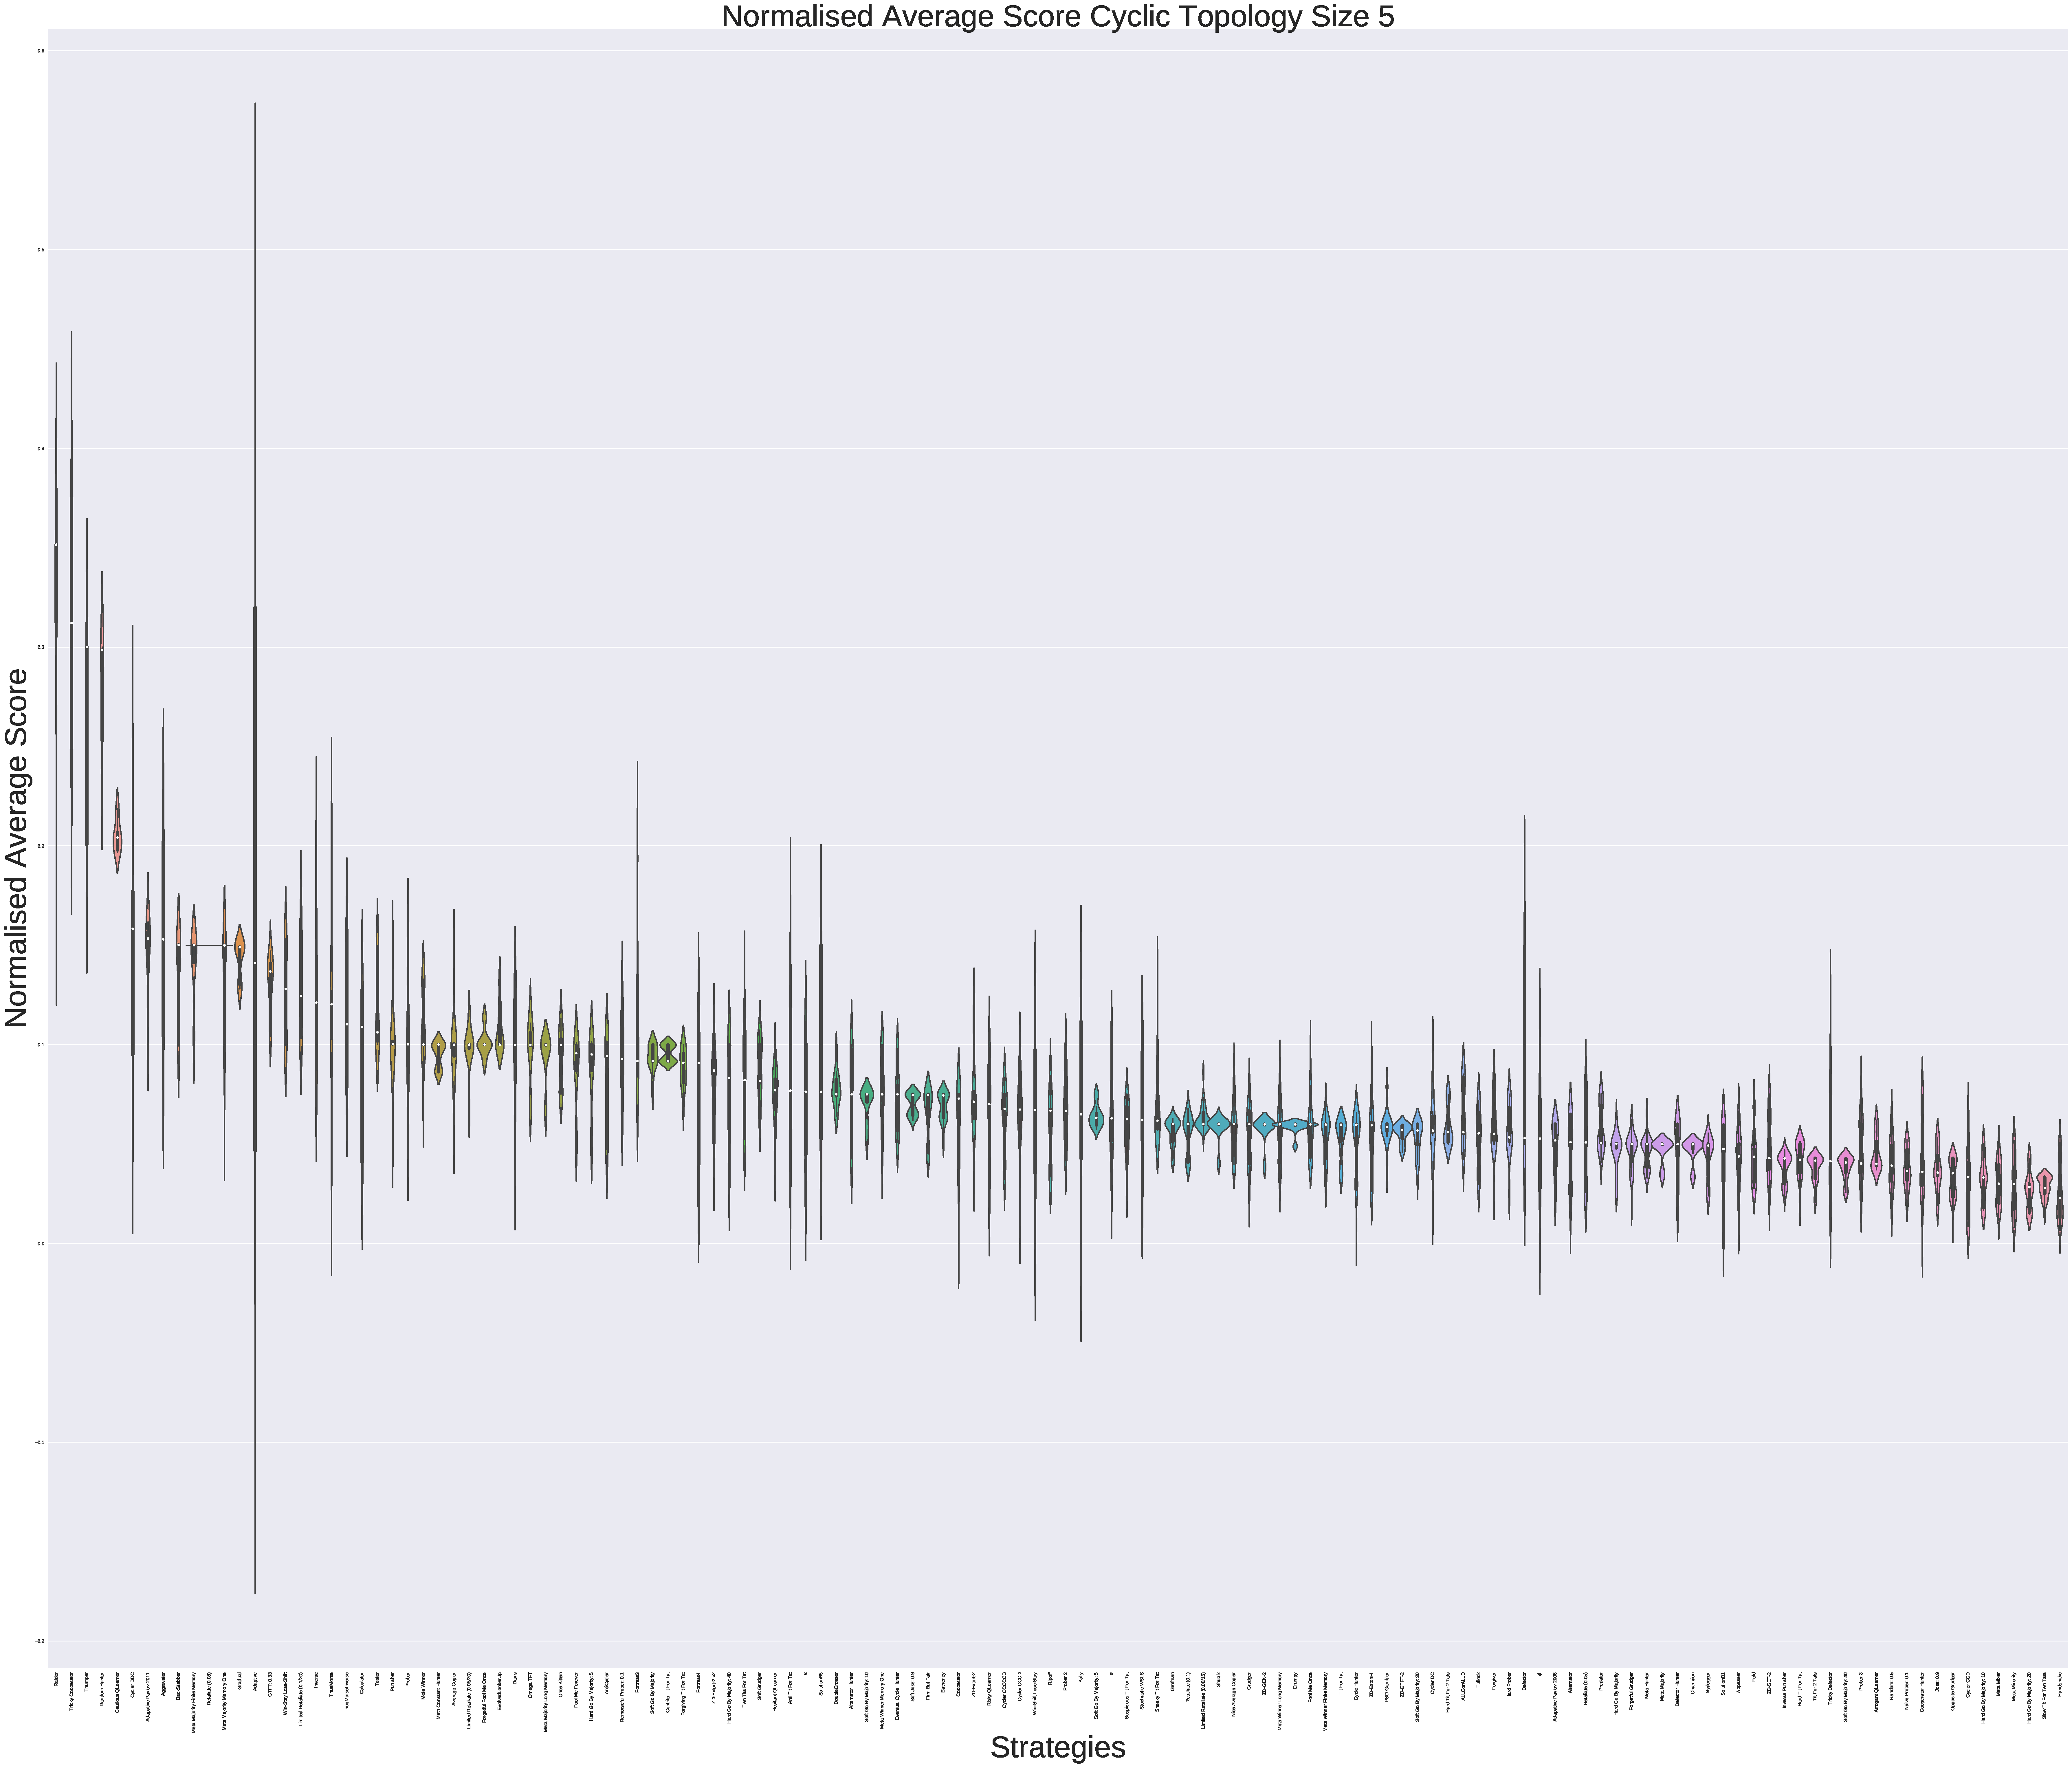
\includegraphics[width=\linewidth]{chapter-three/normalised-score-Cyclic-5.pdf}
    \caption{Normalized Average Score Cyclic Topology Size 5.}
    \end{subfigure}
\hfill
    \begin{subfigure}[t]{0.8\textwidth}\centering
    \centering
        \includegraphics[width=\linewidth]{chapter-three/normalised-score-Periodic-Lattice-5.pdf}
    \caption{Normalized Average Score Periodic Lattice Topology Size 5.}
    \end{subfigure}
\hfill
    \begin{subfigure}[t]{0.8\textwidth}\centering
    \centering
        \includegraphics[width=\linewidth]{chapter-three/normalised-score-Round-Robin-5.pdf}
    \caption{Normalized Average Score Round Robin Topology Size 5.}
    \end{subfigure}
\caption{Normalized Average Score for all Three Topologies Size 5.}
\label{fig:average-score-five}
\end{figure}

\begin{figure}[H]
\centering
    \begin{subfigure}[t]{1\textwidth}
    \centering
        \includegraphics[width=\linewidth]{chapter-three/normalised-score-Cyclic-50.pdf}
    \caption{Normalized average score cycle s=50.}
    \end{subfigure}
\hfill
    \begin{subfigure}[t]{1\textwidth}\centering
    \centering
        \includegraphics[width=\linewidth]{chapter-three/normalised-score-Periodic-Lattice-50.pdf}
    \caption{Normalized average score cycle s=50.}
    \end{subfigure}
\hfill
    \begin{subfigure}[t]{1\textwidth}\centering
    \centering
        \includegraphics[width=\linewidth]{chapter-three/normalised-score-Round-Robin-50.pdf}
    \caption{Normalized Average Score Round Robin Topology Size 50.}
    \end{subfigure}
\caption{Normalized Average Score for all Three Topologies Size 50.}
\label{fig:average-score-fifty}
\end{figure}

Not many conclusions can be made out of this. The high variation could indicate
that the results are completely random. Unfortunately, this could mean that for
any random situation there does not seem to be a strategy that could
achieve a particularly high score although as described in Section~\ref{sub:winning-ratio}
it is possible to ensure a good performance. In the following subsection, a linear
regression model is build for more conclusions.


\subsection{Regression Analysis}
\label{sub:regression}
Finally, a common methodology when investing factors as predictors is building a
regression model. In this subsection two regression models are used to identify
any
factor that can explain the winning ratio and average score of a strategy.
The round robin topology is not included in this subsection analysis as this
investigation aims to understand the effect of network topology.

The first model was built with the winning ratio as the depended variable,
shown here:

\begin{align}
\mathrm{winning.ratio}_{t} = \alpha
    &+ \beta_{1}  \mathrm{degree}_{t} \\
    &+ \beta_{2}  \mathrm{average.neighborhood.score}_{t}    \\
    &+ \beta_{3}  \mathrm{clustering}_{t} \\
    &+ \beta_{4}  \mathrm{number.of.participations}_{t} + \epsilon
\end{align}

\begin{table}[!hbtp]
\centering
\begin{adjustbox}{width=1\textwidth}
\small
\begin{tabular}{@{}|l|l|l|l|l|l|l|l|l|l|l|l|l|@{}}
\toprule
Size & Topology & \multicolumn{2}{l|}{Intercept} & \multicolumn{2}{l|}{degree} & \multicolumn{2}{l|}{average neighborhood score} & \multicolumn{2}{l|}{clustering} & \multicolumn{2}{l|}{participations} & \(R\) - square \\ \midrule
     &          & coef            & p            & coef          & p           & coef                      & p                    & coef             & p              & coef                & p             &          \\ \midrule
size 5  & Cyclic& 0.0344          & 0.00         & 0.0688        & 0.00        & 3.239e-06                 & 0.651                & 0.0              & NA             & 0.0006             & 0.00           & 0.007    \\ \midrule
     & Lattice  & 0.0108          & 0.00         & 0.0431        & 0.00        & 7.447e-06                 & 0.159                 & 0.0108           & 0.00           & -0.0002             & 0.036          & 0.001    \\ \midrule
size 50 & Cyclic& 0.0043          & 0.00         & 0.0087        & 0.00        & -1.386e-06                & 0.00                 & 0                & NA             & -8.156e-07          & 0.216          & 0.002    \\ \midrule
     & Lattice  & 0.0008          & 0.00         & 0.0031        & 0.00        & -4.549e-07                 & 0.00                 & 0.0004           & 0.00           & 2.005e-05          & 0.00          & 0.022    \\ \bottomrule
     neighborhood score affects only the size 50 experiments. In both experiments,
\end{tabular}
\end{adjustbox}
\caption{Regression Results for Winning Ratio Model.}
\label{regression-winning}
\end{table}


For tournaments of size 50, the results it is shown that only the degree seems
to be a stable significant predictor for all three experiments. With a \(p\)
value less that 0.001. Average neighborhood score, has a negative correlation
with the winning ratio. Thus, the
better the neighbors score the less score will a strategy achieve.

Periodic lattice experiments are affected by clustering. Both \(p\) values
are less than 0.05 but are affected with an insignificant amount, less that 0.1.
Participations seems to have a negative effect on the lattice size 5 experiment
but a positive one for the cyclic size 5 and lattice size 50.

Overall, all \(R\) - squaresquare values  are really low. With the highest R- value of a
model being 0.022 for lattice size 50. Thus, the performance of the model can
be characterized as insignificant,

The second model using the normalized average score is the following.

\begin{align}
\mathrm{average.normalised.score}_{t} = \alpha
    &+ \beta_{1}  \mathrm{degree}_{t} \\
    &+ \beta_{2}  \mathrm{average.neighborhood.score}_{t}    \\
    &+ \beta_{3}  \mathrm{clustering}_{t} \\
    &+ \beta_{4}  \mathrm{number.of.participations}_{t} + \epsilon
\end{align}

The model was used to each of the experiments for lattice and cycle topologies
individually. The results of models are shown below, Table~\ref{regression-average} :
% Do you just mean it was used on the total data set? % No, this will go to ch4
\begin{table}[H]
\centering
\begin{adjustbox}{width=1\textwidth}
\small
\begin{tabular}{@{}|l|l|l|l|l|l|l|l|l|l|l|l|l|@{}}
\toprule
Size & Topology & \multicolumn{2}{l|}{Intercept} & \multicolumn{2}{l|}{degree} & \multicolumn{2}{l|}{average neighborhood score} & \multicolumn{2}{l|}{connectivity} & \multicolumn{2}{l|}{participations} & \(R\) - square \\ \midrule
        &          & coef            & p            & coef          & p           & coef                      & p                    & coef             & p              & coef                & p             &          \\ \midrule
size 5  & Cyclic    & 0.028           & 0.00         & 0.0559        & 0.00        & -3.763e-06                & 0.043                & 0.0              & NA             & -0.0016             & 0.00          & 0.457    \\ \midrule
        & Lattice  & 0.0064          & 0.00         & 0.0256        & 0.00        & 1.079e-05                 & 0.00                 & 0.0064           & 0.00           & -0.0016             & 0.00          & 0.549    \\ \midrule
size 50 & Cyclic    & 0.0025          & 0.00         & 0.0051        & 0.00        & -2.168e-07                & 0.00                 & 0                & NA             & -1.602e-05          & 0.00          & 0.120    \\ \midrule
        & Lattice  & 0.0006          & 0.00         & 0.0024        & 0.00        & 1.033e-06                 & 0.00                 & 0.0003           & 0.00           & -1.601e-05          & 0.00          & 0.216    \\ \bottomrule
\end{tabular}
\end{adjustbox}
\caption{Regression Results for Average Score Model.}
\label{regression-average}
\end{table}

In the output, Table~\ref{regression-average}, is shown that degree, average
neighborhood score and participations
are significant predictors for all the experiments with a \(p\) value less than
an 0.0001.
For the cyclic topology, average neighborhood score and participations have negative
coefficient. For example a decrease in participations by one would increase
the average score by 0.0016. Degree on the other hand has a positive coefficient
and connectivity has no effect at all. Furthermore the model for size 5 has
a \(R\) - square value of 0.457, thus it only explains 0.4 variation of the data which is
quite low. For size 50 it is even lower at only 0.12.

Finally, for the lattice topology only participations have a negative coefficient.
Thus the only factor with a reverse influence on average score in the lattice topology.
Connectivity is a significant predictor as well with a coefficient 0.0064 and
0.0003 respectively. Though the \(R\) - square value is still  small,
with a value 0.547 and 0.216 respectively.
Even if there are predictors with a significant \(p\) value, the overall
performance of the model is moderate.

For both models and all set of 6 experiments some predictors can be characterized
as significant. More than one factors have a \(p\) value less than a 0.05, the alpha
that has been set. Even so, the coefficient and the overall R square values are
quite low. Thus, it can not be said that any of this model can predict the
winning ratio neither the average score of a strategy.

\section{Summary}
\label{sub:summary}

A summary of all the analysis previously made, ~\ref{sub:initial_analysis} and
~\ref{sub:analyzing_the_effect_of_the_topologies}, is given in this section.
Moreover, it lists topic for further research to be conducted.

From the analysis that was performed in~\ref{sub:winning-ratio}, the wining ratio
for each strategy for all 6 experiments indicated the following :

\begin{itemize}
  \item For the size 5 experiments, the well performing strategies were Punisher,
        Raider and BackStabber
  \item For the size 50 experiments, the well performing strategies were Nice
        Average Copier, Raider and Fool Me Once
  \item BackStabber, which is one of the highest ranked strategies in the
        Axelrod-Python tournament. Did not win a single tournament in the cyclic
        tournament size 5 experiment
  \item PSO Gambler, the current winner of the Axelrod-Python tournament had the
        highest winning ratio only in the Round Robin 50 experiment
  \item For a Round Robin size 50, most of the strategies finished the experiment
        with winning ratio of zero.
  \item Raider seems to perform highly
\end{itemize}

An attempt to find any significant reason as to why these strategies outperform
the rest gave the findings below:

\begin{itemize}
  \item Winning ratio has a significant difference based on the participations
        number only for the cyclic and lattice topologies of size 5
  \item There is high variation in the average score of each strategy for all
        experiments
  \item Both regression models for the winning ratio and the normalized average
        score did not return any significant results.
\end{itemize}

In conclusion, the strategies winning ratio differs in every topology and
tournament size.
Between the two sizes experiments only Raider seems a repeating strategy in the
high ranked winning ratios. Even so, valid arguments as to how to
successful perform to any given experiment returned zero fundings.

Comparing the results to any other work done in the literature is not possible.
Because this this kind of experiments (which compare a large number of tournaments)
have not been conducted before.
The Axelrod-Python library tournament could be used  a measure of comparison.
Still two (PSO Gambler, BackStabber) of the best overall strategies of that
tournament have only made a brief appearance.

Further actions to the experiments and can be taken for this point on.
Producing a more complete data set for each experiment and carrying out a more
in depth analysis. One could argue that all above experiments
were conducted in simple topologies and a small number of repetitions. Thus, the
next step is to use more complex networks for topologies and conduct a larger
number of tournaments.

\chapter{Complex Networks Experiments}
\label{chap:Four}

\section{Introduction}
In this chapter, an additional experiment on the spatial topology of the IPD
is performed using complex networks. The spatial tournaments will be created using
three different methods. The methods will be explained and the network topologies produced by them
discussed. Followed, by an analysis on the data, including classification methods
based on cooperating ratio, network connectivity and clustering. The cooperating
ratio is a concept provided by the Axelrod-Python library and is computed
by dividing the number of times a strategy cooperated against the number of turns
in a single tournament. Furthermore, regression models are built for the normalized rank.

The issues raised in~\autoref{chap:Three}, will be addessed in the current chapter,
altering various approaches. For example, median ranking is introduced as a more
accurate performance measure and the round robin in treated as a spatial tournament
of a complete topology.

\section{Networks and Methods}
\label{sub:methods}
A complex network is a graph with non-trivial topological features;
features that can not occur in networks such as the ones studied in ~\autoref{chap:Three}.
Such features include, a heavy tail in the degree distribution, a high
clustering coefficient, and hierarchical structure. Complex networks are commonly
used to study computer networks, technological networks and social networks~\cite{VanDerHofstad2009}.

They will also be used in the experiment conducted in this dissertation. Three
different methods, for creating such networks and using them as topologies, have
been used. Each of the methods adopts one of the following models to produce the
required graphs.

\begin{itemize}
	\item Watts-Strogatz, a model for generating graphs with small-world properties\cite{Watts1998}
	\item Erdős–Rényi, a model for generating random graphs~\cite{Erdos1959}
	\item Complete Graph, a graph with the properties of a round robin topology\cite{Harris2010}
\end{itemize}

Each of the models has a different set of parameters and each of the methods
produce different number of networks. The structure of each method is analyzed in
the following subsection.

\subsection{Methods Structure}
\label{sub:experiments-structure}
\subsubsection{Method for small world networks}

In the method of small world networks, the Watts Strogatz model has been used
for generating the required graphs.
The Watts Strogatz model, was proposed by D. Watss and S. Strogatz,
in their work in 1998~\cite{Watts1998}. Their work has been focused on the reproduction
of a network, which interpolated between a regular and a random network.
To achieve this, they considered a random rewiring procedure with the following
rules:

\begin{itemize}
	\item start from a ring lattice with \(n\) vertices and \(k\) the initial edges per vertex
	\item rewire each edges with a probability of \(p\)
\end{itemize}

For the computational approach, \texttt{Networkx}~\cite{networkx} Python library provides the
\texttt{watts\_strogatz\_graph} function. Documentation can be found here:
\url{https://networkx.github.io/documentation/development/reference/generated/networkx.generators.random_graphs.watts_strogatz_graph.html#networkx.generators.random_graphs.watts_strogatz_graph}.
The method's structure is explained
in the Algorithm~\ref{alg:small-world-method}. As shown, the tournament size is
deterministic, ranging for 2 to 50. The initial edges per vertex, ranges from 2
to tournament size minus 1. The random selection of players is repeated 100 times
and each set of selected players is being shuffled for 10 repetitions.

\begin{algorithm}
	\caption{Method for small world networks}\label{alg:small-world-method}
	\begin{algorithmic}
		\Procedure{Small World}{}
		\BState \emph{loop}:
		\For {$\textit{tournament.size} \gets \textit{ 2 to 50}$}
		\For {$\textit{initial.edges.per.vertex} \gets \textit{1 to tournament.size-1}$}
		\For {$\textit{i} \gets \textit{ 0 to 10}$}
		\State $player \gets \textit{random.strategies}$.
		\For {$p \gets \textit{0 to 10}$}
		\State $G \gets \textit{create.watts.strogatz.graph}$.
		\State $edges \gets \textit{G.egdes}$
		\State $results \gets \textit{play.tournament}$.
		\emph{loop}.
		\EndFor
		\EndFor
		\EndFor
		\EndFor
		\EndProcedure
	\end{algorithmic}
\end{algorithm}

\subsubsection{Method for random networks}
In the method of random networks, the desired networks have been produced using the
Erd\"{o}s R\'{e}nyi model.
The model is named after P. Erd\"{o}s and A. R\'{e}nyi, who introduced
the model in 1959~\cite{Erdos1959}. It generates a random graph of \(n\)
vertices and each of the possible edges with probability \(p\).

Similarly, \texttt{Networkx} library provides the function \texttt{binomial\_graph}
for generating such graphs. Documentation can be found here:
\url{https://networkx.github.io/documentation/development/reference/generated/networkx.generators.random_graphs.binomial_graph.html#networkx.generators.random_graphs.binomial_graph}.
Algorithm~\ref{random-method}, illustrate the structure of the method for random
networks. Similarly, the tournament size is not deterministic, instead it
ranges from 2 to 50. A 100 sets of random players are created, and shuffled,
for 10 repetitions.

\begin{algorithm}
	\caption{Method for random networks}\label{random-method}
	\begin{algorithmic}
		\Procedure{Random}{}
		\BState \emph{loop}:
		\For {$\textit{tournament.size} \gets \textit{2 to 50}$}
		\For {$\textit{i} \gets \textit{0 to 100}$}
		\State $player \gets \textit{random.strategies}$.
		\For {$p \gets \textit{0 to 10}$}
		\State $G \gets \textit{create.erdos.renyi.graph}$.
		\State $edges \gets \textit{G.egdes}$
		\State $results \gets \textit{play.tournament}$.
		\emph{loop}.
		\EndFor
		\EndFor
		\EndFor
		\EndProcedure
	\end{algorithmic}
\end{algorithm}

\subsubsection{Method for complete networks}
The method for producing complete networks, uses the \texttt{complete\_graph} function
from the \texttt{Networkx} library:\url{https://networkx.github.io/documentation/development/reference/generated/networkx.generators.classic.complete_graph.html#networkx.generators.classic.complete_graph}
The structure of the method is illustrated by the Algorithm~\ref{complete-method}.

\begin{algorithm}
	\caption{Method for complete networks}\label{complete-method}
	\begin{algorithmic}
		\Procedure{Complete}{}
		\BState \emph{loop}:
		\For {$\textit{tournament.size} \gets \textit{2 to 50}$}
		\For {$\textit{i} \gets \textit{ 0 to 100}$}
		\State $player \gets \textit{random.strategies}$.
		\State $G \gets \textit{create.complete.graph}$.
		\State $edges \gets \textit{G.egdes}$
		\State $results \gets \textit{play.tournament}$.
		\emph{loop}.
		\EndFor
		\EndFor
		\EndProcedure
	\end{algorithmic}
\end{algorithm}

\section{Data generation}
The goal of this chapter is the observation of the strategies behavior when
participating in spatial tournaments of any given topology. Here only three
different types of complex networks will be used. Thus, the data set for this
chapter is a collection of data generated by using the three aforementioned
methods(~\autoref{sub:methods}). Executing these methods requires a high
computational power, considering that over a 1000 of tournaments are
simulated. Thus, they are executed in Raven.

Furthermore, Hierarchical Data Format (HDF5) was used as the file format.
HDF5 is a data model, library, and file format for storing and managing data~\cite{hdf5}.
Python offers an HDF5 binding and HDF5 has various advantages, fitted for the needs
of this chapter. For example, the large amounts of data will be easily stored
and the data can be access without loading them on memory making the analysis
faster.

In ~\autoref{preliminary-analysis}, a preliminary analysis on the individual results of each method
is performed. Followed, by in depth analysis to the whole data set in~\autoref{performance-analysis}.

\section{Preliminary Analysis}
\label{preliminary-analysis}
In this section, the outputs of the three methods are described individually.
Starting with an analysis on the networks attributes that have been produced as topologies,
following a preliminary analysis on the results of their given spatial tournaments.

\subsection{Network Analysis}
\label{sub:network-analysis}
The networks of each method are studied. As introduced in ~\autoref{sub:graph-theory}, the
connectivity and clustering concepts are summarized and reviewed. Due to the
size of experiments and time constraints, not all methods managed to
maximize their tournament sizes, as they have been described in~\autoref{sub:experiments-structure}.

More specifically, for the small world method, a total of 59051 graphs have
been created. The maximum number of nodes achieved is 13. Moreover, the
mean degree, has been 4.75. Thus indicating that
in most tournaments, the average number of neighbors per strategy was 4.
The maximum degree is equal to 12. Further,
the mean connectivity of the small world network is 3.40, the minimum is 0 and the maximum 9.
The clustering coefficient ranges from 0 to 1, with a mean of 0.48. A mean
of 0.48, for the clustering coefficients, indicates that strategies have a
neutral trend towards creating cliques (complete graphs).

\begin{table}[!hbtp]
	\centering
	\begin{adjustbox}{width=0.5\textwidth}
		\small
		\begin{tabular}{cccccccccc}
				\toprule
			\multicolumn{5}{|c|}{Small world Networks Summary Table}           \\ \hline
			     & connectivity & clustering & degree & nodes                  \\ \hline
			mean & 3.40         & 0.48       & 4.75   & 10.00                  \\ \hline
			std  & 2.37         & 0.33       & 2.65   & \multicolumn{1}{c}{-} \\ \hline
			min  & 0.00         & 0.00       & 1.00   & 3.00                   \\ \hline
			max  & 9.00         & 1.00       & 12.00  & 13.00                   \\ \bottomrule
		\end{tabular}
	\end{adjustbox}
	\caption{Small world summary table}
	\label{table:small-world-summary-table}
\end{table}

Illustrating 59051 graphs for understanding the networks of the experiment, is
an impossible task. For this reason, the summary Table~\ref{table:small-world-summary-table}
has been used. Furthermore, eight networks have been randomly selected and
displayer in Figure~\ref{fig:small_networks_illustration}. Mainly to get an idea
of the look of the networks in this method.

\begin{figure}[!hbtp]
	\centering
	\begin{subfigure}[t]{0.30\textwidth}
		\centering
		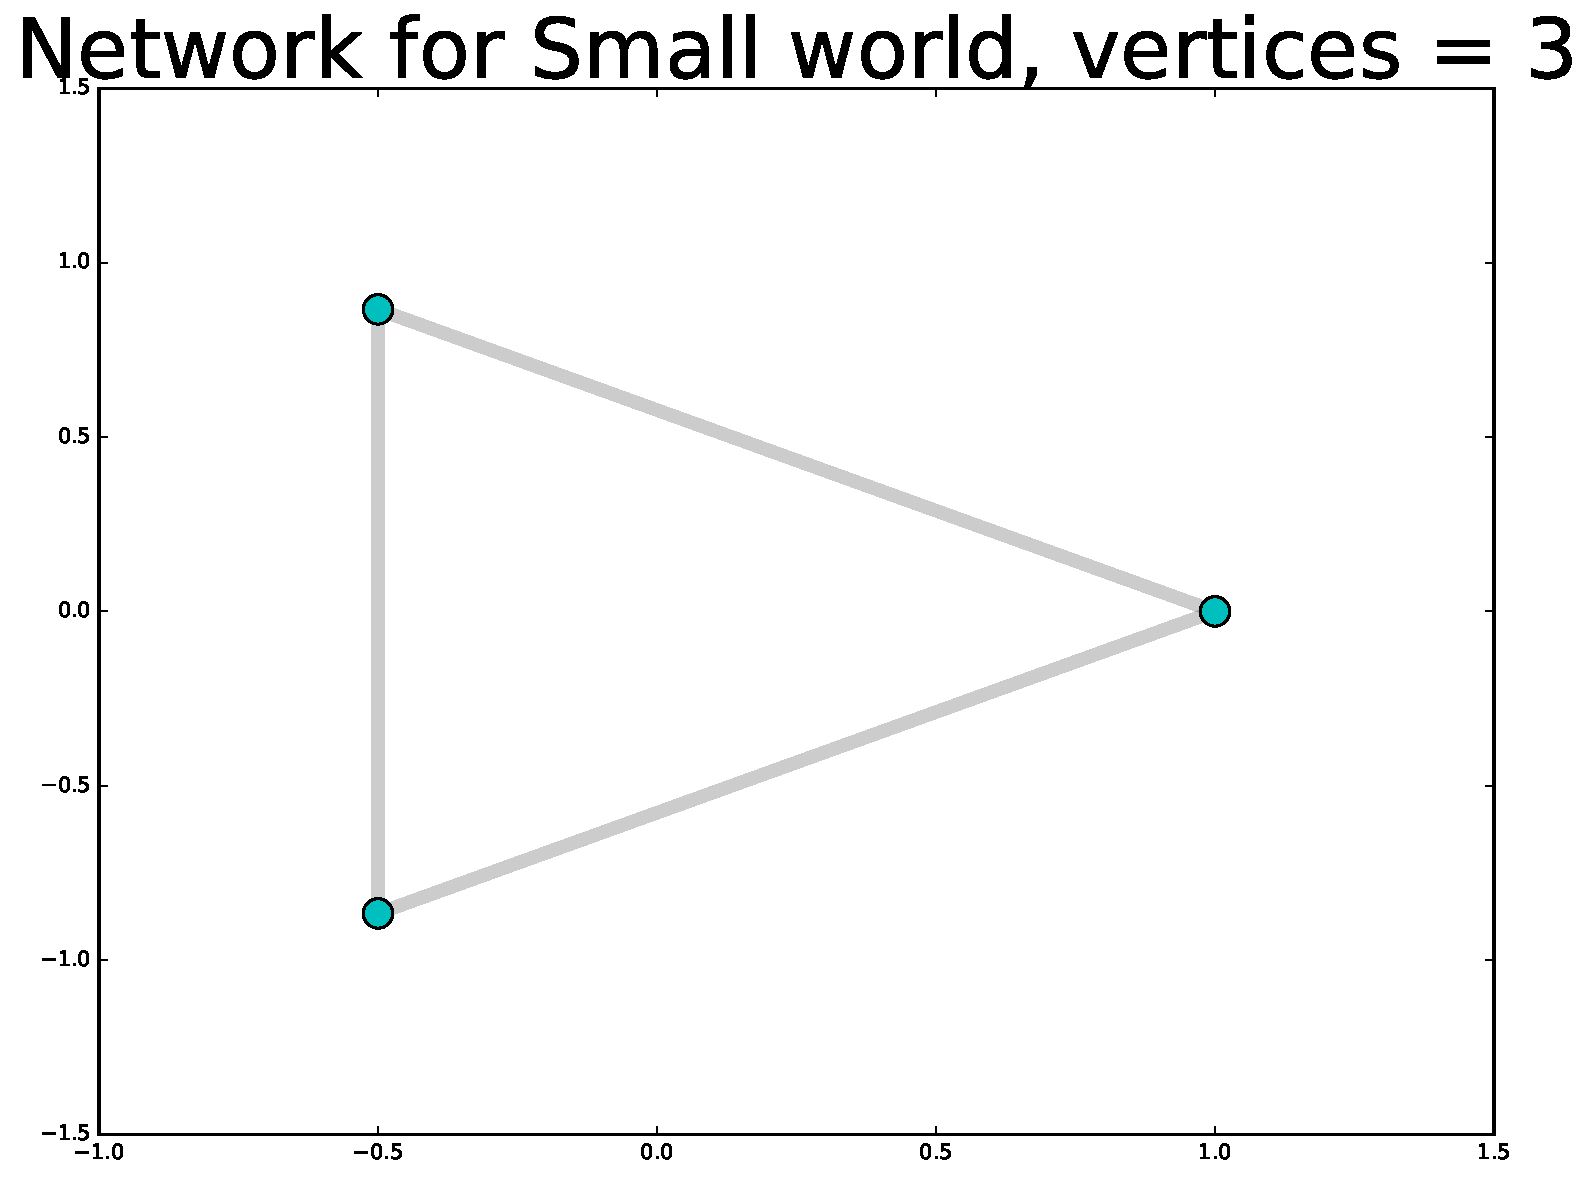
\includegraphics[width=\linewidth]{chapter-four/small__networks_3.pdf}
		\caption{Three nodes}
	\end{subfigure}
	\hfill
	\begin{subfigure}[t]{0.30\textwidth}\centering
		\centering
		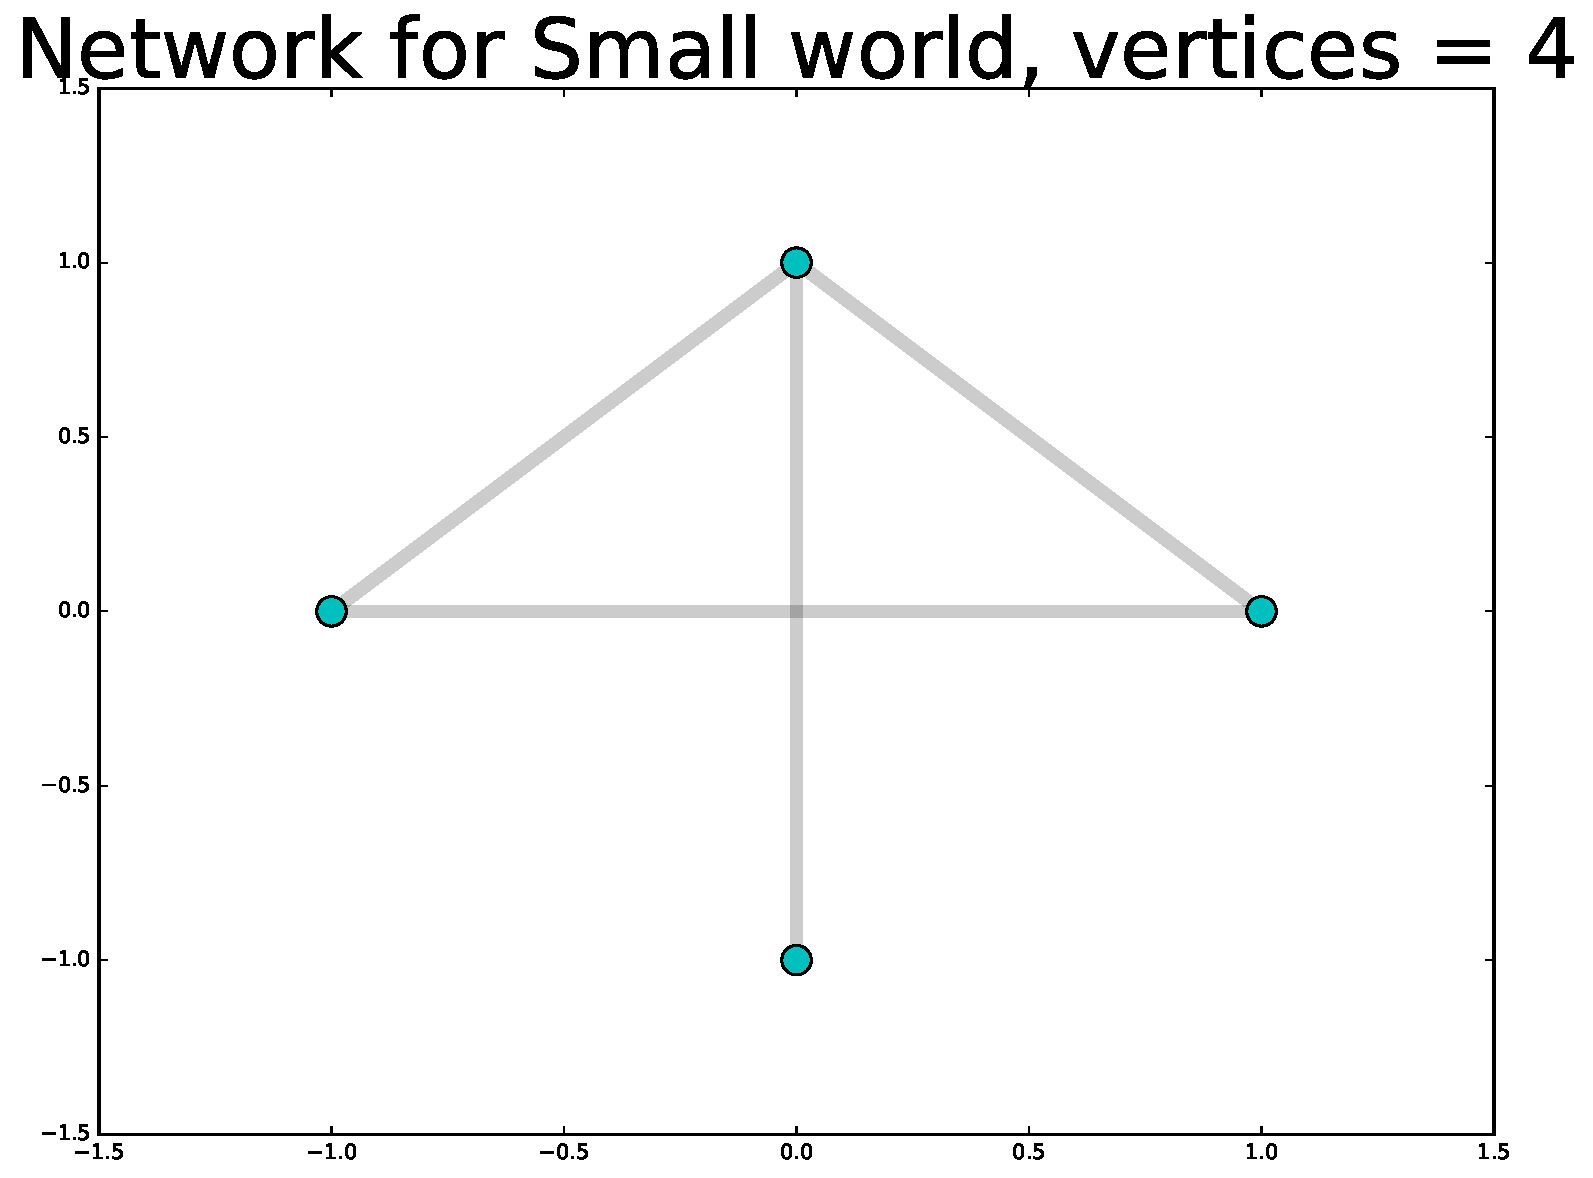
\includegraphics[width=\linewidth]{chapter-four/small__networks_4.pdf}
		\caption{Four nodes}
	\end{subfigure}
	\hfill
	\begin{subfigure}[t]{0.30\textwidth}\centering
		\centering
		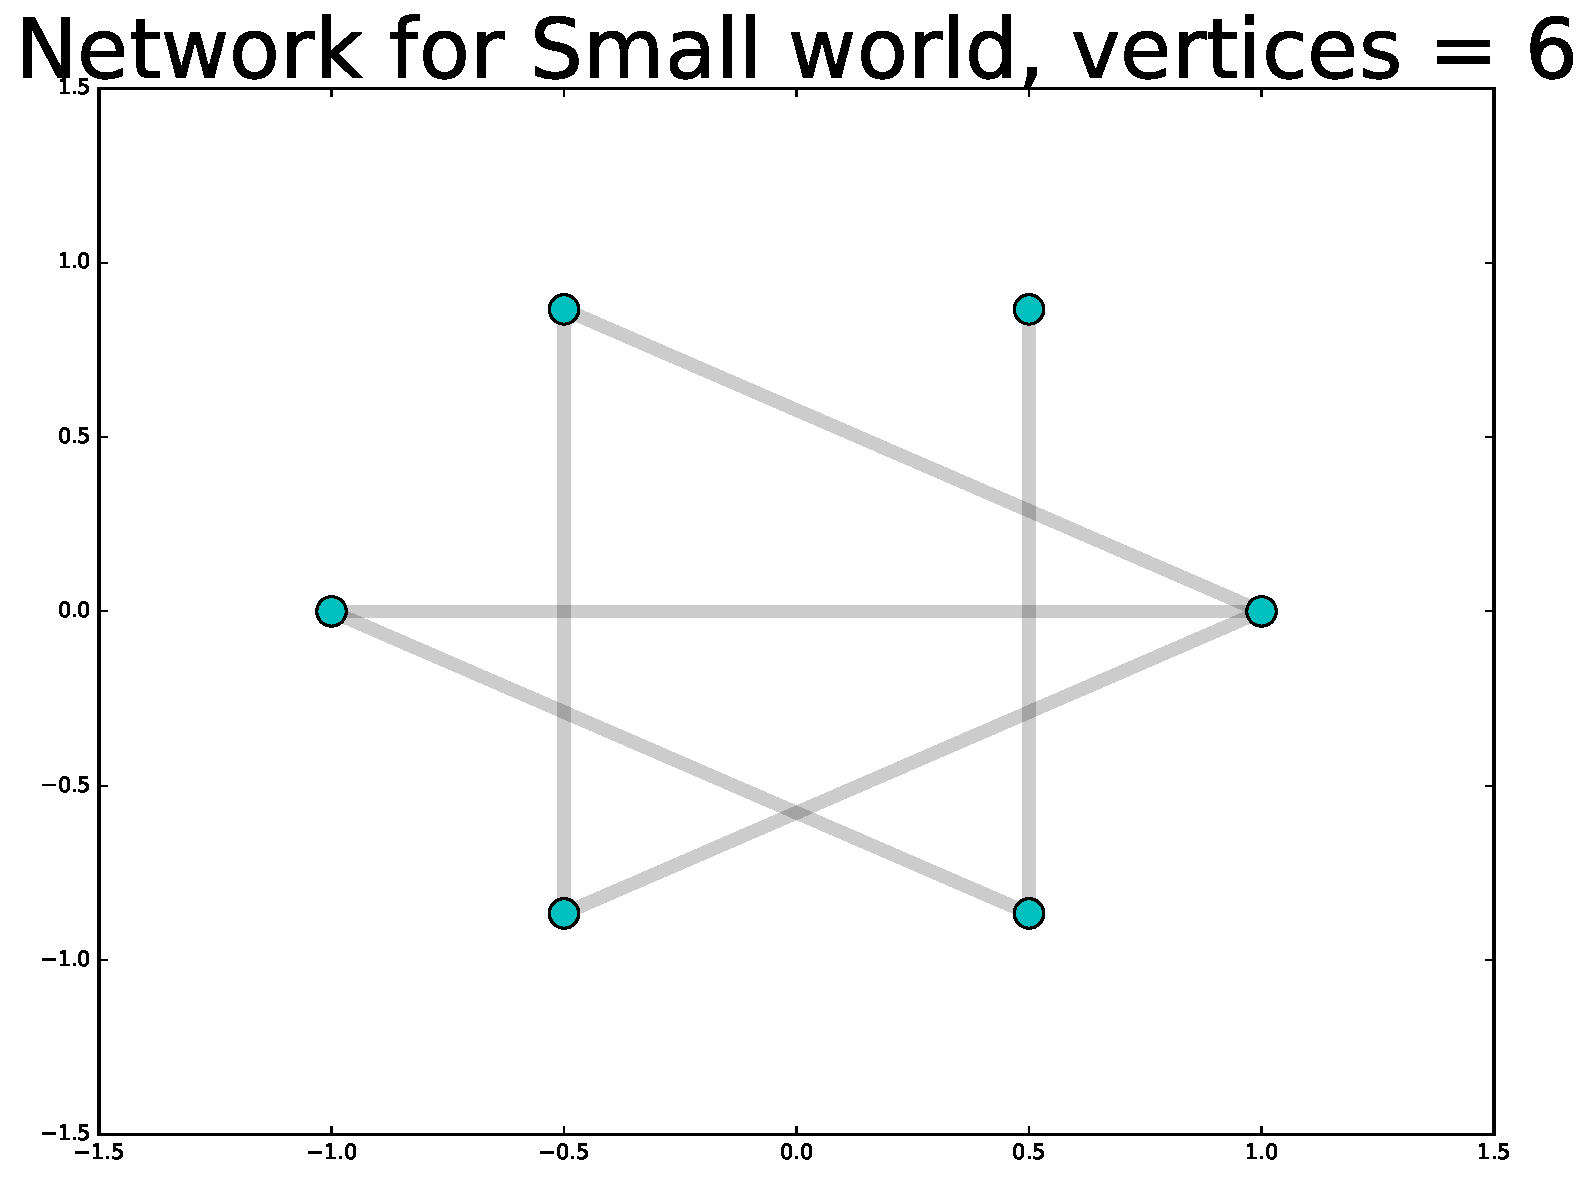
\includegraphics[width=\linewidth]{chapter-four/small__networks_6.pdf}
		\caption{Six nodes}
	\end{subfigure}
	\hfill
	\begin{subfigure}[t]{0.30\textwidth}\centering
		\centering
		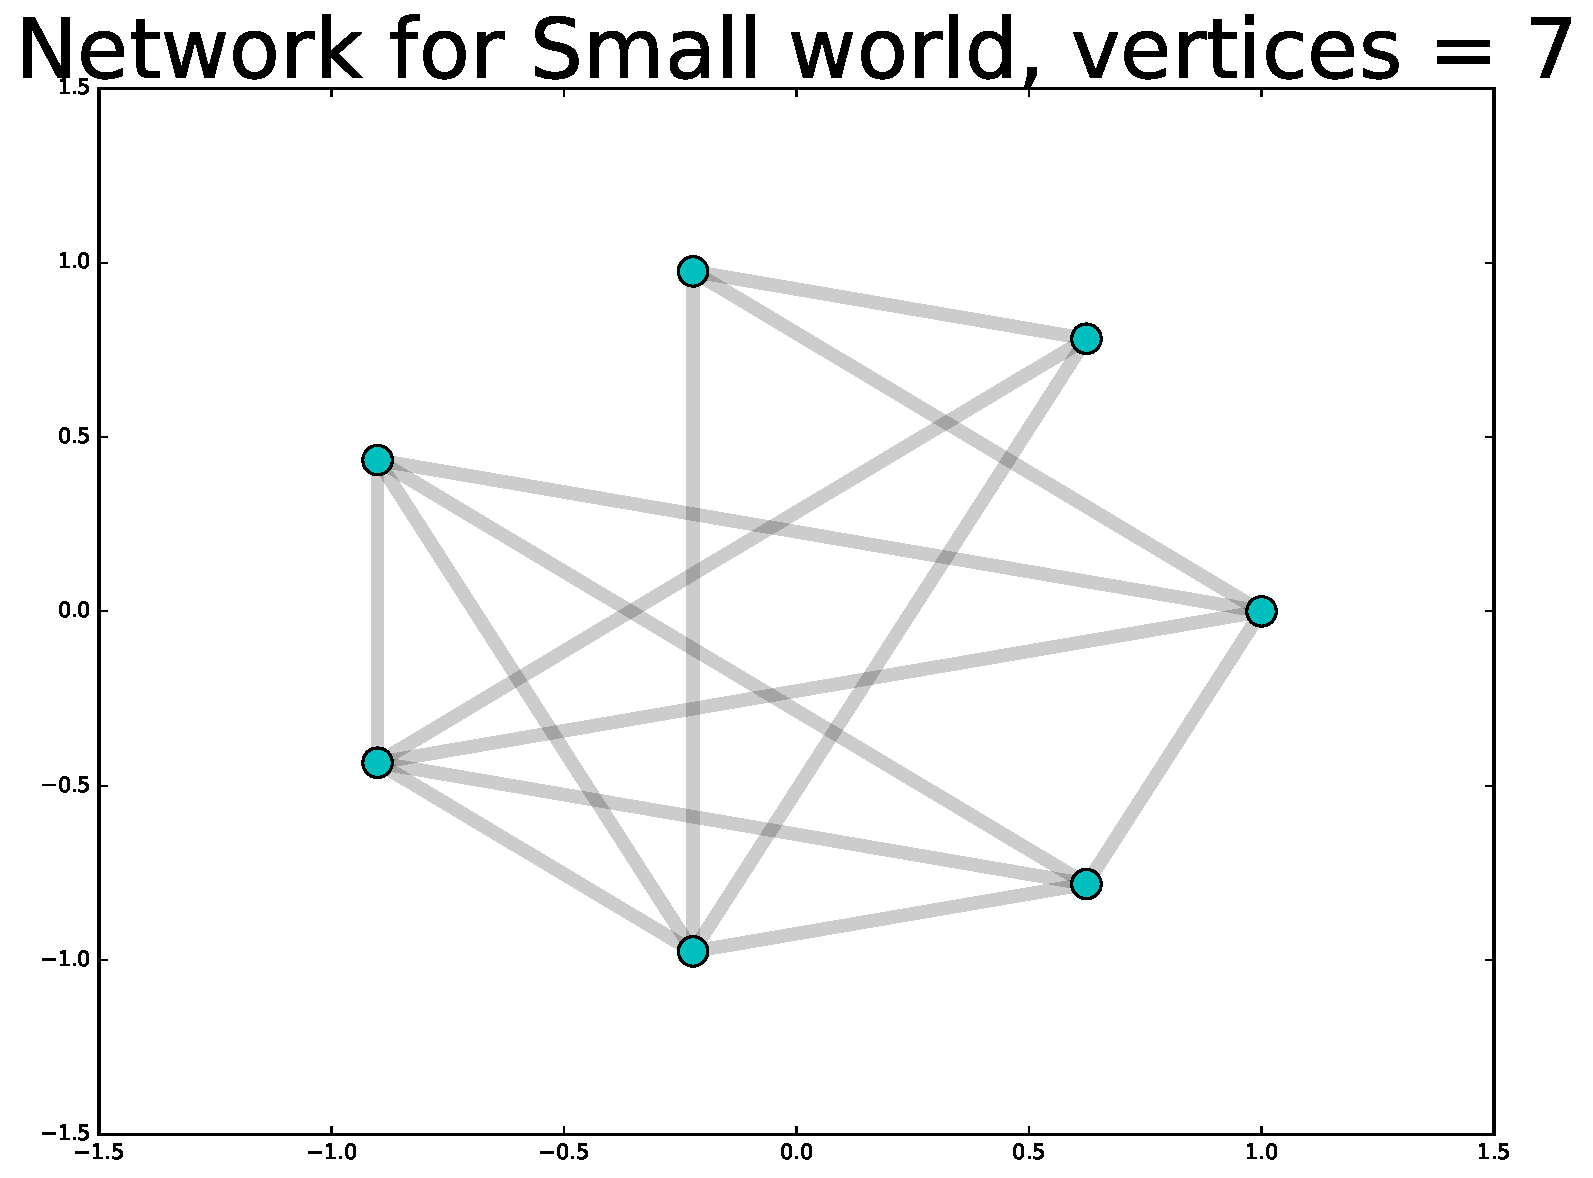
\includegraphics[width=\linewidth]{chapter-four/small__networks_7.pdf}
		\caption{Seven nodes}
	\end{subfigure}
	\hfill
	\begin{subfigure}[t]{0.30\textwidth}\centering
		\centering
		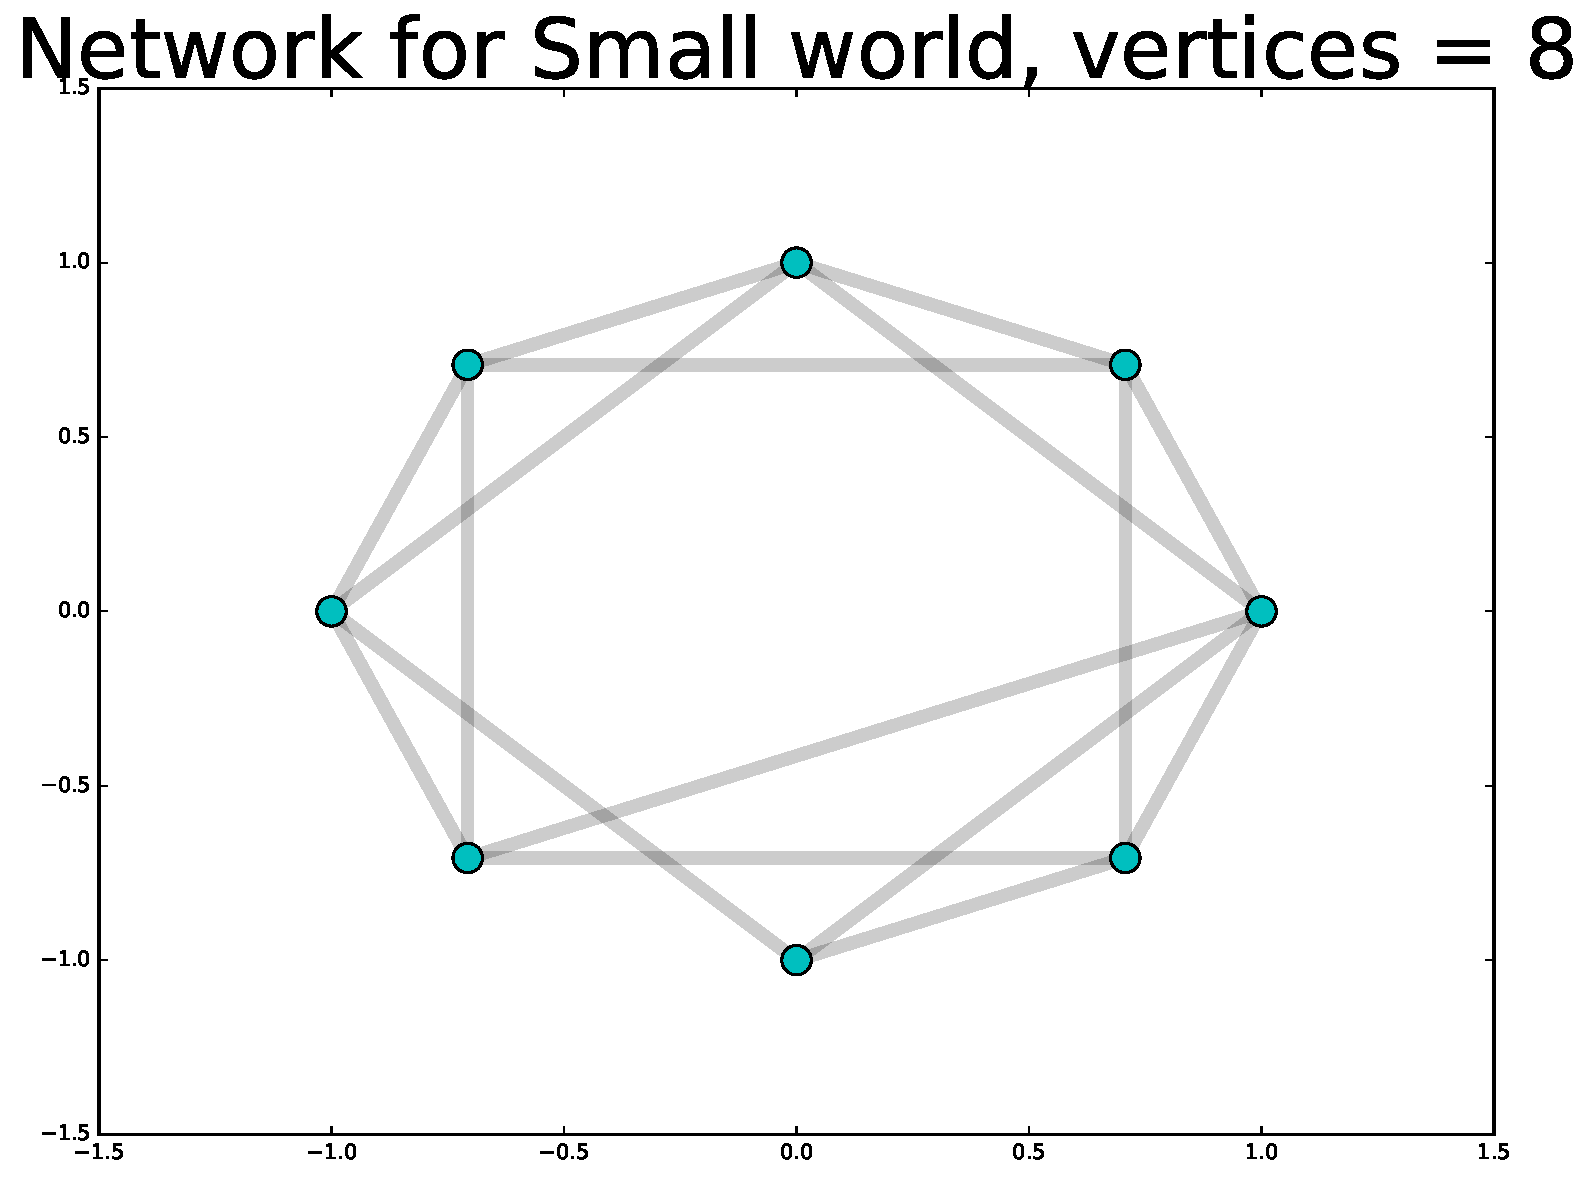
\includegraphics[width=\linewidth]{chapter-four/small__networks_8.pdf}
		\caption{Eight nodes}
	\end{subfigure}
	\hfill
	\begin{subfigure}[t]{0.30\textwidth}\centering
		\centering
		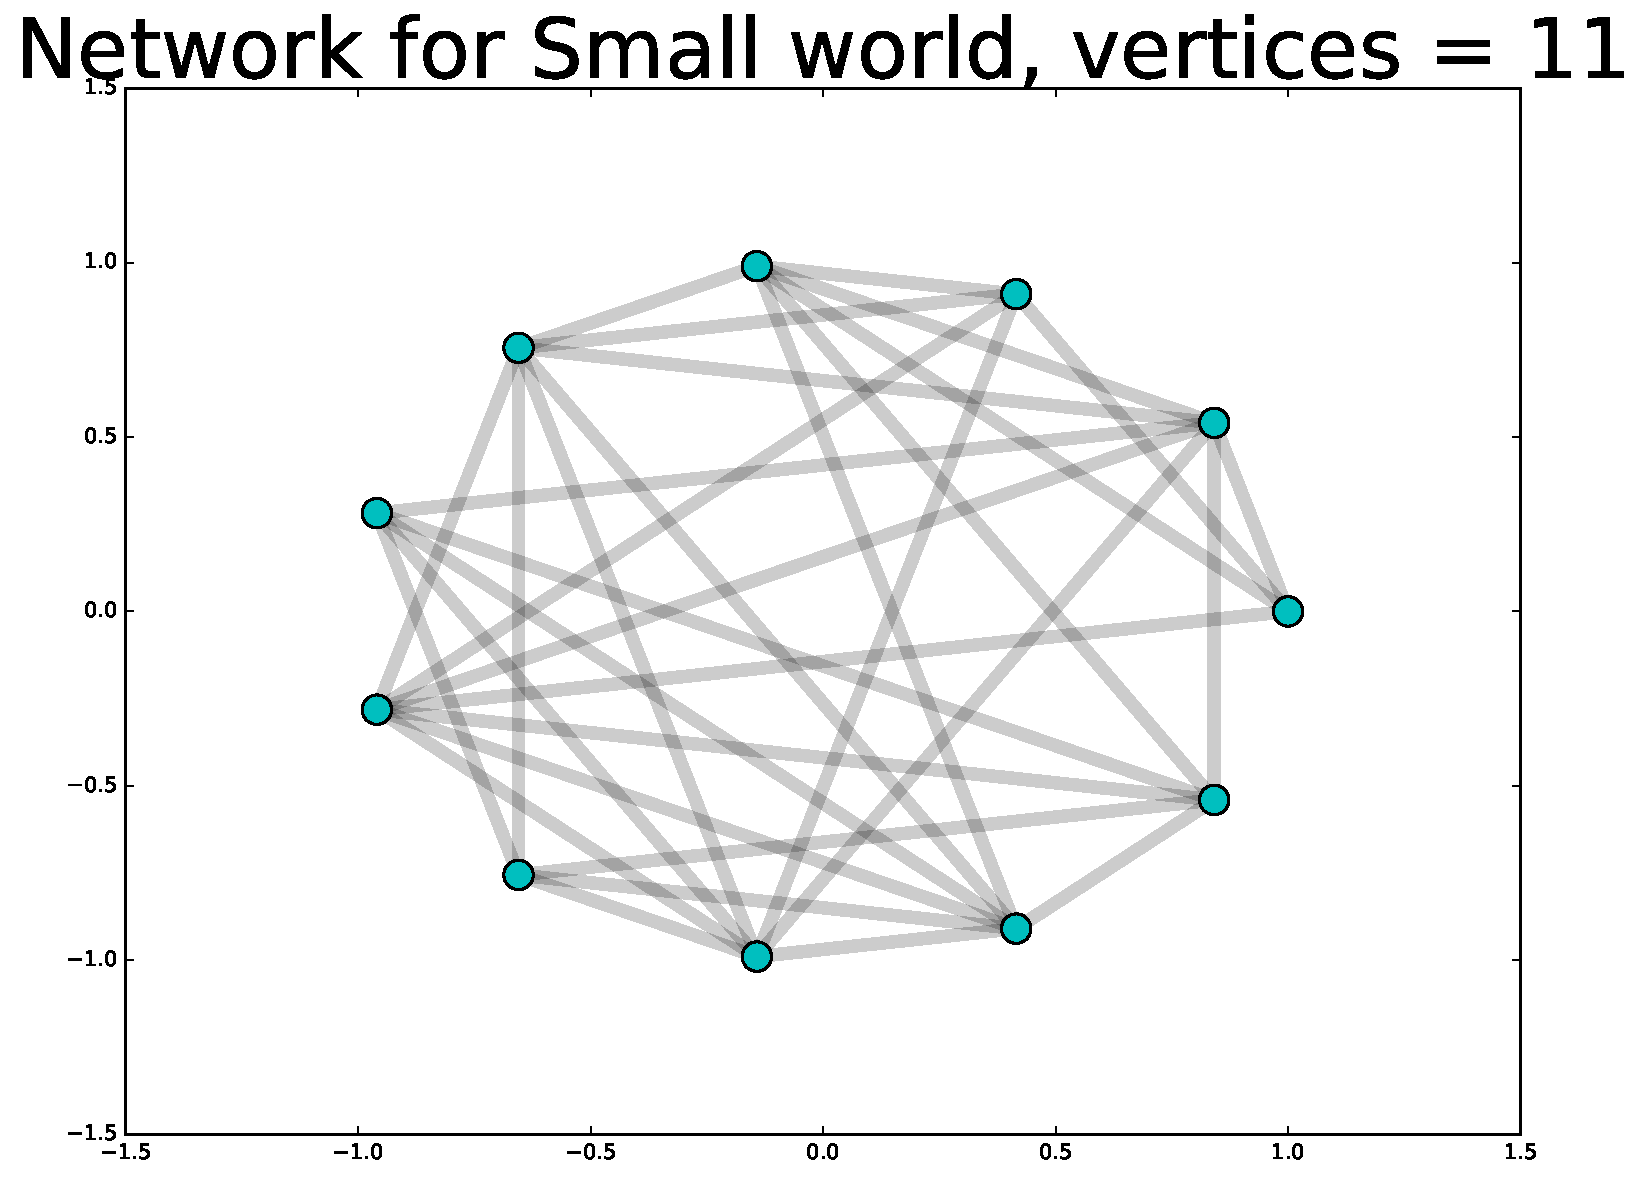
\includegraphics[width=\linewidth]{chapter-four/small__networks_11.pdf}
		\caption{Eleven nodes}
	\end{subfigure}
	\caption{Various Watss Strogatz networks}
	\label{fig:small_networks_illustration}
\end{figure}

Likewise for the random networks method. The experiment did not manage to
achieve the maximum tournament size that had been set. Instead, 21924 have been
created. As shown in Table~\ref{table:binomial-summary-table}, the mean number
of nodes of the experiments has been 20, the minimum 2 and the maximum 29. The
mean connectivity, of a random network, is approximately 8.26, the minimum
0.00 and maximum 28.00.

\begin{table}[!hbtp]
	\centering
	\begin{adjustbox}{width=0.5\textwidth}
		\small
		\begin{tabular}{cccccccccc}
				\toprule
			\multicolumn{5}{|c|}{Random Networks Summary Table}                       \\ \hline
			     & connectivity & clustering & degree & nodes                  \\ \hline
			mean & 8.26         & 0.60       & 11.22  & 19.80                  \\ \hline
			std  & 6.46         & 0.30       & 6.50   & \multicolumn{1}{c}{-} \\ \hline
			min  & 0.00         & 0.00       & 1.00   & 2.00                   \\ \hline
			max  & 28.00        & 1.00       & 28.00  & 29.00                  \\ \bottomrule
		\end{tabular}
	\end{adjustbox}
	\caption{Random summary table}
	\label{table:binomial-summary-table}
\end{table}

The clustering coefficient, of the random networks has a mean value of 0.60. The
mean node number is equal to 20 with a mean degree 11. Thus, in most of the
tournaments that occurred, the strategy had to compete with 11 of it's neighbors.
Once again, six random have been picked and are illustrated in Figure ~\ref{random_networks_illustration}.

\begin{figure}[H]
	\centering
	\begin{subfigure}[t]{0.30\textwidth}
		\centering
		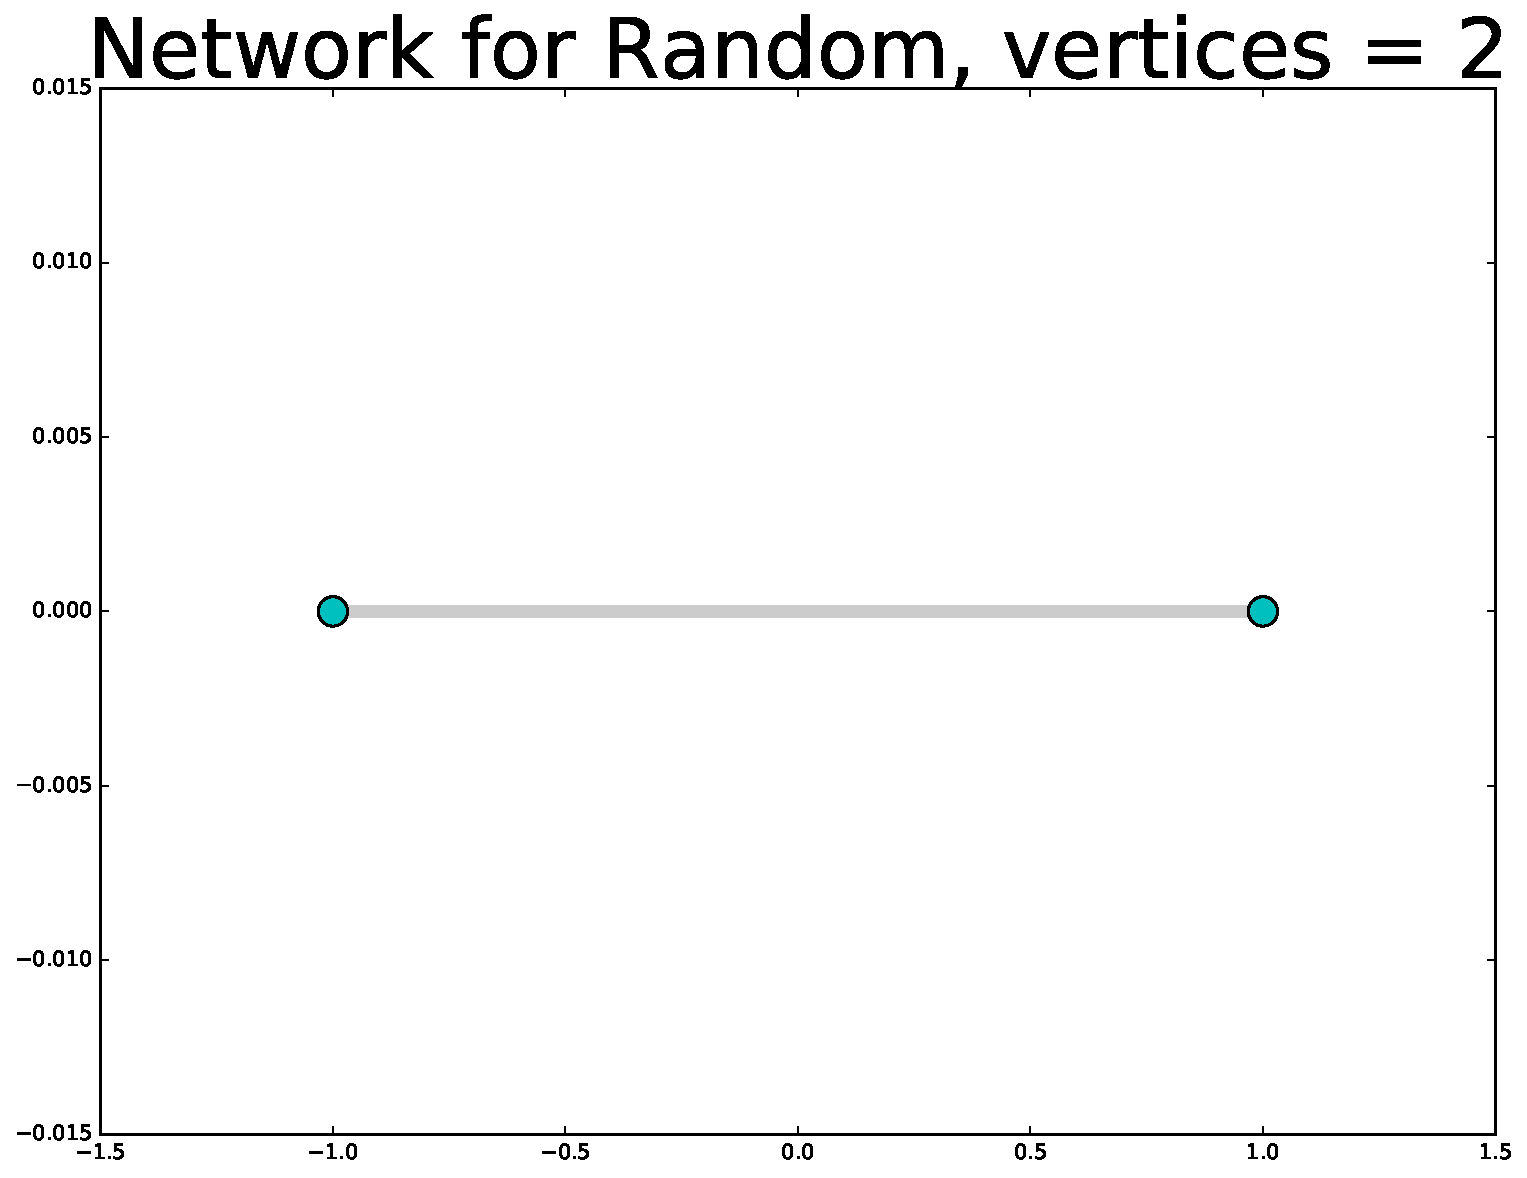
\includegraphics[width=\linewidth]{chapter-four/random_2.pdf}
		\caption{Two nodes}
	\end{subfigure}
	\hfill
	\begin{subfigure}[t]{0.30\textwidth}\centering
		\centering
		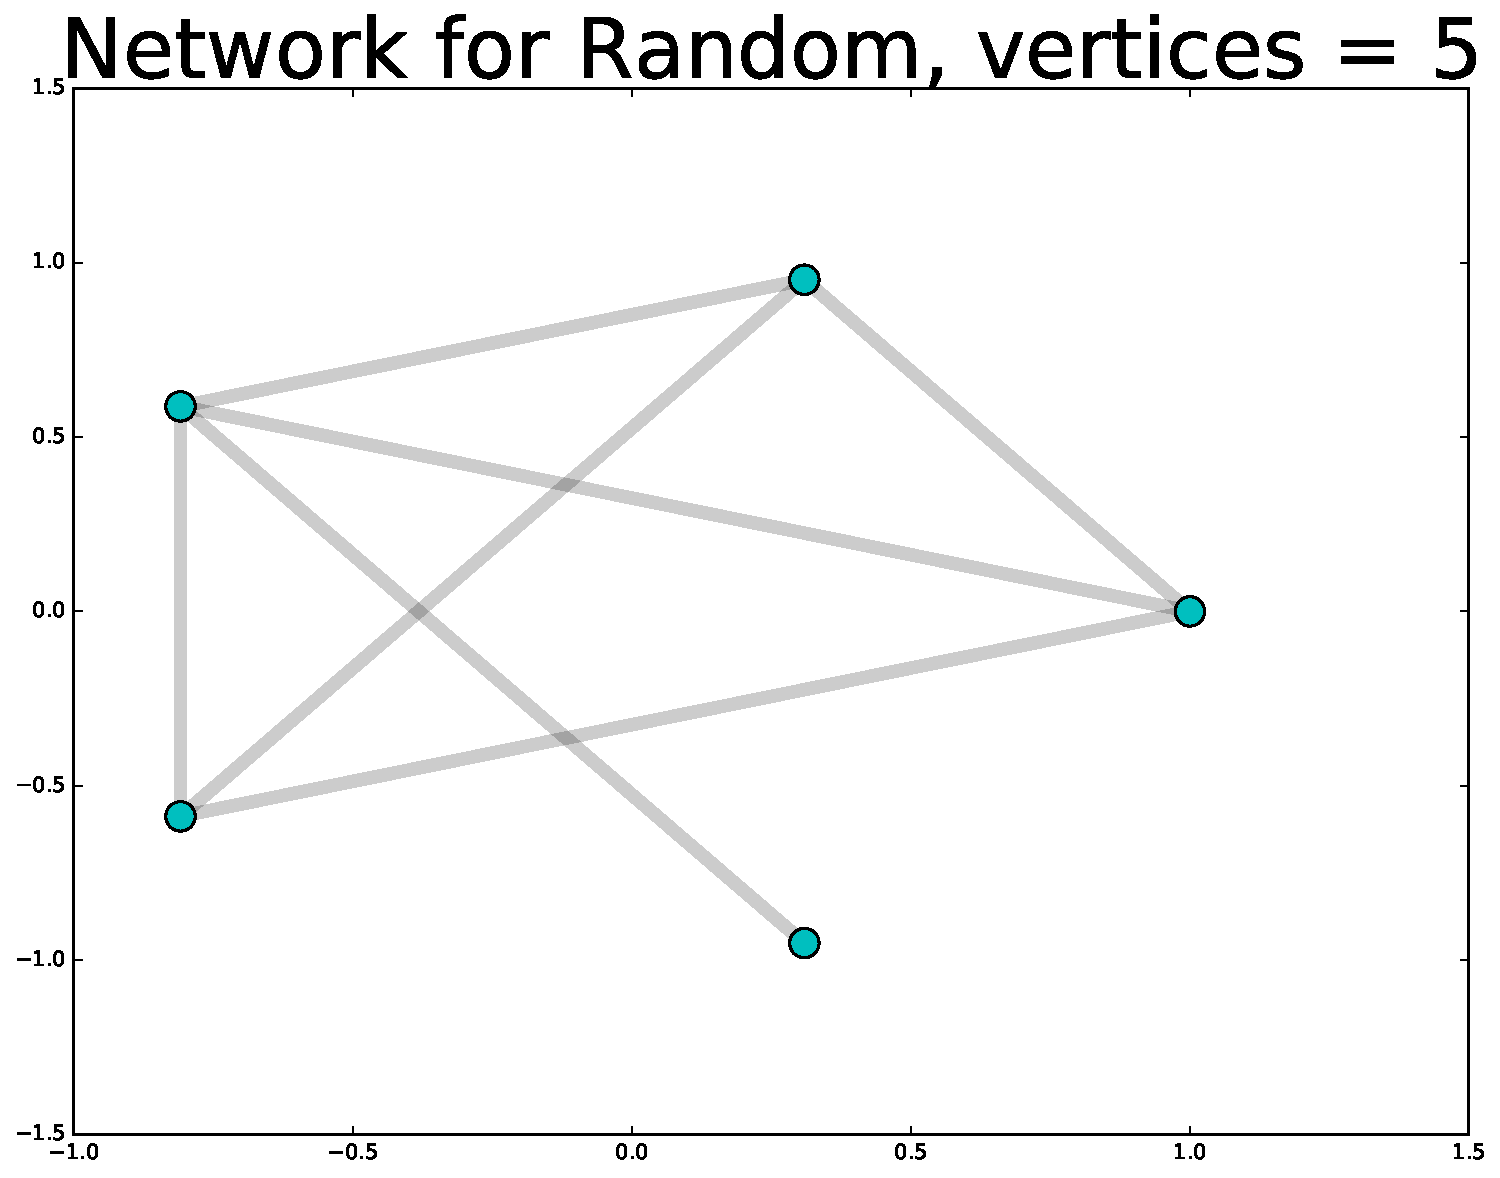
\includegraphics[width=\linewidth]{chapter-four/random_5.pdf}
		\caption{Five nodes}
	\end{subfigure}
	\hfill
	\begin{subfigure}[t]{0.30\textwidth}\centering
		\centering
		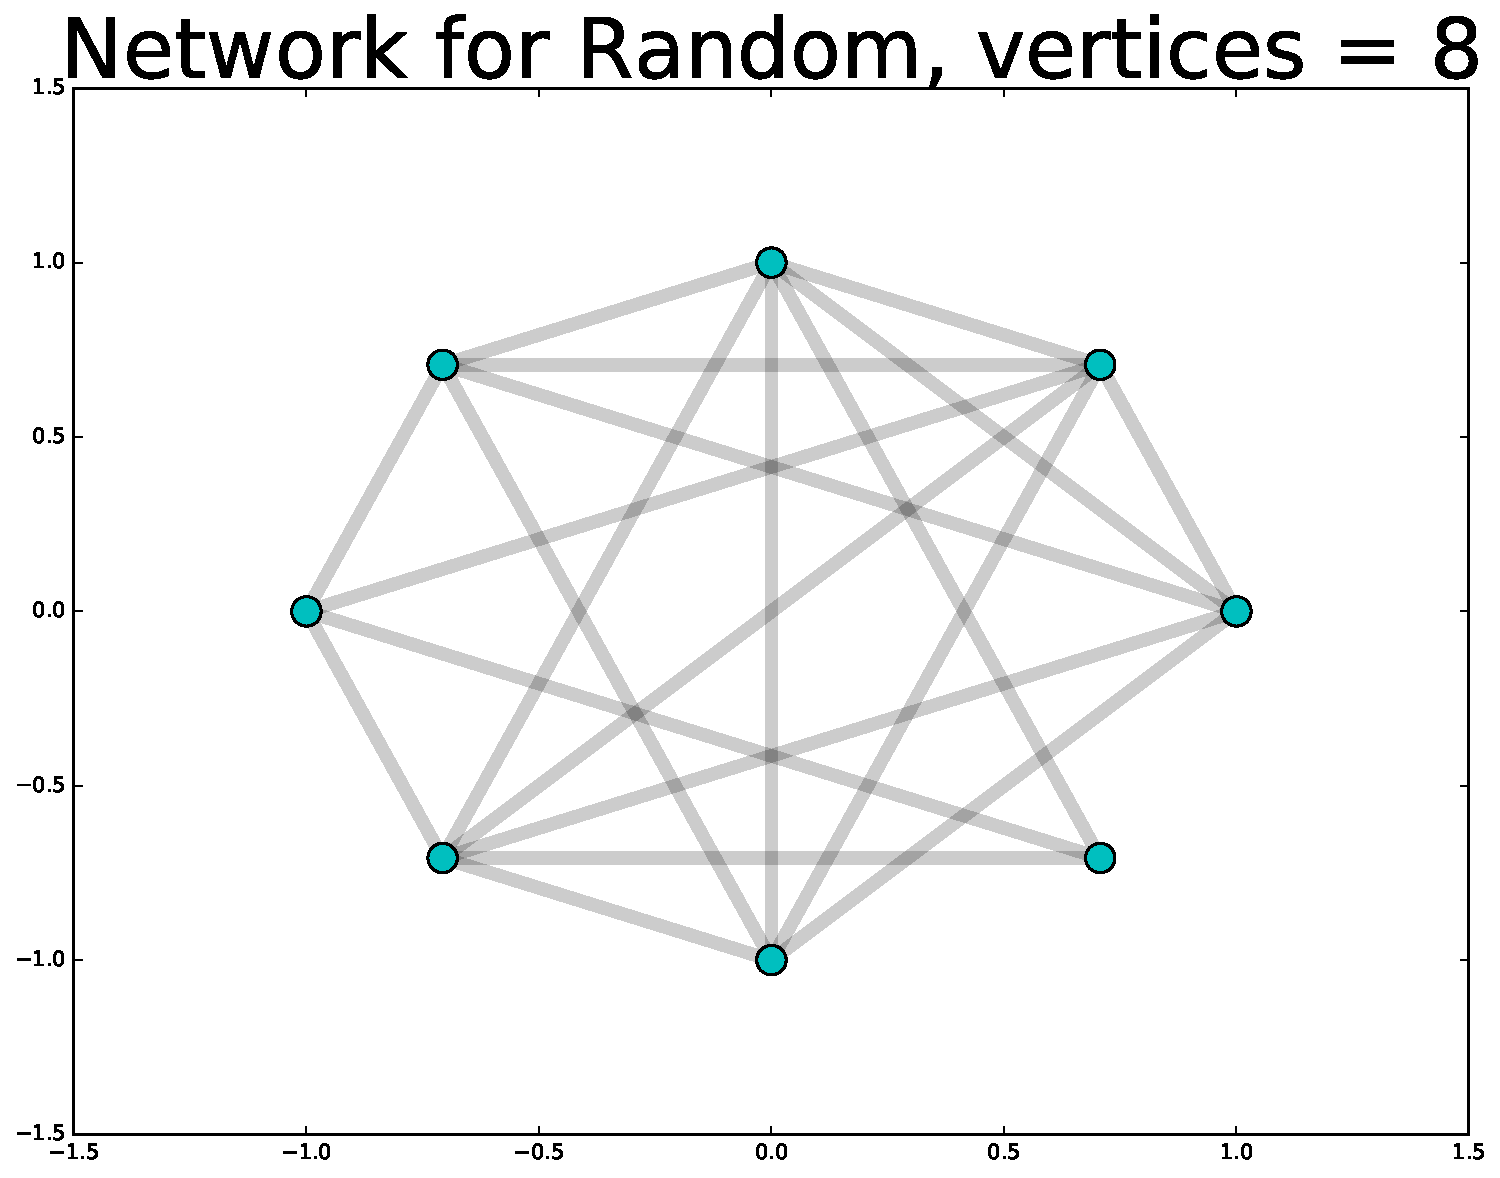
\includegraphics[width=\linewidth]{chapter-four/random_8.pdf}
		\caption{Eight nodes}
	\end{subfigure}
	\hfill
	\begin{subfigure}[t]{0.30\textwidth}\centering
		\centering
		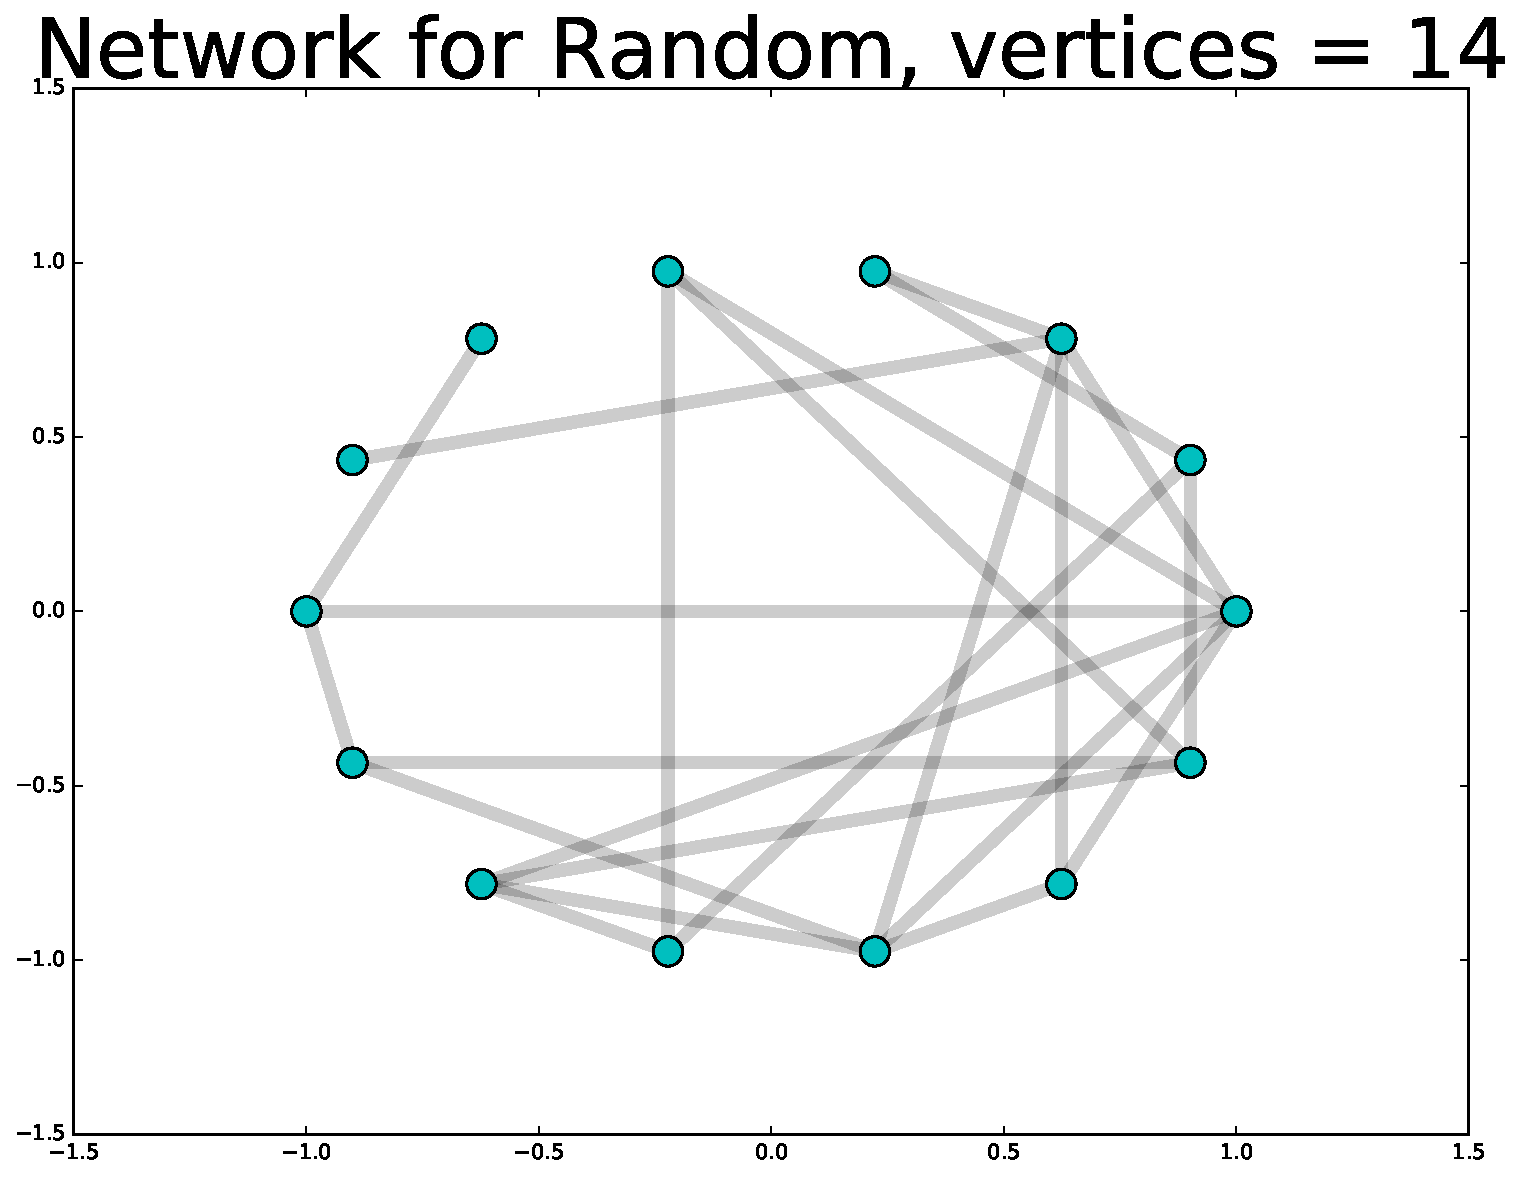
\includegraphics[width=\linewidth]{chapter-four/random_14.pdf}
		\caption{Fourteen nodes}
	\end{subfigure}
	\hfill
	\begin{subfigure}[t]{0.30\textwidth}\centering
		\centering
		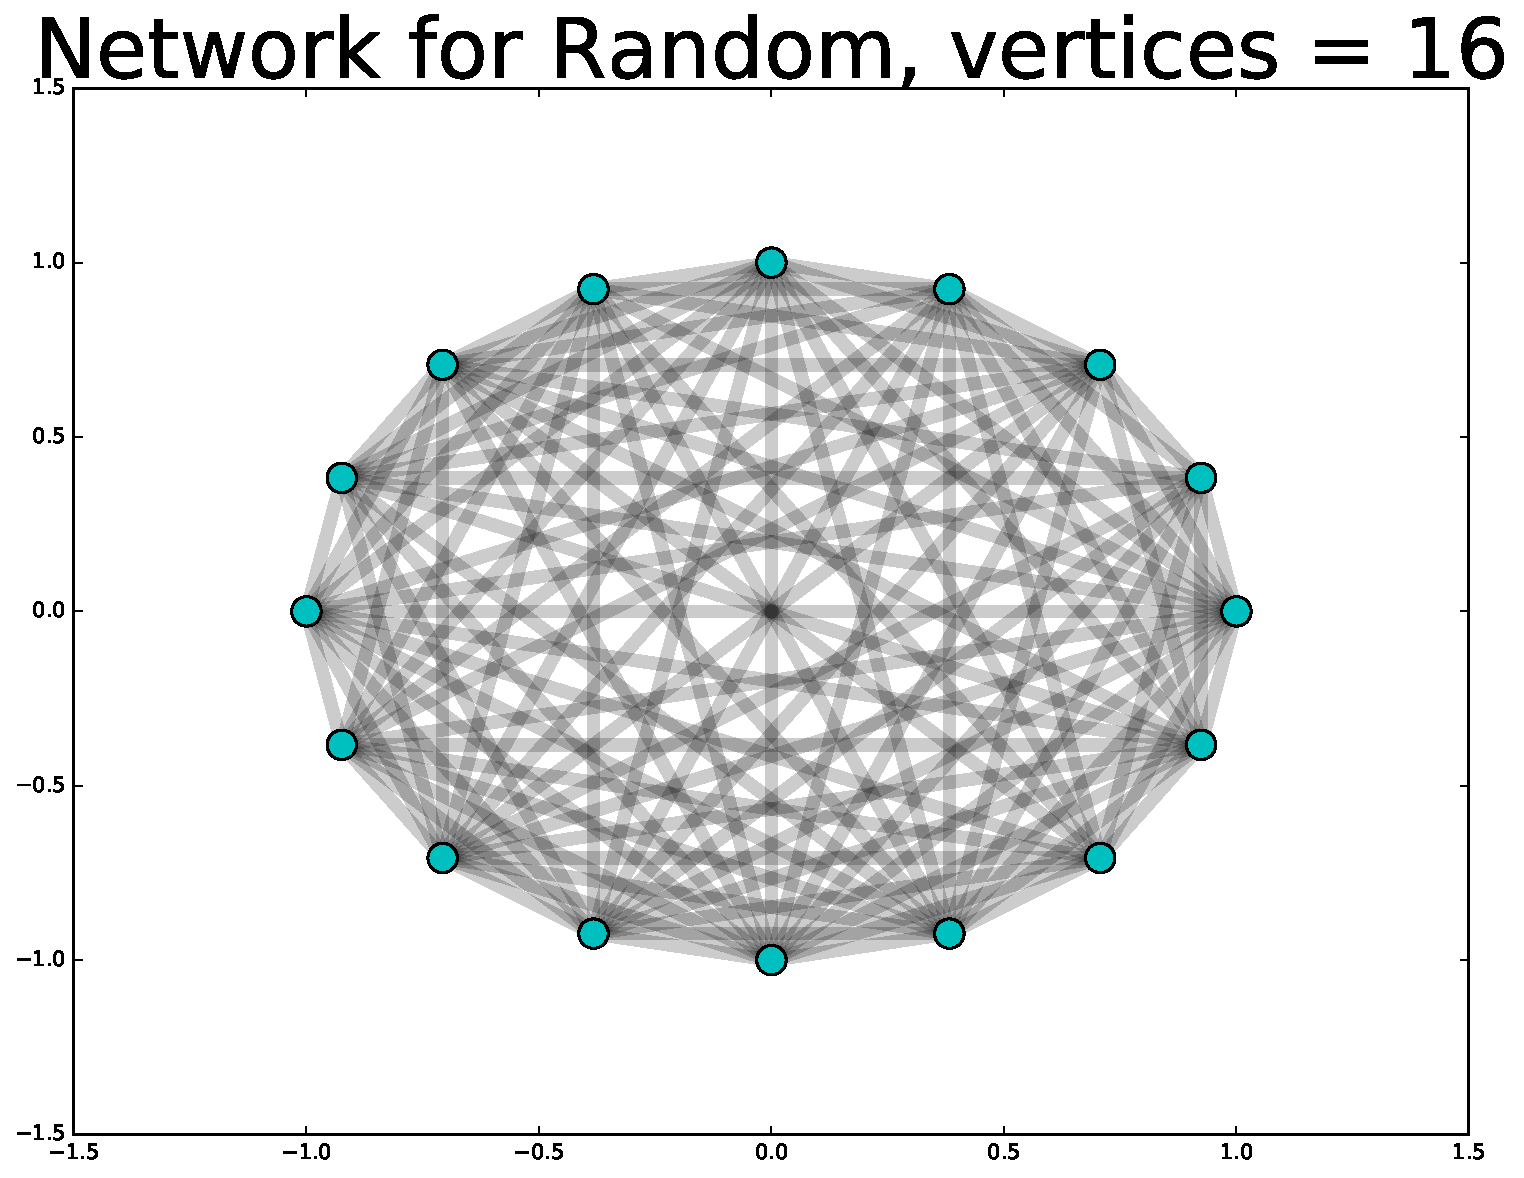
\includegraphics[width=\linewidth]{chapter-four/random_16.pdf}
		\caption{Sixteen nodes}
	\end{subfigure}
	\hfill
	\begin{subfigure}[t]{0.30\textwidth}\centering
		\centering
		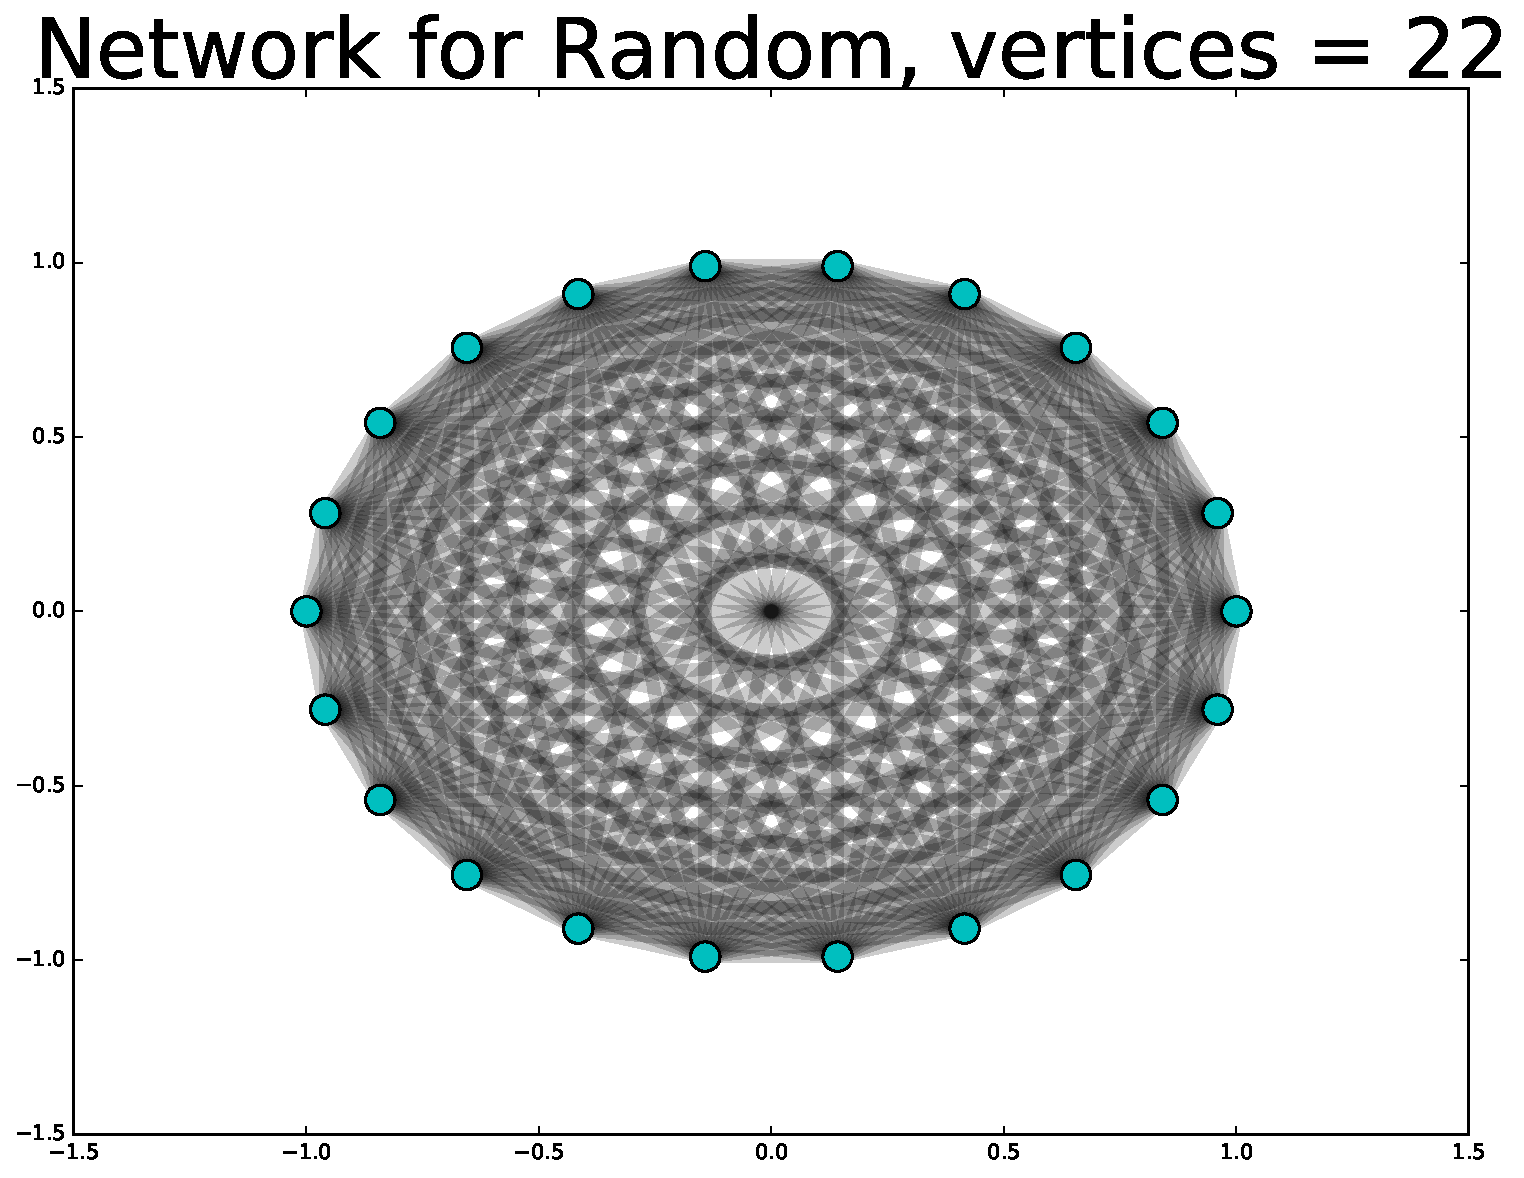
\includegraphics[width=\linewidth]{chapter-four/random_22.pdf}
		\caption{Twenty-two nodes}
	\end{subfigure}
	\caption{Various Erd\"{o}s R\'{e}nyi networks}
	\label{random_networks_illustration}
\end{figure}

To conclude, the complete networks method was the only method where tournament
of 50 players have been played. A total of 500 tournaments, with complete topology,
have been constructed and played through. Table~\ref{table:complete-summary-table}
summarizes, a few of the networks measures. For the complete networks, the measures
could have been predicted, due to the 'all connected rule'. The connectivity
coefficient is equal to the degree. They vary from 1 to 49. One degree value
corresponds to the first network, with a minimum number of nodes 2, and 49 to
the last networks, with a maximum number of 50 nodes.

\begin{table}[!hbtp]
	\centering
	\begin{adjustbox}{width=0.5\textwidth}
		\small
		\begin{tabular}{cccccccccc}
				\toprule
			\multicolumn{5}{|c|}{Complete Networks Summary Table}                     \\ \hline
			     & connectivity & clustering & degree & nodes                  \\ \hline
			mean & 32.70        & 0.99       & 32.70  & 33.70                  \\ \hline
			std  & 11.87        & 0.03       & 11.87  & \multicolumn{1}{c}{-} \\ \hline
			min  & 1.00         & 0.00       & 1.00   & 2.00                   \\ \hline
			max  & 49.00        & 1.00       & 49.00  & 50.00                  \\ \bottomrule
		\end{tabular}
	\end{adjustbox}
	\caption{Complete summary table}
	\label{table:complete-summary-table}
\end{table}

The mean clustering coefficients is set at 0.99 Indicating strong clusters
throughout the experiment, an anticipated result. Furthermore, eight random
graphs are displayed in Figure~\ref{complete_networks_illustration}.

\begin{figure}[!hbtp]
	\centering
	\begin{subfigure}[t]{0.30\textwidth}
		\centering
		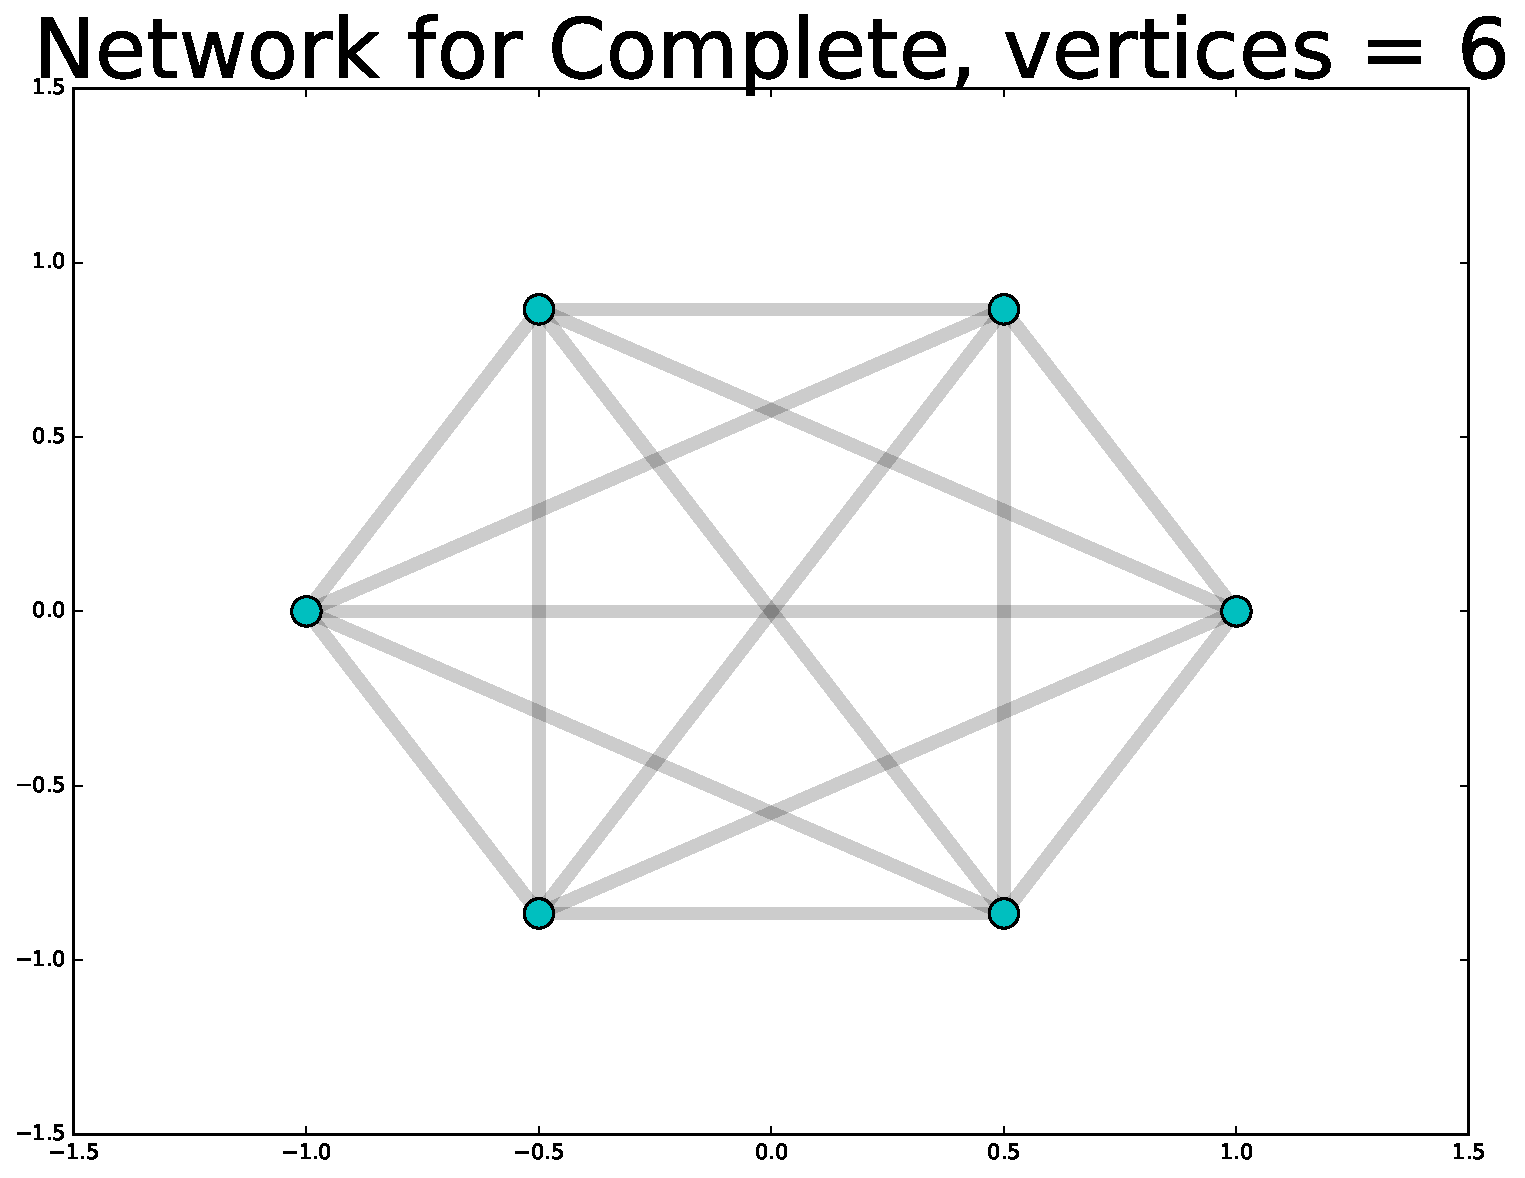
\includegraphics[width=\linewidth]{chapter-four/complete_6.pdf}
		\caption{Six nodes}
	\end{subfigure}
	\hfill
	\begin{subfigure}[t]{0.30\textwidth}\centering
		\centering
		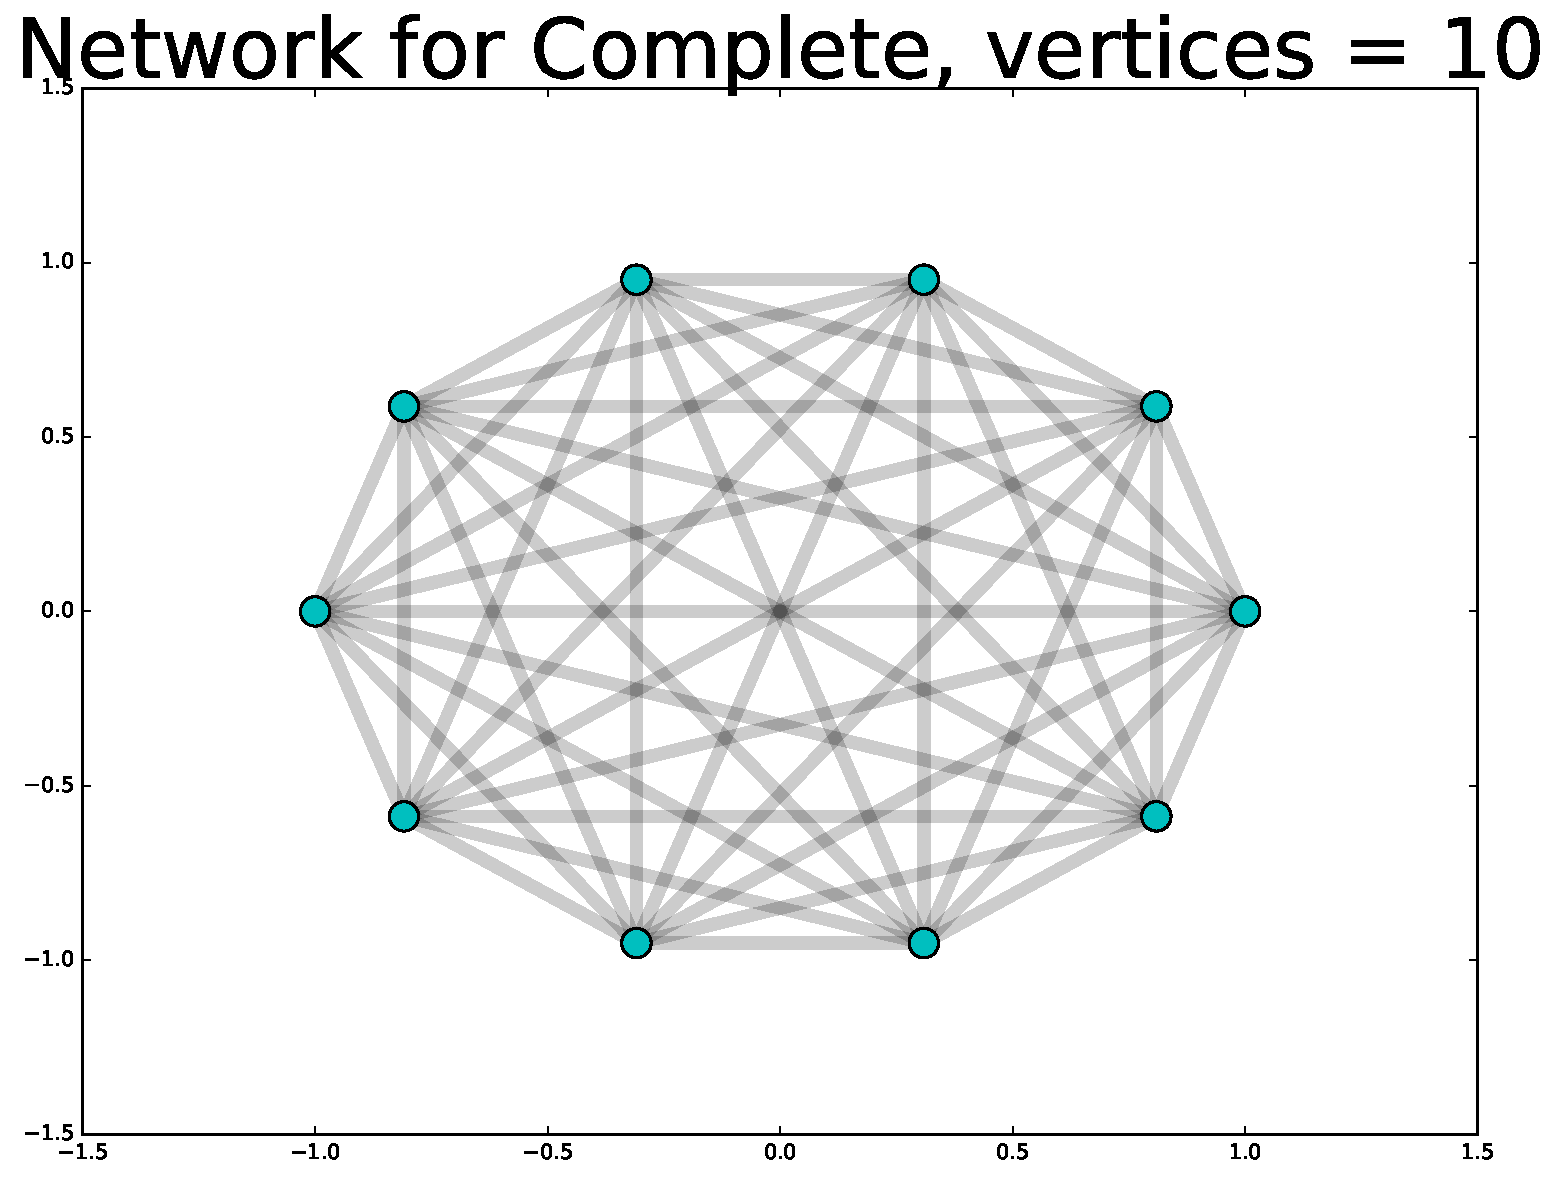
\includegraphics[width=\linewidth]{chapter-four/complete_10.pdf}
		\caption{Ten nodes}
	\end{subfigure}
	\hfill
	\begin{subfigure}[t]{0.30\textwidth}\centering
		\centering
		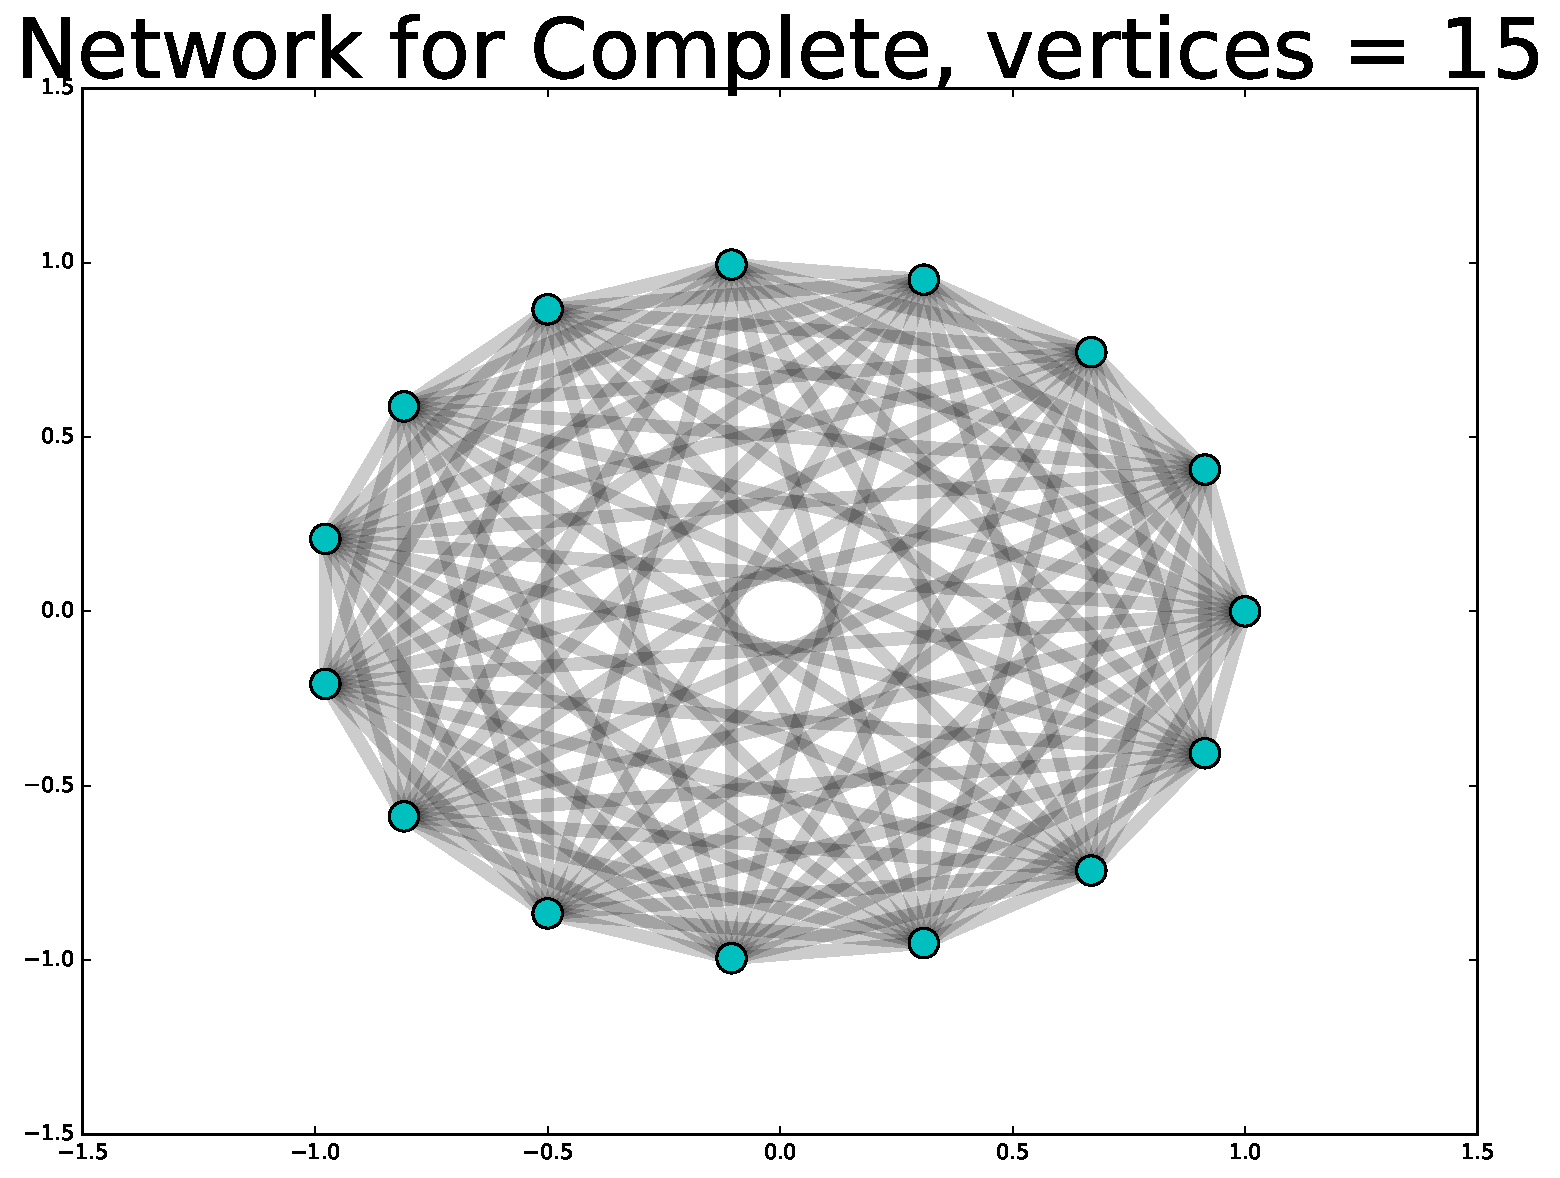
\includegraphics[width=\linewidth]{chapter-four/complete_15.pdf}
		\caption{Fifteen nodes}
	\end{subfigure}
	\hfill
	\begin{subfigure}[t]{0.30\textwidth}\centering
		\centering
		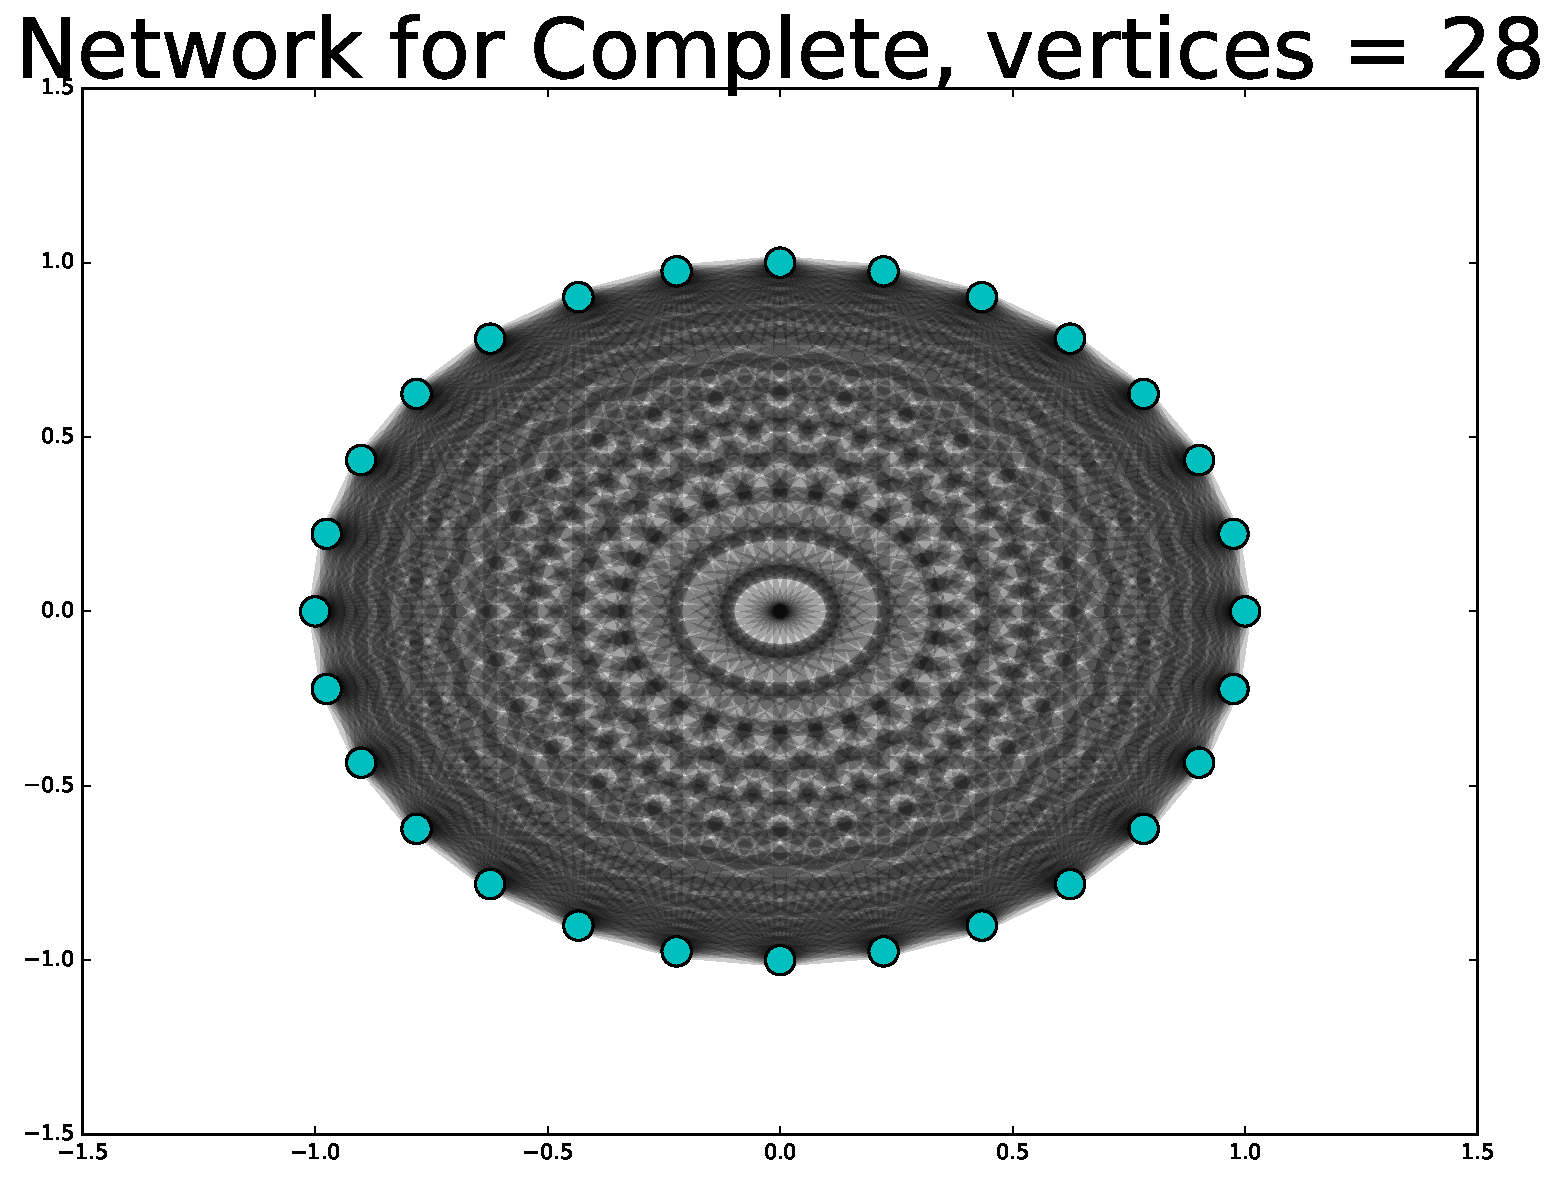
\includegraphics[width=\linewidth]{chapter-four/complete_28.pdf}
		\caption{Twenty-eight nodes}
	\end{subfigure}
	\hfill
	\begin{subfigure}[t]{0.30\textwidth}\centering
		\centering
		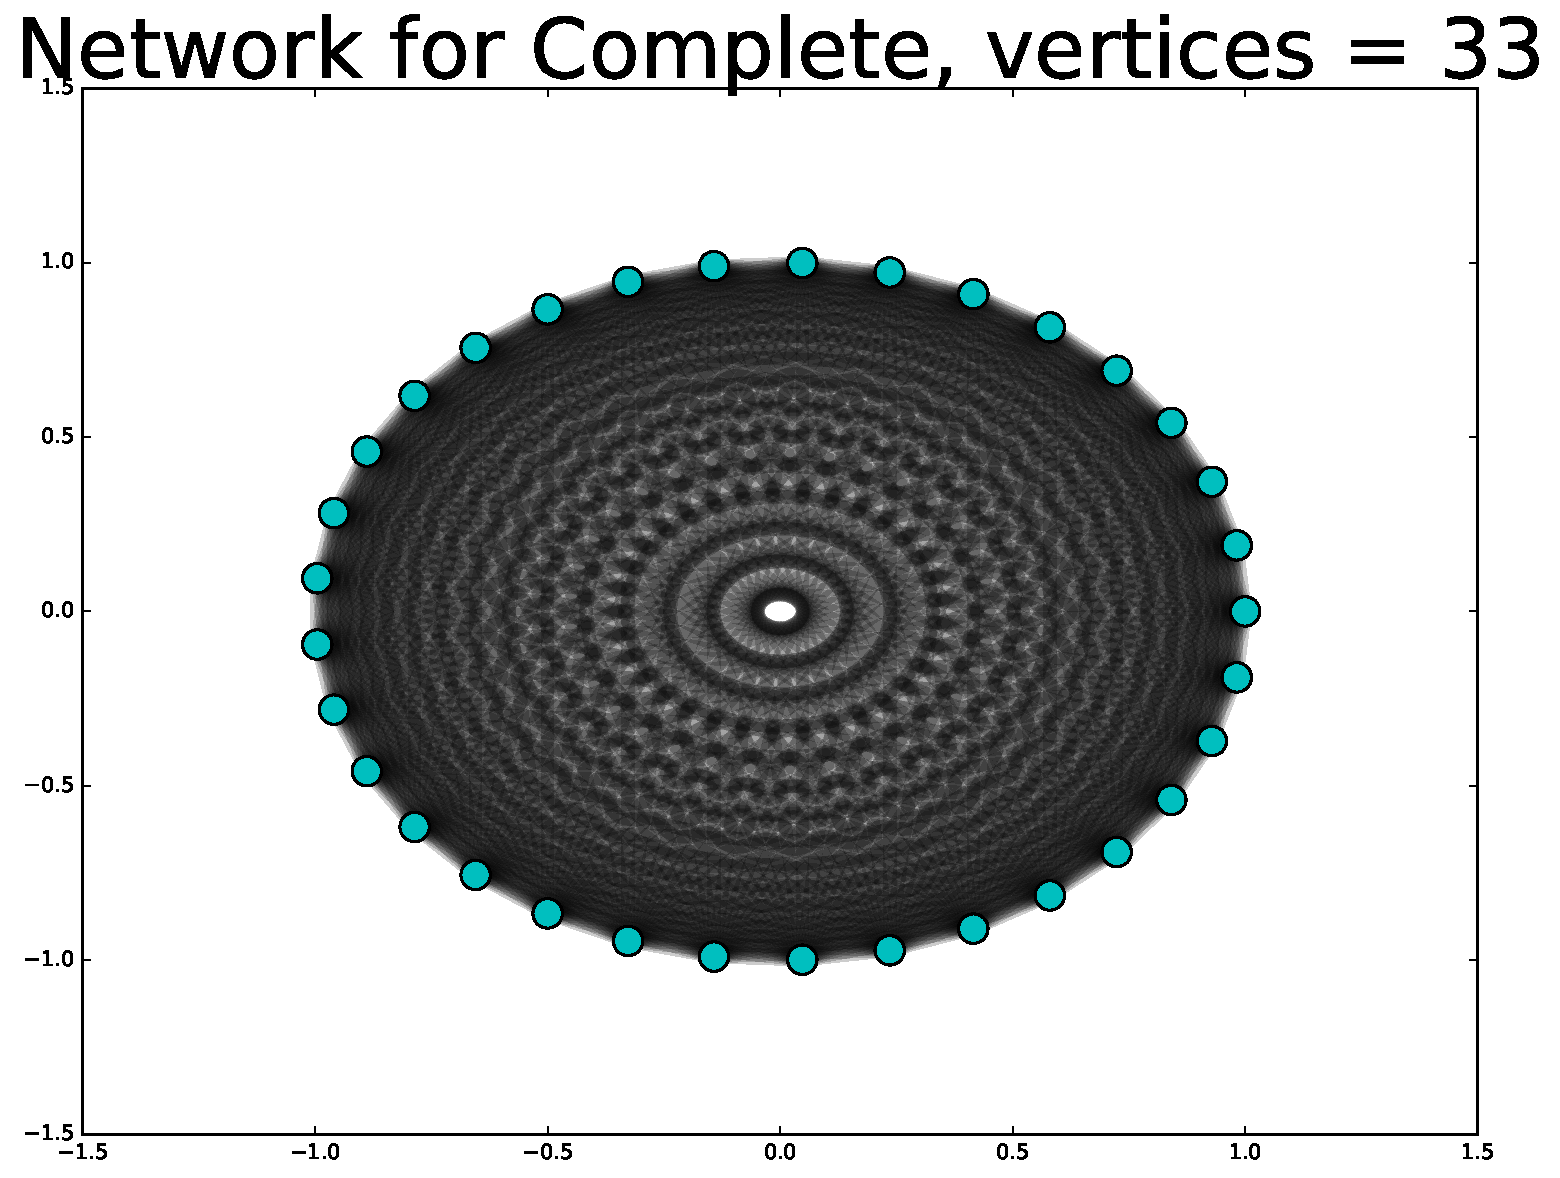
\includegraphics[width=\linewidth]{chapter-four/complete_33.pdf}
		\caption{Thirty-three nodes}
	\end{subfigure}
	\hfill
	\begin{subfigure}[t]{0.30\textwidth}\centering
		\centering
		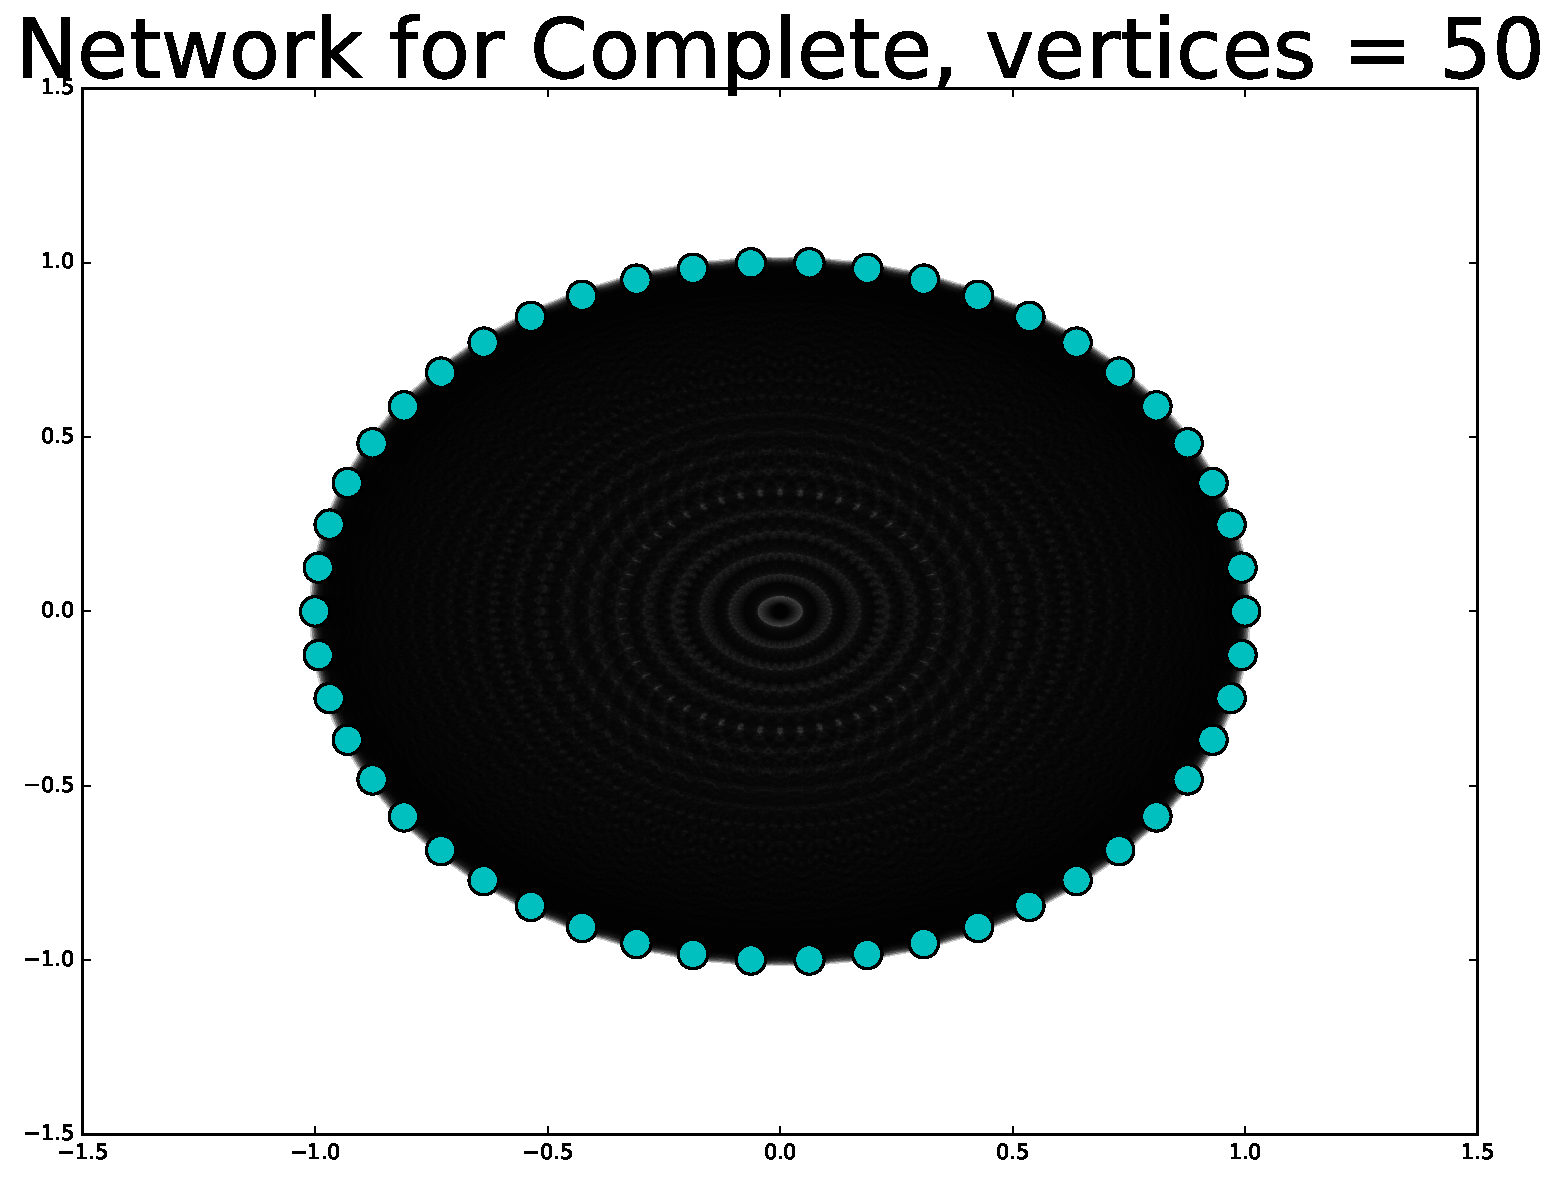
\includegraphics[width=\linewidth]{chapter-four/complete_50.pdf}
		\caption{FIfty nodes}
	\end{subfigure}
	\caption{Various Complete networks}
	\label{complete_networks_illustration}
\end{figure}

In this subsection, an initial summary of the overall graphs conducted, in
each of the methods has been held. The number of tournaments, as well as the
tournament size differ. In the following subsection, an initial analysis on the
data produced by each of these methods individually is held.

\subsection{Data Analysis}
This subsection summarizes the results of the tournaments that have been extracted
for the methods.
Individual tables have been managed for each method. The payoff matrix, for
the game of the prisoners dilemmas, follows the payoffs as explained in~\autoref{sub:prisoner-dilemma}.
Thus, punishment payoff is equal to 1 temptation to 5, reward is equal to 3 and
the sucker's payoff is set to 0.

For the small word method the description of the average score, average
neighborhood score, cooperating ratio and neighborhood size are shown in
Table~\ref{table:summary-small-data}. The average score and average
neighborhood score, are fairly equal, both ranging from 0 ($e$, $pi$) to 5 (Fool Me Forever, Bully)
with an average of 2.4. The mean cooperation rating, is equal to 0.64. Thus, strategies behave mostly cooperative.
Mean neighborhood size is 4, which is agreement with~\autoref{sub:network-analysis}.
Maximum neighbors is 9, so even if the maximum players has been 11, no strategy
compete against 10 strategies.

\begin{table}[!hbtp]
	\centering
	\begin{adjustbox}{width=0.8\textwidth}
		\small
		\begin{tabular}{cccccccccc}
				\toprule
			\multicolumn{5}{|c|}{Small world Data Summary Table}                                \\ \hline
			     & average score & average neighborhood & cooperating ratio & neighborhood size \\ \hline
			mean & 2.40          & 2.40                 & 0.64              & 4.74              \\ \hline
			std  & 0.63          & 0.40                 & 0.30              & 2.65              \\ \hline
			min  & 0.00          & 0.00                 & 0.00              & 1.00              \\ \hline
			max  & 5.00          & 5.00                 & 1.00              & 12.00             \\ \bottomrule
		\end{tabular}
	\end{adjustbox}
	\caption{Small world Data Summary Table}
	\label{table:summary-small-data}
\end{table}

For the random method, Table~\ref{summary-random-data} is an initial summary,
for basic measures of the tournaments. Similarly, the average score and average
neighborhood score, are fairly equal. This time, the average neighborhood score,
is slightly lower, 2.38. The minimum average score achieved is 0 ($phi$, $e$, Cycle Hunter)
and the maximum 4.99, again by $e$ and $phi$. Obviously these average scores were achieved in
different tournaments. The mean cooperating ratio, is higher than 0.50.
Thus, strategies tend to cooperate and the neighborhood size, verifies the results
of ~\autoref{sub:network-analysis}.

\begin{table}[!hbtp]
	\centering
	\begin{adjustbox}{width=0.8\textwidth}
		\small
		\begin{tabular}{cccccccccc}
				\toprule
			\multicolumn{5}{|c|}{Random Data Summary Table}                                      \\ \hline
			     & average score & average neighborhood & cooperating ratio & neighborhood size \\ \hline
			mean & 2.38          & 2.38                 & 0.63              & 11.00             \\ \hline
			std  & 0.44          & 0.24                 & 0.25              & 6.57              \\ \hline
			min  & 0.00          & 0.06                 & 0.00              & 1.00              \\ \hline
			max  & 5.00          & 4.99                 & 1.00              & 28.00             \\ \bottomrule
		\end{tabular}
	\end{adjustbox}
	\caption{Random Data Summary Table}
	\label{summary-random-data}
\end{table}

Finally, for the complete experiment, Table ~\ref{table:summary-complete-data}. The
average scores, are lower for this experiment. Both mean average scores are
equal to 2.38. But the maximum average scores, strategies and neighbors, are
below 4. On the other hand, the minimum score are non zero. Specifically,
the minimum average score is equal to 0.55 (Cycler CCD) and the maximum 3.98, Calculator.
The behavior of the scores can be explained by the topology. In the complete topology experiment,
the highest number of games are played. Considering that for each tournament
\(n-1\) games take place. Thus, scoring zero is less likely, because the games
you play are increased by far, and the overall score falls for the same reason.
Cooperating ratio, has a mean value of 0.63 and the neighborhood size
verify what was discussed in ~\autoref{sub:network-analysis}.

\begin{table}[!hbtp]
	\centering
	\begin{adjustbox}{width=0.8\textwidth}
		\small
		\begin{tabular}{cccccccccc}
				\toprule
			\multicolumn{5}{|c|}{Complete Data Summary Table}                                      \\ \hline
			     & average score & average neighborhood & cooperating ratio & neighborhood size \\ \hline
			mean & 2.38          & 2.38                 & 0.63              & 32.70             \\ \hline
			std  & 0.35          & 0.13                 & 0.23              & 11.90             \\ \hline
			min  & 0.55          & 0.54                 & 0.00              & 1.00              \\ \hline
			max  & 3.89          & 3.58                 & 1.00              & 49.00             \\ \bottomrule
		\end{tabular}
	\end{adjustbox}
	\caption{Complete Data Summary Table}
	\label{table:summary-complete-data}
\end{table}

This section has been a preliminary analysis on the outcomes produced by
the three methods. In the upcoming section, more important topics are
raised and an analysis on performance is undertaken.

\section{Performance Analysis}
\label{performance-analysis}
In this section, three measure will be scrutinized, to assess performance of the
strategies. These measures are the winning ratio, the normalized average score
and the median rank. Before hands, the strategies are categorized based on their
average cooperating ratio and the network attributes to which they compete in. Moreover,
various regression models have been constructed for the median rank, and lastly,
the findings are summarized.

\section{Classification}
\label{sub:classification}
For being able to conduct the analysis on performance two classifications are
being performed. The two classification that will be conducted are based on:
\begin{itemize}
	\item The average cooperating ratio of the strategies
	\item The networks connectivity and clustering coefficients on the networks
	      used for the spatial tournaments.
\end{itemize}

This is done for the two following reasons. Firstly, as stated in~\autoref{chap:Two},
the Axelrod-Python library (version 1.7.0), consists of 132. Reading though
the documentation for each strategy to distinguish any similarities between
the strategies, would be a challenging task. For this reason, the average cooperation
rating will be used to classify the strategies into categories. Thus, strategies
in the same category will be characterized as similar, based on their level of
cooperation. Secondly, because the performance of the strategies needs to be assessed
based on the topology of the spatial tournament, but networks used itself does
not matter, the clustering and cooperation coefficient are used for a 2 dimensional
clustering.

The clustering will be performed using the popular \(k\)-means algorithm~\cite{kmeans}.
\(k\)-means aims to store observations to k clusters. It stores k centroids
that it used to define cluster. An observation is considered to be in a
particular cluster if it is closer to that cluster's centroid than any other
centroid. The best centroids are identified by:
\begin{itemize}
	\item assigning data points to clusters based on the current centroids
	\item choosing centroids (points which are the center of a cluster) based on
	      the current assignment of data points to clusters.
\end{itemize}

For the average cooperation, five individual categories have been created.
The boundaries of each class and the number of strategies in each category
can been seen in Table~\ref{table:class}, a more detailed table, with the respective category of each
strategy can be found in the Appendix~\ref{append:class-categories}.

Overall six strategies are in the low category. Their average cooperating ration
ranges between 0.00 and 0.20. In the weak category, the ratio is between
0.23 and 0.40, and is consisted of 17 strategies. 28 strategies are
in the mid category, with upper bound of ratio 0.57 and lower bound a 0.42.
The moderate category, is for strategies which ratio is between 0.58 and 0.75.
Lastly, the high category, with 48 strategies and a mean ratio of 0.87.

\begin{table}[H]
	\centering
	\begin{adjustbox}{width=0.4\textwidth}
		\small
		\begin{tabular}{cccccccccc}
				\toprule
			\multicolumn{5}{|c|}{Classification Table}                        \\ \hline
			Categories & count & \multicolumn{3}{l}{cooperating ratio}        \\ \hline
			         &    & min  & mean & max  \\ \hline
			low      & 6  & 0.00 & 0.10 & 0.20 \\ \hline
			weak     & 17 & 0.23 & 0.32 & 0.40 \\ \hline
			mid      & 28 & 0.42 & 0.50 & 0.57 \\ \hline
			moderate & 33 & 0.58 & 0.65 & 0.75 \\ \hline
			high     & 48 & 0.76 & 0.87 & 1.00 \\ \bottomrule
		\end{tabular}
	\end{adjustbox}
	\caption{Classification table for cooperating ratio}
	\label{table:class}
\end{table}

Applying a 2 dimensional \(k\)-means algorithm to the data, for connectivity and
clustering, returns the following clusters, shown in Table~\ref{table:clusters}.
4 different classes have been created, with means 0.00, 1.00, 2.00 and 3.00 respectively.
In the scatter plot illustrated in Figure~\ref{fig:clusters}, it is clear that only connectivity
affects the means of the clusters. Thus the categories have been named after
the level of connectivity. High connectivity consists of 8100 observations,
moderate connectivity of 75649 observation. Lastly, mid connectivity includes
242405 participants and low connectivity 596259.

\begin{table}[!hbtp]
	\centering
	\begin{adjustbox}{width=0.7\textwidth}
		\small
		\begin{tabular}{cccccccccc}
				\toprule
			\multicolumn{5}{|c|}{Classification Table} \\ \hline
			Categories & number of observation & \multicolumn{3}{l|}{connectivity and clustering} \\ \hline
			                      &        & min  & mean & max  \\ \hline
			High connectivity     & 596259 & 0.00 & 0.00 & 0.00 \\ \hline
			Moderate connectivity & 242405 & 1.00 & 1.00 & 1.00 \\ \hline
			Mid connectivity      & 75649  & 2.00 & 2.00 & 2.00 \\ \hline
			Low connectivity      & 8100   & 3.00 & 3.00 & 3.00 \\ \bottomrule
		\end{tabular}
	\end{adjustbox}
	\caption{Classification table for network attributes}
	\label{table:clusters}
\end{table}

\begin{figure}[H]
	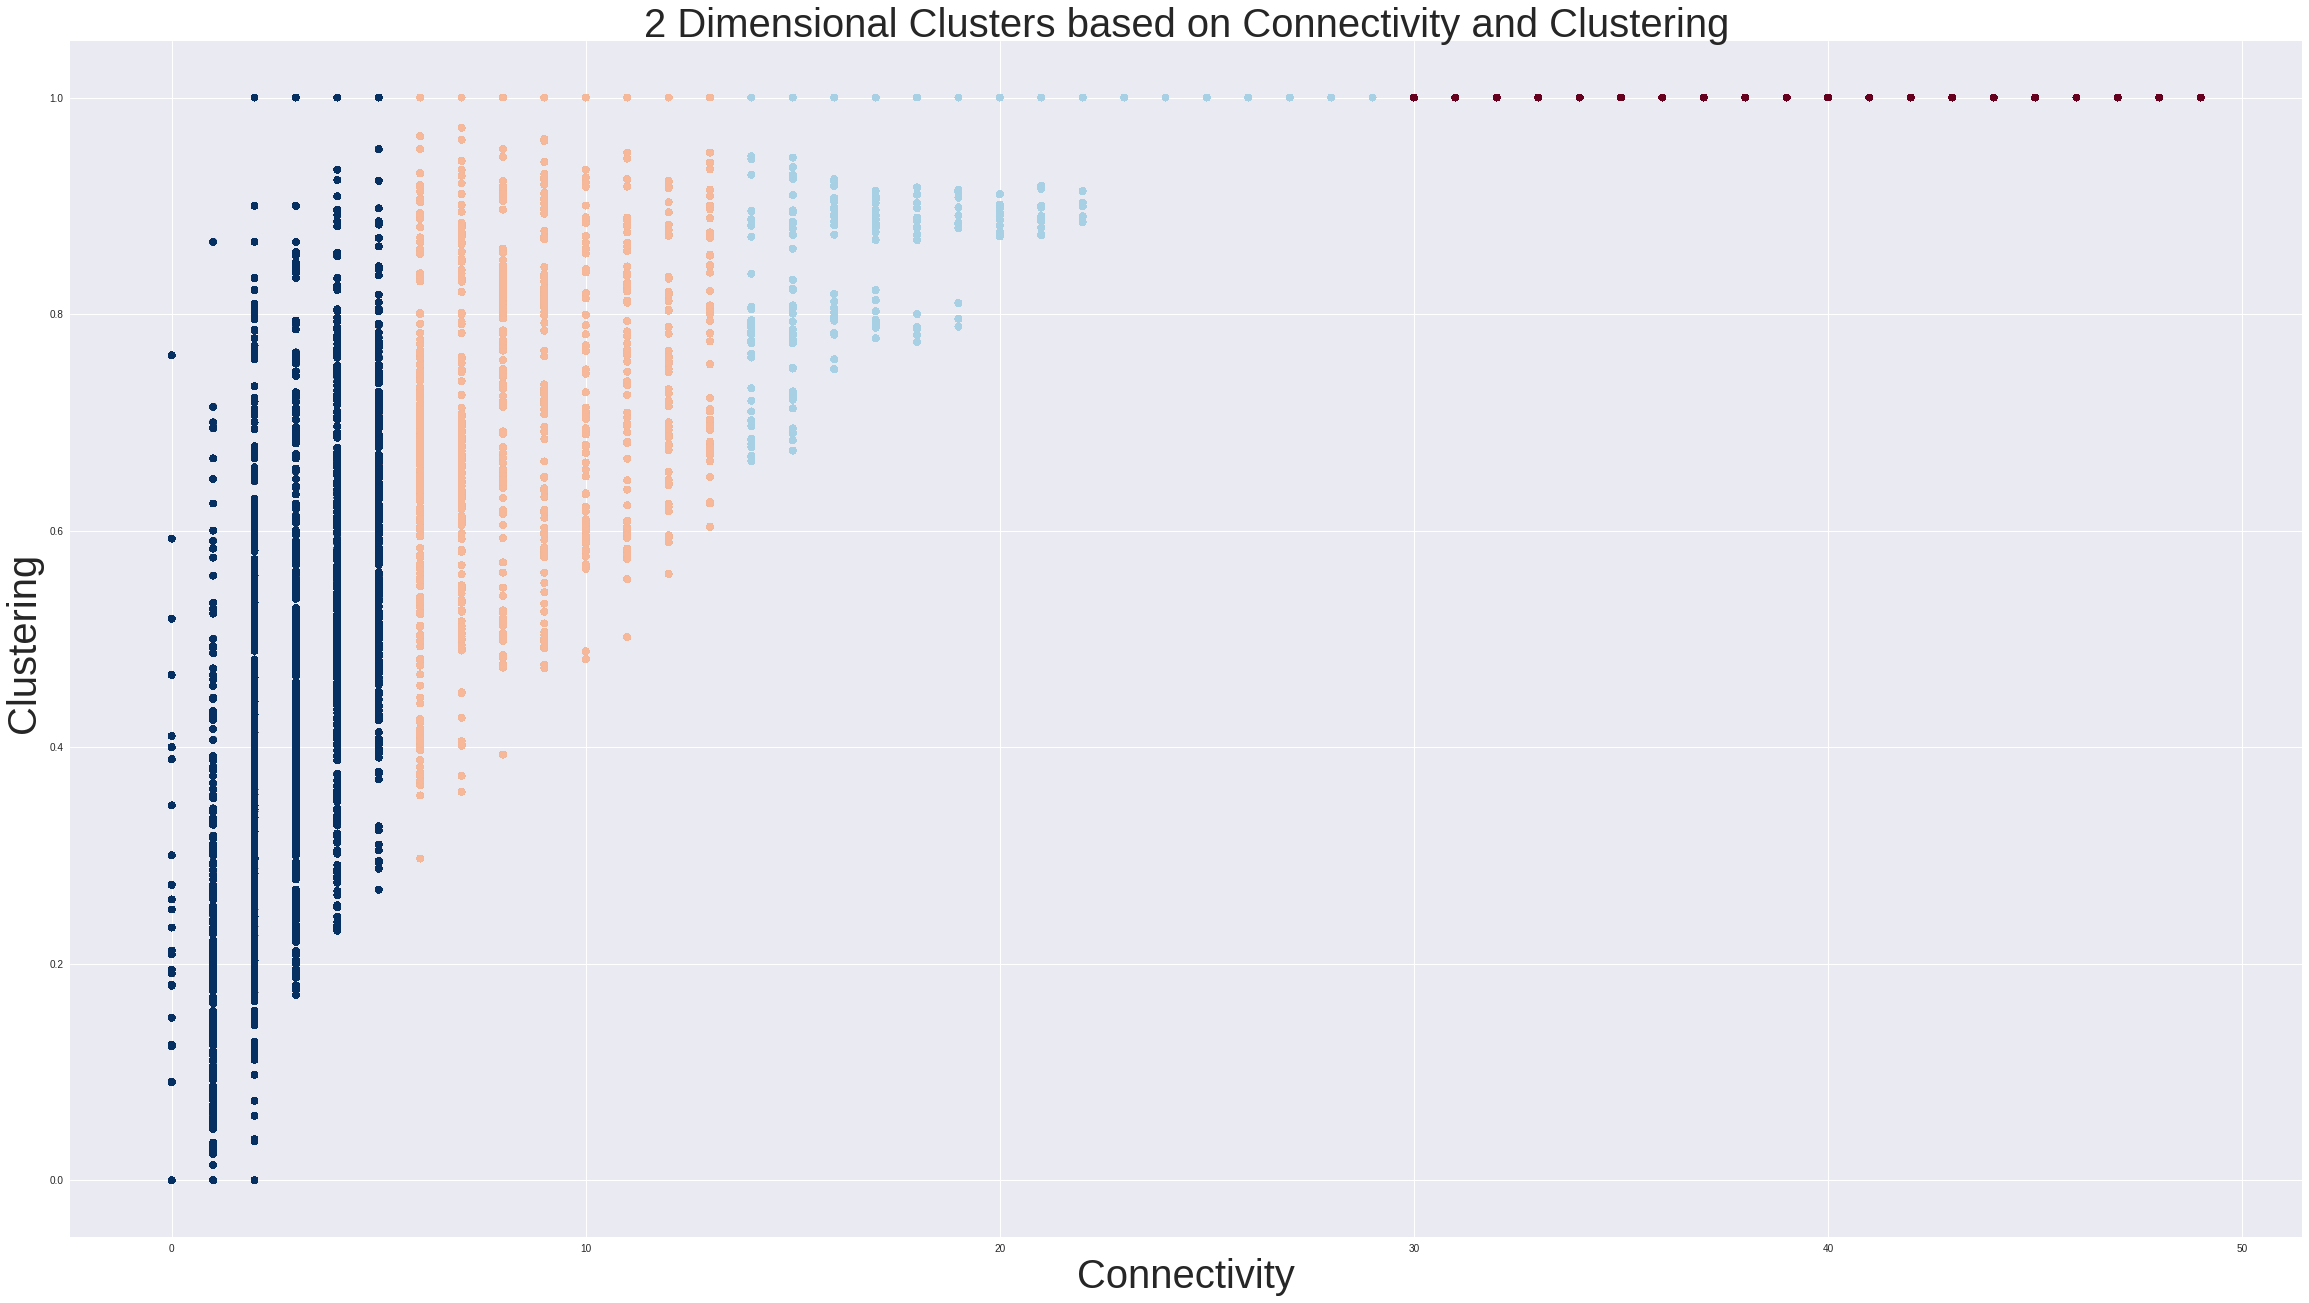
\includegraphics[width=1.2\linewidth,center]{chapter-four/index.png}
	\caption{Clusters based on connectivity and clustering coefficients}
	\label{fig:clusters}
\end{figure}

In this subsection the classification of the strategies and data have been
explained. The classification of the strategies will be a reliable tool
of similarity in the following subsections, and now that the network
attributes have been clusters they will be used further in the analysis.

\subsection{Winning Ratio}
In this subsection, the strategies are being assessed based on the winning ratio.
The strategies have been ranked, and Figure~\ref{fig:wining-second-gen}
illustrates the strategies with ascending order. The highest ranked strategies,
are:
\begin{itemize}
	\item Fool Me Forever, a high cooperative strategy, with a winning ratio of 0.178
	\item Grumpy, a high cooperative strategy, with a winning ratio of 0.179
	\item Ripoff, a mid cooperative strategy, with a winning ratio of 0.187
	\item Cycler DDC, a weak cooperative strategy, with a winning ratio of 0.203
	\item Calculator, a weak cooperative strategy, with a winning ratio of 0.228
\end{itemize}

Even though, Fool Me Forever, Grumpy, are characterized as highly
cooperatives strategies, Cycler DDC and Calculator are weak cooperators. The
strategies that have achieved zero wining ratio are listed here:
\begin{itemize}
	\item Fortress4, a low cooperative strategy
	\item Math Constant Hunter, a moderate cooperative strategy
	\item Win-Shift Lose-Stay, a mid cooperative strategy
	\item Once Bitten, a high cooperative strategy
	\item ThueMorseInverse, a mid cooperative strategy
	\item Retaliate (0.1), a moderate cooperative strategy
\end{itemize}

\begin{figure}[H]
	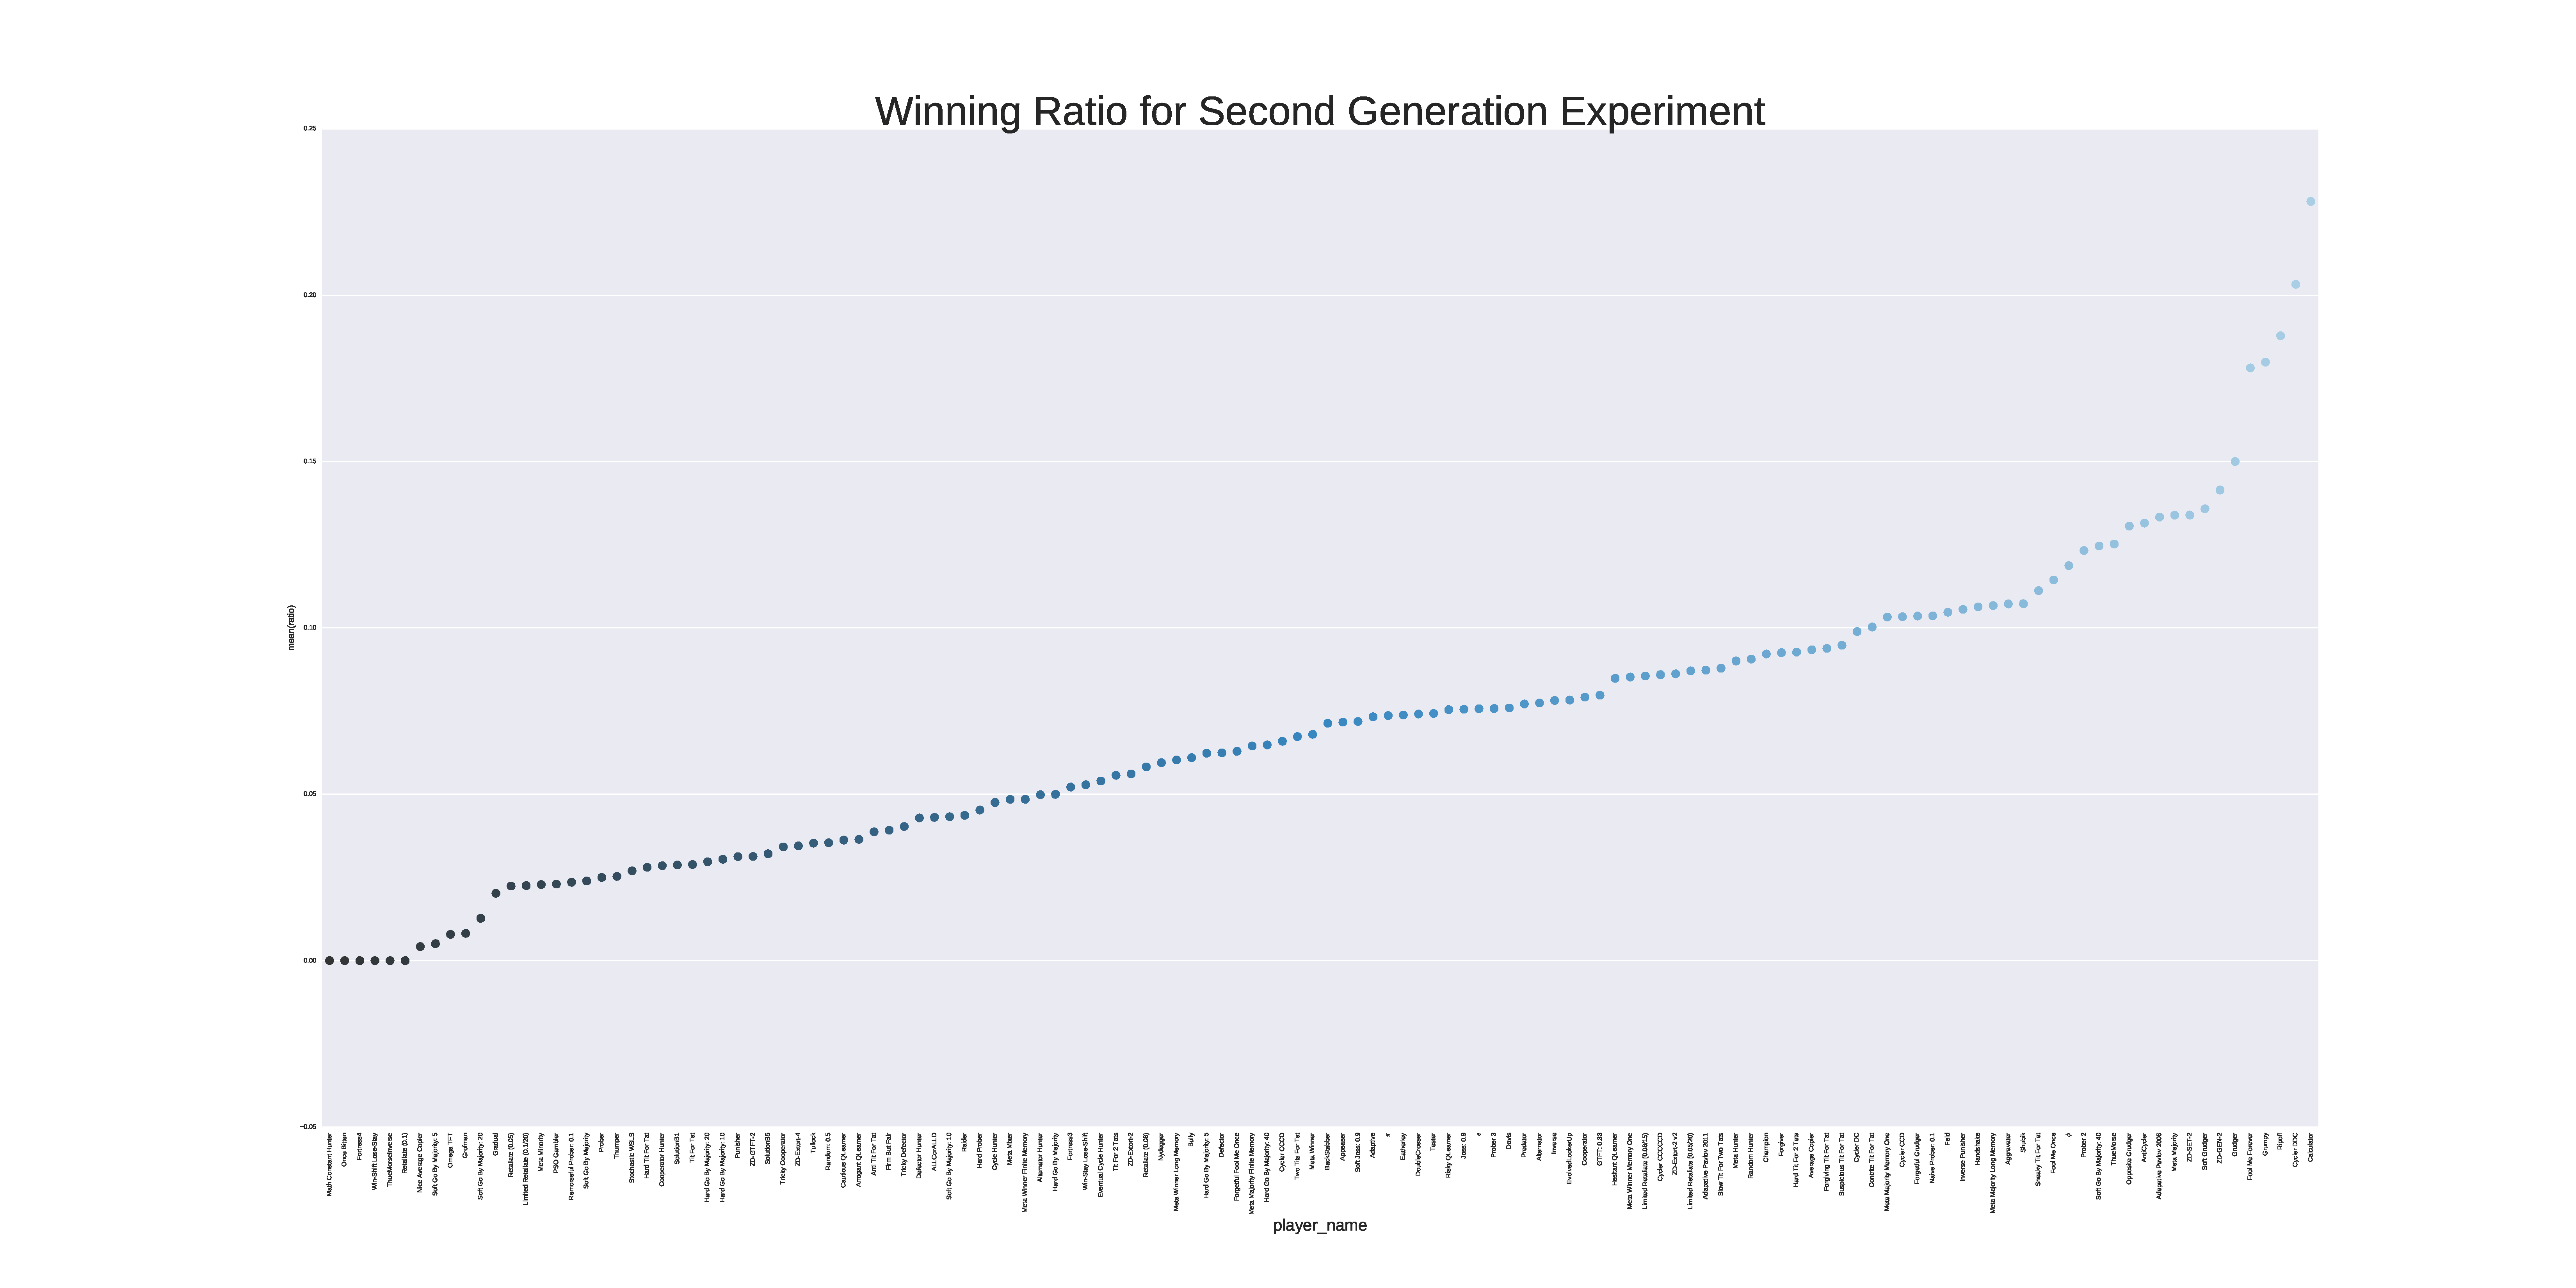
\includegraphics[width=1.2\linewidth,center]{chapter-four/winning-ratio.pdf}
	\caption{Ranks based on winning ratio}
	\label{fig:wining-second-gen}
\end{figure}

There seems to be no correlation between that winning ratio and the cooperation
categories. Furthermore, due the conclusion of ~\autoref{chap:Three}, winning ratio was described as
an non fitting performance measure. Thus, no more attention will be given to
winning ratio. In the following subsections, there is a briefly discussion of the
normalized average score and afterwards an in depth analysis on the normalized
ranking.

\subsection{Normalized Average Score}
\label{sub:chap-four-normalized-score}
In this subsection, the normalized average score is studied. The strategies
have been ranked based on their mean normalized score, and Figure~\ref{fig:wining-second-gen} illustrates
the ranks with ascending order. The highest ranked strategies have been:

\begin{itemize}
	\item PSO Gambler, a moderate cooperative strategy, with a mean score of 0.005386
	\item Win-Shift Lose-Stay, a mid cooperative strategy, with a mean score of 0.052707
	\item Prober, a weak cooperative strategy, with a mean score of 0.055400
	\item Retaliate (0.1), a moderate cooperative strategy, with a mean score of 0.121850
	\item Once Bitten, a high cooperative strategy, with a mean score of 0.290005
	\item Fortress4, a high cooperative strategy, with a mean score of 0.413419
\end{itemize}

As shown in Figure~\ref{fig:wining-second-gen}, there is a massive gap between
the top 5 strategies and the rest, based on normalized score. On the other hand
the lowest ranked strategies were:

\begin{itemize}
	\item $e$, a high cooperative strategy, with a mean score of 0.000085
	\item Joss: 0.9, a mid cooperative strategy, with a mean score of 0.000098
	\item Suspicious Tit For Tat, a mid cooperative strategy, with a mean score of 0.000105
	\item Handshake, a low cooperative strategy, with a mean score of 0.000114
	\item Opposite Grudger, a high cooperative strategy, with a mean score of 0.000119
\end{itemize}

The highest ranked strategies of the mean score differ from the strategies that
have hab the highets rank based on wining ratio. In addition, as was also seen
in ~\autoref{chap:Three}, a highest rank strategy based on the normalized score,
Fortress4, has been ranked as a low performance strategy based on the winning ratio.
Thus, there is a conflict created in the results. For this reason, normalized
average score will not be investigated further, on the next subsection normalized
rank is being introduced.

\begin{figure}[H]
	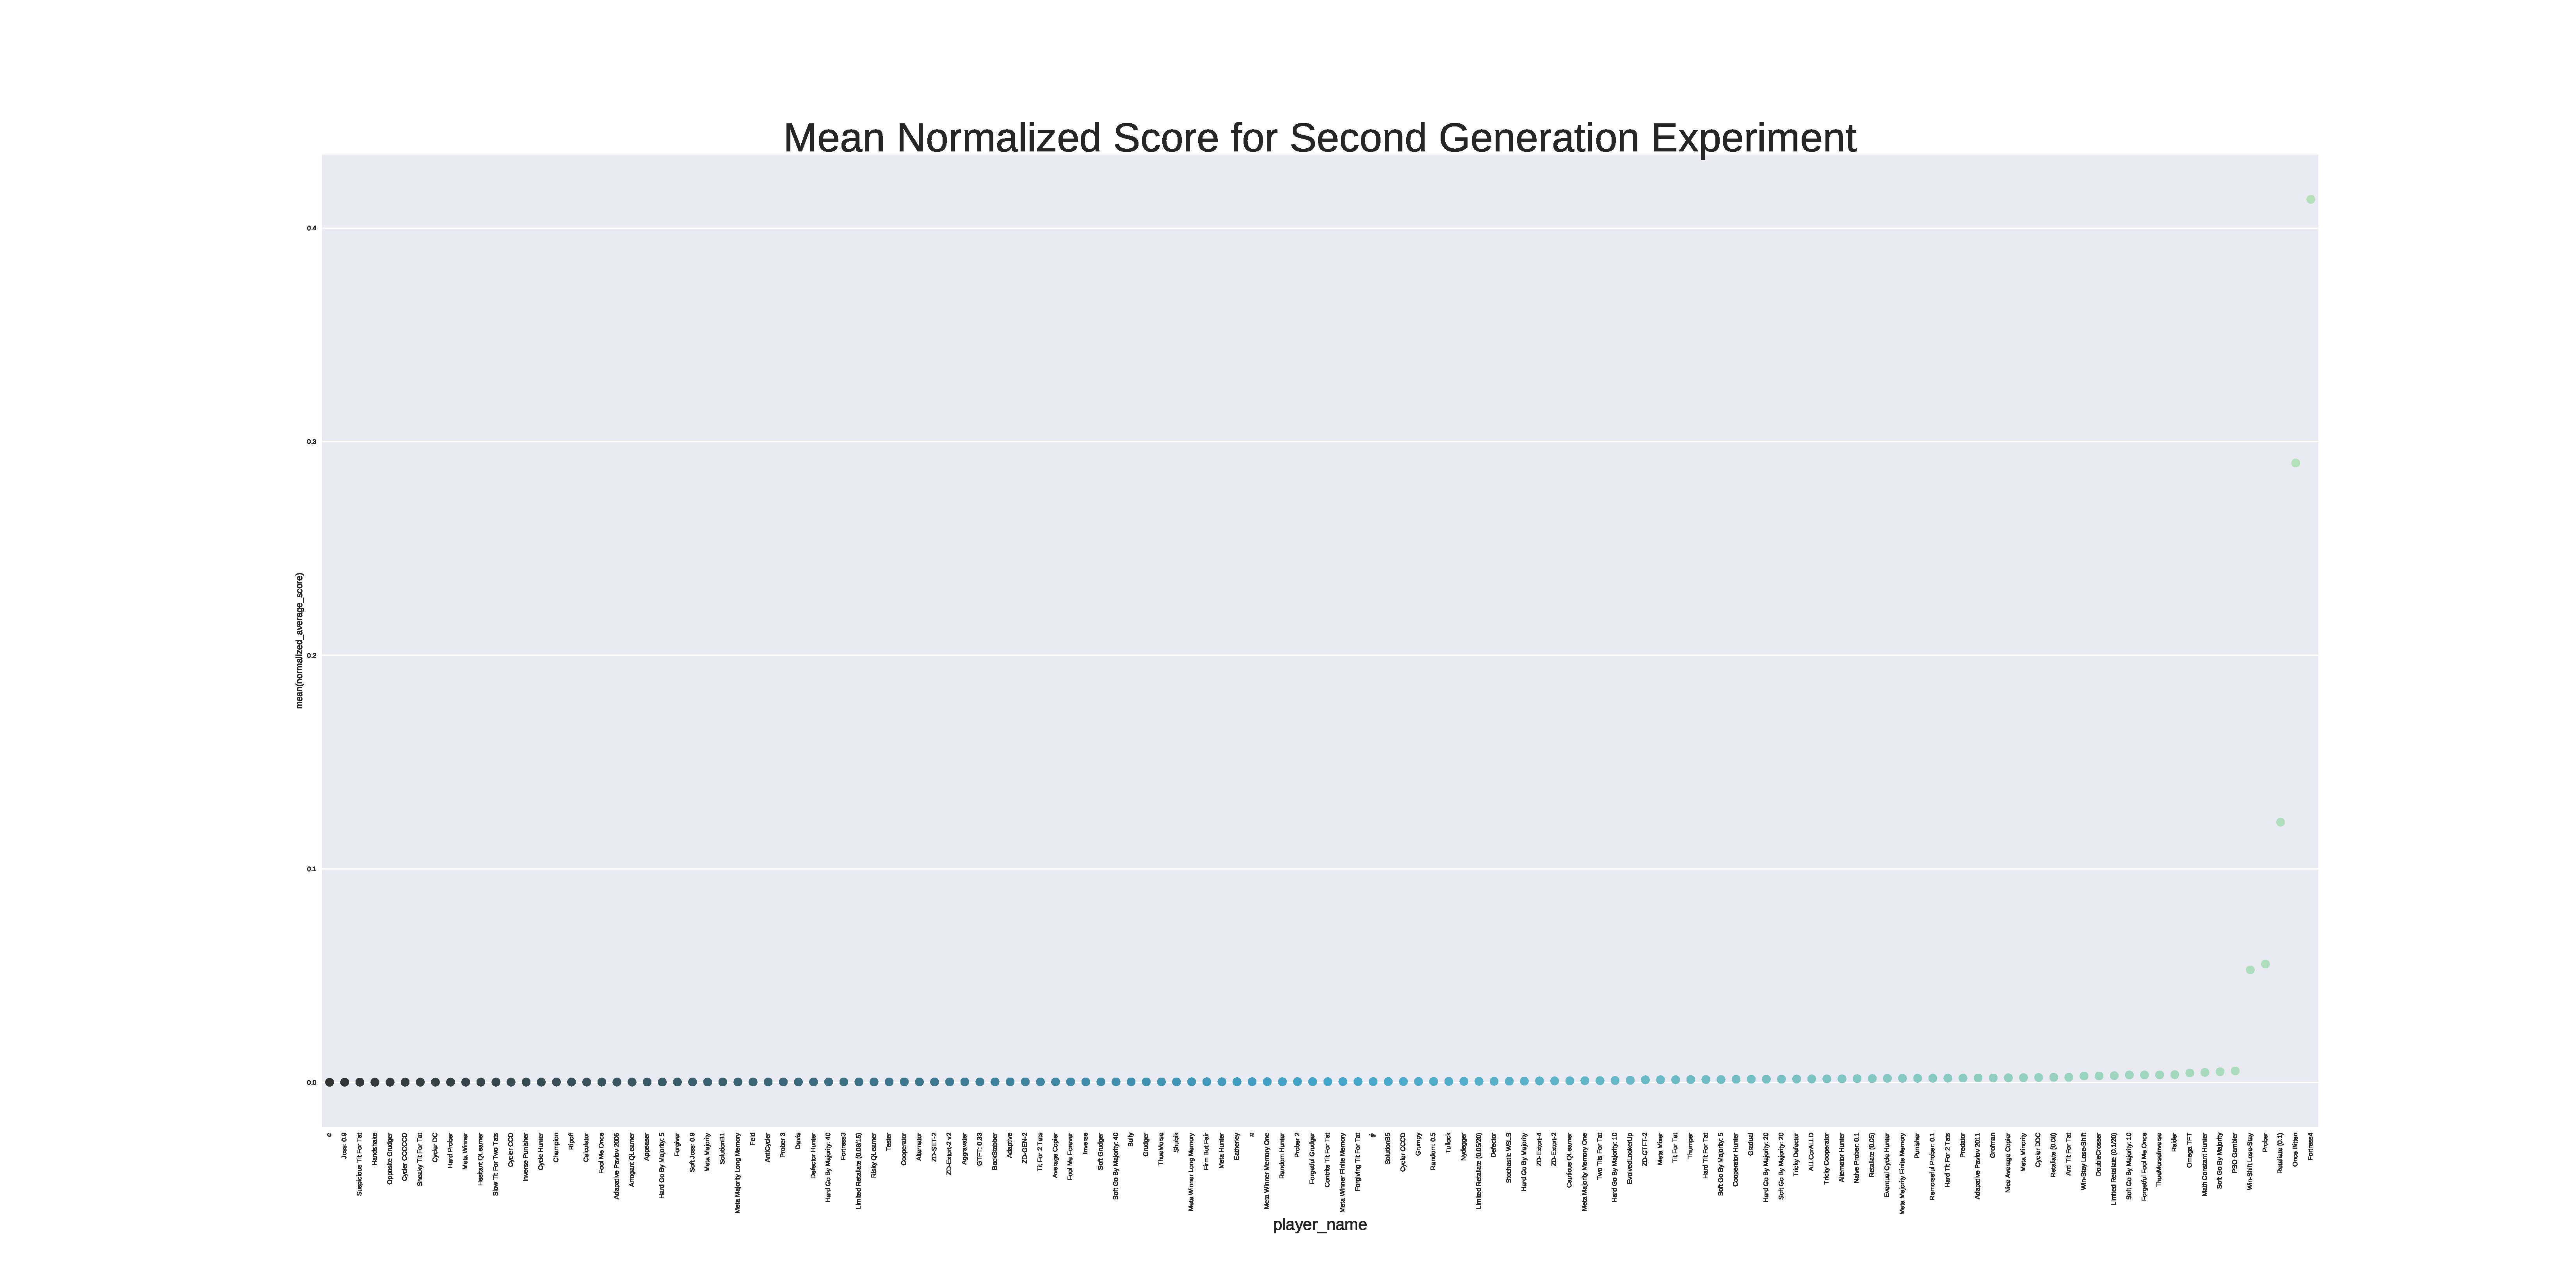
\includegraphics[width=1.2\linewidth,center]{chapter-four/score-ranking.pdf}
	\caption{Ranks based on normalized score}
	\label{fig:wining-second-gen}
\end{figure}

\subsection{Median Normalized Rank}

This part of the chapter, focuses on a new measure of performance. The
median normalized rank of the strategies. The normalized rank is computed
by dividing each rank of a strategy for a specific tournament by the corresponding
size of the tournament. The median rank is believed to be a more accurate
measure of performance, compared to winning ratio and normalized score.
As it will reveal strategies, that did not necessarily achieved the maximum wins,
but had an overall satisfying and smoothly performance throughout the experiment.

The median normalized score has been computed for each strategy and the ranks
are illustrated by the point plot in Figure~\ref{fig:ranking-second-gen}.~\footnote{A reminder,the
	lowest the rank the higher a strategy scored. 0 is the highest rank a strategy
can achieve in a tournament.} The strategies with the lowest median ranking are,
Meta Majority Finite Memory, Meta Minority and Limited Retaliate (0.1/20).
On the other hand, the highest ranked strategies are the following:

\begin{itemize}
	\item Fourth with a median ranking equal to 0.29, PSO Gambler
	\item Third with a median ranking equal to 0.27, Nydegger
	\item Second with a median ranking equal to 0.25, Cautious QLearner
	\item First with a median ranking equal to 0.23, Gradual
\end{itemize}

\begin{figure}[!hbtp]
	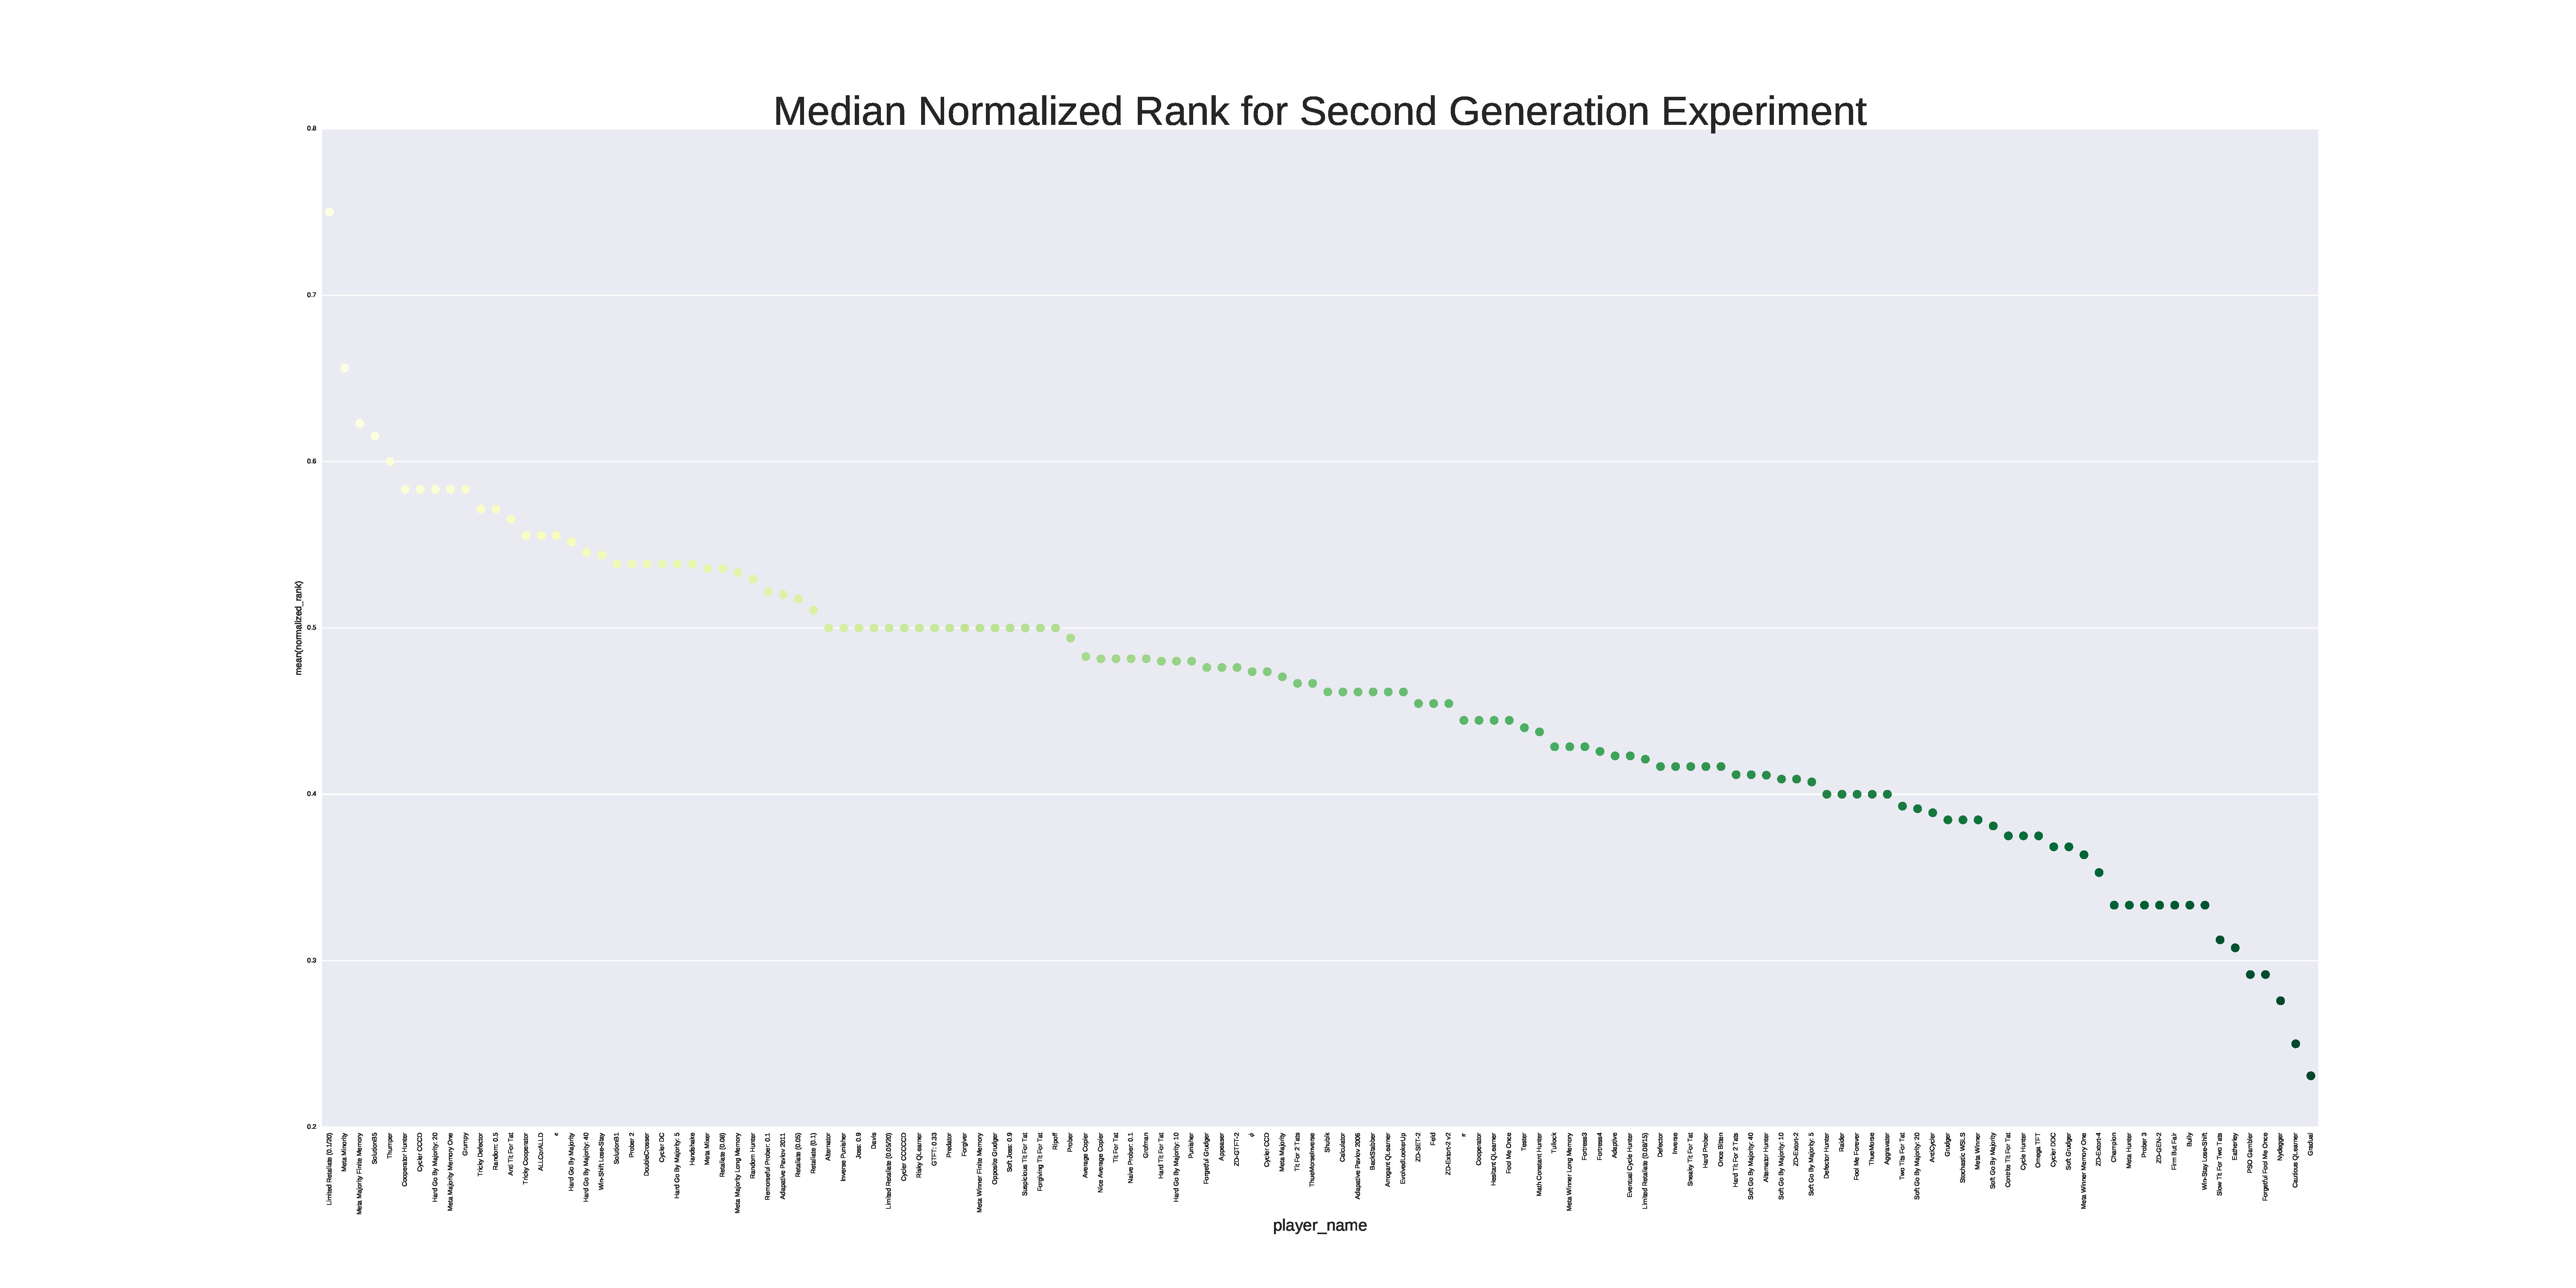
\includegraphics[width=1.2\linewidth,center]{chapter-four/median-ranking.pdf}
	\caption{Normalized Median Rank Complex Networks Experiments}
	\label{fig:ranking-second-gen}
\end{figure}

Both PSO Gambler and Gradual are well performed strategies in the Axlerod-Python
tournament. Furthermore, apart from PSO Gamber, which is a moderate cooperative
strategy, the rest are characterized as high cooperators. Further research on
the cooperation ratio will be executed in the following subsection.

To investigate the effect of networks topologies in the findings, a Kruskal Wallis test
has been executed. The existence of a statistically significant difference between
the normalized ranking and the clustered groups, as stated in ~\autoref{sub:classification} based on the
connectivity and clustering coefficients, is being tested. A non parametric test
is used, because ranks are not a normally distributed measure. For the Kruskal Wallis
test the scipy python library is being used once again.

The finding of the tests returned the following results. There is significant
difference on the normalized ranking between the clustered groups(\(p\)
value less than 0.05). Thus, depending on the topology the ranks differ.
Figure~\ref{fig:variation-clusters}, shows that there is a increasing trend.
Because the clusters seems to be affected more from the connectivity coefficients,
it could be assumed that as the connectivity increases the rank does as well.

\begin{figure}[!hbtp]
	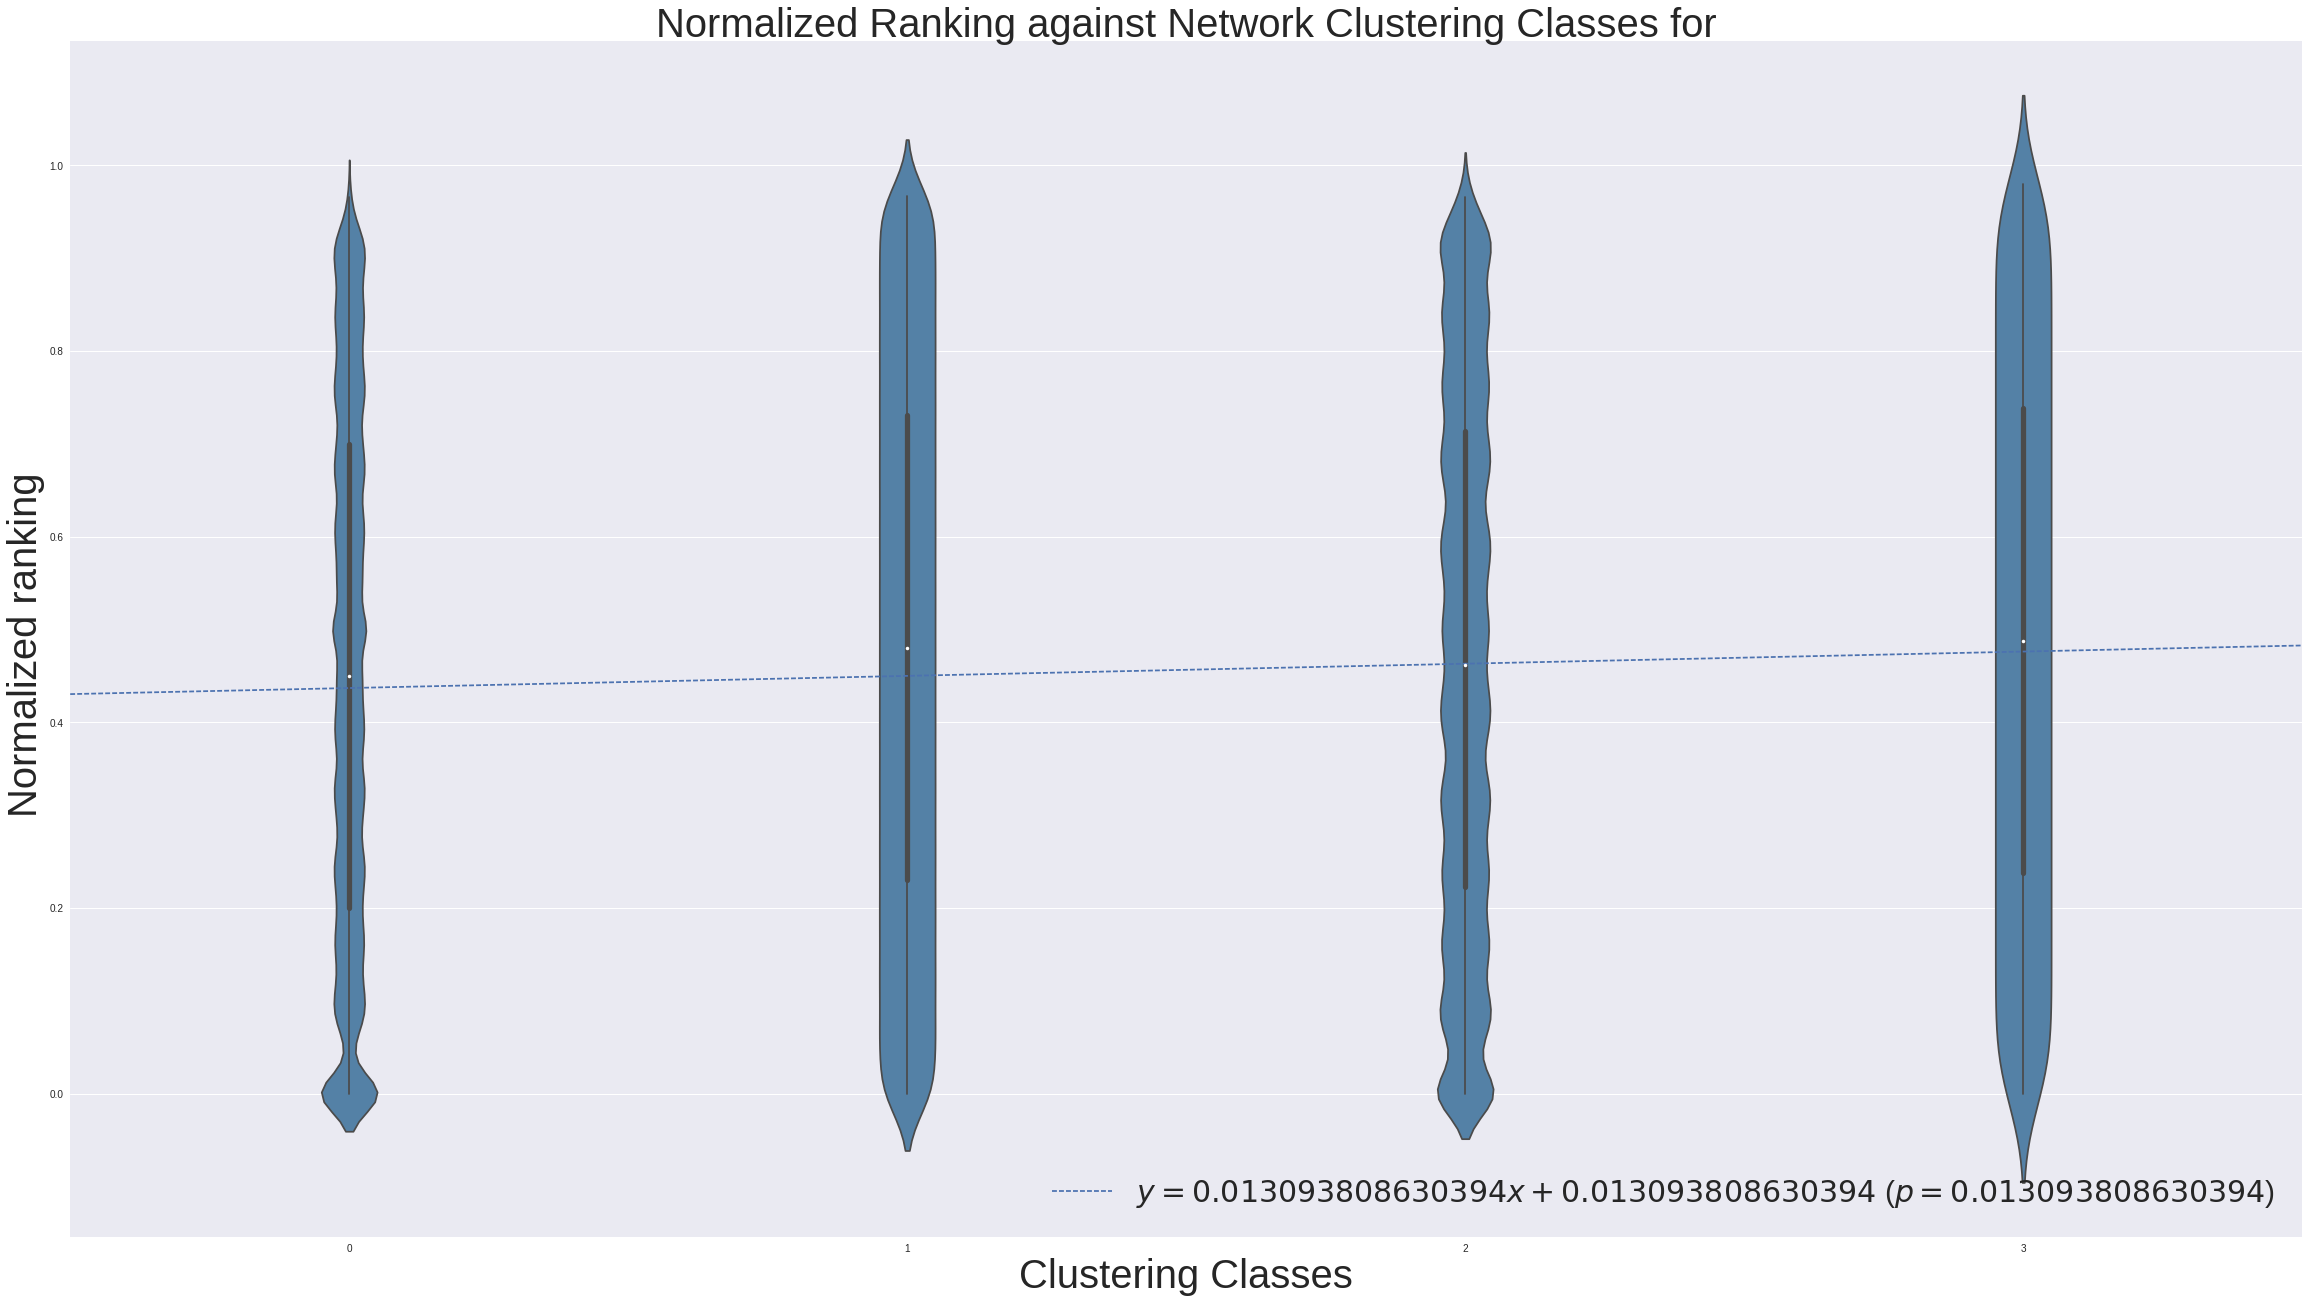
\includegraphics[width=1.2\linewidth,center]{chapter-four/normalized-rank-clusters.png}
	\caption{Violin Plot of Clusters against Median Normalized Ranking}
	\label{fig:variation-clusters}
\end{figure}

In this subsection, PSO Gamber, Nydegger, Cautious QLearner, Gradual, have been
defined as the best performing strategies based on the median ranking.
Furthermore, the difference in the strategies normalized ranks have been studied,
based on groups of network clustering and connectivity. The results indicated,
statistically significant difference. The effects of clustering and connectivity
coefficients will be analyzed in the following subsection by building regression
models.

\subsection{Regression}
This subsection concentrates, into build a regression model, for predicting
the normalized ranking of a strategy. This has been done, by identifying any
correlation between the topology measures and the participations of the strategy.
Initially, an analysis was performed for the entire data set, using the following
model.

\begin{align}
	\mathrm{normalised.ranking}_{t} = \alpha
	  & + \beta_{1}  \mathrm{average.neighborhood.score}_{t}          \\
	  & + \beta_{2}  \mathrm{normalized.average.score}_{t}            \\
	  & + \beta_{3}  \mathrm{cooperating.ratio}_{t}                   \\
	  & + \beta_{4}  \mathrm{connectivity}_{t}                        \\
	  & + \beta_{5}  \mathrm{clustering}_{t}                          \\
	  & + \beta_{6}  \mathrm{neighborhood.size}_{t}                   \\
	  & = \beta_{7}  \mathrm{tournament.size}_{t}                     \\
	  & + \beta_{8}  \mathrm{number.of.participations}_{t} + \epsilon
\end{align}

The result of the model are shown in Table~\ref{regression-complex-networks}.
All the predictors, expect clustering and neighborhood size, are significant.
Due their \(p\) value being less than 0.05.
Apart from normalized average score, connectivity and cooperating ratio, all
variables have a positive correlation with the normalized ranking. Because the
objective function, is to minimize the ranking, normalized average score,
connectivity and cooperating ratio are the only predictors affecting the performance
of a strategy positively. The model itself has a \(R\) squared value of 0.006.

\begin{table}[!hbtp]
	\centering
	\begin{adjustbox}{width=0.7\textwidth}
		\small
		\begin{tabular}{llll}
			\toprule
			\multicolumn{4}{|c|}{\textbf{Regression Results}}         \\ \hline
			                           & coefficient & \(p\) value & \(R\)-squared \\ \hline
			Intercept                  & 0.3712      & 0.000       & 0.006     \\ \hline
			average.neighborhood.score & 0.0206      & 0.000       & -         \\ \hline
			normalized.average.score   & -0.6150     & 0.001       & -         \\ \hline
			clustering                 & 0.0033      & 0.033       & -         \\ \hline
			connectivity               & -0.0011     & 0.000       & -         \\ \hline
			cooperating.ratio          & -0.0403     & 0.000       & -         \\ \hline
			tournament.size            & 0.0033      & 0.000       & -         \\ \hline
			frequency                  & 1.35e-06    & 0.000       & -         \\ \hline
			neighborhood.size          & 0.0005      & 0.017       & -         \\ \bottomrule

		\end{tabular}
	\end{adjustbox}
	\caption{Regression results}
	\label{regression-complex-networks}
	explaingn
\end{table}

The ability of the model to predict each of the 132 strategies has also been
tested. The results of each regression model in detail can be found in the
Appendix~\ref{append:reg-results-strategies}.

The results of implementing the models for each of the top ranking and the worst
ranking strategies are being discussed. The individual results of the best
performed strategies are shown in Table~\ref{reg-for-top}. The findings summarized
are the following,

\begin{itemize}
	\item PSO Gambler's, performance was significantly affected only by the tournament size
	\item Nydegger's, performance was significantly affected by clustering of the network,
	      the tournament size and the average neighborhood score
	\item Cautious QLearner's, performance was significantly affected by the tournament size,
	      the average neighborhood score and the normalized average score
	\item Gradual's, performance can not be predicted by the model
\end{itemize}

Overall, for each strategy the model had an low value of \(R\), thus there models
can only explain a small amount of variation in the normalized score of the strategies.
\begin{table}[!hbtp]
	\centering
	\begin{adjustbox}{width=1\textwidth}
		\small
		\begin{tabular}{|l|l|l|l|l|l|l|l|l|l|l|l|l|}
			\toprule
			\multicolumn{13}{|c|}{\textbf{Regression Results}}                                                                       \\ \hline
			& \multicolumn{3}{l|}{PSO Gambler} & \multicolumn{3}{l|}{Nydegger} & \multicolumn{3}{l|}{Cautious QLearner} & \multicolumn{3}{l|}{Gradual} \\ \hline
			                           & coefficient  & \(p\) value & \(R\)-squared & coefficient & \(p\) value & \(R\)-squared & coefficient & \(p\) value & \(R\)-squared & coefficient     & \(p\) value & \(R\)-squared \\ \hline

			Intercept                  & 4.400080e-07 & 0.624059    & 0.070179      & 2.729e-09   & 0.269       & 0.042         & 1.508e-08   & 0.114       & 0.129         & 8.626e-08       & 0.058       & 0.020         \\ \hline
			average.neighborhood.score & -0.019826    & 0.863098    & -             & 0.0475      & 0.043       & -             & 0.1716      & 0.000       & -             & -0.0301         & 0.478       & -             \\ \hline
			normalized.average.score   & -28.609297   & 0.46898     & -             & 114.0857    & 0.163       & -             & -653.0862   & 0.000       & -             & 83.8451         & 0.339       & -             \\ \hline
			connectivity               & -0.007497    & 0.111566    & -             & -0.0019     & 0.316       & -             & 0.0043      & 0.110       & -             & 0.0006          & 0.838       & -             \\ \hline
			clustering                 & 0.104217     & 0.505338    & -             & -0.0749     & 0.004       & -             & -0.0594     & 0.059       & -             & -0.0108         & 0.785       & -             \\ \hline
			cooperating.ratio          & -0.081274    & 0.66987     & -             & 0.0456      & 0.331       & -             & 0.0673      & 0.497       & -             & -0.1310         & 0.082       & -             \\ \hline
			tournament.size            & 0.021194     & 0.000553    & -             & 0.0100      & 0.000       & -             & 0.0176      & 0.000       & -             & 0.0037          & 0.080       & -             \\ \hline
			frequency                  & 0.000268     & 0.624046    & -             & 4.884e-06   & 0.758       & -             & 3.942e-05   & 0.196       & -             & 0.0002          & 0.054       & -             \\ \hline
			neighborhood.size          & -0.003179    & 0.512211    & -             & 0.0004      & 0.844       & -             & -0.0066     & 0.033       & -             & 0.0005          & 0.894       & -             \\ \bottomrule

		\end{tabular}
	\end{adjustbox}
	\caption{Regression results for PSO Gambler, Nydegger, Cautious QLearner and Gradual}
	\label{reg-for-top}
\end{table}

Moreover, the results of the three worst ranking strategies are shown in Table~\ref{reg-for-bot}.
A summary of the results is as follows:
\begin{itemize}
	\item Meta Majority Finite Memory's performance was only significant affected by the tournament size
	\item Meta Minority's performance was only significant affected by the average neighborhood score
	      and the neighborhood size
	\item Limited Retaliate's (0.1/20) performance is significant affected by normalized average score,
	      cooperating ratio and  neighborhood size.
\end{itemize}

Similarly, each of the \(R\) square values is significant low. Thus, even if some
predictors were identified as statistically significant, due the low \(R\) square values
it is clear that the model can not predict the performance of either the top or low ranking strategies.

\begin{table}[!hbtp]
	\centering
	\begin{adjustbox}{width=0.9\textwidth}
		\small
		\begin{tabular}{|l|l|l|l|l|l|l|l|l|l|l|l|l|}
			\toprule
			\multicolumn{10}{|c|}{\textbf{Regression Results}}                                                                       \\ \hline
			& \multicolumn{3}{l|}{Meta Majority Finite Memory} & \multicolumn{3}{l|}{Meta Minority} & \multicolumn{3}{l|}{Limited Retaliate (0.1/20)}\\ \hline
			                           & coefficient  & \(p\) value & \(R\)-squared & coefficient   & \(p\) value & \(R\)-squared & coefficient & \(p\) value  & \(R\)-squared \\ \hline
			Intercept                  & 4.400080e-07 & 0.624059    & 0.070179      & -4.705709e-08 & 0.731064    & 0.037403      & 0.000002    & 2.461325e-18 & 0.103475      \\ \hline
			average.neighborhood.score & -0.019826    & 0.863098    & -             & 0.178246      & 0.001111    &               & -0.08878    & 0.19002      & -             \\ \hline
			normalized.average.score   & -28.609297   & 0.46898     & -             & 393.594243    & 0.074333    &               & -133.372492 & 0.000048     & -             \\ \hline
			connectivity               & -0.007497    & 0.111566    & -             & 0.002575      & 0.459493    &               & 0.009121    & 0.093335     & -             \\ \hline
			clustering                 & 0.104217     & 0.505338    & -             & 0.23341       & 0.029178    &               & -0.189418   & 0.109777     & -             \\ \hline
			cooperating.ratio          & -0.081274    & 0.66987     & -             & -0.631593     & 0.052838    &               & 0.346784    & 0.003463     & -             \\ \hline
			tournament.size            & 0.021194     & 0.000553    & -             & -0.002791     & 0.515109    &               & -0.03785    & 1.093118e-08 & -             \\ \hline
			frequency                  & 0.000268     & 0.624046    & -             & -0.000069     & 0.715793    &               & 0.002028    & 2.459952e-18 & -             \\ \hline
			neighborhood.size          & -0.003179    & 0.512211    & -             & -0.008742     & 0.014707    &               & 0.012772    & 0.019486     & -             \\ \bottomrule
		\end{tabular}
	\end{adjustbox}
	\caption{Regression results for ​Meta Majority Finite Memory, Meta Minority and Limited Retaliate (0.1/20)}
	\label{reg-for-bot}
\end{table}

Even so, the lowest ranked strategies have not been the strategies with the lowest
\(R\) square values. As it seems there have been other strategies to which their behavior
could not be predicted at all. These strategies were Davis, Soft Go By Majority: 10
and Contrite Tit For Tat. Their results after applying the regression model
can be seen in Table~\ref{reg-for-r-bot}.

\begin{table}[!hbtp]
	\centering
	\begin{adjustbox}{width=0.9\textwidth}
		\small
		\begin{tabular}{|l|l|l|l|l|l|l|l|l|l|l|l|l|}
			\toprule
			\multicolumn{10}{|c|}{\textbf{Regression Results}}                                                                       \\ \hline
			& \multicolumn{3}{l|}{Davis} & \multicolumn{3}{l|}{Soft Go By Majority: 10} & \multicolumn{3}{l|}{Contrite Tit For Tat}\\ \hline
			  & coefficient & \(p\) value & \(R\)-squared & coefficient & \(p\) value & \(R\)-squared & coefficient & \(p\) value & \(R\)-squared \\ \hline
			Intercept 								 &2.671044e-09  & 0.000355			& 0.002087	& 1.203656e-06	& 0.052384	& 0.003057	& -3.037859e-08 & 0.019441		 & 0.004457	\\ \hline
			average.neighborhood.score & 0.011477			& 0.210965			&	-					& -0.129346			& 0.272084 	& -					& 0.029967  		& 0.152437			& -         \\ \hline
			normalized.average.score	 & 8.706744			& 0.880304 			&	-					& 34.423987			& 0.836946 	& -					& 1364.800701 	& 0.005748			& -         \\ \hline
			connectivity							 & 0.000593			& 0.677547			&	-					& 0.005444			& 0.269910 	& -					& -0.000883			& 0.644392			& -         \\ \hline
			clustering  							 & 0.035832			& 0.005207			&	-					& -0.081300			& 0.606653	& -					& -0.030868 		& 0.117834			& -         \\ \hline
			cooperating.ratio					 & 0.007705			& 0.616883			&	-					& 0.030627 			& 0.944789 	& -					& -0.244267			& 0.017799			& -         \\ \hline
			tournament.size						 &-0.000044			& 0.948541			&	-					& -0.001665 		& 0.792195 	& -					& 0.004213 			& 0.000513			& -         \\ \hline
			frequency									 &0.000035			& 1.373152e-76	&	-					& 0.000919			& 5.214774e-02	& -			&  0.000002			& 8.786468e-01	& -         \\ \hline
			neighborhood.size			     &-0.001045			& 0.512251 			&	-					& -0.003463			& 0.487918			& -			& -0.000123 		& 0.954622	& -         		\\ \bottomrule
		\end{tabular}
	\end{adjustbox}
	\caption{Regression results for Davis, Soft Go By Majority: 10 and Contrite Tit For Tat}
	\label{reg-for-r-bot}
\end{table}

The only strategies that could be predicted by the model have been Fortress4 and
Once Bitten. For both strategies the model achieved a \(R\) square value of
0.80. Thus the model can explains 80 \% of the normalized rank variability for
each of the strategies. Results are given by Table~\ref{reg-for-r-top}.

\begin{table}[!hbtp]
	\centering
	\begin{adjustbox}{width=0.9\textwidth}
		\small
		\begin{tabular}{|l|l|l|l|l|l|l|l|l|l|l|l|l|}
			\toprule
			\multicolumn{7}{|c|}{\textbf{Regression Results}}                                                                       \\ \hline
			&	\multicolumn{3}{l|}{Fortress4} & \multicolumn{3}{l|}{Once Bitten}\\ \hline
			  											   & coefficient & \(p\) value & \(R\)-squared & coefficient & \(p\) value & \(R\)-squared \\ \hline
			Intercept 								 & 7.664265e-01	& 6.883006e-01	& 0.800519	& 2.478012e-01 & 1.947868e-01 & 0.849582	\\ \hline
			average.neighborhood.score & 4.524753			& 8.618145e-01	& -					& 3.584271		 & 2.754952e-01	& -         \\ \hline
			normalized.average.score	 & -61.647292		& 3.363273e-01	& -					&-62.682017 	 & 3.283353e-01	& -         \\ \hline
			connectivity							 & -0.264150		& 6.877932e-01	& -					&-0.044507 		 & 3.574439e-01	& -         \\ \hline
			clustering  							 & 0.766427			& 6.883006e-01	& -					& 0.247801 		 & 1.947868e-01	& -         \\ \hline
			cooperating.ratio					 & -67.421175		& 5.575154e-01	& -					&-20.229438		 & 7.362663e-02	& -         \\ \hline
			tournament.size						 & 0.502277			& 6.893652e-01	& -					&0.203294  		 & 1.573032e-01	& -         \\ \hline
			frequency									 & 4.598559			& 6.883006e-01	& -					&2.230211  		 & 1.947868e-01	& -         \\ \hline
			neighborhood.size			   	 & -0.264150			& 0.687793		& -					&-0.044507 		 & 0.357444	& -         		\\ \bottomrule

		\end{tabular}
	\end{adjustbox}
	\caption{Regression results for ​Fool Me Forever, Fortress4 and Once Bitten}
	\label{reg-for-r-top}
\end{table}

In this subsection, the performance of the strategies has been tried to be predicted
by a regression model. The results, for running this regression model to the
hole data set returned that cooperating ratio, connectivity and the normalized
average score were significant predictors. Furthermore, by analyzing each strategy
individual to test whether their behavior can be predicted, returned that this
is possible for only 2 of the 132 strategies. For the rest, their performance can not
be accurately predicted by the possible predictors given. In the next section,
a summary of the findings of this chapter have been stated.

\section{Summary}
In this chapter, experiments with more complex networks topologies have been
performed. Various networks have been considered: all with a varying topological
structure, obtained using methods to create random and small world networks.

The methods have been individual discussed and an overview of the data they
produced has been implemented. To be able to perform analysis on the data set
produced by using this methods, two classification have been conducted.
In this chapter, a new measure has been used, the normalized median rank.
The four top performed strategies of the complex networks experiment have
been named. PSO Gamblre, Nydegger, Cautious QLearner and Gradual.

An analysis of the normalized ranking was then conducted. The findings are the
following. Normalized ranking, for the top strategies have been significantly different
between groups of connectivity, clustering and cooperating. Also cooperating behavior, has been showed to
be affecting the performance. All three strategies have been characterized as highly
cooperators by the analysis in ~\ref{sub:four-classification}. Regression showed that,
predicting the performance of the strategies is possible of 2 of the 132 strategies.
Even so, this could be further investigated.

In conclusion, further research with more data and different random topology
is needed. Thought connectivity and cooperating ratio seems to have played a role,
there is not enough validation in the results. The topology does in did affect
the strategies, but a strategy that could outperform any topology has now been
found yet. Whether a strategy like this exist or not in the Axlerod Python Library
is not sure. Thus, in the following chapter a strategy will be trained.
% miyagi

\chapter{Training Strategy using Evolutionary Algorithm}
\section{Introduction}
\label{sub:five-intro}
This chapter covers an overview on the contribution of Professor M Jones
in the Axelrod-Python library. Following the presentation of Axelrod-Python
library at PyConUk 2015~\url{http://2016.pyconuk.org/}, he became a member of
the Axelrod-Python team and contributed to the library a new strategy, the
EvolvedLookerUp, which is currently ranked second in the Axlerod-Python tournament.
EvolvedLookerUp is a LookerUp strategy that uses a lookup table generated using an
evolutionary algorithm. The structure of the strategy and the evolution algorithm
will be covered in the following sections.

Furthermore, the method developed by M Jones to train the EvolvedLookerUp
will be redeveloped and used. Making it possible to train a new strategy
by competing against random opponents into various spatial tournaments.

%A brief introduction to the genetic algorithm will also be covered.

\section{The Lookup Evolve Algorithm}
\label{sub:lookup-evolve-algorithm}
As stated in ~\autoref{sub:five-intro}, the LookerUp strategies uses a lookup to
determine the strategy's next move. In this section, the lookup table, as well as
the LookerUp strategies are explained. Additionally, the mechanism used for the
maximization of these strategies performance will be discussed.

\subsection{The Lookup Table}
The strategies of the Axelrod-Python library have access to their own history,
through the \texttt{self.history} variable and the opponent's history though
\texttt{opponent.history} variable. Many strategies choose their actions based
on what happened on previous turns\footnote{Only two actions are possible in the
IPD; to either Cooperate(C) or to Defect(D).}. This rule, of determining once actions
based on a history can be think of as a lookup table.
In Jones work three different histories are taken into account:

\begin{itemize}
  \item the opponents two starting actions
  \item the opponent's two recent actions
  \item and the recent actions of the strategy.
\end{itemize}

Using Python's dictionaries the histories can be considered as keys and
the action as the values. Thus, the keys are a 3-tuples consisting of the opponent's
starting actions, the opponent's recent actions, and the strategy's recent actions.
The lookup table in total contains 64 different keys and a key/value pairs example
is illustrated in Listing~\ref{lst:lookup-table}.

\begin{listing}[H]
\usemintedstyle{tango}
\begin{minted}
[
frame=lines,
framesep=2mm,
baselinestretch=1.2,
bgcolor=LightGray,
fontsize=\footnotesize,
linenos
]
{python}
lookup_table = {
    ...
    ('CC', 'CC', 'DD') : 'D',
    ('DD', 'CC', 'DD') : 'C',
    ...
}
\end{minted}
\caption{Example of lookup table}
\label{lst:lookup-table}
\end{listing}

The lookup table corresponds to a guideline which the strategy determines it's following action.
A class for generating a strategy object, which  will take into account a lookup tables,
for playing the IPD game is described in the following subsection.

\subsection{The LookerUp class}

The LookerUp class, is generating a object for a given lookup table.
The source code of the class, as written by M Jones, is illustrated in the
Listing~\ref{lst:lookerup}. As shown, the strategy taken as an argument
a lookup table and therefore plays by following these regulations:
\begin{itemize}
  \item If history is smaller than 2, then  always cooperate
  \item if history is greater than 2, create key
  \item check lookup table for corresponding key and value
  \item return value as action
\end{itemize}

\begin{listing}[H]
\usemintedstyle{tango}
\begin{minted}
[
frame=lines,
framesep=2mm,
baselinestretch=1.2,
bgcolor=LightBlue,
fontsize=\footnotesize,
linenos
]
{python}
class LookerUp(Player):

    def __init__(self, lookup_table):
        self.lookup_table = lookup_table


    def strategy(self, opponent):
        # If there isn't enough history to lookup an action, cooperate.
        if len(self.history) < 2:
            return C

        # Get my own last two actions
        my_history = ''.join(self.history[-2:])

        # Do the same for the opponent.
        opponent_history = ''.join(opponent.history[-2:])

        # Get the opponents first two actions.
        opponent_start = ''.join(opponent.history[:2])

        # Put these three strings together in a tuple.
        key = (opponent_start, my_history, opponent_history)

        # Look up the action associated with that tuple in the lookup table.
        action = self.lookup_table[key]

        return action
\end{minted}
\caption{The LookerUp class source code}
\label{lst:lookerup}
\end{listing}

The class is used to test the performance of the table. EvolverLookerup, is a
later version of LookerUp, the difference is that EvolverLookerUp uses a satisfactory
table, crafted by using an evolutionary algorithm. The process will be described
in the following subsection.

\subsection{Evolutionary Algorithm}
\label{sub:evolutionary-algorithm}
The performance of a lookup table is measured as the average score the lookup
strategy achieves in a round robin tournament against all strategies in the
Axelrod-Python library. Though various optimization processes could have been
used for the maximization of the objective function,
the genetic algorithm was preferred. Genetic algorithm, is a commonly used adaptive
algorithm for solving practical problems. An introduction in the genetic algorithm
has been covered by M Mitchell~\cite{Mitchell1998}, and along various applications~\cite{Chang1994}
it has been used in the field of Game Theory as well~\cite{Ismail2007}.

The lookerup evolve algorithm, which is the algorithm that tries to maximize
the performance using the genetic algorithm is described by the flow chart in
Figure~\ref{fig:flookerup-evolve-flow}. The algorithm starts off by creating
\(n\) number of random tables. These tables are then passed in genetic algorithm
as the current tables.
Once the genetic algorithm kicks off children are reproduced for every single pair
of parents. The reproduction process included random crossovers as well as a
mutation rate \(u\). Subsequently, the population is defined as the joint of
parents and children.

Each member of the population has to go through the scoring process. A different
object of the LookerUp strategy is created for each of the lookup tables that
exist in the population, and each object participates to a round robin tournament.
Thereupon, the population is being sorted based on the average score per turn.
Only the top \(b\) individuals are then selected to continue to the next generation.
This is repeated until the number of generations reach the upper bound \(g\).

The default values of the parameters in the lookerup evolve algorithm are as
follow:
\begin{itemize}
  \item \(n\) default value is equal to 5
  \item \(u\) default value is equal to 0.1
  \item \(b\) default value is equal to 10
  \item \(g\) default value is equal to 100
\end{itemize}

\begin{figure}[!hbtp]
		\tikzstyle{startstop} = [rectangle, rounded corners, minimum width=2cm, minimum height=1cm,text centered, draw=black, fill=black!40]
\tikzstyle{process} = [rectangle, minimum width=0.5cm, minimum height=1cm, text centered, draw=black,text width=13cm]
\tikzstyle{decision} = [diamond, minimum width=0.5cm,text width=3cm, minimum height=1cm, text centered, draw=black, fill=green!30]
\tikzstyle{arrow} = [thick,->,>=stealth]

\begin{center}
\begin{tikzpicture}[scale=3, node distance=1.5cm, auto, execute at begin node={\begin{varwidth}{40em}},
                    execute at end node={\end{varwidth}}]

% start flow chart
\node (start) [startstop] {Start};
% get first tables
\node (in1) [process, below of=start , fill=black!5] {\small \textbf{Current Tables} $\leftarrow$ \(n\) Random Generated Lookup Tables};
% start genetic
\node (pro1) [process, below of=in1, fill=blue!50] {\small \textbf{Start Genetic Algorithm}};
% parents
\node (pro2) [process, below of=pro1, fill=black!5] {\small \textbf{Parents} $\leftarrow$ Current Tables + \(n\) Random Generated Lookup Tables};
% kids
\node (in2) [process, below of=pro2, fill=black!5] {\small \textbf{Children} $\leftarrow$ all possible combinations of Parents};
%population
\node (pro3) [process, below of=in2, fill=black!5] {\small \textbf{Population} $\leftarrow$ Parents + Children};
%score them
\node (pro4) [process, below of=pro3, fill=blue!50] {\small \textbf{Score Population}};
%score them details
\node (pro5) [process, below of=pro4, fill=black!5] {\small LookerUp (for each lookup table) plays in a round robin tournament};
%ranked population
\node (in3) [process, below of=pro5, fill=blue!50] {\small \textbf{Ranked Population, based on average score}};
%keep rank
\node(pro6) [process, below of=in3, fill=black!5] {\small \textbf{Current Tables} $\leftarrow$ \(b\) number of individuals};
%check number of generation
\node (dec1) [decision, below of=pro6, yshift=-1.5cm] {\small Generations $\leqslant$ \(g\)};
%stop
\node (stop) [startstop, below of=dec1, yshift=-1.5cm] {Stop};
% LINES
\draw [arrow] (start) -- (in1);
\draw [arrow] (in1) -- (pro1);
\draw [arrow] (pro1) -- (pro2);
\draw [arrow] (pro2) -- (in2);
\draw [arrow] (in2) -- (pro3);
\draw [arrow] (pro3) -- (pro4);
\draw [arrow] (pro4) -- (pro5);
\draw [arrow] (pro5) -- (in3);
\draw [arrow] (in3) -- (pro6);
\draw [arrow] (pro6) -- (dec1);
\draw [arrow] (dec1) -|([xshift=-0.25cm]pro2.south west)|- node[anchor=east] {yes}(pro2);
\draw [arrow] (dec1) -- node[anchor=east] {no} (stop);
\end{tikzpicture}
\end{center}

		\caption{Lookerup Evolve Algorithm Flow Chart}
  \label{fig:flookerup-evolve-flow}
\end{figure}

In this section an overview of M Jones works was implemented. The full version
of the LookUpEvolver, his implementation of the genetic algorithm and the lookerup evolve
algorithm can be found here:\url{https://github.com/mojones/axelrod-evolver}.
In the upcoming section how the lookerup evolve algorithm was altered and used
for the spatial tournaments is being discussed.

\section{The Spatial Lookup Evolve Algorithm}

Inspired by the work done by M Jones, as was described in ~\autoref{sub:lookup-evolve-algorithm},
the lookup evolve algorithm will be used to train a new strategy. The goal is to
train a strategy, which will have an overall 'good' performance for any given
spatial tournament.

Large parts of the lookup evolve algorithm code that have already written
can be used. The main difference in this new spatial algorithm is the objective
function of the genetic algorithm.
\subsection{Objective Function}

In the approach of the spatial lookup evolve algorithm, one of the main differences
occurs in the objective function in the scoring process. Instead of the average
score in a round robin tournament, the median normalizes rank, as introduced
in ~\autoref{chap:Four}, for a spatial tournament is taken into account.

Using a similar approach to the one described in ~\autoref{chap:Four}, the objective
function will be the median rank a strategy achieved, after participating in \(p\)
random spatial tournaments of random different topologies. The tournament sizes
as well as the players participating in these tournaments are completely random.
The topologies can be that of a Watts Strogatz, a Erd\"{o}s
R\'{e}nyi or a complete graph. In Figure~\ref{fig:objective}, a flow chart
illustrates the idea of how this was implemented. Before and after the scoring
process the nodes are the same as have been seen in Figure~\ref{fig:flookerup-evolve-flow}.

\begin{figure}[!hbtp]
		\tikzstyle{process} = [rectangle, minimum width=0.5cm, minimum height=1cm, text centered, draw=black,text width=4.5cm]
\tikzstyle{decision} = [diamond, minimum width=0.5cm,text width=3cm, minimum height=1cm, text centered, draw=black, fill=green!30]
\tikzstyle{arrow} = [thick,->,>=stealth]

\begin{center}
\begin{tikzpicture}[scale=2, node distance=1.5cm, auto, execute at begin node={\begin{varwidth}{40em}},
                    execute at end node={\end{varwidth}}]

\node (before) [process] { ..... };
\node (pro4) [process, below of=before, fill=blue!80] {\small \textbf{Score Population}};

\node (sample) [process, below of=pro4] {\small Sample Players};

\node (decision) [decision, below of=pro4, yshift=-2.5cm] {\small Random Integer \(t\)};

\node (small) [process, below left=of decision, yshift=-0.4cm] {\small Watts Strogatz};

\node (random) [process, below of= decision, yshift=-2.5cm] {\small Erd\"{o}s R\'{e}nyi};

\node (complete) [process, below right=of decision, yshift=-0.4cm] {\small Complete};

\node (ranks1) [process, below of=random, yshift=-1.5cm] {\small Single Tournament Ranks};

\node (ranks2) [process, below of=ranks1, yshift=-1.5cm] {\small Median Normalized Ranks};

\node (after) [process, below of=ranks2] { ..... };
%Lines
\draw [arrow] (before) -- (pro4);
\draw [arrow] (pro4) -- (sample);
\draw [arrow] (sample) -- (decision);
\draw [arrow] (decision) -- node[anchor=west] {\(t\) = 0} (small);
\draw [arrow] (decision) -- node[anchor=west] {\(t\) = 1} (complete);
\draw [arrow] (decision) -- node[anchor=west] {\(t\) = 2} (random);
\draw [arrow] (small) -- (ranks1);
\draw [arrow] (random) -- (ranks1);
\draw [arrow] (complete) -- (ranks1);
\draw [arrow] (ranks1) -|([xshift=-0.25cm]pro2.south west)|- node[anchor=south] {repetitions $< =$ \(p\)} (sample);
\draw [arrow] (ranks1) -- node[anchor=west] {repetitions $>$ \(p\)} (ranks2);
\draw [arrow] (ranks2) -- (after);
\end{tikzpicture}
\end{center}

		\caption{Scoring Process for Spatial Lookup Evolve Algorithm}
  \label{fig:objective}
\end{figure}


Furthermore, for every given generation the current tables are being re scored.
Due the randomness that the scoring process includes and the fact that some
of the Axelrod-Python strategies are sophisticated, different scores for the
same lookup tables could occurs. Thus, the objective functions stops being
deterministic.

In addition, two different cases will be studied based on the strategies list.

\subsubsection{Non Deterministic}

The difference in these two cases occurs in the population of the strategies.
More specifically, for the non deterministic case
the population of strategies, from where the sample for participants for
the spatial games is being subtract, contains all 132 strategies of the
Axlerod-Python. The sample for each repetition \(p\) is randomly picked. For the
non deterministic case two sample sizes have been used. One from
15 to 50 players and the other one from 5 to 15 strategies.

\subsubsection{Deterministic}

For the deterministic case the population will contain only
the deterministic strategies of the Axelrod-Python library. The library provides
easy access to them and they have been identified as the following ten strategies:
\begin{itemize}
   \item Alternator
   \item Anti Tit For Tat
   \item Bully
   \item Cooperator
   \item Cycler DC
   \item Defector
   \item Suspicious Tit For Tat
   \item Tit For Tat
   \item Win-Shift Lose-Stay
   \item Win-Stay Lose-Shift
\end{itemize}

Thus the sample size this time will range between 5 to 10. Both of these
objectives are used for individual runs of the spatial lookup evolve algorithm.

\subsection{Parameters}

One can notice by the default values of the evolutionary algorithm parameters,
described in \autoref{sub:evolutionary-algorithm}, in each generation
144 lookup tables needed to be scored. Considering that each lookup table needs
to participate in \(p\) different spatial tournaments the time to implement
each generation is growing massively. The spatial lookup evolve algorithm
has been compiled in Raven, even so it still required a lot of time. Due to time
constraints of this dissertation these values had to altered. The new values
that have been used, alongside the values of the new parameters introduced
by the spatial version of the algorithm are listed here:
\begin{itemize}
    \item \(n\) default value is equal to 2
    \item \(u\) default value is equal to 0.1
    \item \(b\) default value is equal to 2
    \item \(g\) default value is equal to 5000
\end{itemize}

By setting \(n\) to 2 and by keeping only the 2 top of each generations only
20 lookup tables are being scored for each generation. Furthermore, the generations
have been set to 5000 though the results obtained and introduced in the following
subsection have been from earlier generations. The time limit for each algorithm
was set at 70 hours. The entire spatial scoring structure that
has been explained throughly during this subsection is illustrated in Figure~\ref{fig:spatial-evolve}.
Moreover, the source code for implementing the spatial version of the algorithm
are found here: \url{https://github.com/Nikoleta-v3/axelrod-evolver/tree/general-spatial}.

\begin{figure}[H]
		\tikzstyle{process} = [rectangle, minimum width=0.5cm, minimum height=1cm, text centered, draw=black,text width=4.5cm]
\tikzstyle{decision} = [diamond, minimum width=0.5cm,text width=3cm, minimum height=1cm, text centered, draw=black, fill=green!30]
\tikzstyle{arrow} = [thick,->,>=stealth]

\begin{center}
\begin{tikzpicture}[scale=3, node distance=1.5cm, auto, execute at begin node={\begin{varwidth}{40em}},
                    execute at end node={\end{varwidth}}]


\node (before) [process] { ..... };

%scoring process begins
\node (pro4) [process, below of=before, fill=blue!80] {\small \textbf{Score Population}};

%choose strategies population
\node (players) [decision, below of=pro4, yshift=-2cm] {\small Population \\ Strategies};
% two options
\node (list1) [process, below left=of players] {\small Deterministic Strategies};
\node (list2) [process, below right=of players]  {\small All Strategies};
% both go through sampling with different bounds
\node (sample) [process, below of=players, yshift=-3.5cm] {\small Sample Players};

\node (decision) [decision, below of=pro4, yshift=-10cm] {\small Random Integer \(t\)};

\node (small) [process, below left=of decision, yshift=-0.4cm] {\small Watts Strogatz};

\node (random) [process, below of= decision, yshift=-2.5cm] {\small Erd\"{o}s R\'{e}nyi};

\node (complete) [process, below right=of decision, yshift=-0.4cm] {\small Complete};

\node (ranks1) [process, below of=random, yshift=-1.5cm] {\small Single Tournament Ranks};

\node (ranks2) [process, below of=ranks1, yshift=-1.5cm] {\small Median Normalized Ranks};

\node (after) [process, below of=ranks2] { ..... };

%Lines
\draw [arrow] (before) -- (pro4);
\draw [arrow] (pro4) -- (players);
\draw [arrow] (players) -- (list1);
\draw [arrow] (players) -- (list2);
\draw [arrow] (list1) -- (sample);
\draw [arrow] (list2) -- (sample);
\draw [arrow] (sample) -- (decision);
\draw [arrow] (decision) -- node[anchor=west] {\(t\) = 0} (small);
\draw [arrow] (decision) -- node[anchor=west] {\(t\) = 1} (complete);
\draw [arrow] (decision) -- node[anchor=west] {\(t\) = 2} (random);
\draw [arrow] (small) -- (ranks1);
\draw [arrow] (random) -- (ranks1);
\draw [arrow] (complete) -- (ranks1);
\draw [arrow] (ranks1) -|([xshift=-1.5cm]sample.south west)|- node[anchor=south] {repetitions $<$ \(p\)} (sample);
\draw [arrow] (ranks1) -- node[anchor=west] {repetitions $<=$ \(p\)} (ranks2);
\draw [arrow] (ranks2) -- (after);
\end{tikzpicture}
\end{center}

		\caption{Complete Scoring Process for Spatial Lookup Evolve Algorithm}
  \label{fig:spatial-evolve}
\end{figure}

\section{Results}
In this sections the results of the spatial lookup evolve algorithm are briefly
presented. The results are divided into three categories based on the strategies
population and on the sample size. For each, the keys of the lookup table,
the lowest median normalized ranks and the generation it was achieved are given
in Table~\ref{results-genet}.

For the deterministic case the best strategy, with a score of 0.77 median normalized
rank, was achieved at the 319\nth generation. For the same generation the mean score
has been 0.57 with a standard deviation of 0.20. For the non deterministic case
and a sample size ranging from 5 to 15 the best lookup table has been achieved at
the 201\st generation. The best score was estimated at 0.769, with a mean population
of 0.36 and a standard deviation of 0.23. Finally, for the non deterministic with
a range of sample size between 15 and 50, the lowest median rank has been 0.68.
Thus, for a non deterministic case the specific lookup table generates
the best performed strategy so far.

\begin{table}[H]
\centering
\begin{adjustbox}{width=0.9\textwidth}
\small
\begin{tabular}{|l|l|l|l|}
\hline
\multicolumn{4}{|c|}{Results}                                                                                                                                                                                              \\ \hline
                                       & lookup values      & generation                                                                                         & score                                                   \\ \hline
  Deterministic                         & \begin{tabular}[c]{@{}l@{}}DDDDCDDDDCDCDCDDDCDCCDDCDDCCCDDC\\ CDCDCDCCDDCCCCDCDCCCCCCCDDCCDCCD\end{tabular} & 319  & 0.777778                                                     \\ \hline
  \begin{tabular}[c]{@{}l@{}}Non-deterministic\\ sample size(5-15)\end{tabular} & \begin{tabular}[c]{@{}l@{}}CDDCCDDDCDCDCDDDCDCDCCCCDCDDDCCC\\ DCDDDCDCDDCCDCDCCCDDCDDCCCDCCDDC\end{tabular} & 201 & 0.769231               \\ \hline
  \begin{tabular}[c]{@{}l@{}}Non-deterministic\\ sample size(15-50)\end{tabular}& \begin{tabular}[c]{@{}l@{}}DDDCCDDCCCCCDCCDDDCCCCCDDCCDDCDCC\\ CDDCDCDCDDCCCDCCCDCCCDDCDDDDDCD\end{tabular} & 148 & 0.6875                  \\ \hline
\end{tabular}
\end{adjustbox}
\caption{Results for Spatial Lookup Evolve Algorithm for Median Normalized Rank}
\label{results-genet}
\end{table}

For comparison reasons an extra algorithm has been performed. This time the
objective function has been measured as the minimum normalized score and was carried
out for only the non deterministic case.The results
that were generated from this run are given by the Table~\ref{results-min-geten}.
The overall results have been lower than before. The finest score has been achieved for
a sample size of 15 to 50 and returned an minimum normalized score of 0.478.

\begin{table}[H]
\centering
\begin{adjustbox}{width=0.8\textwidth}
\small
\begin{tabular}{|l|l|l|l|}
\hline
\multicolumn{4}{|c|}{Results}                                                                                                                                                                                             \\ \hline
                                     & lookup values  & generation   & score                                                                                                                                              \\ \hline
\begin{tabular}[c]{@{}l@{}}Non-deterministic\\ sample size(5-15)\end{tabular}   & \begin{tabular}[c]{@{}l@{}}DDDDDCCDCDCDDCCDCCDDCCCDDCDCDCDC\\ CCCCCCDCDCDDDDCCDCDCDDDDDCDDDDCD\end{tabular} & 47 & 0.692308                  \\ \hline
                                     & \begin{tabular}[c]{@{}l@{}}CCDCDCDDDCCDDCDCDCDDCCDCDDCDDDCD\\ CDCCDCCDDDDDCCCDCCDDDCDCDDDCCCDD\end{tabular}  & 13 & 0.692308                                                             \\ \hline
                                     & \begin{tabular}[c]{@{}l@{}}DCCCDDCCCDDCDDDDDDCDDCCDCCDDCDDD\\ DDDDCDDDDCCDDDDCCDCCCDDDCCCCCCCC\end{tabular}  & 8 & 0.692308                                                             \\ \hline
\begin{tabular}[c]{@{}l@{}}Non-deterministic\\ sample size(15-50)\end{tabular}& \begin{tabular}[c]{@{}l@{}}CDCCDDCDDDCCCDDDDCDCDCCDDCDCCDDD\\ DCDCCDCCCDDDCDDCDCDCDDCCCCCCDDDC\end{tabular} & 49 & 0.478261                     \\ \hline
\end{tabular}
\end{adjustbox}
\caption{Results for Spatial Lookup Evolve Algorithm for Minimum Normalized Rank}
\label{results-min-geten}
\end{table}

In this section the lookup tables that have been produced by the spatial lookup
evolve algorithm from each case that has been implemented were presented and discussed.
The finest lookup table for measuring the median normalized rank has been estimated
at 0.68. Furthermore, a new case of objective function has also been implemented
for comparison reasons. Additionally, in the following section the algorithm has
been perform for each of the networks individually.

\section{Further Results}

In this section some additional results of the spatial lookup evolve algorithm
are discussed. In the previous section the networks used in the scoring process
have been randomly picked between small world, random and complete networks.
In this section the algorithm has been implemented each of network and their
individual results are studied. This was implemented mainly for further results and
a possible identification of a well perform strategy for an individual topology.
Table~\ref{deter-indiv} and Table~\ref{no-deter-indiv} summarize the results.

For the deterministic case where the topology of the spatial tournaments has been
a Watts Strogatz networks, the first rate lookup table achieved a median normalized
score of 0, in the 635\nth generation. Moreover, for the Erd\"\{o\}sR\'\{e\}nyi
topology the finest lookup table has a score of 0.5 in the 1399\nth generation, similar
to the complete on where the lowest rank achieved has been 0.555556.

\begin{table}[H]
\centering
\begin{adjustbox}{width=0.8\textwidth}
\small
\begin{tabular}{|l|l|l|l|}
\hline
\multicolumn{4}{|c|}{\textbf{Deterministic Results}}                                                                                                         \\ \hline
                       & lookup                                                                                                      & generation & score    \\ \hline
Watts Strogatz         & \begin{tabular}[c]{@{}l@{}}CDCCCDDDCCCDCCCDDDCDCDCCDCCCDCDCC\\ DCCDDDDCCCDDCDDCDDDDDDCCDDDDCDC\end{tabular} & 635        & 0.00     \\ \hline
Erd\"\{o\}sR\'\{e\}nyi & \begin{tabular}[c]{@{}l@{}}CCCDDCCCDCDCCCCDDCCCCDDDDCCDCDCDD\\ DDCCCCCDDCCCDDCDCCDCDCDDDCDCDCC\end{tabular} & 1399       & 0.5      \\ \hline
Complete               & \begin{tabular}[c]{@{}l@{}}DDCCCCDDDDDDCCDCCDDDCDDDCCDDDDCC\\ DCCDDCDCCCCDCCDDDCCDCCDCDCCCCCCC\end{tabular} & 1299       & 0.555556 \\ \hline
\end{tabular}
\end{adjustbox}
\caption{Results of Deterministic Players for Watts Strogatz, Erd\"\{o\}sR\'\{e\}nyi and Complete Networks}
\label{deter-indiv}
\end{table}

The achievement in this section has been in the deterministic players case where
a median rank of 0 has been attained. This give evidence that at least one of
networks has this capability. Thus, further research is inspired to be conduced.

\chapter{Conclusions and Future Work}
\label{chap:Six}

In this chapter the conclusions of the experiments held in
~\autoref{chap:Three} and in ~\autoref{chap:Four}, as well as the results
of the genetic algorithm for training the new strategy, in ~\autoref{chap:Five}
are presented. Furthermore, the potential areas of development are
ideas are discussed.

\section{Conclusions}
\subsection{Affects of Topology}

In ~\autoref{chap:Three} and in ~\autoref{chap:Four}, the effects of the spatial
topology on the strategies of the Axelrod-Python library has been studied. These
was done producing data by various types of spatial tournaments.

In ~\autoref{chap:Three}, once the source code needed to run such tournament
has been implemented, an initial experiment was conducted using simple network
topologies. The resutls of the analysis showed that some of the high ranks strategies
of the IPD, such as Raider and PSO Gambler made their appearance. Still their
ranks differ based on the topology. The measure that was used was the winning
ratio and the normalized score. The research as to why return that it could
not be predicted. Even if topology did affect the strategies and the winners,
how and was not necesseraly clean.

In ~\autoref{chap:Three}, an new attempt to indentify the reasons behind performance
was once again undergone. The median normalized rank was indentified to be a much better
measure, but even so the results of the experiment have been once again random.
PSO Gambler did achieve a high place on again. But the regression showed that
only a few strategies could be predicted. And the rest seems to be affected
by different predictors. This could be an effect of the game play of each strategy
of even by the enviroment itself.

Thus further reserach is needed for validate resutls
\subsection{New LookerUp Strategy}

In an attempt to indentify a winning streatygy in the spaital random experiment
that have been conducted. The work of M Jones and his LookerUp strategy were mimiced.
A new strategy using an objective function based on the median normalized score
has been perforfm. Due to time costrainf the generations had to be stopped
quick. Thus this were the resutls

\section{Limitations and Further Research}
\subsection{Limitations}

In thisdissertation most of the code for the spatial topology, large parts of the gentic algorithm
have to be implemented. Thus the time for runing the experiment has been descreaded.
Most of the tournaments themself needed a lot time. Thus the the biggest constraing
of this dissertation has been time.

With futher time, the experiments in both chaoter could have been used for
more number of player , tournaments sizes, repitions and networks. This would
made possible for more data to be conducted and have more to run our analysis
wiht a hope of better results.

Data are evrything in the analysis. For exaple in hapter 3 only two specific
tournament sizes have been used. ANd in chapter4 now all method reach maximum capacity.

Futhermore more, for yhe genetic algorithm, time had been even less. The genetic
alorgitm and the spaital tournaments made it impossible to run big ames, with
manu players. more turns and repitions and more generations. Thus a better solutions
as in the futher reaserach could possible be achieved

- Time constrains.
- Generate more data
- Run more generations for genetic algorithm
\subsubsection{Further Research}

for further research, i would like to run more comple networks. even from the complex
networks ionyl three types have been shoosen were thousand of graphs exists.

THe regression models did not managed to explain any of the results. This could have been
because of the lack of data. Even s, more regresiion could be perform such as
forward elimination regression and logistic regression.

- More complex networks
- Regressions, forward regression and logistic regression
- Make LookerUp compete in experiments


\addcontentsline{toc}{chapter}{References}
\printbibliography[title=References]

\begin{appendices}
\chapter{Supplementary Graphs and Tables}

\section{Supplementary Tables}
\subsection{Cooperating Ratio Classification}
\label{append:class-categories}
Here the table with the list of strategies and their respective cooperating
category, as explained in ~\ref{sub:four-classification}, are illustrated.

\begin{longtable}{|p{0.5cm}||p{6cm}||p{4cm}||p{2cm}|}
			\hline
			\multicolumn{4}{|c|}{Categories based on cooperating ratio}           \\ \hline
			    & strategy                    & cooperating ratio & category \\  \hline
			0   & $\phi$                      & 0.622042          & Moderate \\ \hline
			1   & $\pi$                       & 0.786273          & High     \\ \hline
			2   & $e$                         & 0.769091          & High     \\ \hline
			3   & ALLCorALLD                  & 0.597729          & Moderate \\ \hline
			4   & Adapative Pavlov 2006       & 0.591843          & Moderate \\ \hline
			5   & Adapative Pavlov 2011       & 0.794202          & High     \\ \hline
			6   & Adaptive                    & 0.603062          & Moderate \\ \hline
			7   & Aggravater                  & 0.092448          & Low      \\ \hline
			8   & Alternator                  & 0.500000          & Mid     \\ \hline
			9   & Alternator Hunter           & 0.999616          & High     \\ \hline
			10  & Anti Tit For Tat            & 0.593823          & Moderate \\ \hline
			11  & AntiCycler                  & 0.910000          & High     \\ \hline
			12  & Appeaser                    & 0.614020          & Moderate \\ \hline
			13  & Arrogant QLearner           & 0.821084          & High     \\ \hline
			14  & Average Copier              & 0.350241          & Weak     \\ \hline
			15  & BackStabber                 & 0.690611          & Moderate \\ \hline
			16  & Bully                       & 0.510216          & Mid     \\ \hline
			17  & Calculator                  & 0.230031          & Weak     \\ \hline
			18  & Cautious QLearner           & 0.834256          & High     \\ \hline
			19  & Champion                    & 0.878732          & High     \\ \hline
			20  & Contrite Tit For Tat        & 0.848997          & High     \\ \hline
			21  & Cooperator                  & 1.000000          & High     \\ \hline
			22  & Cooperator Hunter           & 0.959154          & High     \\ \hline
			23  & Cycle Hunter                & 0.987100          & High     \\ \hline
			24  & Cycler CCCCCD               & 0.835000          & High     \\ \hline
			25  & Cycler CCCD                 & 0.750000          & Moderate \\ \hline
			26  & Cycler CCD                  & 0.670000          & Moderate \\ \hline
			27  & Cycler DC                   & 0.500000          & Mid     \\ \hline
			28  & Cycler DDC                  & 0.330000          & Weak     \\ \hline
			29  & Davis                       & 0.402531          & Weak     \\ \hline
			30  & Defector                    & 0.000000          & Low      \\ \hline
			31  & Defector Hunter             & 0.993341          & High     \\ \hline
			32  & DoubleCrosser               & 0.625702          & Moderate \\ \hline
			33  & Eatherley                   & 0.941412          & High     \\ \hline
			34  & Eventual Cycle Hunter       & 0.775378          & High     \\ \hline
			35  & EvolvedLookerUp             & 0.700659          & High \\ \hline
			36  & Feld                        & 0.293793          & Weak     \\ \hline
			37  & Firm But Fair               & 0.853547          & High     \\ \hline
			38  & Fool Me Forever             & 0.904576          & High     \\ \hline
			39  & Fool Me Once                & 0.620283          & Moderate \\ \hline
			40  & Forgetful Fool Me Once      & 0.820023          & High     \\ \hline
			41  & Forgetful Grudger           & 0.624388          & Moderate \\ \hline
			42  & Forgiver                    & 0.435188          & Mid     \\ \hline
			43  & Forgiving Tit For Tat       & 0.866466          & High     \\ \hline
			44  & Fortress3                   & 0.253173          & Weak     \\ \hline
			45  & Fortress4                   & 0.201929          & Low      \\ \hline
			46  & GTFT: 0.33                  & 0.902416          & High     \\ \hline
			47  & Gradual                     & 0.839741          & High     \\ \hline
			48  & Grofman                     & 0.925631          & High     \\ \hline
			49  & Grudger                     & 0.541712          & Mid     \\ \hline
			50  & Grumpy                      & 0.803507          & High     \\ \hline
			51  & Handshake                   & 0.071420          & Low      \\ \hline
			52  & Hard Go By Majority         & 0.434785          & Mid     \\ \hline
			53  & Hard Go By Majority: 10     & 0.316090          & Weak     \\ \hline
			54  & Hard Go By Majority: 20     & 0.302703          & Weak     \\ \hline
			55  & Hard Go By Majority: 40     & 0.461587          & Mid     \\ \hline
			56  & Hard Go By Majority: 5      & 0.419470          & Mid     \\ \hline
			57  & Hard Prober                 & 0.558885          & Mid     \\ \hline
			58  & Hard Tit ForLowTats         & 0.856890          & High     \\ \hline
			59  & Hard Tit For Tat            & 0.674626          & Moderate \\ \hline
			60  & Hesitant QLearner           & 0.807483          & High     \\ \hline
			61  & Inverse                     & 0.681649          & Moderate \\ \hline
			62  & Inverse Punisher            & 0.579137          & Moderate \\ \hline
			63  & Joss: 0.9                   & 0.477184          & Mid     \\ \hline
			64  & Limited Retaliate (0.05/20) & 0.599711          & Moderate \\ \hline
			65  & Limited Retaliate (0.08/15) & 0.675263          & Moderate \\ \hline
			66  & Limited Retaliate (0.1/20)  & 0.547303          & Mid     \\ \hline
			67  & Math Constant Hunter        & 0.636059          & Moderate \\ \hline
			68  & Meta Hunter                 & 0.571483          & Mid     \\ \hline
			69  & Meta Majority               & 0.806281          & High     \\ \hline
			70  & Meta Majority Finite Memory & 0.782167          & High     \\ \hline
			71  & Meta Majority Long Memory   & 0.607384          & Moderate \\ \hline
			72  & Meta Majority Memory One    & 0.844402          & High     \\ \hline
			73  & Meta Minority               & 0.600192          & Moderate \\ \hline
			74  & Meta Mixer                  & 0.465104          & Mid     \\ \hline
			75  & Meta Winner                 & 0.454301          & Mid     \\ \hline
			76  & Meta Winner Finite Memory   & 0.631975          & Moderate \\ \hline
			77  & Meta Winner Long Memory     & 0.369008          & Weak     \\ \hline
			78  & Meta Winner Memory One      & 0.513786          & Mid     \\ \hline
			79  & Naive Prober: 0.1           & 0.384372          & Weak     \\ \hline
			80  & Nice Average Copier         & 0.494468          & Mid     \\ \hline
			81  & Nydegger                    & 0.896419          & High     \\ \hline
			82  & Omega TFT                   & 0.819010          & High     \\ \hline
			83  & Once Bitten                 & 0.776105          & High     \\ \hline
			84  & Opposite Grudger            & 0.887569          & High     \\ \hline
			85  & PSO Gambler                 & 0.697883          & Moderate \\ \hline
			86  & Predator                    & 0.287886          & Weak     \\ \hline
			87  & Prober                      & 0.334014          & Weak     \\ \hline
			88  & ProberLow                   & 0.658765          & Moderate \\ \hline
			89  & ProberModerate              & 0.101165          & Low      \\ \hline
			90  & Punisher                    & 0.674391          & Moderate \\ \hline
			91  & Raider                      & 0.389103          & Weak     \\ \hline
			92  & Random Hunter               & 0.961781          & High     \\ \hline
			93  & Random: 0.5                 & 0.500214          & Mid     \\ \hline
			94  & Remorseful Prober: 0.1      & 0.519303          & Mid     \\ \hline
			95  & Retaliate (0.05)            & 0.628877          & Moderate \\ \hline
			96  & Retaliate (0.08)            & 0.747511          & Moderate \\ \hline
			97  & Retaliate (0.1)             & 0.688798          & Moderate \\ \hline
			98  & Ripoff                      & 0.444200          & Mid     \\ \hline
			99  & Risky QLearner              & 0.886197          & High     \\ \hline
			100 & Shubik                      & 0.534640          & Mid     \\ \hline
			101 & SHighTit For Two Tats       & 0.899662          & High     \\ \hline
			102 & Sneaky Tit For Tat          & 0.669040          & Moderate \\ \hline
			103 & Soft Go By Majority         & 0.869060          & High     \\ \hline
			104 & Soft Go By Majority: 10     & 0.838410          & High     \\ \hline
			105 & Soft Go By Majority: 20     & 0.852889          & High     \\ \hline
			106 & Soft Go By Majority: 40     & 0.820777          & High     \\ \hline
			107 & Soft Go By Majority: 5      & 0.838984          & High     \\ \hline
			108 & Soft Grudger                & 0.757100          & Moderate \\ \hline
			109 & Soft Joss: 0.9              & 0.855790          & High     \\ \hline
			110 & SolutionB1                  & 0.924119          & High     \\ \hline
			111 & SolutionB5                  & 0.322532          & Weak     \\ \hline
			112 & Stochastic WSLS             & 0.562218          & Mid     \\ \hline
			113 & Suspicious Tit For Tat      & 0.442323          & Mid     \\ \hline
			114 & Tester                      & 0.569160          & Mid     \\ \hline
			115 & ThueMorse                   & 0.500000          & Mid     \\ \hline
			116 & ThueMorseInverse            & 0.500000          & Mid     \\ \hline
			117 & Thumper                     & 0.682443          & Moderate \\ \hline
			118 & Tit ForLowTats              & 0.944449          & High     \\ \hline
			119 & Tit For Tat                 & 0.762837          & High     \\ \hline
			120 & Tricky Cooperator           & 0.789430          & High     \\ \hline
			121 & Tricky Defector             & 0.286726          & Weak     \\ \hline
			122 & Tullock                     & 0.504201          & Mid     \\ \hline
			123 & Two Tits For Tat            & 0.586879          & Moderate \\ \hline
			124 & Win-Shift Lose-Stay         & 0.558327          & Mid     \\ \hline
			125 & Win-Stay Lose-Shift         & 0.697654          & Moderate \\ \hline
			126 & ZD-Extort-2                 & 0.299234          & Weak     \\ \hline
			127 & ZD-Extort-2 v2              & 0.360133          & Weak     \\ \hline
			128 & ZD-Extort-4                 & 0.154946          & Low      \\ \hline
			129 & ZD-GEN-2                    & 0.899807          & High     \\ \hline
			130 & ZD-GTFT-2                   & 0.862014          & High     \\ \hline
			131 & ZD-SET-2                    & 0.452609          & Mid     \\ \hline
		\end{longtable}

\section{Regression results, for each of the 132 strategies}
\label{append:reg-results-strategies}
In this section, the results for applying the regression model to each of the
132 strategies are shown.

\begin{table}[!hbtp]
	\centering
	\begin{adjustbox}{width=2\textwidth, angle=90}
		\small
		\begin{tabular}{rlllllllllllllllllllllllll}
				\toprule
		 & strategies & Intercept & average neighborhood score  & normalized average score & connectivity & clustering 	& cooperating ratio 	& tournament size 	& frequency & neighborhood size &	\(p\) value Intercept & \(p\) value average neighborhood score &\(p\) value normalized average score & \(p\) value connectivity & \(p\) value clustering & \(p\) value cooperating ratio & \(p\) value tournament size 	&\(p\) value frequency & \(p\) value neighborhood size 	\(R\) square \\
   0 & SolutionB1                  &  0.00000 &  0.13709 &   109.70915 & -0.00046 &  0.00467 &  -0.12860 &  0.00063 &  0.00002 &  0.00645 & 0.00301 & 0.00000 & 0.03190 & 0.74588 & 0.70654 & 0.00003 & 0.31654 & 0.00000 & 0.00004 & 0.03126 \\
   1 & Tit For 2 Tats              &  0.00000 & -0.03230 & -1851.87746 &  0.00343 &  0.03786 &   0.41737 & -0.00044 &  0.00007 & -0.00334 & 0.00000 & 0.00105 & 0.00000 & 0.03666 & 0.00294 & 0.00000 & 0.56929 & 0.00000 & 0.06365 & 0.01809 \\
   2 & Arrogant QLearner           & -0.00000 & -0.05503 & -1098.11899 & -0.00561 &  0.04527 &  -0.03371 &  0.00303 &  0.00006 &  0.00242 & 0.00000 & 0.00000 & 0.00000 & 0.00015 & 0.00041 & 0.31180 & 0.00001 & 0.00000 & 0.13259 & 0.02830 \\
   3 & Fool Me Forever             & -0.00000 &  0.03256 & -2180.14135 & -0.00613 &  0.01952 &  -0.26422 & -0.00292 &  0.00013 &  0.00663 & 0.00000 & 0.00777 & 0.00000 & 0.00035 & 0.12599 & 0.00000 & 0.00031 & 0.00000 & 0.00070 & 0.17446 \\
   4 & Champion                    & -0.00000 & -0.00270 & -1055.69744 & -0.00002 & -0.01941 &   0.04606 & -0.00122 &  0.00003 &  0.00315 & 0.00235 & 0.73364 & 0.00204 & 0.98820 & 0.05636 & 0.37757 & 0.06668 & 0.00000 & 0.04230 & 0.00468 \\
   5 & Inverse Punisher            &  0.00000 &  0.03554 &  -825.93945 & -0.00382 & -0.01063 &  -0.13406 &  0.00142 &  0.00003 &  0.00388 & 0.00000 & 0.00001 & 0.00000 & 0.01043 & 0.29758 & 0.00000 & 0.02349 & 0.00000 & 0.01541 & 0.02293 \\
   6 & Calculator                  &  0.00000 & -0.00731 & -2022.76215 & -0.01072 &  0.08220 &   0.28857 &  0.01280 &  0.00004 &  0.00715 & 0.00000 & 0.49634 & 0.00000 & 0.00000 & 0.00000 & 0.00000 & 0.00000 & 0.00000 & 0.00021 & 0.15313 \\
   7 & Cycler CCD                  & -0.00000 &  0.11092 &  -352.21675 & -0.00147 &  0.05447 &  -0.00000 &  0.00520 &  0.00001 &  0.00667 & 0.00000 & 0.00000 & 0.00000 & 0.35539 & 0.00000 & 0.00000 & 0.00000 & 0.00018 & 0.00010 & 0.04533 \\
   8 & Cycler CCCCCD               &  0.00000 &  0.05110 &  -441.23974 & -0.00162 &  0.10432 &   0.00000 &  0.00050 &  0.00002 &  0.00205 & 0.00000 & 0.00000 & 0.00000 & 0.29411 & 0.00000 & 0.00000 & 0.48365 & 0.00000 & 0.22303 & 0.02031 \\
   9 & Hard Prober                 &  0.00000 &  0.03294 & -1848.82990 & -0.00597 &  0.06365 &   0.17808 &  0.00398 &  0.00002 &  0.00469 & 0.00000 & 0.00001 & 0.00000 & 0.00000 & 0.00000 & 0.00000 & 0.00000 & 0.00000 & 0.00023 & 0.03231 \\
  10 & Firm But Fair               &  0.00000 &  0.16570 & -1921.98407 &  0.00237 & -0.12995 &   0.34294 &  0.00485 &  0.00003 &  0.00091 & 0.00000 & 0.00000 & 0.00000 & 0.14382 & 0.00000 & 0.00000 & 0.00000 & 0.00000 & 0.61070 & 0.08316 \\
  11 & Slow Tit For Two Tats       &  0.00000 &  0.04026 &  -801.52466 & -0.00809 &  0.07693 &  -0.07501 &  0.00532 &  0.00002 &  0.00387 & 0.00003 & 0.00000 & 0.00004 & 0.00000 & 0.00000 & 0.01509 & 0.00000 & 0.00000 & 0.00772 & 0.02005 \\
  12 & Opposite Grudger            &  0.00000 &  0.11161 &   653.22739 & -0.00420 &  0.03192 &  -0.25410 &  0.00411 &  0.00001 &  0.00335 & 0.00000 & 0.00000 & 0.00000 & 0.00110 & 0.00760 & 0.00000 & 0.00000 & 0.00000 & 0.01972 & 0.01665 \\
  13 & Davis                       &  0.00000 &  0.01148 &     8.70674 &  0.00059 &  0.03583 &   0.00770 & -0.00004 &  0.00003 & -0.00104 & 0.00035 & 0.21096 & 0.88030 & 0.67755 & 0.00521 & 0.61688 & 0.94854 & 0.00000 & 0.51225 & 0.00209 \\
  14 & Ripoff                      & -0.00000 &  0.00969 &  -922.14077 &  0.00287 & -0.07458 &  -0.07838 &  0.00426 &  0.00004 &  0.00644 & 0.00000 & 0.31816 & 0.00000 & 0.10960 & 0.00000 & 0.01007 & 0.00000 & 0.00000 & 0.00084 & 0.05162 \\
  15 & Adapative Pavlov 2006       &  0.00000 &  0.06692 & -2145.10243 & -0.00018 & -0.06815 &   0.15543 &  0.00255 &  0.00004 & -0.00226 & 0.00000 & 0.00000 & 0.00000 & 0.89792 & 0.00000 & 0.00000 & 0.00029 & 0.00000 & 0.14392 & 0.02584 \\
  16 & Cycle Hunter                & -0.00000 &  0.06256 &   173.61674 & -0.00115 & -0.05570 &   0.53899 &  0.00279 & -0.00002 &  0.00271 & 0.00002 & 0.00000 & 0.00466 & 0.37347 & 0.00000 & 0.00000 & 0.00002 & 0.00000 & 0.06094 & 0.01971 \\
  17 & Meta Winner                 & -0.00000 & -0.01353 & -1121.97032 &  0.00050 & -0.12370 &  -0.01232 &  0.00490 &  0.00003 &  0.00001 & 0.00000 & 0.07367 & 0.00000 & 0.69360 & 0.00000 & 0.28743 & 0.00000 & 0.00000 & 0.99611 & 0.04229 \\
  18 & Joss: 0.9                   &  0.00000 & -0.05941 &   -76.47616 & -0.00149 &  0.13116 &  -0.12233 & -0.00002 &  0.00003 & -0.00162 & 0.88806 & 0.00000 & 0.90128 & 0.24190 & 0.00000 & 0.07612 & 0.96767 & 0.00000 & 0.23722 & 0.01919 \\
  19 & Prober 3                    & -0.00000 & -0.01315 & -1023.18378 & -0.00617 &  0.06496 &   0.63888 &  0.00368 &  0.00006 &  0.00259 & 0.00000 & 0.14423 & 0.00000 & 0.00023 & 0.00000 & 0.00000 & 0.00000 & 0.00000 & 0.16175 & 0.11749 \\
  20 & Forgiver                    &  0.00000 &  0.01304 &  -433.60535 &  0.00411 & -0.06589 &  -0.01039 &  0.00108 &  0.00005 &  0.00275 & 0.00000 & 0.24727 & 0.00002 & 0.02032 & 0.00000 & 0.66812 & 0.19468 & 0.00000 & 0.14975 & 0.01373 \\
  21 & Suspicious Tit For Tat      & -0.00000 &  0.00279 & -1297.35804 & -0.00397 & -0.03724 &   0.02234 &  0.00346 &  0.00003 &  0.00489 & 0.00266 & 0.65742 & 0.00257 & 0.00594 & 0.00034 & 0.62983 & 0.00000 & 0.00000 & 0.00110 & 0.01502 \\
  22 & Grudger                     &  0.00000 &  0.12867 & -1133.71077 & -0.00282 & -0.04473 &  -0.15740 &  0.00716 &  0.00005 &  0.00775 & 0.00000 & 0.00000 & 0.00000 & 0.22032 & 0.00287 & 0.00000 & 0.00000 & 0.00000 & 0.00193 & 0.10018 \\
  23 & Soft Grudger                &  0.00000 &  0.07180 &  -113.90296 & -0.00261 &  0.03515 &  -0.32793 &  0.01034 &  0.00004 & -0.00017 & 0.00000 & 0.00001 & 0.15498 & 0.21157 & 0.02403 & 0.00000 & 0.00000 & 0.00000 & 0.93985 & 0.04601 \\
  24 & ZD-GEN-2                    & -0.00000 & -0.11089 & -2324.86621 & -0.00788 & -0.05414 &   0.44269 &  0.00476 &  0.00009 &  0.01039 & 0.00001 & 0.00000 & 0.00000 & 0.00000 & 0.00004 & 0.00621 & 0.00000 & 0.00000 & 0.00000 & 0.07028 \\
  25 & Sneaky Tit For Tat          & -0.00000 & -0.03963 &  -975.01420 & -0.00059 &  0.00070 &   0.08227 &  0.00188 &  0.00003 & -0.00085 & 0.00000 & 0.00000 & 0.00000 & 0.69849 & 0.95127 & 0.00000 & 0.01659 & 0.00000 & 0.58684 & 0.01084 \\
  26 & Limited Retaliate (0.08/15) &  0.00000 & -0.01664 & -1198.16350 & -0.00218 & -0.01562 &   0.12189 &  0.00214 &  0.00006 & -0.00037 & 0.00000 & 0.20858 & 0.00000 & 0.11190 & 0.23224 & 0.00000 & 0.00078 & 0.00000 & 0.80976 & 0.01426 \\
  27 & Eatherley                   &  0.00000 &  0.00635 &  -505.72077 &  0.00685 & -0.13864 &  -0.12726 &  0.00501 &  0.00007 & -0.00409 & 0.09954 & 0.55438 & 0.14911 & 0.00011 & 0.00000 & 0.41403 & 0.00000 & 0.00000 & 0.03699 & 0.04431 \\
  28 & Risky QLearner              &  0.00000 & -0.01394 &  -660.40338 &  0.00339 & -0.00587 &   0.04224 &  0.00456 &  0.00006 & -0.00085 & 0.00000 & 0.26825 & 0.00000 & 0.04233 & 0.68776 & 0.35119 & 0.00000 & 0.00000 & 0.65133 & 0.03747 \\
  29 & Meta Hunter                 &  0.00000 &  0.06360 &  -508.84044 & -0.00825 & -0.04150 &   0.03525 &  0.00200 &  0.00004 &  0.01010 & 0.00000 & 0.00000 & 0.00000 & 0.00001 & 0.00544 & 0.07562 & 0.01541 & 0.00000 & 0.00000 & 0.01929 \\
  30 & ZD-SET-2                    &  0.00000 &  0.03557 &    96.76106 &  0.00281 &  0.01380 &  -0.10795 &  0.00860 &  0.00004 & -0.00813 & 0.47967 & 0.00119 & 0.73539 & 0.16407 & 0.39134 & 0.65438 & 0.00000 & 0.00000 & 0.00024 & 0.01943 \\
  31 & Appeaser                    &  0.00000 &  0.02797 &  -560.22025 &  0.00319 &  0.07080 &  -0.04140 &  0.00225 &  0.00003 & -0.00579 & 0.00000 & 0.00030 & 0.00000 & 0.03912 & 0.00000 & 0.00481 & 0.00816 & 0.00000 & 0.00044 & 0.00978 \\
  32 & BackStabber                 &  0.00000 & -0.01924 &  -238.89830 &  0.00217 & -0.00467 &   0.04539 &  0.00720 &  0.00005 & -0.00388 & 0.00114 & 0.11312 & 0.02645 & 0.19132 & 0.75327 & 0.05352 & 0.00000 & 0.00000 & 0.03840 & 0.02110 \\
  33 & Feld                        & -0.00000 & -0.02568 & -3366.08708 & -0.00049 & -0.03756 &   1.33526 &  0.00299 &  0.00008 & -0.00017 & 0.00000 & 0.05276 & 0.00000 & 0.78768 & 0.01684 & 0.00000 & 0.00036 & 0.00000 & 0.93152 & 0.00748 \\
  34 & Fool Me Once                &  0.00000 & -0.10899 &  -980.61232 &  0.00111 & -0.09036 &   0.09291 &  0.00164 &  0.00005 &  0.00261 & 0.07792 & 0.00000 & 0.00000 & 0.44760 & 0.00000 & 0.00000 & 0.01807 & 0.00000 & 0.09911 & 0.02318 \\
  35 & Meta Winner Long Memory     &  0.00000 & -0.04933 &    68.68084 &  0.00233 &  0.01491 &   0.14128 &  0.00196 &  0.00005 & -0.00620 & 0.00000 & 0.00007 & 0.18118 & 0.23594 & 0.35454 & 0.00000 & 0.03622 & 0.00000 & 0.00360 & 0.00913 \\
  36 & Meta Winner Memory One      & -0.00000 & -0.03676 &  -629.64552 &  0.00123 & -0.08532 &   0.08286 &  0.00419 &  0.00007 &  0.00278 & 0.00000 & 0.02497 & 0.00000 & 0.51681 & 0.00000 & 0.00030 & 0.00000 & 0.00000 & 0.19260 & 0.05790 \\
  37 & GTFT: 0.33                  &  0.00000 & -0.08031 & -1275.73845 & -0.00107 &  0.07827 &   0.43128 &  0.00375 &  0.00005 &  0.00097 & 0.00012 & 0.00000 & 0.00014 & 0.51626 & 0.00000 & 0.00008 & 0.00001 & 0.00000 & 0.59628 & 0.02875 \\
  38 & Meta Majority               & -0.00000 &  0.08310 &  -714.73369 & -0.00169 & -0.11148 &  -0.14366 &  0.00286 &  0.00004 &  0.00532 & 0.26310 & 0.00000 & 0.23186 & 0.27218 & 0.00000 & 0.09343 & 0.00032 & 0.00000 & 0.00212 & 0.02821 \\
  39 & Hesitant QLearner           &  0.00000 &  0.02627 &   313.99948 &  0.00228 & -0.01093 &  -0.33344 &  0.00592 &  0.00004 & -0.00316 & 0.00000 & 0.00254 & 0.00002 & 0.14420 & 0.40164 & 0.00000 & 0.00000 & 0.00000 & 0.06567 & 0.03521 \\
  40 & Adaptive                    & -0.00000 &  0.01975 &  -227.96587 &  0.00070 &  0.07042 &   0.01961 &  0.00477 &  0.00004 & -0.00133 & 0.18701 & 0.07159 & 0.00007 & 0.67263 & 0.00000 & 0.36340 & 0.00000 & 0.00000 & 0.47851 & 0.02348 \\
  41 & Cooperator                  &  0.00000 &  0.02430 &  -297.99677 &  0.00216 &  0.02362 &   0.00000 &  0.00653 &  0.00005 & -0.00673 & 0.00000 & 0.06790 & 0.00000 & 0.23779 & 0.17187 & 0.21438 & 0.00000 & 0.00000 & 0.00130 & 0.01215 \\
  42 & Handshake                   &  0.00000 & -0.04203 & -1238.35858 & -0.00050 &  0.03423 &   0.46731 &  0.00378 &  0.00005 & -0.00246 & 0.00000 & 0.00006 & 0.00000 & 0.74525 & 0.02225 & 0.00000 & 0.00000 & 0.00000 & 0.15573 & 0.04464 \\
  43 & Soft Go By Majority: 40     & -0.00000 & -0.01746 &   708.56674 &  0.00084 & -0.10367 &  -0.17215 &  0.00434 &  0.00004 & -0.00099 & 0.48236 & 0.19380 & 0.07715 & 0.62635 & 0.00000 & 0.04835 & 0.00000 & 0.00000 & 0.61213 & 0.01904 \\
  44 & ZD-Extort-2 v2              &  0.00000 &  0.03660 &  1531.50778 & -0.00414 & -0.02144 &  -0.89975 & -0.00093 &  0.00003 &  0.00372 & 0.00000 & 0.00922 & 0.00001 & 0.03386 & 0.24904 & 0.00000 & 0.33157 & 0.00000 & 0.08695 & 0.01255 \\
  45 & \$\textbackslash{}pi\$                       &  0.00000 & -0.06525 &   -43.77501 &  0.00106 &  0.02569 &   0.52899 &  0.00504 &  0.00002 & -0.00358 & 0.27859 & 0.00001 & 0.73671 & 0.62333 & 0.13193 & 0.00004 & 0.00001 & 0.27663 & 0.14365 & 0.02627 \\
  46 & Alternator                  &  0.00000 & -0.04501 &  -640.37169 & -0.00086 &  0.11267 &   0.00000 &  0.00025 &  0.00007 & -0.00360 & 0.00000 & 0.00029 & 0.00000 & 0.58291 & 0.00000 & 0.00000 & 0.75410 & 0.00000 & 0.04593 & 0.02099 \\
  47 & Forgiving Tit For Tat       &  0.00000 &  0.06452 &  1596.71271 &  0.00177 &  0.01025 &  -0.23184 &  0.00334 & -0.00002 & -0.00117 & 0.01032 & 0.00021 & 0.01893 & 0.40018 & 0.53916 & 0.03741 & 0.00686 & 0.37851 & 0.62501 & 0.00531 \\
  48 & Bully                       &  0.00000 & -0.00565 &  -445.93341 & -0.00403 & -0.09252 &  -0.21853 &  0.00414 &  0.00008 &  0.00730 & 0.21401 & 0.53540 & 0.26566 & 0.02585 & 0.00000 & 0.38315 & 0.00000 & 0.00972 & 0.00052 & 0.02968 \\
  49 & Forgetful Grudger           & -0.00000 &  0.03649 &   304.37021 &  0.01035 &  0.05132 &  -0.15345 &  0.00189 &  0.00005 & -0.01123 & 0.44054 & 0.00160 & 0.00008 & 0.00000 & 0.00511 & 0.00000 & 0.08732 & 0.00000 & 0.00000 & 0.01207 \\
  50 & Cycler DC                   & -0.00000 &  0.11852 &   444.05849 & -0.00497 & -0.05729 &  -0.00000 &  0.00223 &  0.00001 &  0.00779 & 0.00001 & 0.00000 & 0.00000 & 0.00093 & 0.00006 & 0.00000 & 0.00437 & 0.00000 & 0.00001 & 0.02781 \\
  51 & Average Copier              & -0.00000 & -0.00418 &  -436.04612 &  0.00412 & -0.09560 &   0.05714 & -0.00356 &  0.00008 & -0.00051 & 0.03079 & 0.75439 & 0.00000 & 0.01684 & 0.00000 & 0.05163 & 0.00004 & 0.00000 & 0.79251 & 0.01435 \\
  52 & Aggravater                  &  0.00000 &  0.04132 &  -133.74109 &  0.01059 &  0.03052 &  -0.05633 &  0.00023 &  0.00005 & -0.01503 & 0.00000 & 0.00201 & 0.00679 & 0.00000 & 0.13048 & 0.11792 & 0.81359 & 0.00000 & 0.00000 & 0.01440 \\
  53 & ThueMorse                   &  0.00000 &  0.09097 &  -153.02039 &  0.00189 & -0.11169 &   0.00000 &  0.00561 &  0.00003 & -0.00047 & 0.00001 & 0.00000 & 0.00584 & 0.31529 & 0.00000 & 0.00001 & 0.00000 & 0.00001 & 0.83000 & 0.03256 \\
  54 & \$e\$                         & -0.00000 &  0.01554 & -1890.74714 &  0.00539 &  0.16306 &  -0.22409 & -0.00207 &  0.00003 & -0.00825 & 0.00000 & 0.02962 & 0.00000 & 0.00002 & 0.00000 & 0.00000 & 0.00141 & 0.00000 & 0.00000 & 0.03825 \\
  55 & Inverse                     & -0.00000 & -0.07258 &  -868.36855 & -0.00161 & -0.09065 &   0.07408 & -0.00141 &  0.00009 &  0.00227 & 0.00000 & 0.00000 & 0.00000 & 0.31164 & 0.00000 & 0.00747 & 0.06602 & 0.00000 & 0.21347 & 0.02655 \\
  56 & Fortress3                   &  0.00000 & -0.06642 &  -749.00909 & -0.00339 &  0.04730 &   0.02871 &  0.00682 &  0.00005 & -0.00011 & 0.00000 & 0.00000 & 0.00000 & 0.02718 & 0.00249 & 0.23458 & 0.00000 & 0.00000 & 0.95138 & 0.03838 \\
  57 & Shubik                      &  0.00000 &  0.00421 &  -285.58222 &  0.00233 & -0.07623 &  -0.02534 &  0.00313 &  0.00007 & -0.00374 & 0.23034 & 0.76441 & 0.00873 & 0.22728 & 0.00003 & 0.38802 & 0.00115 & 0.00000 & 0.09127 & 0.01242 \\
  58 & Random Hunter               &  0.00000 & -0.04350 &  -359.17847 &  0.00726 &  0.00090 &   0.11868 & -0.00206 &  0.00009 & -0.00139 & 0.00000 & 0.00699 & 0.00000 & 0.00313 & 0.96870 & 0.06049 & 0.11735 & 0.00000 & 0.60888 & 0.01434 \\
  59 & Soft Joss: 0.9              & -0.00000 & -0.02331 & -4768.50585 &  0.00035 &  0.06946 &   0.59055 & -0.00402 &  0.00008 & -0.00242 & 0.00000 & 0.04475 & 0.00000 & 0.80487 & 0.00000 & 0.00000 & 0.00000 & 0.00000 & 0.13566 & 0.01727 \\
  60 & Hard Go By Majority: 5      & -0.00000 &  0.08811 &  -807.72275 & -0.00241 &  0.03859 &   0.03529 &  0.00593 &  0.00003 & -0.00020 & 0.00000 & 0.00000 & 0.00000 & 0.15869 & 0.01790 & 0.09196 & 0.00000 & 0.00000 & 0.92024 & 0.02063 \\
  61 & Contrite Tit For Tat        & -0.00000 &  0.02997 &  1364.80070 & -0.00088 & -0.03087 &  -0.24427 &  0.00421 &  0.00000 & -0.00012 & 0.01944 & 0.15244 & 0.00575 & 0.64439 & 0.11783 & 0.01780 & 0.00051 & 0.87865 & 0.95462 & 0.00446 \\
  62 & Defector Hunter             &  0.00000 & -0.05946 &   291.07712 & -0.00545 & -0.01812 &  -0.47755 & -0.00752 &  0.00016 &  0.00638 & 0.00006 & 0.00000 & 0.00000 & 0.00885 & 0.41663 & 0.01929 & 0.00000 & 0.00000 & 0.00781 & 0.03274 \\
  63 & Meta Winner Finite Memory   &  0.00000 & -0.01195 &  -359.40905 &  0.00238 & -0.02392 &   0.15552 & -0.00076 &  0.00008 & -0.00388 & 0.00000 & 0.41194 & 0.00021 & 0.19399 & 0.20759 & 0.00000 & 0.42911 & 0.00000 & 0.05998 & 0.02401 \\
  64 & Hard Go By Majority: 40     &  0.00000 &  0.07536 &  -454.06177 &  0.00184 &  0.05425 &  -0.06761 & -0.00871 &  0.00007 & -0.00172 & 0.00000 & 0.00000 & 0.00000 & 0.31396 & 0.00263 & 0.00457 & 0.00000 & 0.00000 & 0.38517 & 0.03235 \\
  65 & Grumpy                      &  0.00000 & -0.07740 &   125.25166 &  0.00260 & -0.08645 &  -0.08896 & -0.00260 &  0.00014 &  0.00029 & 0.00000 & 0.00006 & 0.40991 & 0.31108 & 0.00068 & 0.18442 & 0.08231 & 0.00000 & 0.91930 & 0.01284 \\
  66 & AntiCycler                  &  0.00000 & -0.04228 &  -981.21593 & -0.00261 & -0.14771 &   0.00000 &  0.00075 &  0.00008 &  0.00399 & 0.00000 & 0.00043 & 0.00000 & 0.11817 & 0.00000 & 0.00000 & 0.46393 & 0.00000 & 0.03884 & 0.03817 \\
  67 & Prober 2                    &  0.00000 & -0.00152 &  -843.78747 & -0.00605 & -0.07765 &   0.21268 & -0.00162 &  0.00010 &  0.00976 & 0.00000 & 0.92899 & 0.00021 & 0.00215 & 0.00027 & 0.00129 & 0.10276 & 0.00000 & 0.00001 & 0.00754 \\
  68 & Meta Majority Long Memory   &  0.00000 & -0.09969 &  -479.88473 &  0.00198 &  0.13113 &   0.11409 &  0.00763 &  0.00005 & -0.00830 & 0.00000 & 0.00000 & 0.00000 & 0.24107 & 0.00000 & 0.00000 & 0.00000 & 0.00000 & 0.00001 & 0.01736 \\
  69 & Tester                      &  0.00000 &  0.03754 &  -288.16290 &  0.00175 &  0.05038 &  -0.08677 &  0.00357 &  0.00004 & -0.00534 & 0.00925 & 0.00825 & 0.05845 & 0.22337 & 0.00431 & 0.01757 & 0.00000 & 0.00000 & 0.00140 & 0.01211 \\
  70 & Random: 0.5                 &  0.00000 & -0.01587 &  -232.89388 &  0.00406 &  0.09924 &  -0.70138 & -0.00380 &  0.00021 & -0.00431 & 0.00923 & 0.48144 & 0.00000 & 0.07514 & 0.00008 & 0.36283 & 0.00243 & 0.00641 & 0.10202 & 0.02848 \\
  71 & \$\textbackslash{}phi\$                      &  0.00000 & -0.00289 &  -201.27307 & -0.00369 &  0.06964 &   0.08921 &  0.00911 &  0.00005 & -0.00057 & 0.30484 & 0.87817 & 0.49036 & 0.02938 & 0.00411 & 0.74260 & 0.00000 & 0.31574 & 0.77094 & 0.04694 \\
  72 & Tullock                     &  0.00000 & -0.08088 & -1571.62477 &  0.00036 & -0.03012 &   0.45815 &  0.00824 &  0.00020 &  0.00031 & 0.00000 & 0.00000 & 0.00000 & 0.83844 & 0.21096 & 0.00080 & 0.00000 & 0.00000 & 0.88352 & 0.10682 \\
  73 & Nydegger                    &  0.00000 &  0.04752 &   114.08570 & -0.00187 & -0.07488 &   0.04556 &  0.00997 &  0.00000 &  0.00042 & 0.64893 & 0.04333 & 0.16285 & 0.31559 & 0.00435 & 0.33055 & 0.00000 & 0.75765 & 0.84408 & 0.04244 \\
  74 & Limited Retaliate (0.05/20) &  0.00000 &  0.07350 &  -245.75285 &  0.00200 & -0.07064 &  -0.06714 & -0.00047 &  0.00009 &  0.00055 & 0.00000 & 0.00017 & 0.00028 & 0.27617 & 0.00696 & 0.05700 & 0.64262 & 0.00000 & 0.79861 & 0.00783 \\
  75 & Stochastic WSLS             &  0.00000 & -0.03688 &  -363.79931 &  0.00469 & -0.16911 &  -0.51430 &  0.00298 &  0.00023 &  0.00071 & 0.00000 & 0.08275 & 0.00000 & 0.01463 & 0.00000 & 0.00000 & 0.00391 & 0.00000 & 0.74219 & 0.07743 \\
  76 & Cautious QLearner           &  0.00000 &  0.17161 &  -653.08616 &  0.00427 & -0.05938 &   0.06733 &  0.01759 &  0.00004 & -0.00663 & 0.13214 & 0.00000 & 0.00000 & 0.10972 & 0.05876 & 0.49705 & 0.00000 & 0.19557 & 0.03268 & 0.12871 \\
  77 & Meta Majority Memory One    &  0.00000 &  0.02309 &  -768.98708 & -0.00075 &  0.11475 &   0.53687 &  0.00323 &  0.00017 & -0.00203 & 0.00000 & 0.35544 & 0.00863 & 0.77085 & 0.00025 & 0.00587 & 0.04452 & 0.00000 & 0.51924 & 0.00985 \\
  78 & Cycler CCCD                 &  0.00000 &  0.08318 &  -824.33260 & -0.01131 &  0.47595 &   0.00000 &  0.00925 &  0.00010 & -0.00290 & 0.00000 & 0.00019 & 0.00000 & 0.00000 & 0.00000 & 0.00000 & 0.00000 & 0.00000 & 0.30579 & 0.12991 \\
  79 & SolutionB5                  &  0.00000 &  0.00678 &  -351.04423 &  0.00554 & -0.01758 &   0.02984 & -0.00797 &  0.00017 & -0.00280 & 0.00000 & 0.70895 & 0.00000 & 0.00104 & 0.49975 & 0.39980 & 0.00000 & 0.00000 & 0.17174 & 0.02592 \\
  80 & Gradual                     &  0.00000 & -0.03006 &    83.84512 &  0.00061 & -0.01084 &  -0.13101 &  0.00371 &  0.00018 &  0.00050 & 0.05315 & 0.47817 & 0.33880 & 0.83779 & 0.78508 & 0.08208 & 0.08019 & 0.05415 & 0.89448 & 0.02028 \\
  81 & Hard Go By Majority         &  0.00000 &  0.09844 &  -551.96420 &  0.00255 &  0.14591 &   0.05181 & -0.00122 &  0.00020 & -0.00881 & 0.00000 & 0.00082 & 0.00000 & 0.26085 & 0.00018 & 0.30298 & 0.36638 & 0.00000 & 0.00106 & 0.04802 \\
  82 & Two Tits For Tat            &  0.00000 &  0.03794 &  -366.20598 & -0.00100 &  0.16364 &   0.05321 & -0.00034 &  0.00021 & -0.00446 & 0.00000 & 0.20230 & 0.00002 & 0.65976 & 0.00001 & 0.47756 & 0.81419 & 0.00000 & 0.10538 & 0.02434 \\
  83 & Naive Prober: 0.1           & -0.00000 & -0.00680 &   -40.52340 & -0.01236 &  0.42471 &  -0.00345 &  0.02812 & -0.00006 & -0.00853 & 0.79257 & 0.89951 & 0.86126 & 0.00115 & 0.00000 & 0.99482 & 0.00000 & 0.79261 & 0.05159 & 0.10886 \\
  84 & Thumper                     &  0.00000 & -0.04777 &  -400.69021 &  0.00034 &  0.17407 &   0.42809 & -0.00261 &  0.00049 & -0.00309 & 0.00000 & 0.37303 & 0.00006 & 0.90064 & 0.01239 & 0.00058 & 0.27406 & 0.00000 & 0.31186 & 0.02328 \\
  85 & ZD-GTFT-2                   &  0.00000 & -0.06663 &  -294.18922 &  0.00235 &  0.09150 &   0.31581 &  0.00073 &  0.00033 & -0.00604 & 0.00000 & 0.15912 & 0.22570 & 0.35557 & 0.14696 & 0.34712 & 0.73897 & 0.00000 & 0.03123 & 0.00837 \\
  86 & Win-Stay Lose-Shift         & -0.00000 & -0.04283 &    -4.60530 & -0.01531 &  0.37000 &  -0.05864 &  0.04386 & -0.00033 & -0.00862 & 0.14080 & 0.52506 & 0.85590 & 0.00059 & 0.00008 & 0.57393 & 0.00000 & 0.14081 & 0.06065 & 0.12497 \\
  87 & EvolvedLookerUp             &  0.00000 & -0.00228 &  -209.10025 & -0.00743 &  0.05818 &   0.10630 &  0.00510 &  0.00014 &  0.00309 & 0.00009 & 0.93930 & 0.00218 & 0.00123 & 0.35208 & 0.07127 & 0.02374 & 0.00009 & 0.21252 & 0.01567 \\
  88 & ThueMorseInverse            &  0.00000 & -0.17932 &   -79.42876 & -0.00221 &  0.01010 &   0.00000 & -0.00255 &  0.00184 &  0.00527 & 0.00000 & 0.01361 & 0.00062 & 0.65584 & 0.92183 & 0.00000 & 0.64875 & 0.00000 & 0.31197 & 0.02487 \\
  89 & Tricky Cooperator           &  0.00000 & -0.24786 &  -198.95218 &  0.00356 & -0.12739 &  -0.10972 & -0.01121 &  0.00141 &  0.00331 & 0.00000 & 0.00000 & 0.00000 & 0.33786 & 0.10769 & 0.27346 & 0.00930 & 0.00000 & 0.39734 & 0.05862 \\
  90 & ZD-Extort-2                 &  0.00000 & -0.04849 &  -688.50186 &  0.00010 & -0.20830 &   0.91113 & -0.00999 &  0.00036 &  0.00735 & 0.00000 & 0.13390 & 0.05137 & 0.96921 & 0.00194 & 0.03835 & 0.00001 & 0.00000 & 0.00401 & 0.01383 \\
  91 & Soft Go By Majority         &  0.00000 & -0.19311 &  -124.61611 & -0.02072 & -0.08805 &   0.64826 &  0.01409 &  0.00139 &  0.01312 & 0.02531 & 0.07929 & 0.20723 & 0.00351 & 0.54312 & 0.06192 & 0.10098 & 0.02531 & 0.04516 & 0.08823 \\
  92 & Math Constant Hunter        &  0.00000 & -0.09346 &   -33.08803 & -0.01259 &  0.12000 &   0.14849 &  0.01921 &  0.00069 & -0.00077 & 0.11112 & 0.16357 & 0.10625 & 0.01767 & 0.24330 & 0.13943 & 0.00072 & 0.11113 & 0.87663 & 0.06348 \\
  93 & Hard Tit For 2 Tats         &  0.00000 & -0.08430 &   234.10144 & -0.00992 &  0.03805 &  -0.17307 &  0.00789 &  0.00012 &  0.00413 & 0.38558 & 0.25033 & 0.01889 & 0.00702 & 0.66895 & 0.31344 & 0.01335 & 0.37500 & 0.27009 & 0.02900 \\
  94 & ZD-Extort-4                 &  0.00000 & -0.22177 & -1072.61457 &  0.00000 &  0.08158 &   1.62306 &  0.00168 &  0.00053 & -0.00286 & 0.00000 & 0.00000 & 0.00007 & 0.99862 & 0.25258 & 0.00400 & 0.49717 & 0.00000 & 0.28019 & 0.04385 \\
  95 & Defector                    &  0.00000 &  0.01304 &   -23.92027 &  0.00132 & -0.23247 &  -0.00000 & -0.00301 &  0.00016 &  0.00641 & 0.00000 & 0.69559 & 0.54334 & 0.57477 & 0.00062 & 0.54336 & 0.21152 & 0.00000 & 0.01091 & 0.00563 \\
  96 & Soft Go By Majority: 20     &  0.00000 & -0.03564 &    12.70903 &  0.00495 & -0.07821 &   0.01403 & -0.00099 &  0.00034 & -0.00494 & 0.00014 & 0.48039 & 0.90439 & 0.11694 & 0.32194 & 0.91819 & 0.73516 & 0.00016 & 0.11511 & 0.00625 \\
  97 & Limited Retaliate (0.1/20)  &  0.00000 & -0.08878 &  -133.37249 &  0.00912 & -0.18942 &   0.34678 & -0.03785 &  0.00203 &  0.01277 & 0.00000 & 0.19002 & 0.00005 & 0.09334 & 0.10978 & 0.00346 & 0.00000 & 0.00000 & 0.01949 & 0.10348 \\
  98 & Predator                    &  0.00000 & -0.10241 &   -97.97741 & -0.00296 &  0.10818 &   0.11608 &  0.01206 &  0.00053 & -0.00250 & 0.00137 & 0.10943 & 0.00330 & 0.44552 & 0.30716 & 0.22354 & 0.00267 & 0.00136 & 0.57790 & 0.04293 \\
  99 & Cycler DDC                  & -0.00000 &  0.19980 &   -21.30830 & -0.00647 & -0.16208 &  -0.00000 &  0.01242 & -0.00025 &  0.00316 & 0.39463 & 0.01940 & 0.42166 & 0.14431 & 0.20256 & 0.39483 & 0.01115 & 0.39469 & 0.51670 & 0.06966 \\
 100 & Tricky Defector             &  0.00000 & -0.08811 &   -17.19046 & -0.00457 &  0.20345 &   0.16916 &  0.00607 &  0.00037 & -0.00177 & 0.00015 & 0.04698 & 0.62020 & 0.16034 & 0.02621 & 0.19137 & 0.06244 & 0.00015 & 0.59494 & 0.01194 \\
 101 & Anti Tit For Tat            &  0.00000 &  0.28909 &  -133.78891 &  0.00954 & -0.01724 &  -1.28438 & -0.01770 &  0.00171 & -0.00414 & 0.26718 & 0.00000 & 0.51018 & 0.02075 & 0.88688 & 0.29908 & 0.00028 & 0.26728 & 0.31460 & 0.16180 \\
 102 & Eventual Cycle Hunter       &  0.00000 &  0.10323 &    37.96034 &  0.00130 &  0.11726 &  -0.22703 &  0.00759 &  0.00008 & -0.00493 & 0.58927 & 0.08657 & 0.38887 & 0.72226 & 0.29159 & 0.02095 & 0.08571 & 0.59184 & 0.20566 & 0.01064 \\
 103 & Raider                      &  0.00000 &  0.00822 &   -37.06922 &  0.00389 & -0.39415 &   0.05047 & -0.00155 &  0.00091 &  0.00810 & 0.01558 & 0.92771 & 0.09451 & 0.43112 & 0.01040 & 0.70936 & 0.79266 & 0.01558 & 0.09986 & 0.03650 \\
 104 & Grofman                     &  0.00000 &  0.19701 &   477.34800 & -0.00129 &  0.14716 &  -1.40803 &  0.00647 &  0.00007 & -0.00216 & 0.67214 & 0.00129 & 0.00000 & 0.71729 & 0.17705 & 0.00000 & 0.10877 & 0.68315 & 0.53530 & 0.04900 \\
 105 & Hard Go By Majority: 10     &  0.00000 &  0.03058 &   171.25383 & -0.00533 &  0.18271 &  -0.18569 &  0.00711 &  0.00006 & -0.00168 & 0.50635 & 0.56430 & 0.05781 & 0.07188 & 0.06632 & 0.04503 & 0.06456 & 0.51403 & 0.57940 & 0.00451 \\
 106 & Tit For Tat                 &  0.00000 & -0.03905 &  -599.84198 &  0.00355 & -0.03611 &   0.46191 & -0.00748 &  0.00059 & -0.00212 & 0.00000 & 0.49225 & 0.04501 & 0.21672 & 0.68632 & 0.13696 & 0.03077 & 0.00000 & 0.44925 & 0.01475 \\
 107 & Soft Go By Majority: 10     &  0.00000 & -0.12935 &    34.42399 &  0.00544 & -0.08130 &   0.03063 & -0.00167 &  0.00092 & -0.00346 & 0.05238 & 0.27208 & 0.83695 & 0.26991 & 0.60665 & 0.94479 & 0.79220 & 0.05215 & 0.48792 & 0.00306 \\
 108 & Forgetful Fool Me Once      &  0.00000 & -0.24396 &  -397.53641 &  0.00734 & -0.03152 &   1.14397 &  0.00388 &  0.00177 & -0.00244 & 0.00013 & 0.03955 & 0.00316 & 0.19240 & 0.86756 & 0.00660 & 0.57903 & 0.00013 & 0.67571 & 0.03394 \\
 109 & Punisher                    &  0.00000 & -0.06297 &    38.47459 &  0.00734 &  0.08605 &  -0.05681 & -0.00317 &  0.00048 & -0.00733 & 0.00017 & 0.30104 & 0.57906 & 0.02887 & 0.42614 & 0.64623 & 0.45471 & 0.00016 & 0.02511 & 0.02039 \\
 110 & Soft Go By Majority: 5      &  0.00000 & -0.01736 &    19.11137 & -0.00275 &  0.09769 &   0.13447 &  0.00977 &  0.00005 & -0.00255 & 0.55696 & 0.67957 & 0.91850 & 0.37034 & 0.33003 & 0.47058 & 0.01402 & 0.54864 & 0.43495 & 0.00791 \\
 111 & Hard Tit For Tat            &  0.00000 & -0.19885 &  -177.41219 &  0.00182 & -0.12783 &   0.10379 & -0.00600 &  0.00067 &  0.00079 & 0.00000 & 0.00053 & 0.03530 & 0.56144 & 0.17833 & 0.31286 & 0.11172 & 0.00000 & 0.79318 & 0.02426 \\
 112 & Meta Majority Finite Memory & -0.00000 &  0.17825 &   393.59424 &  0.00258 &  0.23341 &  -0.63159 & -0.00279 & -0.00007 & -0.00874 & 0.73106 & 0.00111 & 0.07433 & 0.45949 & 0.02918 & 0.05284 & 0.51511 & 0.71579 & 0.01471 & 0.03740 \\
 113 & Alternator Hunter           & -0.00000 &  0.08926 &   -75.59137 & -0.00245 & -0.13131 &   3.53963 &  0.01298 & -0.00261 &  0.00396 & 0.22900 & 0.13917 & 0.01210 & 0.50429 & 0.27450 & 0.21986 & 0.00444 & 0.22900 & 0.28308 & 0.03737 \\
 114 & Remorseful Prober: 0.1      &  0.00000 & -0.07997 &  -584.07977 & -0.00455 & -0.08196 &   0.60886 & -0.00278 &  0.00131 &  0.00799 & 0.00001 & 0.25196 & 0.05488 & 0.23936 & 0.49870 & 0.33611 & 0.56205 & 0.00001 & 0.03689 & 0.05653 \\
 115 & Meta Mixer                  & -0.00000 &  0.20213 &  -553.98758 & -0.00037 & -0.14886 &   1.99816 & -0.00253 & -0.00009 &  0.00414 & 0.37163 & 0.00002 & 0.00016 & 0.90664 & 0.15378 & 0.00145 & 0.54335 & 0.38325 & 0.21980 & 0.03288 \\
 116 & DoubleCrosser               &  0.00000 &  0.16738 &     7.12793 & -0.00004 & -0.03081 &  -0.04029 & -0.00290 &  0.00020 &  0.00136 & 0.40617 & 0.01145 & 0.82993 & 0.99226 & 0.81765 & 0.69056 & 0.57310 & 0.40616 & 0.76733 & 0.00916 \\
 117 & Meta Minority               & -0.00000 & -0.13737 &   343.46742 & -0.01827 &  0.40460 &   2.09211 &  0.01575 & -0.00195 &  0.00409 & 0.24180 & 0.04975 & 0.14372 & 0.00010 & 0.00483 & 0.13221 & 0.00526 & 0.24172 & 0.38279 & 0.03424 \\
 118 & Cooperator Hunter           &  0.00000 &  0.02026 &  -155.25486 &  0.00484 & -0.23984 &   0.36655 & -0.01644 &  0.00061 &  0.00468 & 0.01666 & 0.70234 & 0.00000 & 0.17646 & 0.07251 & 0.10241 & 0.00135 & 0.01658 & 0.21940 & 0.05548 \\
 119 & Adapative Pavlov 2011       &  0.00000 & -0.00284 &    65.32424 &  0.00599 & -0.36632 &  -0.28073 & -0.00507 &  0.00061 &  0.00408 & 0.00170 & 0.96866 & 0.40262 & 0.14544 & 0.00383 & 0.02882 & 0.31174 & 0.00171 & 0.31213 & 0.01930 \\
 120 & ALLCorALLD                  &  0.00000 &  0.03175 &   -63.45199 & -0.00168 &  0.06163 &   0.05767 &  0.00393 &  0.00029 &  0.00056 & 0.10387 & 0.59527 & 0.14329 & 0.65302 & 0.60305 & 0.70914 & 0.40465 & 0.10394 & 0.87799 & 0.00536 \\
 121 & Nice Average Copier         &  0.00000 &  0.27029 &  -211.68915 & -0.00317 &  0.03326 &  -0.14075 & -0.00244 &  0.00040 &  0.00177 & 0.01895 & 0.00060 & 0.00000 & 0.44735 & 0.79700 & 0.17871 & 0.64514 & 0.01901 & 0.66351 & 0.03779 \\
 122 & Hard Go By Majority: 20     &  0.00000 & -0.16347 &  -107.94015 &  0.00308 &  0.20640 &   0.15175 & -0.00864 &  0.00099 & -0.00532 & 0.00000 & 0.00868 & 0.16435 & 0.47150 & 0.15370 & 0.28514 & 0.13722 & 0.00000 & 0.24886 & 0.03518 \\
 123 & Omega TFT                   & -0.00000 & -0.02296 &    65.37488 & -0.01374 &  0.04020 &  -0.08940 &  0.01647 & -0.00016 &  0.00492 & 0.78703 & 0.82655 & 0.45158 & 0.01585 & 0.80317 & 0.67308 & 0.01248 & 0.78697 & 0.34542 & 0.05019 \\
 124 & Retaliate (0.05)            &  0.00000 &  0.12252 &    33.80032 &  0.00978 & -0.07620 &   0.04896 & -0.01213 &  0.00033 & -0.00634 & 0.00535 & 0.03058 & 0.57362 & 0.00517 & 0.53205 & 0.62408 & 0.01359 & 0.00544 & 0.09401 & 0.04420 \\
 125 & PSO Gambler                 &  0.00000 & -0.01983 &   -28.60930 & -0.00750 &  0.10422 &  -0.08127 &  0.02119 &  0.00027 & -0.00318 & 0.62406 & 0.86310 & 0.46898 & 0.11157 & 0.50534 & 0.66987 & 0.00055 & 0.62405 & 0.51221 & 0.07018 \\
 126 & Retaliate (0.08)            &  0.00000 & -0.46627 &  -281.37753 & -0.01235 &  0.24258 &   0.53284 &  0.00218 &  0.00155 &  0.00417 & 0.00000 & 0.00000 & 0.00000 & 0.00103 & 0.04109 & 0.00001 & 0.64789 & 0.00000 & 0.25936 & 0.07374 \\
 127 & Prober                      &  0.00250 & -1.97505 &    27.37500 & -0.00208 &  0.00250 &  -0.59569 &  0.00043 &  0.10005 & -0.00208 & 0.11548 & 0.09717 & 0.50667 & 0.64623 & 0.11548 & 0.84219 & 0.91179 & 0.11548 & 0.64623 & 0.08809 \\
 128 & Win-Shift Lose-Stay         &  0.00317 &  1.88683 &   -93.56408 & -0.00957 &  0.00317 &  -4.53540 & -0.00639 &  0.12065 & -0.00957 & 0.02501 & 0.26299 & 0.13716 & 0.03143 & 0.02501 & 0.08511 & 0.06247 & 0.02501 & 0.03143 & 0.14694 \\
 129 & Retaliate (0.1)             &  0.00831 & -1.68939 &    12.92031 & -0.01027 &  0.00831 &  -0.22239 & -0.00196 &  0.19116 & -0.01027 & 0.51011 & 0.72062 & 0.75503 & 0.29864 & 0.51011 & 0.93101 & 0.78402 & 0.51011 & 0.29864 & 0.08968 \\
 130 & Once Bitten                 &  0.24780 &  3.58427 &   -62.68202 & -0.04451 &  0.24780 & -20.22944 &  0.20329 &  2.23021 & -0.04451 & 0.19479 & 0.27550 & 0.32834 & 0.35744 & 0.19479 & 0.07363 & 0.15730 & 0.19479 & 0.35744 & 0.84958 \\
 131 & Fortress4                   &  0.76643 &  4.52475 &   -61.64729 & -0.26415 &  0.76643 & -67.42118 &  0.50228 &  4.59856 & -0.26415 & 0.68830 & 0.86181 & 0.33633 & 0.68779 & 0.68830 & 0.55752 & 0.68937 & 0.68830 & 0.68779 & 0.80052 \\
\hline
\end{tabular}
\end{adjustbox}
\caption{Results of regression for each strategy}
\label{reg}
\end{table}
\chapter{Second Appendix Title}

\lipsum[1-2]

\end{appendices}

\end{document}
